%
% Master Thesis
%
% Design Space Exploration of Associative Memories Using Spiking Neurons with
% Respect to Neuromorphic Hardware Implementations.
%
% Copyright (c) 2015 Andreas Stöckel
%
% In its entirety, this document is licensed under a Creative Commons
% Attribution-No Derivatives 4.0 International License}. Individual figures --
% unless an external source is explicitly specified -- are licensed under a
% Creative Commons Attribution 4.0 International License. They may -- in
% addition to what is permitted by copyright law -- be reused and modified for
% any purpose, as long as a reference to this document is provided.
%

\documentclass[a4paper,11pt]{memoir}

\usepackage[T1]{fontenc}
\usepackage[utf8]{inputenc}

\usepackage[ngerman,english]{babel}

\input{smart-thesis/style}
\input{smart-thesis/common-packages}
\input{smart-thesis/common-macros}

\usepackage{siunitx}
\usepackage{nicefrac}
\usepackage{circuitikz}
\usepackage{glossary-mcols}
\usepackage{rotating}
\usepackage{minted}
\usemintedstyle{friendly}

\renewcommand{\glossarypreamble}{\small}
\renewcommand*{\bibfont}{\small\sloppy}

\colorlet{margincaption}{smartblue}
\colorlet{cite}{black}
\colorlet{ref}{black}
\colorlet{url}{black}

\setcounter{tocdepth}{3}

\renewcommand{\baselinestretch}{1.05}

\newglossarystyle{symbols}{%
  \setglossarystyle{long}%
  \renewenvironment{theglossary}%
     {\renewcommand{\arraystretch}{1.25}%
      \begin{longtable}[l]{@{}p{\dimexpr 1cm-\tabcolsep}p{\dimexpr \textwidth-1.25cm}}}
     {\end{longtable}}%
 }
\newglossarystyle{acronyms}{%
  \setglossarystyle{long}%
  \renewenvironment{theglossary}%
     {\renewcommand{\arraystretch}{1.25}%
      \begin{longtable}[l]{@{}p{\dimexpr 2cm-\tabcolsep}p{\dimexpr \textwidth-2.25cm}}}
     {\end{longtable}}%
 }

% Loads bibliography for citations.
\addbibresource{bibliography.bib}

% Custom math commands
% Commands for writing matrices
\newcommand{\begmat}{\left( \left. \begin{matrix}}
\newcommand{\vlimat}{\end{matrix} \hspace{0.1cm}\right|  \left. \begin{matrix}}
\newcommand{\finmat}{\end{matrix}\right. \right)}
\newcommand{\sbegmat}{\left( \left. \begin{smallmatrix}}
\newcommand{\svlimat}{\end{smallmatrix} \hspace{0.1cm}\right|  \left. \begin{smallmatrix}}
\newcommand{\sfinmat}{\end{smallmatrix}\right. \right)}

\DeclareSIUnit{\nothing}{\relax}

% Starts creation of a glossary.
\makeglossaries
% Sets

\newcommand*{\B}{\gls{B}\xspace}
\newglossaryentry{B}{
	name=\ensuremath{\mathbb{B}},
	sort=B,
	description={Base set of Boolean algebra, defined as $\mathbb{B} = \{0, 1\}$}
}

% Functions

\newcommand*{\Heaviside}{\gls{Heaviside}\xspace}
\newglossaryentry{Heaviside}{
	name=\ensuremath{H},
	sort=H,
	description={Heaviside function $H(x)$, named after the mathematician and physicist Oliver Heaviside}
}

\newcommand*{\threshold}{\gls{threshold}\xspace}
\newglossaryentry{threshold}{
	name=\ensuremath{\theta},
	sort=theta,
	description={Threshold value. Used in conjunction with McCulloch-Pitts neurons to specify the minimum neuronal excitation which causes a \enquote{one} at the output}
}

\newcommand*{\thresholdFunc}{\gls{thresholdFunc}\xspace}
\newglossaryentry{thresholdFunc}{
	name=\ensuremath{\Theta},
	sort=Theta,
	description={Vectorial threshold function. $\Theta_\theta(\vec z)$ returns a copy of $\vec z$ with all components greater of equal to $\theta$ set to one and all other values set to zero}
}

\newcommand*{\threshOne}{\gls{threshOne}\xspace}
\newglossaryentry{threshOne}{
	name=\ensuremath{n_1},
	sort=n1,
	description={Minimum number of input spikes for which a neuron in the spiking BiNAM implementation should produce $s^\mathrm{out}$ output spikes}
}

\newcommand*{\threshZero}{\gls{threshZero}\xspace}
\newglossaryentry{threshZero}{
	name=\ensuremath{n_0},
	sort=n0,
	description={Maximum number of input spikes for which a neuron in the spiking BiNAM implementation should produce no output spikes}
}

\newcommand*{\targetErr}{\gls{targetErr}\xspace}
\newglossaryentry{targetErr}{
	name=\ensuremath{e},
	sort=e,
	description={Target approximation error for an adaptive step size integrator}
}

\newcommand{\nState}{\gls{nState}\xspace}
\newglossaryentry{nState}{
	name=\ensuremath{\vec{v}},
	sort=v,
	description={Neuron state vector, $\vec{v} \in \R^\alpha$. For the AdEx model with conductance based excitatory and inhibitory synapses, the state vector is four dimensional, consisting of the membrane potential, the adaptation current and the excitatory and inhibitory channel conductances}
}

\newcommand{\nStateI}{\gls{nStateI}\xspace}
\newglossaryentry{nStateI}{
	name=\ensuremath{\vec{v}_0},
	sort=vzero,
	description={Initial neuron state at the beginning of the simulation}
}

\newcommand{\nStateDim}{\gls{nStateDim}\xspace}
\newglossaryentry{nStateDim}{
	name=\ensuremath{\alpha},
	sort=alpha,
	description={Dimensionality of the neuron state vector $\vec{v} \in \R^\alpha$}
}

% Neuron parameters

\newcommand*{\Cm}{\gls{Cm}\xspace}
\newglossaryentry{Cm}{
	name=\ensuremath{C_\mathrm{m}},
	sort=Cm,
	description={Neuron membrane capacitance in farad}
}

% Neuron functions

\newcommand*{\um}{\gls{um}\xspace}
\newglossaryentry{um}{
	name=\ensuremath{u},
	sort=u,
	description={Neuron membrane potential}
}

\newcommand*{\umax}{\gls{umax}\xspace}
\newglossaryentry{umax}{
	name=\ensuremath{u_\mathrm{max}},
	sort=umax,
	description={Maximum neuron membrane potential encountered during an experiment}
}

\newcommand*{\dum}{\gls{dum}\xspace}
\newglossaryentry{dum}{
	name=\ensuremath{\dot u},
	sort=udot,
	description={Time differential of the neuron membrane potential}
}

\newcommand*{\ddum}{\gls{ddum}\xspace}
\newglossaryentry{ddum}{
	name=\ensuremath{\ddot u},
	sort=udot2,
	description={Second order time differential of the neuron membrane potential}
}

\newcommand*{\pum}{\gls{pum}\xspace}
\newglossaryentry{pum}{
	name=\ensuremath{\Delta u},
	sort=deltau,
	description={Perturbation potential used in the fractional spike count measure}
}

\newcommand*{\DT}{\gls{DT}\xspace}
\newglossaryentry{DT}{
	name=\ensuremath{\Delta_\mathrm{Th}},
	sort=deltaTh,
	description={Spike slope factor in the AdEx model}
}

\newcommand*{\im}{\gls{im}\xspace}
\newglossaryentry{im}{
	name=\ensuremath{i},
	sort=i,
	description={Total neuronal current which charges and discharges the cell membrane. The total neuronal current is composed of the synaptic current $I_\mathrm{syn}$ and the channel current $I_\mathrm{chan}$}
}

\newcommand*{\ib}{\gls{ib}\xspace}
\newglossaryentry{ib}{
	name=\ensuremath{b},
	sort=b,
	description={Spike-triggered adaptation current in the AdEx model}
}

\newcommand*{\isyn}{\gls{isyn}\xspace}
\newglossaryentry{isyn}{
	name=\ensuremath{I_\mathrm{syn}},
	sort=Isyn,
	description={Synaptic or external component of the neuronal current $i$}
}

\newcommand*{\iadap}{\gls{iadap}\xspace}
\newglossaryentry{iadap}{
	name=\ensuremath{I_\mathrm{a}},
	sort=ia,
	description={Adaptation current in the AdEx neuron model}
}

\newcommand*{\isynk}{\gls{isynk}\xspace}
\newglossaryentry{isynk}{
	name=\ensuremath{I_\mathrm{syn}^k},
	sort=Isynk,
	description={Current induced by a single synapse $k$}
}

\newcommand{\ITh}{\gls{ITh}\xspace}
\newglossaryentry{ITh}{
	name=\ensuremath{I_\mathrm{Th}},
	sort=Ith,
	description={Exponential threshold current used in the AdEx model}
}

\newcommand{\IThMax}{\gls{IThMax}\xspace}
\newglossaryentry{IThMax}{
	name=\ensuremath{I_\mathrm{Th}^\mathrm{max}},
	sort=IthMax,
	description={Maximum the exponential threshold current $I_\mathrm{Th}$ is limited to for numerical integration}
}

\newcommand*{\ichan}{\gls{ichan}\xspace}
\newglossaryentry{ichan}{
	name=\ensuremath{I_\mathrm{chan}},
	sort=Ichan,
	description={Neuron model specific intrinsic component of the neuronal current $i$}
}

\newcommand*{\wsyn}{\gls{wsyn}\xspace}
\newglossaryentry{wsyn}{
	name=\ensuremath{w},
	sort=w,
	description={Synapse weight. For conductance based synapses the weight is measured in siemens, for current based synapses in ampere}
}

\newcommand*{\El}{\gls{El}\xspace}
\newglossaryentry{El}{
	name=\ensuremath{E_\mathrm{L}},
	sort=EL,
	description={Resting or leak potential. The membrane potential a neuron converges to over time}
}

\newcommand*{\Ei}{\gls{Ei}\xspace}
\newglossaryentry{Ei}{
	name=\ensuremath{E_\mathrm{i}},
	sort=Ei,
	description={Inhibitory reversal potential. Reversal potential of the inhibitory conductance based synapses, usually chosen smaller then the leak potential $E_\mathrm{L}$}
}

\newcommand*{\Ee}{\gls{Ee}\xspace}
\newglossaryentry{Ee}{
	name=\ensuremath{E_\mathrm{e}},
	sort=Ee,
	description={Excitatory reversal potential. Reversal potential of the excitatory conductance based synapses, usually chosen larger or equal to the threshold potential $E_\mathrm{Th}$}
}

\newcommand*{\Eeq}{\gls{Eeq}\xspace}
\newglossaryentry{Eeq}{
	name=\ensuremath{E_\mathrm{eq}},
	sort=Eeq,
	description={Neuron membrane equilibrium potential: the potential the membrane is pulled towards given the ionic channel conductances}
}

\newcommand*{\ETh}{\gls{ETh}\xspace}
\newglossaryentry{ETh}{
	name=\ensuremath{E_\mathrm{Th}},
	sort=ETh,
	description={Threshold potential. The membrane potential that has to be passed for a spike to be generated}
}

\newcommand*{\EThEff}{\gls{EThEff}\xspace}
\newglossaryentry{EThEff}{
	name=\ensuremath{E_\mathrm{Th}^\mathrm{eff}},
	sort=EThEff,
	description={Effective threshold potential. Minimum membrane potential in non-linear integrate-and-fire models that has to be exceeded in order to surely trigger an output spike, given that there is no sudden rise in an external discharging/inhibitory current $I_\mathrm{syn}$}
}

\newcommand*{\EThExp}{\gls{EThExp}\xspace}
\newglossaryentry{EThExp}{
	name=\ensuremath{E_\mathrm{Th}^\mathrm{exp}},
	sort=EThExp,
	description={Exponential threshold potential. Potential at which the inner term in the exponential of the AdEx model gets positive -- at this point an avalanche effect will increase the membrane potential and lead to the production of a spike}
}

\newcommand*{\Espike}{\gls{Espike}\xspace}
\newglossaryentry{Espike}{
	name=\ensuremath{E_\mathrm{spike}},
	sort=Espike,
	description={Spike potential, the maximum potential reached during a spike}
}

\newcommand*{\Ereset}{\gls{Ereset}\xspace}
\newglossaryentry{Ereset}{
	name=\ensuremath{E_\mathrm{reset}},
	sort=Ereset,
	description={Reset potential. The membrane potential to neuron resets to following an output spike}
}

\newcommand*{\TauE}{\gls{TauE}\xspace}
\newglossaryentry{TauE}{
	name=\ensuremath{\tau_\mathrm{e}},
	sort=TauE,
	description={Excitatory synapse time constant, controls the exponential decay of excitatory channel conductance $g_\mathrm{e}$}
}

\newcommand*{\TauI}{\gls{TauI}\xspace}
\newglossaryentry{TauI}{
	name=\ensuremath{\tau_\mathrm{i}},
	sort=TauI,
	description={Inhibitory synapse time constant, controls the exponential decay of inhibitory channel conductance $g_\mathrm{i}$}
}

\newcommand{\TauA}{\gls{TauA}\xspace}
\newglossaryentry{TauA}{
	name=\ensuremath{\tau_\mathrm{a}},
	sort=TauA,
	description={Adaptation current time constant, controls the exponential decay of the adaptation current $I_\mathrm{a}$ (in seconds)}
}

\newcommand{\TauM}{\gls{TauM}\xspace}
\newglossaryentry{TauM}{
	name=\ensuremath{\tau_\mathrm{m}},
	sort=TauM,
	description={Membrane potential time constant, controls the exponential decay of the membrane potential if no external input current is present. It holds $\tau_\mathrm{m} = C_\mathrm{m} / g_\mathrm{L}$. Measured in seconds}
}


\newcommand*{\TauRef}{\gls{TauRef}\xspace}
\newglossaryentry{TauRef}{
	name=\ensuremath{\tau_\mathrm{ref}},
	sort=TauRef,
	description={Refractory period. Period of time for which a neuron produces no further spikes. In the simple neuron models the membrane potential is clamped to $E_\mathrm{reset}$ during the refractory period}
}

\newcommand*{\Ge}{\gls{Ge}\xspace}
\newglossaryentry{Ge}{
	name=\ensuremath{g_\mathrm{e}},
	sort=Ge,
	description={Excitatory synapse conductance in siemens}
}

\newcommand*{\Gi}{\gls{Gi}\xspace}
\newglossaryentry{Gi}{
	name=\ensuremath{g_\mathrm{i}},
	sort=Gi,
	description={Inhibitory synapse conductance in siemens}
}

\newcommand*{\Ga}{\gls{Ga}\xspace}
\newglossaryentry{Ga}{
	name=\ensuremath{a},
	sort=a,
	description={Subthreshold adaptation conductance in the AdEx model in siemens}
}

\newcommand*{\Gl}{\gls{Gl}\xspace}
\newglossaryentry{Gl}{
	name=\ensuremath{g_\mathrm{L}},
	sort=GL,
	description={Conductance of the membrane leak channel in siemens}
}

\newcommand{\Le}{\gls{Le}\xspace}
\newglossaryentry{Le}{
	name=\ensuremath{\lambda_\mathrm{e}},
	sort=lambdae,
	description={Excitatory channel decay rate, substitute of the parameter $\tau_\mathrm{e}$}
}

\newcommand{\Li}{\gls{Li}\xspace}
\newglossaryentry{Li}{
	name=\ensuremath{\lambda_\mathrm{i}},
	sort=lambdai,
	description={Inhibitory channel decay rate, substitute of the parameter $\tau_\mathrm{i}$}
}

\newcommand{\La}{\gls{La}\xspace}
\newglossaryentry{La}{
	name=\ensuremath{\lambda_\mathrm{a}},
	sort=lambdaa,
	description={Adaptation channel decay rate, substitute of the parameter $\tau_\mathrm{a}$}
}

\newcommand{\Fl}{\gls{Fl}\xspace}
\newglossaryentry{Fl}{
	name=\ensuremath{f_\mathrm{L}},
	sort=fL,
	description={Membrane leak channel rate, substitute of the parameter $g_\mathrm{L}$}
}

\newcommand{\Fe}{\gls{Fe}\xspace}
\newglossaryentry{Fe}{
	name=\ensuremath{f_\mathrm{e}},
	sort=fe,
	description={Current excitatory channel frequency, substitute of the state variable $g_\mathrm{e}(t)$}
}

\newcommand{\Fi}{\gls{Fi}\xspace}
\newglossaryentry{Fi}{
	name=\ensuremath{f_\mathrm{i}},
	sort=fi,
	description={Current inhibitory channel frequency, substitute of the state variable $g_\mathrm{i}(t)$}
}

\newcommand{\Fw}{\gls{Fw}\xspace}
\newglossaryentry{Fw}{
	name=\ensuremath{f_\mathrm{w}},
	sort=fw,
	description={Synaptic weight, substitute of the parameter $w$}
}

\newcommand{\Fa}{\gls{Fa}\xspace}
\newglossaryentry{Fa}{
	name=\ensuremath{f_\mathrm{a}},
	sort=fa,
	description={Subthreshold adaptation, substitute of the parameter $a$}
}

\newcommand{\Fb}{\gls{Fb}\xspace}
\newglossaryentry{Fb}{
	name=\ensuremath{\Delta_\mathrm{b}},
	sort=deltab,
	description={Spike induced adaptation, substitute of the parameter $b$}
}


\newcommand{\Fadap}{\gls{Fadap}\xspace}
\newglossaryentry{Fadap}{
	name=\ensuremath{\Delta_\mathrm{a}},
	sort=deltaa,
	description={Adaptation induced voltage change, substitute of the state variable $I_\mathrm{a}(t)$}
}


% Variables

\newcommand*{\stepSize}{\gls{stepSize}\xspace}
\newglossaryentry{stepSize}{
	name=\ensuremath{h},
	sort=h,
	description={Differential equation integrator step size}
}

\newcommand*{\ion}{\gls{ion}\xspace}
\newglossaryentry{ion}{
	name=\ensuremath{\mathcal{I}},
	sort=I,
	description={Place holder for an ion species with either positive or negative charge}
}

\newcommand*{\data}{\gls{data}\xspace}
\newglossaryentry{data}{
	name=\ensuremath{\mathfrak{D}},
	sort=D,
	description={Test dataset. Consists of \nSamples input and output vectors \(\mathfrak{D} = \{\vIn_k, \vOut_k\}\). Input and output vectors are alternatively represented as the input and output matrices $X$ and $Y$}
}

\newcommand*{\matIn}{\gls{matIn}\xspace}
\newglossaryentry{matIn}{
	name=\ensuremath{X},
	sort=X,
	description={Input data matrix, consists of $N$ input vectors organised in rows}
}

\newcommand*{\matOut}{\gls{matOut}\xspace}
\newglossaryentry{matOut}{
	name=\ensuremath{Y},
	sort=Y,
	description={Output data matrix, consists of $N$ output vectors organised in rows}
}

\newcommand*{\matData}{\gls{matData}\xspace}
\newglossaryentry{matData}{
	name=\ensuremath{B},
	sort=B,
	description={A binary matrix used as generalisation of $X$ and $Y$ in the data generation algorithms. The matrix contains either input or output vectors $\vec x_k, \vec y_k$ as rows}
}

\newcommand*{\memMat}{\gls{memMat}\xspace}
\newglossaryentry{memMat}{
	name=\ensuremath{M},
	sort=M,
	description={Binary matrix of size $m \times n$, storing the trained associations of the network}
}

\newcommand*{\vIn}{\gls{vIn}\xspace}
\newglossaryentry{vIn}{
	name=\ensuremath{\vec x},
	sort=x,
	description={$m$-dimensional binary input vector of the BiNAM}
}

\newcommand*{\dimIn}{\gls{dimIn}\xspace}
\newglossaryentry{dimIn}{
	name=\ensuremath{m},
	sort=m,
	description={Input dimensionality of the BiNAM}
}

\newcommand*{\info}{\gls{info}\xspace}
\newglossaryentry{info}{
	name=\ensuremath{I},
	sort=I,
	description={Information (or entropy) stored in a memory in bits}
}

\newcommand*{\vOut}{\gls{vOut}\xspace}
\newglossaryentry{vOut}{
	name=\ensuremath{\vec y},
	sort=y,
	description={$n$-dimensional binary output vector of the BiNAM}
}

\newcommand*{\vOutI}{\gls{vOutI}\xspace}
\newglossaryentry{vOutI}{
	name=\ensuremath{\tilde y},
	sort=yTilde,
	description={Intermediate result of the matrix-vector multiplication $M \cdot \vec x$ in the BiNAM recall rule}
}

\newcommand*{\vOutKAct}{\gls{vOutKAct}\xspace}
\newglossaryentry{vOutKAct}{
	name=\ensuremath{\hat y_k},
	sort=yHatK,
	description={Actual output of the BiNAM for a previously trained sample $\vec x_k$}
}

\newcommand*{\dimOut}{\gls{dimOut}\xspace}
\newglossaryentry{dimOut}{
	name=\ensuremath{n},
	sort=n,
	description={Output dimensionality of the BiNAM}
}

\newcommand*{\burstSizeIn}{\gls{burstSizeIn}\xspace}
\newglossaryentry{burstSizeIn}{
	name=\ensuremath{s^\mathrm{in}},
	sort=sIn,
	description={Input burst size, the number of spikes in an input burst used to convey the information of a \enquote{one} being sent}
}

\newcommand*{\burstSizeOut}{\gls{burstSizeOut}\xspace}
\newglossaryentry{burstSizeOut}{
	name=\ensuremath{s^\mathrm{out}},
	sort=sOut,
	description={Output burst size, the number of spikes expected from the network representing a \enquote{one}}
}

\newcommand*{\populationSize}{\gls{populationSize}\xspace}
\newglossaryentry{populationSize}{
	name=\ensuremath{K},
	sort=K,
	description={Population size. Number of neurons in the network output layer representing a single output component}
}

\newcommand*{\isi}{\gls{isi}\xspace}
\newglossaryentry{isi}{
	name=\ensuremath{\Delta t},
	sort=deltaT,
	description={Interspike interval (ISI), the equidistant delay between two spikes in a single spike burst in seconds}
}

\newcommand*{\jitter}{\gls{jitter}\xspace}
\newglossaryentry{jitter}{
	name=\ensuremath{\sigma_t},
	sort=sigmaT,
	description={Jitter, standard deviation of the Gaussian distribution the spikes of a single spike burst are selected from}
}

\newcommand*{\jitterOffs}{\gls{jitterOffs}\xspace}
\newglossaryentry{jitterOffs}{
	name=\ensuremath{\sigma_t^{\mathrm{offs}}},
	sort=sigmaTOffs,
	description={Standard deviation of the random offset $\mu_t^{\mathrm{offs}}$ for an entire burst}
}

\newcommand*{\jitterMeanOffs}{\gls{jitterMeanOffs}\xspace}
\newglossaryentry{jitterMeanOffs}{
	name=\ensuremath{\mu_t^{\mathrm{offs}}},
	sort=muTOffs,
	description={Random offset chosen for an entire spike burst. This value is once sampled for a spike burst from a Gaussian distribution with standard deviation $\sigma_t^{\mathrm{offs}}$}
}

\newcommand*{\jitterWSyn}{\gls{jitterWSyn}\xspace}
\newglossaryentry{jitterWSyn}{
	name=\ensuremath{\sigma_w},
	sort=sigmaWSyn,
	description={Standard deviation of the Gaussian noise added to the synaptic weight $w$, special case of $\sigma_\phi$}
}

\newcommand*{\jitterNParam}{\gls{jitterNParam}\xspace}
\newglossaryentry{jitterNParam}{
	name=\ensuremath{\sigma_\phi},
	sort=sigmaPhi,
	description={Standard deviation of a single neuron parameter $\phi$}
}

\newcommand{\pFp}{\gls{pFp}\xspace}
\newglossaryentry{pFp}{
	name=\ensuremath{p_1},
	sort=p1,
	description={Probability of a false-positive input (either a single bit or a spike) being added to the input data}
}

\newcommand{\pFn}{\gls{pFn}\xspace}
\newglossaryentry{pFn}{
	name=\ensuremath{p_0},
	sort=p0,
	description={Probability of an input entity (either a single bit or a spike) being removed from the input data (false-negative)}
}

\newcommand*{\timeWindow}{\gls{timeWindow}\xspace}
\newglossaryentry{timeWindow}{
	name=\ensuremath{T},
	sort=T,
	description={Time window size, a group of input and output spikes belonging together has to fit within this time window}
}

\newcommand*{\latency}{\gls{latency}\xspace}
\newglossaryentry{latency}{
	name=\ensuremath{\delta},
	sort=delta,
	description={Latency, time until the entire output for an input has been produced}
}

\newcommand*{\Ngroups}{\gls{Ngroups}\xspace}
\newglossaryentry{Ngroups}{
	name=\ensuremath{n_\mathrm{g}},
	sort=nGroups,
	description={Total number of experiment groups in the \enquote{spike train} evaluation measure}
}

\newcommand*{\nE}{\gls{nE}\xspace}
\newglossaryentry{nE}{
	name=\ensuremath{n_\mathrm{E}},
	sort=nE,
	description={Number of excitatory input bursts in an experiment group descriptor of the \enquote{spike train} evaluation measure}
}

\newcommand*{\nI}{\gls{nI}\xspace}
\newglossaryentry{nI}{
	name=\ensuremath{n_\mathrm{I}},
	sort=nE,
	description={Number of inhibitory input bursts in an experiment group descriptor of the \enquote{spike train} evaluation measure}
}

\newcommand*{\nOut}{\gls{nOut}\xspace}
\newglossaryentry{nOut}{
	name=\ensuremath{\tilde n^\mathrm{out}},
	sort=ntildeout,
	description={Expected number of output spike bursts in an experiment group descriptor of the \enquote{spike train} evaluation measure}
}

\newcommand*{\nOutI}{\gls{nOutI}\xspace}
\newglossaryentry{nOutI}{
	name=\ensuremath{\tilde n^\mathrm{out}_i},
	sort=ntildeouti,
	description={Expected number of output spikes in the $i$-th experiment group}
}

\newcommand*{\nOutA}{\gls{nOutA}\xspace}
\newglossaryentry{nOutA}{
	name=\ensuremath{n^\mathrm{out}},
	sort=nout,
	description={Actual number of output spike bursts}
}

\newcommand*{\nOutAI}{\gls{nOutAI}\xspace}
\newglossaryentry{nOutAI}{
	name=\ensuremath{n^\mathrm{out}_i},
	sort=nouti,
	description={Actual number of receviced output spikes in the $i$-th experiment group}
}

\newcommand*{\qOutA}{\gls{qOutA}\xspace}
\newglossaryentry{qOutA}{
	name=\ensuremath{q^\mathrm{out}},
	sort=qouta,
	description={Fractional output spike count, it holds $q^\mathrm{out} \in \R^+$}
}

\newcommand*{\pOutA}{\gls{pOutA}\xspace}
\newglossaryentry{pOutA}{
	name=\ensuremath{p^\mathrm{out}},
	sort=pouta,
	description={Fractional component of the fractional spike count measure, it holds $p^\mathrm{out} \in [0, 1) \subset \R$}
}

\newcommand*{\nOnesIn}{\gls{nOnesIn}\xspace}
\newglossaryentry{nOnesIn}{
	name=\ensuremath{c},
	sort=c,
	description={Number of ones in a memory input vector $\vec x$, defined as $c = \sum_i^m (\vec x)_i$}
}

\newcommand*{\nOnesOut}{\gls{nOnesOut}\xspace}
\newglossaryentry{nOnesOut}{
	name=\ensuremath{d},
	sort=d,
	description={Number of ones in a memory output vector $\vec y$, defined as $d = \sum_i^n (\vec y)_i$}
}

\newcommand*{\nSamples}{\gls{nSamples}\xspace}
\newglossaryentry{nSamples}{
	name=\ensuremath{N},
	sort=N,
	description={Number of samples trained in the BiNAM}
}

\newcommand*{\nFP}{\gls{nFP}\xspace}
\newglossaryentry{nFP}{
	name=\ensuremath{n_\mathrm{fp}},
	sort=nfp,
	description={Total number of false positive bits across the entire test dataset}
}

\newcommand*{\nFN}{\gls{nFN}\xspace}
\newglossaryentry{nFN}{
	name=\ensuremath{n_\mathrm{fn}},
	sort=nfn,
	description={Total number of false negative bits across the entire test dataset}
}

\newcommand*{\nFPk}{\gls{nFPk}\xspace}
\newglossaryentry{nFPk}{
	name=\ensuremath{n^k_{\mathrm{fp}}},
	sort=nfpk,
	description={Number of false positive bits for the recall of the $k$-th sample}
}

\newcommand*{\nFNk}{\gls{nFNk}\xspace}
\newglossaryentry{nFNk}{
	name=\ensuremath{n^k_{\mathrm{fn}}},
	sort=nfnk,
	description={Number of false negative bits for the recall of the $k$-th sample}
}

\newcommand*{\wE}{\gls{wE}\xspace}
\newglossaryentry{wE}{
	name=\ensuremath{w_\mathrm{E}},
	sort=wE,
	description={Weight factor to be applied to the excitatory synapse in the \enquote{spike train} evaluation measure}
}


\newcommand*{\wI}{\gls{wI}\xspace}
\newglossaryentry{wI}{
	name=\ensuremath{w_\mathrm{I}},
	sort=wI,
	description={Weight factor to be applied to the inhibitory synapse in the \enquote{spike train} evaluation measure}
}

\newcommand*{\Pgen}{\gls{Pgen}\xspace}
\newglossaryentry{Pgen}{
	name=\ensuremath{\mathcal{P}},
	sort=P,
	description={Abstract optimality value returned by a single neuron optimisation measure such as the spike train measure, the SGSO measure or the SGMO measure.}
}

\newcommand*{\PST}{\gls{PST}\xspace}
\newglossaryentry{PST}{
	name=\ensuremath{\mathcal{P}_{\mathrm{st}}},
	sort=Pst,
	description={Result of the \enquote{spike train} evaluation method. $\mathcal{P}_{\mathrm{st}}$ is defined as the ratio between the number of experiment groups for which the actual number of output spikes equals the expected number of output spike ands the total number of experiment groups}
}

\newcommand*{\PSTi}{\gls{PSTi}\xspace}
\newglossaryentry{PSTi}{
	name=\ensuremath{\mathcal{P}^i_{\mathrm{st}}},
	sort=Psti,
	description={Partial result of the $\mathcal{P}_\mathrm{st}$ evaluation measure for the $i$-th experiment group}
}

\newcommand*{\PSGSO}{\gls{PSGSO}\xspace}
\newglossaryentry{PSGSO}{
	name=\ensuremath{\mathcal{P}_{\mathrm{sgso}}},
	sort=Psgso,
	description={Result of the \enquote{single group, single output spike} evaluation method}
}

\newcommand*{\PSGMO}{\gls{PSGMO}\xspace}
\newglossaryentry{PSGMO}{
	name=\ensuremath{\mathcal{P}_{\mathrm{sgmo}}},
	sort=Psgmo,
	description={Result of the \enquote{single group, multiple output spikes} evaluation method}
}

\newcommand{\sgmoOffs}{\gls{sgmoOffs}\xspace}
\newglossaryentry{sgmoOffs}{
	name=\ensuremath{o},
	sort=o,
	description={Fractional target spike count offset. Used to account for non-linear fractional values connecting the upper corners of the underlying step function}
}

\newcommand{\nParams}{\gls{nParams}\xspace}
\newglossaryentry{nParams}{
	name=\ensuremath{\Phi},
	sort=Phi,
	description={Abstract spiking neuron parameter vector}
}

\newcommand{\nParam}{\gls{nParam}\xspace}
\newglossaryentry{nParam}{
	name=\ensuremath{\phi},
	sort=phi,
	description={A single abstract spiking neuron parameter}
}

\newcommand{\tIn}{\gls{tIn}\xspace}
\newglossaryentry{tIn}{
	name=\ensuremath{t^\mathrm{in}},
	sort=tin,
	description={Single input spike train in the case of single neuron simulation, or a list of input spike trains for each memory input component}
}

\newcommand{\kIn}{\gls{kIn}\xspace}
\newglossaryentry{kIn}{
	name=\ensuremath{k^\mathrm{in}},
	sort=kin,
	description={List of sample indices. Assigns a sample number to each input spike time in $t^\mathrm{in}$}
}

\newcommand{\wIn}{\gls{wIn}\xspace}
\newglossaryentry{wIn}{
	name=\ensuremath{w^\mathrm{in}},
	sort=win,
	description={Synaptic weight annotations for each input spike in single neuron simulation}
}

\newcommand{\tInI}{\gls{tInI}\xspace}
\newglossaryentry{tInI}{
	name=\ensuremath{t^\mathrm{in}_i},
	sort=tini,
	description={Input spike train for the $i$-th memory input component, or the $i$-th spike in a single neuron evaluation output spike train}
}

\newcommand{\tOut}{\gls{tOut}\xspace}
\newglossaryentry{tOut}{
	name=\ensuremath{t^\mathrm{out}},
	sort=tout,
	description={Single output spike train in the case of single neuron simulation, or list of output spike trains for each memory output component}
}

\newcommand{\tOutJ}{\gls{tOutJ}\xspace}
\newglossaryentry{tOutJ}{
	name=\ensuremath{t^\mathrm{out}_j},
	sort=toutj,
	description={Out spike train for the $j$-th memory input component, or the $j$-th spike in a single neuron evaluation output spike train}
}

% Acronyms

\newcommand{\NMMC}{\acrshort{NMMC}\xspace}
\newacronym[description={Neuromorphic many-core system (version one). A digital spiking neural network simulator consisting of thousands of low-powered microprocessors, developed at the University of Manchester}]{NMMC}{NM-MC1}{Neuromorphic Many-Core System}

\newcommand{\NMPM}{\acrshort{NMPM}\xspace}
\newacronym[description={Neuromorphic physical-model system (version one) developed at the Kirchhoff Institute for Physics at Heidelberg University. The NM-PM1 is a mixed-signal system which simulates the individual neurons with an analogue model circuit and uses digital routing infrastructure for inter-neuron spike propagation}]{NMPM}{NM-PM1}{Neuromorphic Physical-Model System}

\newcommand{\ESS}{\gls{ESS}\xspace}
\newacronym[description={Executable system specification. A software emulator of the NM-PM1 system}]{ESS}{ESS}{executable system specification}

\newcommand{\NEST}{\acrshort{NEST}\xspace}
\newacronym[description={Neural simulation tool. Software simulator for spiking neural network models}]{NEST}{NEST}{Neural Simulation Tool}

\newcommand{\HICANN}{\acrshort{HICANN}\xspace}
\newacronym[description={High input count analogue neural network. The actual analogue neural network chip on the NM-PM1 wafer}]{HICANN}{HICANN}{High Input Count Analogue Neural Network}

\newcommand{\TDP}{\gls{TDP}\xspace}
\newacronym[description={Thermal dissipation power}]{TDP}{TDP}{thermal dissipation power}

\newcommand{\FACETS}{\acrshort{FACETS}\xspace}
\newacronym[description={Fast analogue computing with emergent transient states. European research project in aimed at the development of the Spikey and HICANN neuromorphic hardware systems}]{FACETS}{FACETS}{Fast Analog Computing with Emergent Transient States}

\newcommand{\BrainScaleS}{\acrshort{BrainScaleS}\xspace}
\newacronym[description={Brain-inspired multiscale computation in neuromorphic hybrid systems. European research project with the goal (amongst others) to advance the wafer-scale HICANN system. A predecessor of the HBP}]{BrainScaleS}{BrainScaleS}{Brain-inspired multiscale computation in neuromorphic hybrid systems}

\newcommand*{\ISI}{\gls{ISI}\xspace}
\newacronym[description={Interspike interval, denoted as $\Delta t$}]{ISI}{ISI}{interspike interval}

\newcommand*{\HBP}{\gls{HBP}\xspace}
\newacronym[description={Human brain project. A European research project working towards an understanding of the human brain by constructing brain atlases and performing large-scale simulations of brain-like neural circuitry}]{HBP}{HBP}{Human Brain Project}

\newcommand{\HH}{\gls{HH}\xspace}
\newacronym[description={Hodgkin-Huxley neuron model. A detailed biophysical neuron model which sufficiently describes a variety of behavioural patterns of biological neurons}]{HH}{HH}{Hodgkin-Huxley}

\newcommand*{\LIF}{\gls{LIF}\xspace}
\newacronym[description={Linear integrate-and-fire neuron model. One of the most simple neuron models, supported on all hardware platforms}]{LIF}{LIF}{linear integrate-and-fire}

\newcommand*{\MLP}{\gls{MLP}\xspace}
\newacronym[description={Multilayer perceptron}]{MLP}{MLP}{multilayer perceptron}

\newcommand*{\QIF}{\gls{QIF}\xspace}
\newacronym[description={Quadratic integrate-and-fire neuron model}]{QIF}{QIF}{quadratic integrate-and-fire}

\newcommand*{\EIF}{\gls{EIF}\xspace}
\newacronym[description={Exponential integrate-and-fire neuron model}]{EIF}{EIF}{exponential integrate-and-fire}

\newcommand*{\AdEx}{\gls{AdEx}\xspace}
\newacronym[description={Adaptive exponential integrate-and-fire neuron model. Neuron model implemented on the NM-PM1 system}]{AdEx}{AdEx}{adaptive exponential integrate-and-fire}

\newcommand{\MAT}{\gls{MAT}\xspace}
\newacronym[description={Multi-timescale adaptive threshold neuron model}]{MAT}{MAT}{
multi-timescale adaptive threshold}

\newcommand*{\BiNAM}{\gls{BiNAM}\xspace}
\newacronym[sort=BiNAM,description={Binary neural associative memory, also known as Willshaw associative memory}]{BiNAM}{\mbox{BiNAM}}{Binary Neural Associative Memory}

\newcommand*{\SQNR}{\gls{SQNR}\xspace}
\newacronym{SQNR}{SQNR}{Signal-to-quantisation-noise ratio}

\newcommand*{\STI}{\acrshort{STI}\xspace}
\newacronym{STI}{ST\textsubscript{10}}{Spike train evaluation measure with $n_\mathrm{g} = 10$ experiment groups}

\newcommand*{\STII}{\acrshort{STII}\xspace}
\newacronym{STII}{ST\textsubscript{100}}{Spike train evaluation measure with $n_\mathrm{g} = 100$ experiment groups}

\newcommand*{\SGSO}{\acrshort{SGSO}\xspace}
\newacronym{SGSO}{SGSO}{Single group, single output spike evaluation measure}

\newcommand*{\SGMO}{\acrshort{SGMO}\xspace}
\newacronym{SGMO}{SGMO}{Single group, multiple output spikes evaluation measure}

\newcommand*{\RMSE}{\gls{RMSE}\xspace}
\newacronym[description={Root mean square error. The RMSE is defined as: $$E = \sqrt{\frac{1}N \cdot \sum_{k=1}^N \| \vec t_k - \vec x_k \|^2} \,,$$ where $N$ is the number of samples, $\vec t_k$ are the reference samples and $\vec x_k$ the measured values}]{RMSE}{RMSE}{Root Mean Square Error}

\newcommand*{\API}{\acrshort{API}\xspace}
\newacronym[description={Application programming interface. Specification of a software interface (\eg a collection of classes, data types and functions) which allows programmers to incorporate third-party systems into their applications}]{API}{API}{application programming interface}

\newcommand*{\PyNN}{\emph{\acrshort{PyNN}}\xspace}
\newacronym[description={A Python package for simulator-independent specification of neuronal network models}]{PyNN}{PyNN}{PyNN}

\newcommand*{\PyNNLess}{\emph{\acrshort{PyNNLess}}\xspace}
\newacronym[description={Yet another python software abstraction layer on top of \emph{PyNN}, developed for this thesis. Allows the execution of the same network descriptors on all platforms}]{PyNNLess}{PyNNLess}{PyNNLess}

\newcommand*{\PyNAM}{\emph{\acrshort{PyNAM}}\xspace}
\newacronym[description={Python neural associative memory framework. Tool for conducting network-level parameter sweeps on neuromorphic hardware}]{PyNAM}{PyNAM}{Python neural associative memory framework}

\newcommand*{\AdExpSim}{\emph{\acrshort{AdExpSim}}\xspace}
\newacronym[description={Adaptive exponential neuron simulator framework. Collection of libraries and applications for single neuron evaluation}]{AdExpSim}{AdExpSim}{Adaptive exponential neuron simulator framework}


\newcommand*{\IfCondExp}{\gls{IfCondExp}\xspace}
\newacronym[description={Integrate-and-fire with conductance based exponential decay neuron model. Equivalent to the LIF model in conjunction with conductance based synapses with exponential decay}]{IfCondExp}{IfCondExp}{integrate-and-fire with conductance based exponential decay}

\newcommand*{\DoF}{\gls{DoF}\xspace}
\newcommand*{\DoFs}{\glspl{DoF}\xspace}
\newacronym[description={Degree of freedom},longplural={degrees of freedom}]{DoF}{DoF}{degree of freedom}

\newcommand*{\CPU}{\acrshort{CPU}\xspace}
\newacronym{CPU}{CPU}{Central processing unit}

\newcommand*{\GPU}{\acrshort{GPU}\xspace}
\newacronym[description={Graphics processing unit. Massively parallel processor system primarily designed for 3D graphics processing. In the recent years also usable for general purpose computing}]{GPU}{GPU}{Graphics processing unit}

\newacronym[description={Graphical user interface}]{GUI}{GUI}{graphical user interface}
\newacronym[description={Command line interface}]{CLI}{CLI}{command line interface}

\newcommand*{\JSON}{\acrshort{JSON}\xspace}
\newacronym[description={JavaScript object notation, a text based format for the serialisation of data structures into a text based hierarchy of lists and dictionaries}]{JSON}{JSON}{JavaScript Object Notation}

\newcommand*{\HDF}{\acrshort{HDF}\xspace}
\newacronym[description={Hierarchical data format version 5. Storage format for the management of large and complex data collections}]{HDF}{HDF5}{Hierarchical data format}

\newacronym[description={Spike-timing dependent plasticity. Scheme for Hebbian training of synapse weights in spiking neural networks}]{STDP}{STDP}{Spike-timing dependent plasticity}

\newcommand*{\EPSP}{\acrshort{EPSP}\xspace}
\newacronym[description={Excitatory post-synaptic potential. Change in the neuron membrane potential induced by the arrival of an input spike at an excitatory synapse}]{EPSP}{EPSP}{Excitatory post-synaptic potential}


% Define all the metadata to be listed in \smarttitle and \smartcopyright
\thesistype{Master Thesis}
\discipline{Intelligent Systems}
\title{Design Space Exploration of Associative Memories using Spiking Neurons with respect to Neuromorphic Hardware Implementations}
\author{Andreas Stöckel}
\institution{Bielefeld University,Faculty of Technology,Cognitronics and Sensor Systems Group}
\supervisors{Prof.\@~Dr.-Ing.\@~Ulrich Rückert,M.Sc.\@~Thomas Schöpping}
\internalid{M16}
\date{December 21, 2015}

\begin{document}
% FRONTMATTER
\frontmatter
\smarttitle

\smartcopyright{In its entirety, this document is licensed under a \href{http://creativecommons.org/licenses/by-nd/4.0/}{Creative Commons Attribution-No Derivatives 4.0 International License}. Individual figures -- unless an external source is explicitly specified -- are licensed under a \href{http://creativecommons.org/licenses/by/4.0/}{Creative Commons Attribution 4.0 International License}. They may -- in addition to what is permitted by copyright law -- be reused and modified for any purpose, as long as a reference to this document is provided.\\[0.5cm]
The \emph{Smart Thesis} template used in this document was written by Jan Philip Göpfert and Andreas Stöckel and is inspired by the \emph{Classic Thesis} template developed by André Miede.\\[0.5cm]
The source code of this document and all described software tools are available at: \url{https://github.com/hbp-sanncs/}}

\smartinitialepigraph{I slung the travelsack over my shoulder and cinched it tight across my back. Then I thumbed on my sympathy lamp, picked up the hatchet, and began to run.

\vspace*{0.5cm}
I had~a dragon to kill.}{Kvothe in \enquote{The Name of the Wind}}

{\begingroup
	\cleardoublepage
	\begin{abstract}
		Artificial neural networks are well-established models for key functions of biological brains, such as low-level sensory processing and memory. In particular, networks of artificial spiking neurons emulate the time dynamics, high parallelisation and asynchronicity of their biological counterparts. Large scale hardware simulators for such networks -- \emph{neuromorphic} computers -- are developed as part of the Human Brain Project, with the ultimate goal to gain insights regarding the neural foundations of cognitive processes.

		In this thesis, we focus on one key cognitive function of biological brains, associative memory. We implement the well-understood Willshaw model for artificial spiking neural networks, thoroughly explore the design space for the implementation, provide fast design space exploration software and evaluate our implementation in software simulation as well as neuromorphic hardware.

		Thereby we provide an approach to manually or automatically infer viable parameters for an associative memory on different hardware and software platforms. The performance of the associative memory was found to vary significantly between individual neuromorphic hardware platforms and numerical simulations. The network is thus a suitable benchmark for neuromorphic systems.
	\end{abstract}
\endgroup}

{\begingroup
	\cleardoublepage
	\begin{acknowledgement}
		This thesis would not have been possible without the support of numerous individuals. First of all, I would like to thank Prof.\@~Ulrich Rückert for the unique opportunity to contribute to the Human Brain Project, and Thomas Schöpping and Dr.\@~Michael Thies for an introduction to the topic, guiding me along the right path and handing me valuable suggestions over the last year.
		
		I would also like to dedicate my thanks to the researchers at the Electronic Visions group at the Kirchhoff-Institute for Physics in Heidelberg, the Advanced Processor Technologies Research Group at the University of Manchester, and everyone else involved in the neuromorphic hardware and software platforms for answering my multitudinous questions and beavering away on the problems I encountered.

		On a technical side, none of this document would exist in this form without the work of thousands of volunteers who spent an astounding amount of time to contribute to the libre software projects used in writing and researching this thesis, including, but not limited to GCC, GNOME, the Linux kernel, Fedora, Octave, Matplotlib, Qt, \LaTeX, Gimp and Inkscape. Thank you for helping to create a free and better world.

		Furthermore, I wholeheartedly thank my parents for both the material and emotional support during my five-and-a-half-year exile in Bielefeld.% It is indeed a dull and rainy place (not as bad as England though).

		Last but not least, I express my sincere gratitude to all who read earlier revisions of this document and assisted me with their priceless feedback: Michael Thies, Thomas Schöpping, Benjamin Paaßen, Jan Philip Göpfert, Adriana Dreyer, Christoph Jenzen and Daniel Stöckel.
	\end{acknowledgement}
\endgroup}

\cleardoublepage
\tableofcontents
\clearpage
\listoffigures
\clearpage
\listoftables
\vspace{2cm}
\listofalgorithms

% MAINMATTER
\mainmatter
\chapter{Introduction}
\label{chp:introduction}

Associative memories are believed to be one of the core mechanisms in human cognition: they allow us to classify sensory input in a fraction of a second and guide our thoughts along chains of semantic links \cite{palm2013neural}. The Willshaw associative memory model (also \acrlong{BiNAM}, \acrshort{BiNAM}) is one of the best understood, biologically plausible associative memory models \cite{steinbuch1961lernmatrix,BiNAM1969,palm1980associative}. In conjunction with the neuromorphic hardware systems developed as part of the \HBP \cite{hbp_projects}, an implementation of this model as spiking neural networks might provide a building block for the large-scale simulation of cognitive systems and serve as a benchmarking network which can be used to analyse the performance of said neuromorphic hardware. The goals of this thesis are to characterise the design space of a spiking Willshaw associative memory implementation and to develop measures and tools which can be used for both design space exploration and hardware benchmarking.

This chapter provides a high-level overview of this document: \cref{sec:motivation_goals} elaborates on the motivation and goals sketched in the previous paragraph, \cref{sec:structure} outlines the structure of the subsequent chapters and \cref{sec:notation} closes with some remarks on notational conventions.

\section{Motivation and goals}
\label{sec:motivation_goals}

Here, we draw a sketch of the topical framework that encompasses this thesis, and, in doing so, present and motivate the overall goals. The following sections can only give a rough overview. Mentioned topics are discussed in greater detail in the following chapters -- see the structure overview in \cref{sec:structure} for more information.

\subsection{Neuromorphic hardware systems in the Human Brain Project}

The \acrfull{HBP} is a European research project which aims at advancing the understanding of the structure and function of the human brain at multi-level scales. A key goal of the project is the development of neuromorphic hardware systems: special purpose computers designed to enable the simulation of large, brain-like circuits and to provide scientists with means to validate hypotheses regarding brain function \cite{hbp_objectives}.

In contrast to the firing-rate coded artificial neural networks, which today are ubiquitous in the field of machine learning, the \acrshort{HBP} neuromorphic platforms are based on spiking neural networks. Although still greatly simplified, spiking neural networks model processes in biological nervous systems more accurately than their firing-rate counterparts: neurons are represented as independent dynamic processes with asynchronous communication via electric pulses (spikes).

\begin{figure}
	\centering
	\subbottom[Spikey tabletop device]{
		\centering
		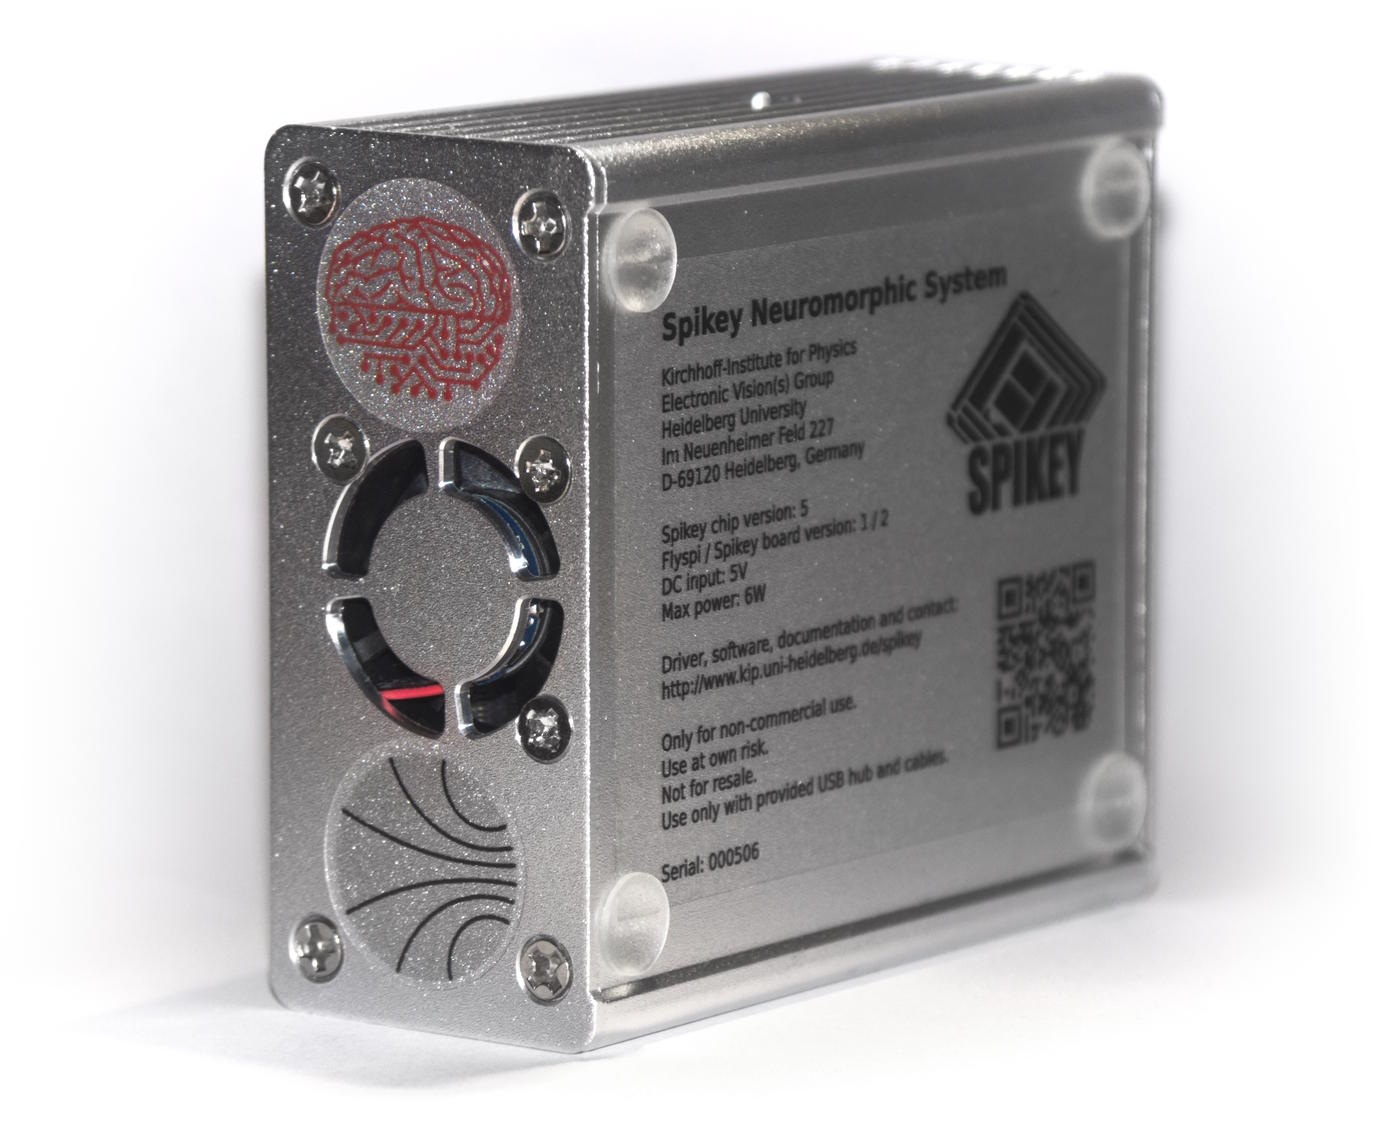
\includegraphics[width=0.475\textwidth]{media/chp1/spikey_photo.jpg}
		\label{fig:spikey_photo}
	}
	\subbottom[Spikey chip bonded to the circuit board]{
		\centering
		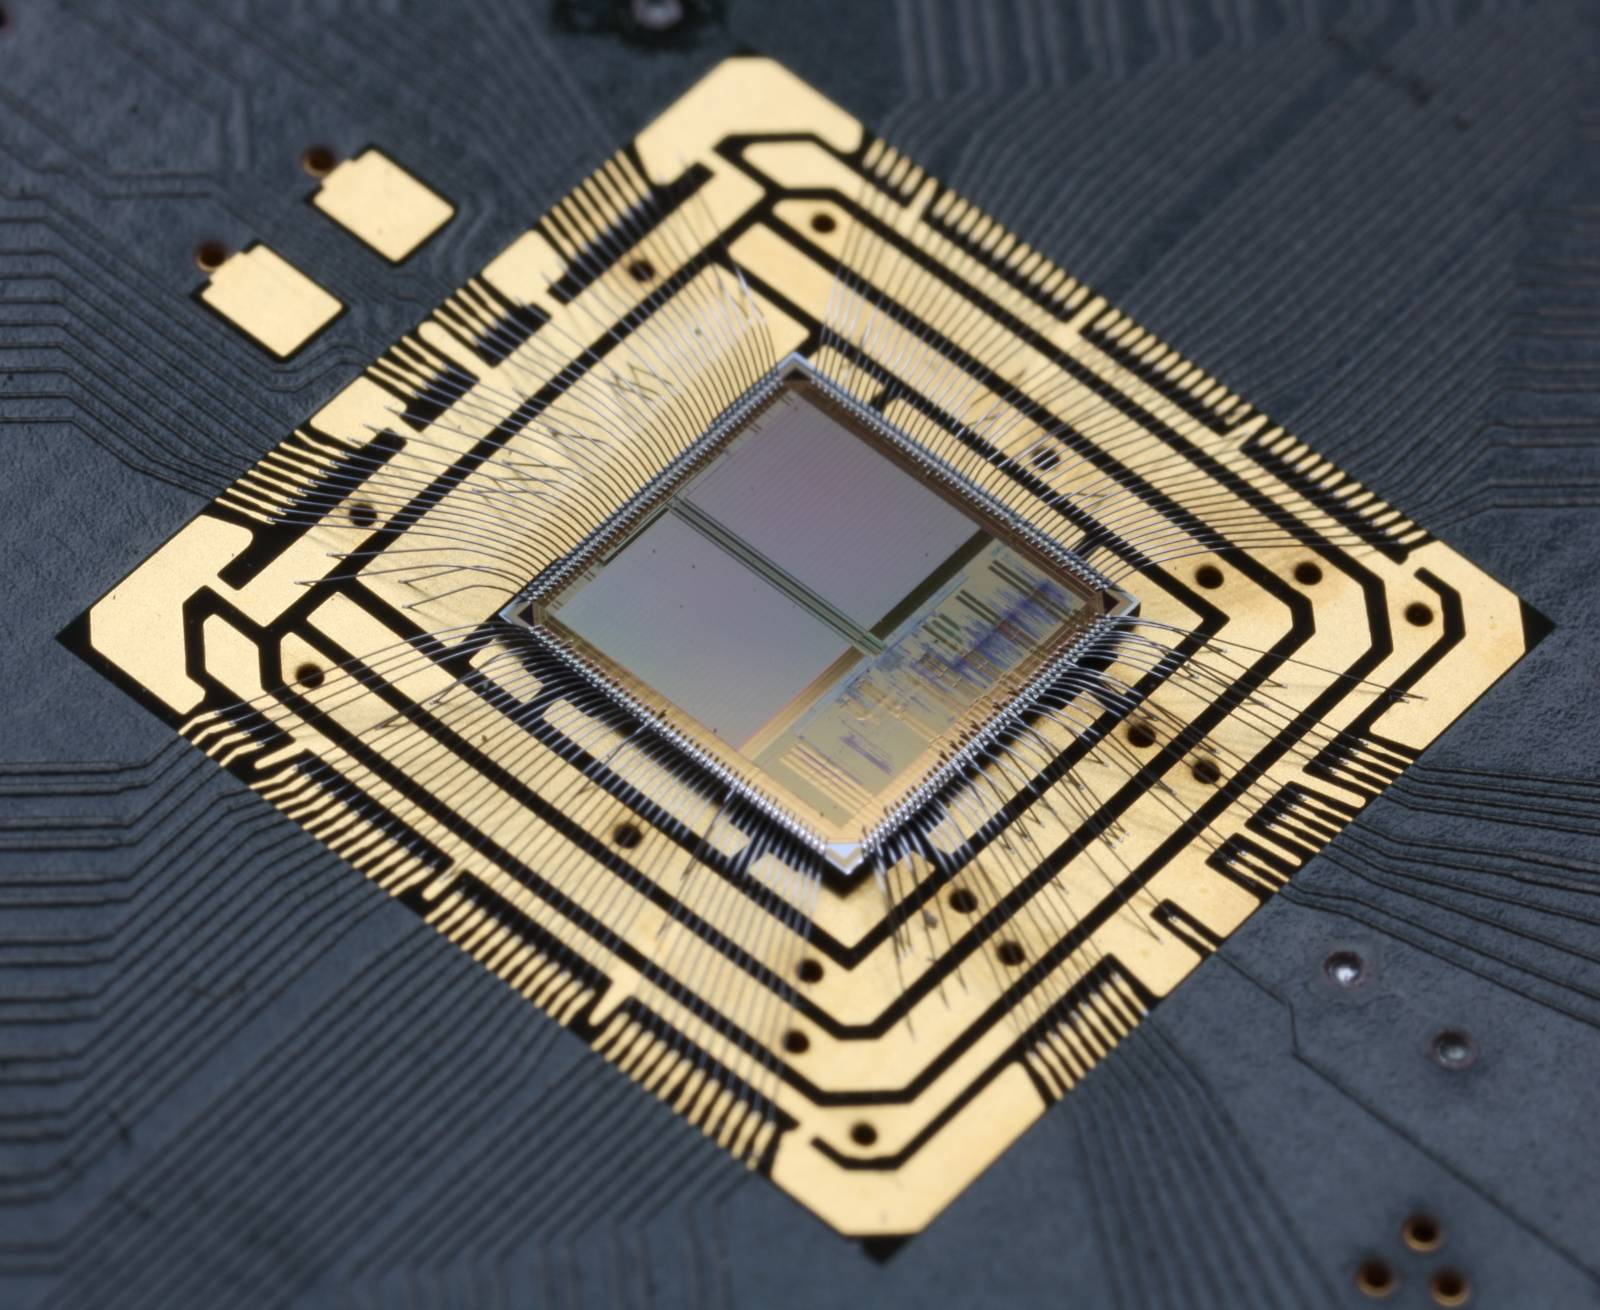
\includegraphics[width=0.475\textwidth]{media/chp1/spikey_chip_cropped.jpg}
		\label{fig:spikey_chip}
	}
	\caption[Photos of the Spikey neuromorphic hardware system]{Photos of the \emph{Spikey} neuromorphic hardware system developed by the Electronic Visions group at Heidelberg University. Size of the assembled device in (a) is about $8 \times 7 \times 3 \, \si{\centi\meter}$; the picture of the actual chip in (b) is copied from \url{http://www.kip.uni-heidelberg.de/spikey}.}
	\label{fig:spikey}
\end{figure}
\marginnote{A more technical description of the neuromorphic systems can be found in \cref{sec:neuromorphic_hardware}.}
The two neuromorphic hardware systems developed in the \acrshort{HBP} possess fundamentally different architectures. The \enquote{many-core system} \acrshort{NMMC} built at the University of Manchester is a fully digital computer, constructed around the \emph{SpiNNaker} chip \cite{furber2013overview}. In contrast, the \enquote{physical model} (\acrshort{NMPM}) built at Heidelberg University, is an analogue-digital mixed signal system composed of entire silicon wafers of \emph{HICANN} (\acrlong{HICANN}) chips \cite{schemmel2010wafer,bruderle2011comprehensive}. Both systems offer significantly faster simulation times for large spiking neural networks compared to software simulations on supercomputers, with \acrshort{NMMC} executing large networks at biological timescale and \acrshort{NMPM} with a speedup of $10\,000$ compared to biological timescale.

A third system -- which is used in addition to the already mentioned ones -- is the \emph{Spikey} neuromorphic system (\cref{fig:spikey}). The Spikey chip at its core is a predecessor of the HICANN in \acrshort{NMPM}. As such, it shares the same speedup factor of $10\,000$, but is limited to a single chip and features a less complex neuron model \cite{pfeil2013six}. Since Spikey has been in development for almost a decade now, both its hardware and software are in a relatively mature state.

\subsection{Willshaw associative memory as a spiking neural network}

\marginnote{Artificial neural networks in general and spiking neural networks in particular are discussed in \cref{sec:neural_network_models,sec:biophysical_neuron_model,sec:spiking_neuron_models}.}
Due to their time dynamic and asynchronous nature, spiking neural networks are difficult to design: every neuron possesses a multitude of parameters, and small changes in a single neuron parameter can dramatically influence the behaviour of the network as a whole. This is already true for the most simple class of network topologies, so called feed-forward networks, which do not allow recurrent connections (cycles in the network graph). On the other hand, it is reasonable to assume that biological neural networks have evolved with a robustness to neuronal variation. Indeed, the same neural circuits in two animals have been found to produce similar output on the network-level, although the intrinsic configuration of individual neurons varies significantly between the animals  \cite{prinz2004similar, marder2011multiple}.

\marginnote{The Willshaw associative memory model is described in detail in \cref{sec:willshaw_theory}.}
As the Willshaw associative memory model merely is a theoretical concept, that was not designed with the perils of dynamical systems in mind, it describes no mechanism that would allow for the compensation of neuronal imprecisions. On the contrary, each output signal is produced independently by a single artificial neuron. There is no possible way in which coarsely estimated neuron parameters could be absorbed by network-level effects. For the transition of the theoretical memory architecture to a spiking neural network we could proceed in two different ways. By designing robust sub-networks for each theoretical neuron from which the desired behaviour emerges, or by literally translating the theoretical model to a spiking neural network and tuning the neuron parameters to precise values.

We have decided to take the second approach. We aim at small and simple networks which only deviate slightly from the theoretical model, to ensure that the exhaustive theoretical results regarding the memory still apply. However, in order to find suitable neuron parameters, we need to provide an at least semi-automatic method which lets us choose \enquote{optimal} parameters for a given memory configuration.

\subsection{Associative memories as hardware benchmark}

The above decision on the spiking network architecture opens the door for another application. Since the network is scalable, possesses a highly regular and simple structure, and its theoretical behaviour under perfect conditions is well understood, it can serve as a hardware benchmark. Such a benchmark can be used to compare the performance of the individual platforms, and to quantify the influence of hard- and software changes.

Providing an assessable benchmarking network is important, as the \acrshort{HBP} hardware platforms (excluding Spikey) are currently in an early stage of development and running even simple networks reliably on all platforms is likely to be enough of a challenge. Ideally, sweeps along multiple parameter axes of the design space can be performed. This would allow to find regions for which the system shows abnormal behaviour. For example, varying the memory size might uncover scaling issues.

\subsection{Goals of this thesis}

The top-level goal of this thesis is to provide a working Willshaw associative memory (\acrshort{BiNAM}) implementation as spiking neural network which can be executed on the mentioned neuromorphic hardware systems. In order to fulfil this goal for varying memory configurations (\eg size, data properties), we need to find a way to explore the network design space. This requires that we have defined the design space itself and performance measures we can assign to every point in the space.

Unfortunately, and unsurprisingly, the design space is high-di\-men\-sion\-al, which prevents any exhaustive exploration. Therefore, we intend to develop and evaluate estimations of the network performance. These should allow an interactive exploration of a two-dimensional projection of the design space and help to restrict the parameter space to regions, in which time-consuming network simulations (potentially accelerated by the neuromorphic hardware) are sensible. Additionally, it should be possible to use the performance estimations for automatic parameter optimisation.

These goals also come with a significant engineering task, as the software tools for interactive design space exploration, parameter optimisation and execution on the hardware platforms have to be implemented. Finally, we have to investigate whether the built tools can be reliably used for benchmarking.

\section{Structure}
\label{sec:structure}

Whereas \cref{sec:motivation_goals} approached the topics in this thesis from a bird's-eye perspective and in no particular order, this section linearly trudges along the chapters and traces the golden thread which guides through the pages to come.

In \cref{chp:related_work}, we start by summarising the related work that sits at the foundation of this thesis: we touch the relevant neurobiological basics, introduce notable neuron and neural network models, and present the neuromorphic hardware platforms and software simulators. Finally, the Willshaw associative memory model (\acrshort{BiNAM}) is described and compared to other models.

In order to transition the theoretical \acrshort{BiNAM} model to a spiking neural network, \cref{chp:spinam} defines a parametrised set of spiking \acrshort{BiNAM} implementations. Combined with the neuron model parameters, these implementation parameters span the associative memory design space we seek to explore. Various associative memory evaluation measures are then proposed, which allow the assignment of a set of scores to any given point in the design space. As a side-effect, these measures allow comparison -- and eventually benchmarking -- of different hardware and software platforms. The chapter concludes with thoughts on \acrshort{BiNAM} test data generation. In its entirety, the material in \cref{chp:related_work,chp:spinam} allows the construction of a complete \acrshort{BiNAM} design space exploration pipeline.

Armed solely with the methods described beforehand, however, any even rudimentarily exhaustive design space exploration would be infeasible, regardless of neuromorphic hardware acceleration. Thus, \cref{chp:neuron_evaluation} takes a step back and describes \acrshort{BiNAM} performance estimates of varying complexity, based on single neuron simulation. To achieve the fastest possible execution speed, we compare the performance of various numerical differential equation integration methods. Finally, a method for fractional neuron output spike count estimation is presented, which in conjunction with a naive Downhill-Simplex algorithm effectively allows automated neuron parameter optimisation with respect to a given set of network parameters. The presented work can be used to limit the parameter space to interesting regions, which can then be explored by means of expensive full network simulations.

Such simulations are conducted in \cref{chp:experiments}, which describes experiments testing the evaluation measures defined in \cref{chp:spinam} on the neuromorphic hardware platforms. The hardware results are then compared to software simulations and the coarse estimates from the fourth chapter.

Finally, \cref{chp:conclusion} summarises the insights obtained and lists possible future work that was out of scope for this thesis.

\section{Notational conventions}
\label{sec:notation}

\marginnote{Margin notes contain additional remarks or small sketches which aim at providing a better understanding of the material -- however, they can be safely skipped; all relevant information is presented in the main text.}
This section informally lists some important notational conventions employed throughout the thesis.

\paragraph{Symbols}
Great care has been taken to consistently impose a single meaning on most mathematical symbols. Exceptions to this rule are \enquote{local variables}, including -- but not limited to -- the symbols $i, j, k, \ell$ which are used as generic indices, for example as summation indices, loop counters or to point at a generic element of a set, tuple, vector or matrix. The meaning of symbols used in more than one occasion can be looked up in the symbol overview in the appendix.

\paragraph{Vector and matrix indices}
Vectors are marked as such with a vector arrow and are generally assumed to be column vectors. If individual matrix or vector elements are accessed, this is denoted as $(\vec x)_i$ (the $i$-th component of $\vec x$) or $(M)_{ij}$ (the element in the $i$-th row and $j$-th column of the matrix $M$) respectively. An exception to this rule are algorithms in pseudo-code where individual vector and matrix elements are accessed in the \enquote{square brackets}-notation, for example $\vec x[i]$ and $M[i, j]$. Regardless of the notation, vector and matrix indices follow the mathematical convention and always start with one.

\paragraph{Sets and tuples}
Sets are usually typeset in fraktur (\eg $\mathfrak{b}$, $\mathfrak{B}$). Double-struck letters (\eg $\B, \N, \R$) denote ranges of numbers. The operator \enquote{$\Arrowvert$} denotes the concatenation of two tuples: let $a = (a_1, \ldots, a_i)$ and $b = (b_1, \ldots, b_j)$ denote two sequences of length $|a| = i$ and $|b| = j$. The operation $a \Arrowvert b$ is then defined as:
\begin{align}
	a \Arrowvert b = (a_1, \ldots, a_i, b_1, \ldots, b_j)
\end{align}

\paragraph{Discontinuities in differential equations}
Spiking neural network models are generally formulated as differential equations. However, they contain discontinuities which often are expressed in the literature with the help of the Dirac delta $\delta(t)$:
\begin{align}
 	\int_{-\infty}^{\infty} f(t) \cdot \delta(t) \; \mathrm{d}t = f(0) \,.
\end{align}
Use of the Dirac delta may facilitate mathematical analysis, but in the opinion of the author tends to obscure the actual concept that is being described. We therefore use a less mathematical notation which involves the \enquote{$\gets$} (read \enquote{gets}) operator. For example, a differential equation with a discontinuity at time $t_0$ is described as
\begin{align}
	\dot u(t) &= g \cdot (u(t) - u_0) \,,\\
	u(t) &\gets u(t) + \Delta u \quad \text{if } t = t_0\,,
\end{align}
and supposed to be equivalent to the more \enquote{correct} mathematical notation
\begin{align}
	\dot u(t) = g \cdot (u_0 - u(t)) + \delta(t - t_0) \cdot \Delta u\,.
\end{align}

\chapter{Background and Related Work}
\label{chp:related_work}

\epigraph{The study is to proceed on the basis of the conjecture that every aspect of learning or any other feature of intelligence can in principle be so precisely described that a machine can be made to simulate it. \textnormal{[...]} We think that a significant advance can be made in one or more of these problems if a carefully selected group of scientists work on it together for a summer.}{McCarthy et al., 1955, Proposal for the Dartmouth conference}

The primary goal of this thesis is to implement an associative memory model as a spiking neural network on top of neuromorphic hardware. In this chapter we aim at providing a terse summary of the mentioned fields: \cref{sec:neural_network_models,sec:biophysical_neuron_model,sec:spiking_neuron_models} address artificial neural network models in general, the neurobiological concepts inspiring spiking neural networks, relevant spiking neuron models, and their parameters. \cref{sec:neuromorphic_hardware} focuses on the neuromorphic hardware systems in the \HBP. In \cref{sec:willshaw_theory} we discuss the notion of associative memories and expand on the Willshaw associative memory model relied upon in this thesis.

%
% HISTORY OF ARTIFICIAL NEURAL NETWORK MODELS
%

\section{History of artificial neural network models}
\label{sec:neural_network_models}

In 1780 Luigi Galvani discovered that the injection of electric potentials into animal muscle tissue causes contractions. He was the first to notice that electricity could play a role in the animation -- or liveness -- of animals and laid the groundwork for research concerning electrophysiology \cite{piccolino1997luigi}.

Sixty-eight years later, in 1848, Emil du Bois-Reymond discovered discrete electrical pulses generated by nerve cells \cite{pearce2001emil}. It took another seventeen years until Julius Bernstein (supported by du Bois-Reymond) could successfully record one of these \emph{action potentials} or \emph{spikes} on paper. Today we know that action potentials are the primary way of encoding information in the nervous system \cite{schuetze1983discovery}.

\begin{figure}
	\small
	\centering
	\subbottom[Pyramid cells]{
		\centering
		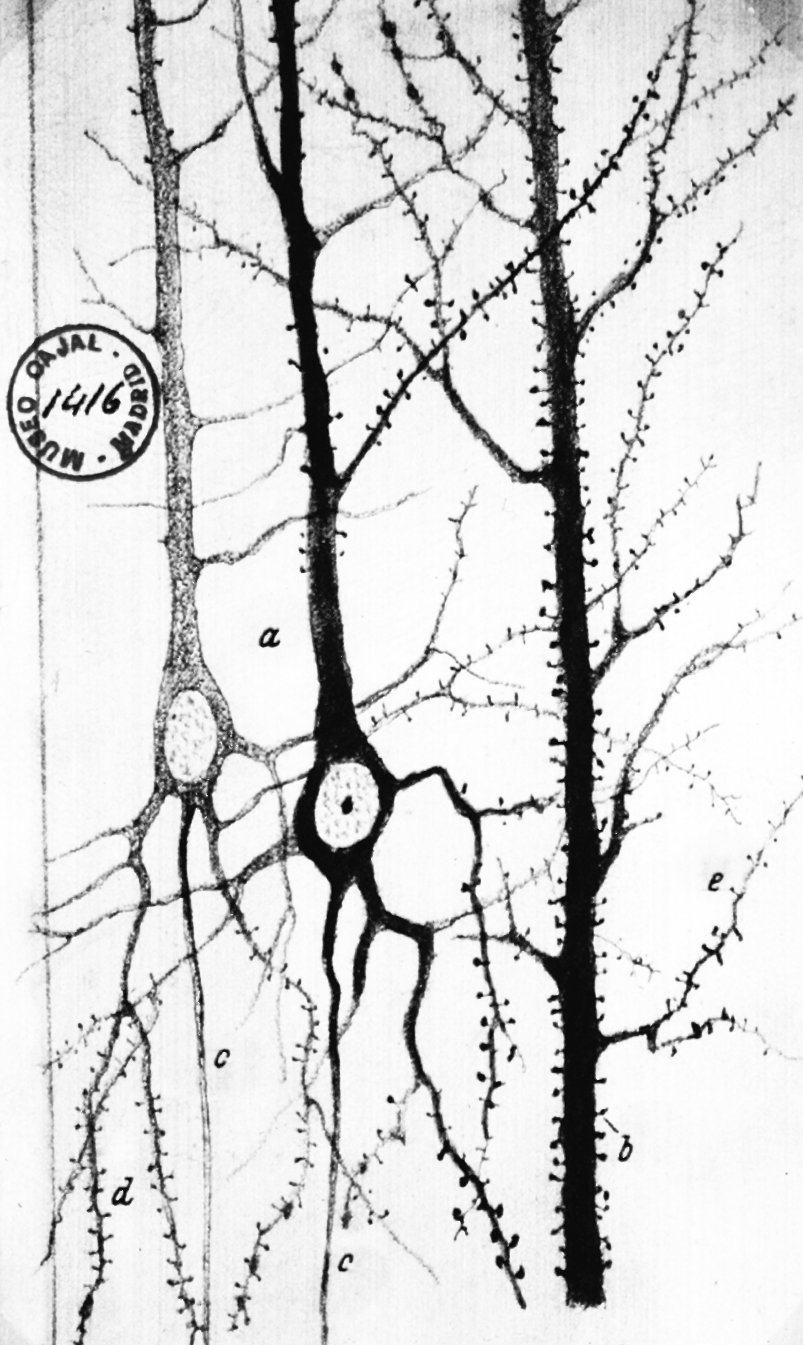
\includegraphics[height=7cm]{media/chp2/cajal_pyramid_cell.png}
		\label{fig:cajal_pyramid_cell}
	}
	\hspace*{0.75cm}
	\subbottom[Neurons in spinal marrow]{
		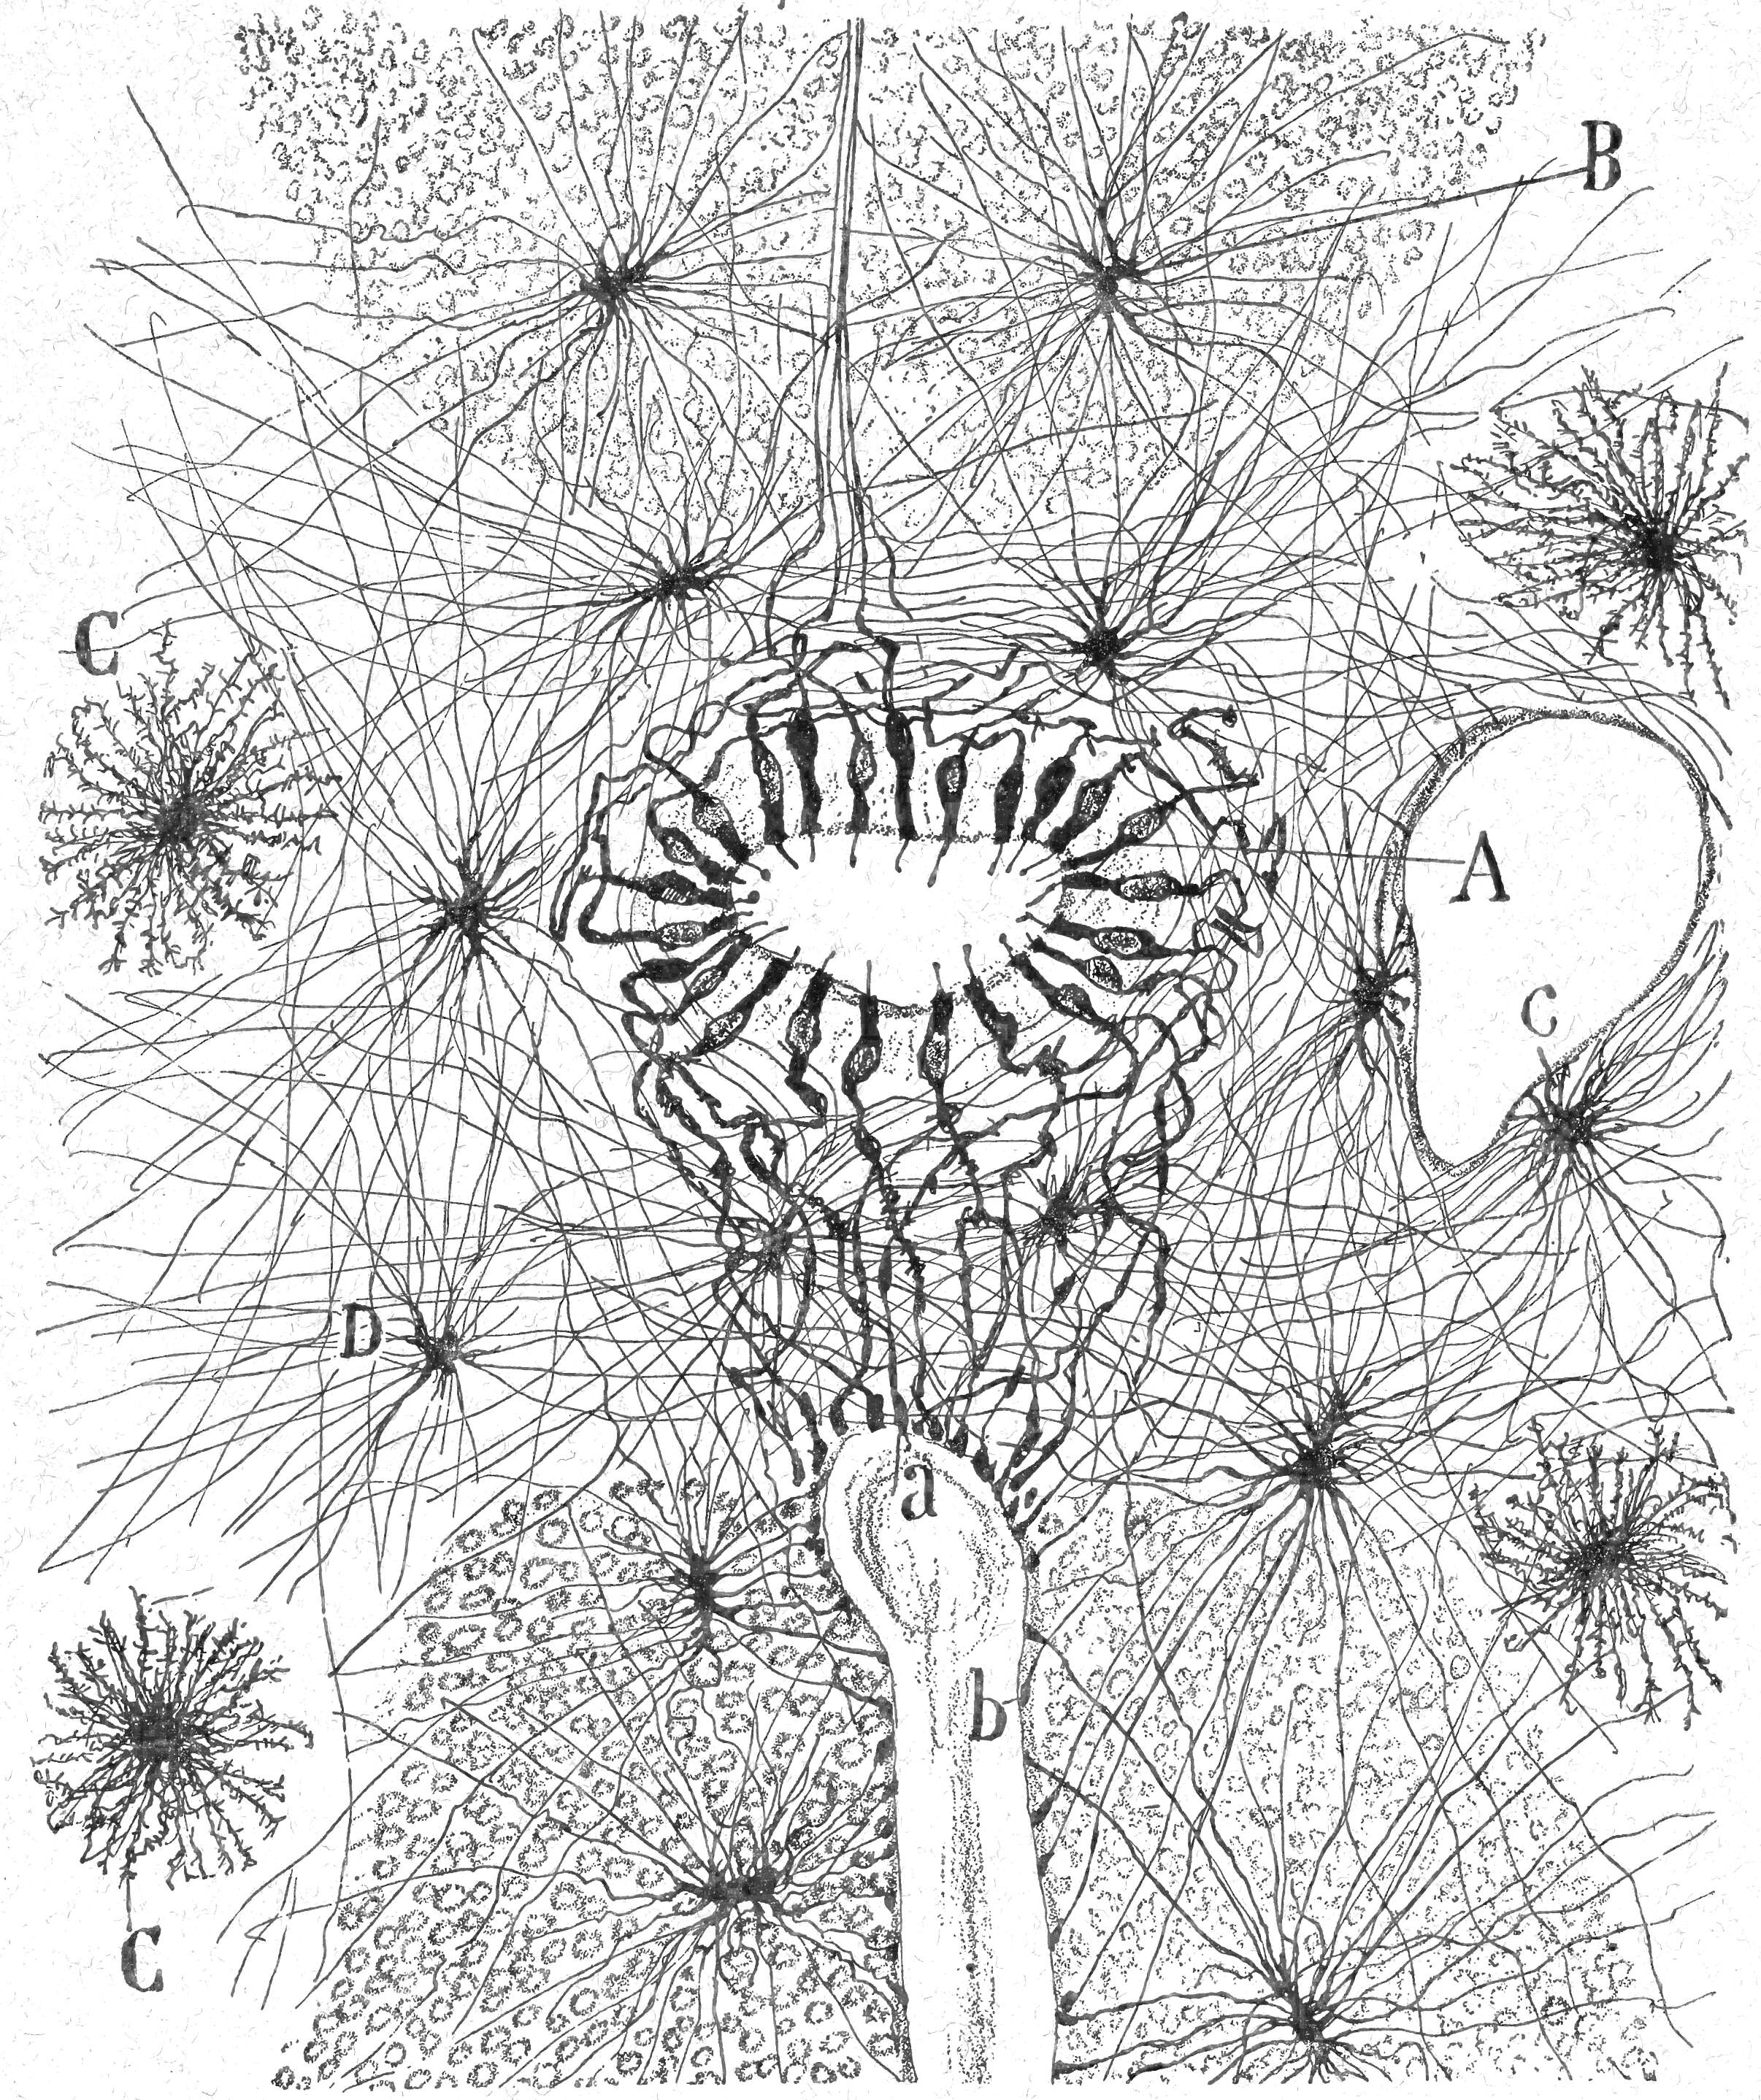
\includegraphics[height=7cm]{media/chp2/cajal_neuroglia.jpg}
		\label{fig:neurons_shape}
	}
	\caption[Drawings by Santiago Ramón y Cajal]{Neural tissue prepared using Golgis method and drawn by Santiago Ramón y Cajal around 1900. (a) shows pyramidal neurons in brain tissue, (b) neurons of varying shape in the white spinal marrow substance \cite{ramon1904textura}.}
	\label{fig:cajal}
\end{figure}
At the end of the nineteenth century, technological advances in microscopy and a new staining method invented by Camillo Golgi allowed scientists to examine individual neurons in brain and spinal tissue samples (\cref{fig:cajal}). In 1887 Santiago Ramón y Cajal was the first to propose neurons as distinct base units of information processing in biological systems. For their work Golgi and Cajal received the 1906 Nobel prize. Their discoveries gave rise to the \emph{neuron doctrine}, the idea that spinal cord and brain are made of basic building blocks -- neurons -- and their support structures \cite{glickstein2006golgi}.

As the understanding of the neurobiological mechanisms advanced, another question began to dawn in the scientific world: if animal -- and human -- behaviour was solely determined by the electrophysiological properties of neural networks, could it not be possible to build machines that simulate processes in the brain up to cognition and intelligence? In the 1940s researchers began to construct mathematical models which mimic structural properties of biological neural networks. The development of artificial neural networks since then can be broken down into three distinct generations \cite{maass1997networks}.

\subsection{First generation: binary McCulloch-Pitts cells}
\label{sec:mcculloch_pitts_neuron}

\marginfig{Sketch of a McCulloch-Pitts artificial neuron}{
	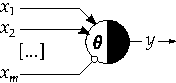
\includegraphics{media/chp2/mcculloch_pitts_neuron.pdf}
	\vspace{0.25cm}
}{Sketch of a McCulloch-Pitts neuron: excitatory (arrow) and inhibitory (circle) inputs are accumulated. If a threshold $\theta$ is passed, the output $y$ is set to one, zero otherwise.}{\label{fig:mcculloch_pitts_neuron}}
In 1943 Warren McCulloch and Walter Pitts proposed the first artificial neural network model. In order to cope with the high diversity and complexity of biological neurons, their model is based on several simplifying assumptions: the nervous system is built of a network of neurons, each consisting of a cell body (\emph{soma}) and an axon. They gather input from connected neurons through excitatory or inhibitory synapses located at dendritic extensions of the soma (\emph{dendrites}). If the excitation of a neuron passes a threshold, the neuron responds with a binary \enquote{all-or-none} spike, that travels along the axon to other neurons, where it is received as input (\cref{sec:biophysical_neuron_model,fig:neuron_sketch}).
\begin{figure}
	\centering
	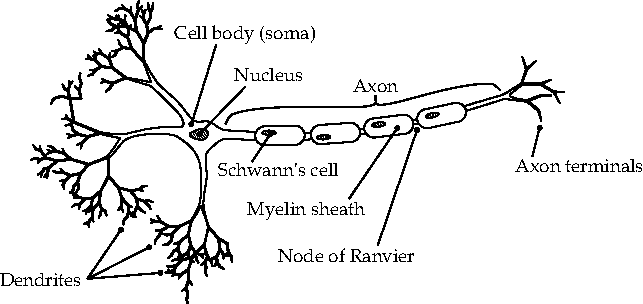
\includegraphics[width=\textwidth]{media/chp2/neuron_sketch.pdf}
	\caption[Sketch of a schematised model neuron]{Sketch of a schematised biological model neuron. Input spikes arrive at synapses located at the dendrites and are processed in the cell body. Resulting output spikes travel along the axon to the axon terminals, which connect to other neurons or a neuromuscular junction. Inspired by \cite{kandel2012principles}.}
	\label{fig:neuron_sketch}
\end{figure}
Furthermore, McCulloch and Pitts argue that transmission of signals along the axon is almost instantaneous and considerable delay occurs only at the synapses. This allows to disregard spike times and instead synchronously propagate binary values between neurons in discrete time steps \cite{mcculloch1943logical}.

\marginfig{McCulloch-Pitts artificial neuron as Boolean operators}{
	OR ($y = x_1 \vee x_2$):\\
	\vspace{0.25cm}
	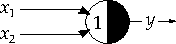
\includegraphics{media/chp2/mcculloch_pitts_neuron_or.pdf}
	\vspace{0.5cm}\\
	AND ($y = x_1 \wedge x_2$):\\
	\vspace{0.25cm}
	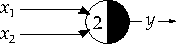
\includegraphics{media/chp2/mcculloch_pitts_neuron_and.pdf}
	\vspace{0.5cm}\\
	NOT ($y = \neg x$):\\
	\vspace{0.25cm}
	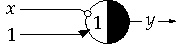
\includegraphics{media/chp2/mcculloch_pitts_neuron_not.pdf}
	\vspace{0.25cm}
}{McCulloch-Pitts artificial neuron as Boolean operators.}{\label{fig:mcculloch_pitts_neuron_logic}}
Mathematically, a single McCulloch-Pitts cell with binary input vector $\vec x = \transpose{(x_1, \ldots, x_m)} \in \B^m$, output $y \in \B$, and $\B = \{0, 1\}$ can be described as follows (\cref{fig:mcculloch_pitts_neuron})
\begin{align}
	y &= \Heaviside(\transpose{\vec w} \cdot \vec x - \theta) & \text{where} \quad 
		\Heaviside(x) &=  \begin{cases}
			1 & \text{if } x \geq 0 \\
			0 & \text{otherwise}
	    \end{cases} \,.
	\label{eqn:mcculloch_pitts_cell}
\end{align}
The weights $\vec w = \transpose{(w_1, \ldots, w_m)} \in \{-1, 1\}^m$ model excitatory ($w_i = 1$) or inhibitory ($w_i = -1$) synaptic connections to the input $x_i$, the threshold $\theta \in \mathbb{Z}$ describes the minimum excitation that causes a \enquote{one} as output. The function $\Heaviside(x)$ is also called \enquote{Heaviside step function}.

As shown in \cref{fig:mcculloch_pitts_neuron_logic}, the cells can be used to construct the basic operators of Boolean algebra. It follows that any computable function can be described by a large network of McCulloch-Pitts cells -- they are Turing complete \cite{copeland1996alan}.

\subsection{Second generation: firing-rate coded neural networks}

In 1958 Frank Rosenblatt extended the binary McCulloch-Pitts cell to the so called \enquote{perceptron}. Weights $w_i$ and neural input $x_i$ in \cref{eqn:mcculloch_pitts_cell} are now real-valued instead of binary. Biologically, this change can be motivated by the observation that some neurons operate in a mode known as \enquote{tonic spiking} in which they output discrete spikes at a certain rate that monotonously depends on the excitation of the neuron (Figures \ref{fig:neuron_behaviours}(a) and \ref{fig:neuron_behaviours}(g)). The real valued input $\vec x \in \R^m$ can be interpreted as the average firing-rate of the pre-synaptic neuron, the weights $\vec w \in \R^m$ describe the influence of a synapse on the excitation of the neuron \cite{haykin2011neural}.

Rosenblatt's most important contribution, though, is a learning rule which allows to train the weights $\vec w$ in such a way, that the perceptron outputs a desired answer $y_k$ for a certain input $\vec x_k$, allowing to solve linear classification and regression tasks \cite{minsky1987perceptrons}.

\marginfig{Sketch of a classical artificial neuron}{
    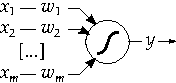
\includegraphics{media/chp2/classical_neuron.pdf}
    \vspace{0.25cm}
}{Sketch of a firing-rate coded artificial neuron. Each neuron in the network computes the weighted sum of inputs $x_1, \ldots, x_m$, applies a non-linearity $f$ and outputs an activation value $y$ that might be fed into other neurons or act as part of the network output.}{\label{fig:classical_neuron}}
In the context of the feed-forward \MLP, the neuron model is generalised to the \enquote{firing-rate artificial neuron}, replacing the Heaviside function $\Heaviside$ with an arbitrary non-linear, sigmoid function $f$ and fusing the threshold $\theta$ as an additional dimension (\enquote{bias}) into the input $\vec x$ and the weights $\vec w$ (\cref{fig:classical_neuron})
\begin{align}
	y = f(\transpose{\vec w} \cdot \vec x) \,.
\end{align}
The weights $\vec w$ of the individual neurons in a \MLP can be easily trained using the back-propagation algorithm (a generalisation of Rosenblatt's perceptron learning rule). Today, with the broad availability of massively parallel computing hardware, large {\MLP}s with many hidden layers are employed with success in the field of \enquote{deep learning} \cite{hinton2006fast}.

\subsection{Third generation: spiking neural networks}

McCulloch and Pitts assumed that coarse, discrete timesteps are sufficient for the propagation of neural output -- a paradigm that is adopted by second generation networks. Experiments suggest however, that exact spike timing and spike time correlation within neuron populations are used to encode information in the nervous system \cite{shadlen1994noise}. At the end of the 1980s, these discoveries gave rise to the third generation of neural networks, in which neurons are simulated as dynamical systems with asynchronously generated binary spikes \cite{maass1997networks}.

Besides being closer to biology, spiking neural networks have several practical advantages over their predecessors: whereas firing-rate models require the transfer of the neuron state of every neuron in every time step, the asynchronicity of spiking networks only requires communication whenever a neuron generates a spike. Due to the loose coupling of individual neurons, spiking networks lend themselves to be simulated energy efficiently on massively parallel, asynchronous hardware. Furthermore, given their time-dynamic nature, spiking neural networks intrinsically process time series of data.

On the other hand, simulation of neuron time dynamics is computationally intensive, training of spiking networks is more complicated compared to their firing-rate counterpart and -- at least for simple models -- biological plausibility is still limited: usually neither spatiality, nor the influence of neuromodulators are simulated. Nevertheless, spiking neural networks may provide a useful simulation platform for entire brain circuits \cite{johansson2007towards} and may in the future allow to simulate deep networks on specialised, energy efficient hardware \cite{hasler2013finding,schmidhuber2015deep}.

We continue with a description of the spiking neural network models this thesis is based on in \cref{sec:spiking_neuron_models}, but before, in \cref{sec:biophysical_neuron_model}, we quickly explore their biological basis.

%
% BIOPHYSICAL NEURON MODEL
%

\section{Biophysical neuron model}
\label{sec:biophysical_neuron_model}

Biological observations of neuronal behaviour have (amongst others) been captured in the biophysically meaningful \HH neuron model, introduced in 1952  \cite{hodgkin1952quantitative}. It builds the basis of most simplified spiking neural network models in neuroinformatics. In the remainder of this section we discuss the relevant parts of this model.

\subsection{Passive electrophysiological properties of the neuron membrane}
\label{sec:electrophysiological_properties}

\marginnote{Ions in the intra-/extra\-cel\-lu\-lar fluid which usually play a role in neurobiological processes are: sodium ions \(\mathrm{Na}^+\), chloride \(\mathrm{Cl}^-\), potassium ions \(\mathrm{K}^+\), calcium ions \(\mathrm{Ca}^{2+}\), as well as negatively charged amino acids \(\mathrm{A}^-\).}
The electrical properties of a single neuron are caused by a different ion compositions in intra- and extracellular fluid, and selectively permeable ion channels in the cell membrane. When measuring the electrical potential between the intra- and extracellular space -- the \emph{membrane potential} {\um} -- of an inactive neuron, one finds the intracellular space being more negatively charged than the extracellular space \cite{kandel2012principles}. This particular voltage is called the \emph{resting} or \emph{leak} potential \El.

\begin{figure}
	\centering
	\subbottom[Membrane without \(\mathrm{K}^+\)-channel]{%
		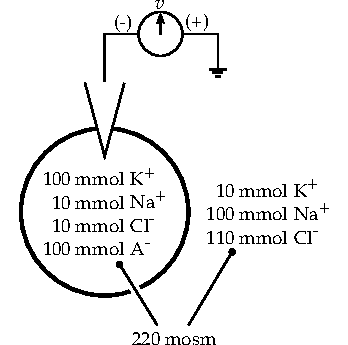
\includegraphics{media/chp2/neuron_channel_a.pdf}%
		\label{fig:neuron_channel_a}
	}%
	\subbottom[Added \(\mathrm{K}^+\)-channel]{%
		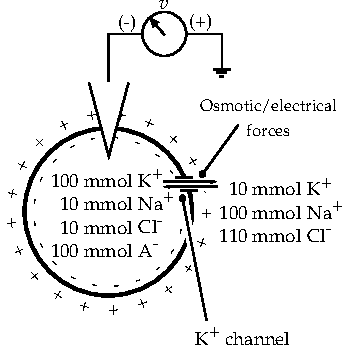
\includegraphics{media/chp2/neuron_channel_b.pdf}%
		\label{fig:neuron_channel_b}
	}
	\caption[Membrane potential change caused by selectively permeable ion channel]{Ion compositions in intra- and extracellular space and with closed (a) and opened (b) selectively permeable ion channel. See \cref{sec:electrophysiological_properties} for a description. Adapted from \cite{kandel2012principles}.}
\end{figure}
An examination yields differences in the intra- and extracellular fluid ion-composition, with the intracellular composition being maintained by ion pumps in the cell membrane. However, seemingly contradictory to the previous result, both fluids are electrically neutral and have the same osmotic concentration. Only if the membrane was a perfect insulator -- as assumed in \cref{fig:neuron_channel_a} --, there would be no measurable potential.

\marginnote{The number of ions involved in the generation of the equilibrium potential is negligibly small compared to the total number of ions in the cell.}
Experiments show, that the membrane contains selectively permeable ion channels. In its resting state, the membrane is mostly permeable for potassium ions $\mathrm{K}^+$. Due to the difference between intra- and extracellular ion concentration, an osmotic force causes \(\mathrm{K}^+\) to flow out of the cell. The total ionic current is proportional to the number channels in the membrane, or its \emph{permeability} for \(\mathrm{K}^+\). Missing \(\mathrm{K}^+\) cause the intracellular fluid to become slightly negatively charged, creating a countering electric force on the positively charged ions. As sketched in \cref{fig:neuron_channel_b}, the system converges towards an equilibrium state with potential $E_{\mathrm{Eq}}$ in which osmotic and electric force are equal.

Consider the equilibrium potential $E_{\ion}$ for a membrane that is permeable for an ion species \ion only. We refer to $E_{\ion}$ as the \emph{reversal potential} for \ion: its ionic current reverses at this potential. For intra- and extracellular ion concentrations $[\ion]_{\mathrm{in}}$ and $[\ion]_{\mathrm{out}}$, $E_{\ion}$ is given according to the Nernst equation as
\begin{align}
	E_{\ion} &= \frac{R \cdot T}{z \cdot F} \cdot \ln\left( \frac{[\ion]_{\mathrm{out}}}{[\ion]_{\mathrm{in}}} \right){,}
	\label{eqn:nernst}
\end{align}
where $R$ is the ideal gas constant, $T$ the temperature in Kelvin, $F$ Faraday's constant, and $z$ the ion charge in elementary charges \cite{kandel2012principles}.
Given the (relative) permeabilities or \emph{conductances} $g_{\ion}$ of the cell membrane for each ion species \ion, the equilibrium potential $E_{\mathrm{eq}}$ can be calculated according to the Goldman–Hodgkin–Katz equation as
\begin{align}
	E_{\mathrm{eq}} = \frac{\sum\nolimits_{\ion} g_{\ion} \cdot E_{\ion}}{\sum\nolimits_{\ion} g_{\ion}} = \frac{\sum\nolimits_{\ion} g_{\ion} \cdot E_{\ion}}{g_{\mathrm{tot}}} \,.
	\label{eqn:membrane_base}
\end{align}
\marginnote{Correspondence between Fig.~\ref{fig:membrane_base} and Eq.~(\ref{eqn:membrane_base}) can be easily shown using Kirchhoff's laws.}
The behaviour modelled by \cref{eqn:membrane_base} corresponds to an electric circuit, consisting of parallel voltage sources with voltage $E_{\ion}$ and a series resistor with conductance $g_{\ion}$ for each ion channel (\cref{fig:membrane_base}).

\begin{figure}
	\small
	\centering
	\begin{circuitikz}
		\draw[->] (-1.5, 0.5) -- node[left] {\Eeq} (-1.5, 3.5);
		\draw(0, 4) to[R, l=$g_{\mathrm{K}^+}$] (0, 2);
		\draw(0, 2) to[battery1, l=$E_{\mathrm{K}^+}$] (0, 0);
		\draw(2, 4) to[R, l=$g_{\mathrm{Na}^+}$] (2, 2);
		\draw(2, 0) to[battery1, l=$E_{\mathrm{Na}^+}$, mirror] (2, 2);
		\draw(4, 4) to[R, l=$g_{\mathrm{Cl}^-}$] (4, 2);
		\draw(4, 2) to[battery1, l=$E_{\mathrm{Cl}^-}$] (4, 0);
		\draw(-1.5, 0) to[short, o-*]
		     (0, 0) to[short,-*]
		     (2, 0) to[short,-*] (4, 0);
		\draw(-1.5, 4) to[short, o-*]
		     (0, 4) to[short,-*]
		     (2, 4) to[short,-*] (4, 4);
		\draw[dashed] (4, 0) -- (6, 0) -- (6, 1.85);
		\draw[dashed] (6, 2.15) -- (6, 4) -- (4, 4);
		\draw (6, 1.85) to[C, l=$\Cm$] (6, 2.15);
		\draw[->,dashed] (7, 0.5) -- node[right] {$\um(t)$} (7, 3.5);
	\end{circuitikz}
	\caption[Model equivalent circuit diagram of the neuron membrane for three ion channels]{Model equivalent circuit diagram of the neuron membrane for three ion channels. The potential that can be measured across the terminals on the left (without the capacitor) corresponds to the equilibrium potential as described in equation \cref{eqn:membrane_base}. Introducing a capacitor (dashed) with capacitance $\Cm$ transforms the circuit into the time-dynamic neuron base model in \cref{eqn:membrane_base_time}.}
	\label{fig:membrane_base}
\end{figure}
Due to inertia in the system, the membrane potential adapts slowly to any change, for example changes in the ion channel permeabilities. As depicted in \cref{fig:membrane_base}, this time-dynamic can be modelled by adding a capacitor with capacitance {\Cm} -- the \emph{membrane capacitance} -- in parallel to the equivalent circuit.

\begin{figure}
	\centering
	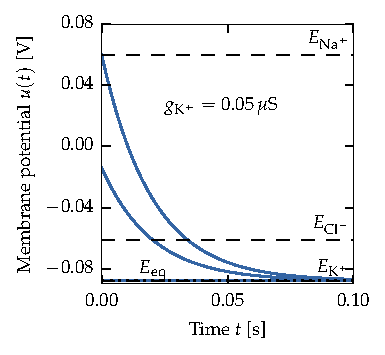
\includegraphics[trim=0.1cm 0.75cm 0.25cm 0.1cm,clip]{media/chp2/base_membrane_eq1.pdf}
	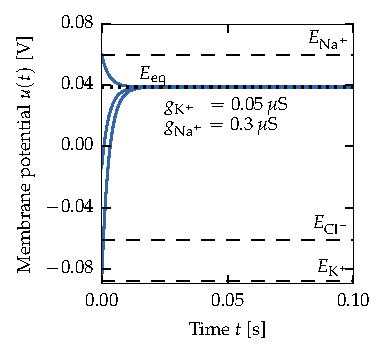
\includegraphics[trim=0.75cm 0.75cm 0.25cm 0.1cm,clip]{media/chp2/base_membrane_eq2.pdf}
	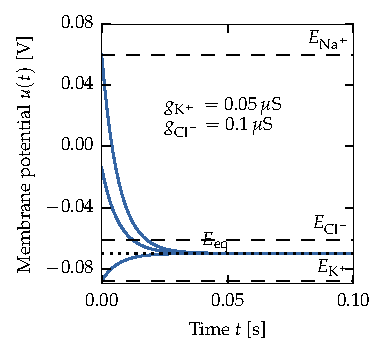
\includegraphics[trim=0.1cm 0.1cm 0.25cm 0.1cm,clip]{media/chp2/base_membrane_eq3.pdf}
	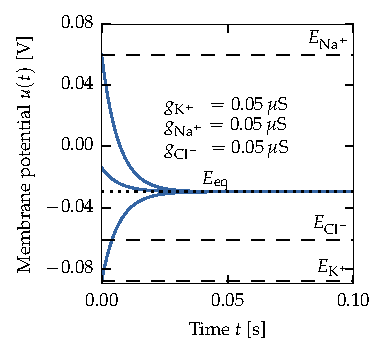
\includegraphics[trim=0.75cm 0.1cm 0.25cm 0.1cm,clip]{media/chp2/base_membrane_eq4.pdf}
	\caption[Membrane potential over time for varying membrane conductances]{Membrane potential over time for varying membrane conductances, according to \cref{eqn:membrane_base_time}. The reversal potentials are set to $E_{\mathrm{K}^+} = \SI{-88}{\milli\volt}$, $E_{\mathrm{Na}^+} = \SI{61}{\milli\volt}$ and $E_{\mathrm{Cl}^-} = -\SI{60}{\milli\volt}$, the membrane capacitance \Cm to $\SI{1}{\nano\farad}$.}
	\label{fig:membrane_base_time}
\end{figure}
\marginnote{By convention, positive currents $i(t)$ drive the membrane potential towards more negative values, negative currents towards more positive values.}
The time differential of the voltage across the capacitor \(\dum(t)\) is proportional to the current $i(t)$, which in turn is proportional to the difference \(\um(t) - \Eeq\). Hence, the circuit can be described as a linear differential equation
\begin{align}
	- \Cm \cdot \dot u(t) = i(t)
		&= g_{\mathrm{tot}} \cdot (u(t) - E_{\mathrm{eq}})
		 = \sum\nolimits_{\ion} g_{\ion} \cdot (u(t) - E_{\ion}) \,.
	\label{eqn:membrane_base_time}
\end{align}
\cref{fig:membrane_base_time} shows the system for varying $u_0$ and different membrane conductances. In all four plots the membrane is always slightly permeable for potassium ions \(\mathrm{K}^+\). If the membrane is not permeable for any other ion, this causes \(u(t)\) to slowly converge towards \(E_{\mathrm{K}^+}\). The velocity of the convergence is proportional to \(g_{\mathrm{tot}}\). Permeability for chloride or sodium ions pulls \(u(t)\) towards their reversal potential.

\subsection{Action potentials}

\begin{figure}
	\small
	\centering
	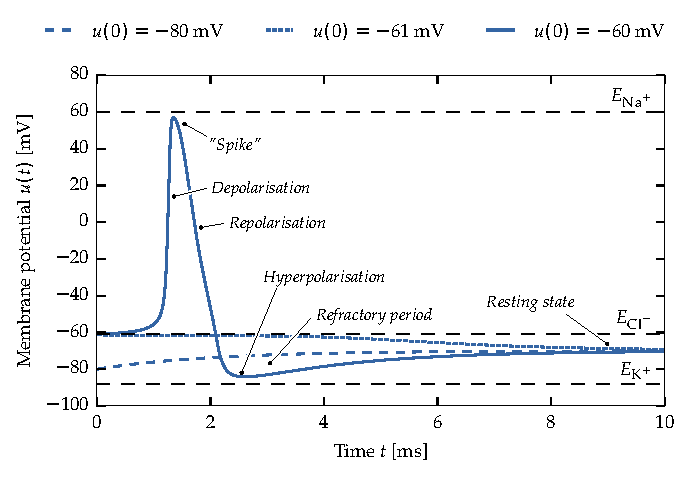
\includegraphics{media/chp2/hh_ap2_annotated.pdf}
	\caption[Annotated sketch of an action potential]{Annotated sketch of an action potential as produced by the \acrfull{HH} model. The membrane potential of three neurons is clamped to certain membrane potentials $\um(t)$ at $t = 0$. If a certain threshold potential is reached, the neuron generates an action potential; below this potential behaviour similar to a passive membrane can be observed.}
	\label{fig:action_potential_sketch}
\end{figure}

A passive cell membrane is not sufficient to explain action potentials and thus lacks an integral part of spiking neural networks -- the spikes. As soon as the neuron membrane potential surpasses a certain threshold $\ETh$, the neuron will suddenly depolarise up to a value $E_{\mathrm{spike}}$, followed by a decrease below the resting potential $\El$ (hyperpolarisation) to the reset potential $\Ereset$. The neuron stays close to the reset potential for a certain time span (known as \enquote{refractory period}), until the membrane potential again converges towards $\El$ (\cref{fig:action_potential_sketch}).

\marginnote{Ion channels are binary: they can either be open or closed -- the \HH model therefore describes the ion channel state probabilistically over a population of channels as three state variables in addition to the membrane potential.}
Mechanistically, this behaviour is produced by voltage-gated sodium and potassium ion channels ($\mathrm{Na^+}$, $\mathrm{K^+}$): the probability of open $\mathrm{Na^+}$ channels increases with the membrane potential, causing a positive feedback loop and a depolarisation of the membrane up to \Espike. Meanwhile, the voltage-gated channels for $\mathrm{K}^+$ open with the same mechanism, albeit a little slower, and the $\mathrm{Na}^+$ channels transition into a closed and deactivated state, causing the sudden re- and hyperpolarisation. Facilitated by the hyperpolarisation the $\mathrm{Na}^+$ and $\mathrm{K}^+$ channels reset to their initial state, allowing the generation of new action potentials \cite{kandel2012principles}.

An evolutionary (ultimate) explanation of action potentials is their suitability for signal propagation along the axon. As the neuron membrane is neither a perfect insulator nor the intracellular fluid a good conductor, pure electric signals are dampened with increasing spatial distance.
\marginnote{Spiking signals in biology can be explained with similar rationale as digital representations in computers: discrete signals can recover from noise without information loss, whereas analogue signals are irrecoverably altered.}
\enquote{All-or-none} spikes on the other hand allow constant signal renewal without information loss: as depicted in \cref{fig:neuron_sketch}, portions of the axon are insulated with \emph{Myelin} (decreasing the leak-conductance and thus the potential gradient), allowing fast but lossy electrical propagation of the signal. The Myelin sheath is regularly interrupted by \emph{Nodes of Ranvier}, where the neuronal ion-channel action potential generation mechanism renews the action potential \cite{kandel2012principles}.

\subsection{Chemical synapses}
\label{sec:biological_synapses}

\begin{figure}
	\centering
	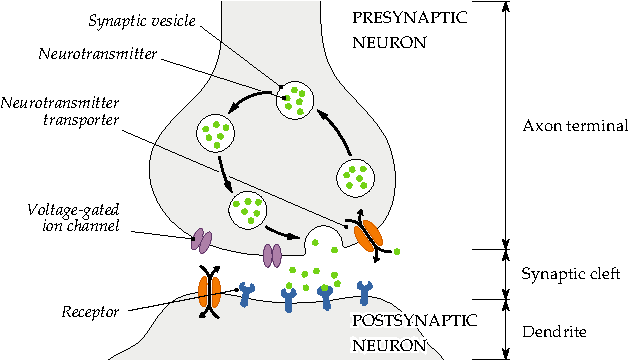
\includegraphics{media/chp2/SynapseSchematic_en.pdf}
	\caption[Chemical synapse schematic]{Chemical synapse, adapted from \url{https://commons.wikimedia.org/wiki/File:SynapseSchematic_en.svg}. See text for description.}
	\label{fig:chemical_synapse}
\end{figure}

As already mentioned in the discussion of artificial neural network models (\cref{sec:neural_network_models}), synapses are the basis for inter-neuron communication and thus neural networks. There are two types of biological synapses: electrical synapses, which allow for a direct exchange of intracellular fluid, and the more common chemical synapses, sketched in \cref{fig:chemical_synapse} and described in the following. If an action potential arrives at the axon terminal of the presynaptic neuron, vesicles containing a neurotransmitter fuse with the cell membrane and release the transmitter into the synaptic cleft. The transmitter then docks onto receptors located at the dendrites of the postsynaptic neuron, where they -- depending on the configuration of the dendritic part of the synapse -- trigger the opening or closing of ion channels and either excite or inhibit the neuron (pull the membrane towards more positive or negative potentials) \cite{kandel2012principles}.

% low-pass filters oder low-pass-filters
Compared to the spike transmission along the axon, the delay occurring at the synapse is rather large. The release of a neurotransmitter furthermore low-pass filters the incoming spikes, stretching their effect over longer time-periods.

\section{Simplified neuron and synapse models}
\label{sec:spiking_neuron_models}

\begin{figure}[t]
	\centering
	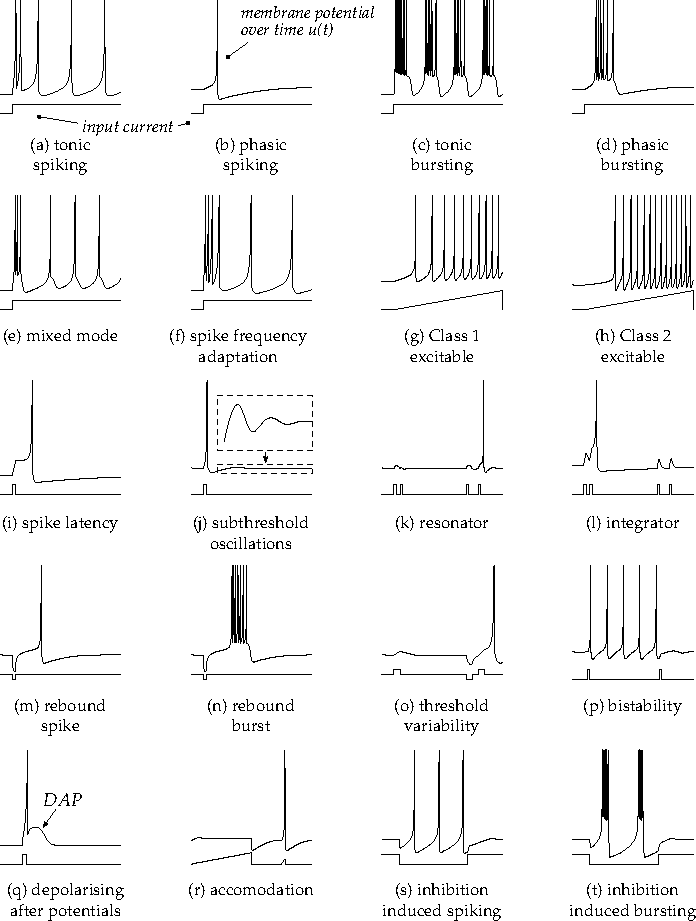
\includegraphics{media/chp2/izhikevich_whichmod_figure1.pdf}
	\caption[Sketches of spiking neuron behavioural patterns]{Sketches of spiking neuron behavioural patterns. Each subgraph shows membrane potential $\um(t)$ and input current $\isyn(t)$ over time. See \cite{izhikevich2004model} for more information. Electronic version of the figure and reproduction permissions are freely available at \url{http://www.izhikevich.com/}.}
	\label{fig:neuron_behaviours}
\end{figure}

The previous sections sketched two extremes: the biophysically meaningful \acrfull{HH} model, and the simplistic firing-rate neuron models used in machine learning. While it is surely possible to use the \HH model as the underlying neuron model for artificial spiking neural networks, its evaluation is computationally expensive \cite{izhikevich2004model} and mathematical analysis is complicated due to its intricate dynamics.

\marginnote{As discussed in \cite{izhikevich2004model}, the \HH model requires up to two magnitudes more floating point operations for the same time\-span as comparably expressive, but simpler models.}
To overcome these limitations, less complex neuron models have been developed. However, their reduced complexity often comes at the cost of reduced expressiveness: \cref{fig:neuron_behaviours} shows the variety of neuron behaviours observed in biological neurons that -- given the correct neuron parameters -- can be described with the \HH model. Yet, the simplest neuron models only support basic modes of operation (\eg \enquote{tonic spiking}). In the remainder of this section we introduce the synapse and neuron models used on the \acrshort{HBP} neuromorphic hardware platforms, list their parameters, and discuss their expressiveness. More information on spiking neuron models can be found in \cite{gerstner2002spiking}.

\subsection{Neuron model base equation}

\marginnote{A summary of the relevant neuron model parameters is given in \vref{tbl:adex_parameters}.}
The representation of the cell membrane as a capacitor with capacitance $\Cm$ is the conceptual basis of most spiking neuron models. Over time the capacitor is charged and discharged by two currents: the intrinsic channel current $\ichan(u, t)$, corresponding to the sum of ionic currents through the ion channels, and the synaptic -- or external -- current $\isyn(\um, t)$ modelling the ionic currents in the synapses as response to external input
\begin{align}
	- \Cm \cdot \dum(t) &= \im(t) = \ichan\left(\um(t), t\right) + \isyn\left(\um(t), t\right) \,.
	\label{eqn:simple_membrane_base_time}
\end{align}
The form of the channel current \ichan depends on the concrete neuron model, whereas the synaptic current \isyn is determined by the synapse model.

\subsection{Synapse models}
\label{sec:synapse_models}

\marginnote{The synapse model is usually independent of the neuron model -- synapses are solely a biologically inspired way to inject a current into a neuron. However, the boundaries will become fuzzy as we introduce excitatory and inhibitory synapses.}
Generally, the synaptic current \isyn is the sum of currents induced by all synapses of a neuron (the number of synapses equals the fan-in of the neuron in the network)
\begin{align}
	\isyn(u, t) &= \sum_{k} \isynk(u, t) \,.
	\label{eqn:synaptic_sum}
\end{align}
The current \isynk caused by each individual synapse $k$ is determined by the internal synapse state. This state is modified whenever the synapse receives a pre-synaptic spike and steadily converges to a resting value. The amplitude of the modification depends on the synapse weight $\wsyn_k$. The physical unit of $\wsyn_k$ depends on the synapse model. Two synapse models are common: \emph{current}-based and \emph{conductance}-based synapses.

\paragraph{Current based synapses with exponential decay}
Synapses of this type do not possess additional state variables -- their sole state is the current \isynk itself. This model is particularly interesting as \isynk does not depend on \um, which in some cases enables fully analytical solutions of the differential in \cref{eqn:simple_membrane_base_time}. Whenever an input spike is received at time $t$, the current is increased by $\wsyn_k$ (in ampere). The synaptic current then exponentially decays to zero over time with time constant $\tau_k$, modelling the low-pass behaviour mentioned in \cref{sec:biological_synapses}. A single current based synapse $k$ can be described as
\begin{align}
	\isynk(t) &\gets \isynk(t) + \wsyn_k \quad \text{on spike for $k$ at } t
	\label{eqn:current_based_sypase} \\
	- \mathrm{d}/\mathrm{d}t \; \tau_k \cdot \isynk(t) &= \isynk(t) \,.
	\label{eqn:current_based_sypase_decay}
\end{align}

\paragraph{Conductance based synapses with exponential decay}
This synapse model is biologically more plausible as it models the transmitter gated membrane channels in biological synapses to a certain extent. As it is available on all neuromorphic hardware platforms, it is the model of choice in this thesis. In contrast to the current based channel, each synapse has a conductance $g_k$ as internal state. An input spike at time $t$ increases the conductance by $\wsyn_k$ (in siemens). As with the current based model, the state variable decays with the synapse-specific time constant $\tau_k$.
\begin{align}
	g_k(t) &\gets g_k(t) + \wsyn_k \quad \text{on spike for $k$ at } t
	\label{eqn:conductance_based_sypase} \\
	- \mathrm{d}/\mathrm{d}t \; \tau_k \cdot g_k(t) &= g_k(t)
	\label{eqn:conductance_based_sypase_decay}
\end{align}
The actual synaptic current \isynk depends on the state $g_k$, the current membrane potential \um and the synaptic channel reversal potential $E_k$.
\begin{align}
	\isynk(\um, t) &= g_k(t) \cdot (\um - E_k)
	\label{eqn:conductance_based_current}
\end{align}
Note that the dependency of \isynk on \um renders finding a closed form solution of the neuron differential equation impossible for any practically useful channel current equation $\ichan(\um, t)$. An example synapse conductivity trace over time with incoming pre-synaptic spikes is shown in \cref{fig:lif_vs_adex}.

\subsection{Excitatory and inhibitory synapses}
\label{sec:excitatory_inhibitory_synapses}

\marginnote{In the software interfaces, the synapse weight \wsyn can be chosen individually per synapse. Usually, positive \wsyn indicate excitatory synapses, negative \wsyn inhibitory synapses (with weight $|\wsyn|$).}
In theory, the reversal potential $E_k$ and time constant $\tau_k$ could be chosen individually for each conductance based synapse. This is biologically implausible, as the reversal potentials are defined by the fixed ion concentration gradients for $\mathrm{K}^+, \mathrm{Na}^+$ and $\mathrm{Cl}^-$. Most simulators -- including the neuromorphic hardware systems -- restrict the number of different synapse types per neuron to two: an excitatory synapse with parameters \Ee, \TauE (corresponding to the $\mathrm{Na}^+$ ion channels), and an inhibitory synapse with parameters \Ei, \TauI (corresponding to the $\mathrm{K}^+$ ion channels).

Usually, the excitatory reversal potential is chosen as $\Ee \geq \ETh$: input spikes that arrive at an excitatory synapse push the membrane potential \um towards the threshold potential \ETh and enable the generation of output spikes. Analogously, the inhibitory synapse reversal potential is chosen as $\Ei \leq \El$, allowing spikes reaching inhibitory synapses to hyperpolarise the neuron.

The restriction of the number of synapse types simplifies the equation for \isyn: two state variables \Ge and \Gi have to be stored per neuron and \isyn can be written as
\begin{align}
	\isyn(\um, t) &= \Ge(t) \cdot (\um - \Ee) + \Gi(t) \cdot (\um - \Ei) \,,
\end{align}
where \Ge or \Gi are adapted according to \cref{eqn:conductance_based_sypase} for input spikes reaching excitatory/inhibitory synapses. The conductances decay with time constants \TauE and \TauI as described in \cref{eqn:conductance_based_sypase_decay}.

\subsection{Linear integrate-and-fire neuron model}
\label{sec:lif}

The \LIF neuron model can be seen as a minimal extension of \cref{eqn:simple_membrane_base_time}: the simulated neuron membrane contains a leak channel with constant conductance \Gl, pulling the membrane towards the resting potential \El. For excitatory and inhibitory synapses as described in \cref{sec:excitatory_inhibitory_synapses}, the differential equation for the membrane potential $\um(t)$ is given as
\begin{align}
	- \Cm \cdot \dum(t) &= \Gl \cdot (\um(t) - \El) + \isyn(u(t), t) \label{eqn:lif} \\
		&= \Gl \cdot (\um(t) - \El) + \Ge(t) \cdot (\um(t) - \Ee) + \Gi(t) \cdot (\um(t) - \Ei) \notag \,.
\end{align}
\marginnote{The output action potential is not explicitly formed as a spike in the \LIF model. For visualisation purposes a spike reaching up to a potential $\Espike$ is often artificially inserted at the threshold-crossing.}
The above equation does not account for spike generation and refractoriness of the neuron. An output spike is generated, whenever the membrane potential $\um(t)$ crosses a certain threshold $\ETh > \El$. The refractory period is modelled by tracking the last output spike time $t_{\mathrm{spike}}$ (initialised with $-\infty$). While the condition $t - t_\mathrm{spike} \leq \TauRef$ holds, the membrane potential is clamped to the reset potential $\Ereset \leq \El$
\begin{align}
	t_\mathrm{spike} &\gets t &&\text{if } & \um(t) &\geq \ETh \\
	\um(t) &\gets \Ereset &&\text{while } & t - t_\mathrm{spike} &\leq \TauRef \,.
	\label{eqn:lif_reset}
\end{align}

The expressiveness of this model is severely limited: given a constant input current $\isyn(t)$, the model can only operate in the tonic spiking mode (\cref{fig:neuron_behaviours}). All state information is lost once an output spike is issued and the membrane potential is reset \cite{izhikevich2004model}.

More complex behaviour such as bursting can only be realised in conjunction with the synapse model. In combination with conductance based synapses, the \LIF model is also referred to as \acrshort{IfCondExp} model. Despite its shortcomings the model is extensively used in spiking neural network simulations. Furthermore, it is supported by all neuromorphic hardware platforms in the \acrfull{HBP}.

\subsection{Non-linear integrate-and-fire models}
\label{sec:nlif}

\begin{figure}
	\small
	\centering
	\subbottom[LIF model]{%
		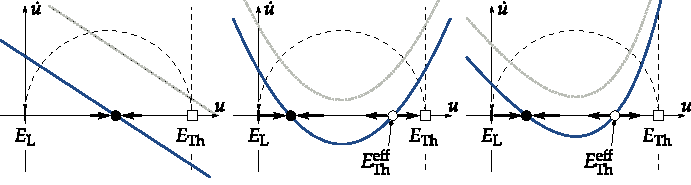
\includegraphics[trim=0cm 0cm 7.8cm 0cm,clip]{media/chp2/neuron_state_space.pdf}%
		\label{fig:lif_state}%
	}%
	\subbottom[QIF model]{%
		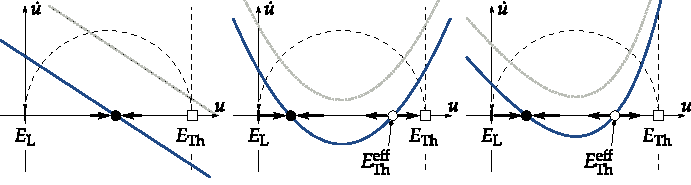
\includegraphics[trim=3.9cm 0cm 3.9cm 0cm,clip]{media/chp2/neuron_state_space.pdf}%
		\label{fig:qif_state}%
	}
	\subbottom[EIF model]{%
		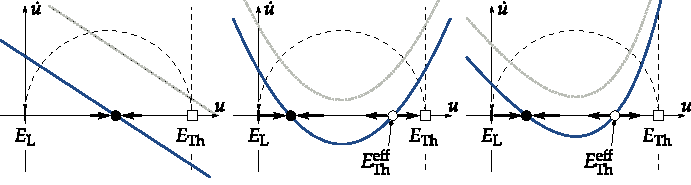
\includegraphics[trim=7.8cm 0cm 0cm 0cm,clip]{media/chp2/neuron_state_space.pdf}%
		\label{fig:eif_state}%
	}
	\caption[One dimensional integrate-and-fire model bifurcation patterns]{Sketch of one dimensional integrate-and-fire model bifurcation patterns. The three graphs show $\dum(\um)$ and the stationary points $\dum(\um) = 0$ for non-zero $\isyn$. Filled circles indicate stable stationary points, unfilled circles unstable stationary points. The reset mechanism is indicated by the unfilled box at $\um = \ETh$ and the dashed arrow pointing back at $\um$. The dotted grey lines show the same graph with a different choice for \isyn. Inspired by \cite{izhikevich2007dynamical}.}
	\label{fig:nlif_state}
\end{figure}

The \LIF neuron model has a severe instability in its dynamics: for $\El < \um < \ETh$, given $\isyn=0$, the differential $\dum(\um)$ in \cref{eqn:lif} evaluates to $\dum(\um) < 0$, even for infinitesimally small $\ETh - \um$. As shown in \cref{fig:lif_state}, it is only once \um reaches \ETh that an output \enquote{spike} is issued and the neuron is reset.

This behaviour has two major shortcomings. The model does not produce a sharp spike-formed action potential with a sudden rise in the membrane potential, and the biological phenomenon of \emph{spike latency} (\cref{fig:neuron_behaviours}(i), \cite{izhikevich2004model}) is not modelled: for a single short input current pulse the neuron might not spike immediately, but with a certain delay that decreases with the amplitude of the pulse.

\marginnote{The inner term in $f$ merely shifts and rescales the membrane potential \um, such that $\El$ maps to a dimensionless $0$ and $\ETh$ to $1$ (before $\El$ is subtracted).}
Spike generation and spike latency are modelled by non-linear integrate-and-fire neurons
\begin{align}
	- \Cm \cdot \dum(t) &= \Gl \cdot \left( f\left(\frac{\um(t) - 2 \cdot \El}{\ETh - \El}\right) \cdot (\ETh - \El) + \El \right) + \isyn
	\label{eqn:nlif} \,,
\end{align}
where $f$ is some non-linear function. If $f$ is chosen as the identity function, \cref{eqn:lif,eqn:nlif} are equivalent.

Examples for non-linear integrate-and-fire models are the \QIF and \EIF models: the corresponding functions $f$ with free parameters $f_1$, $f_2$ are given as
\begin{align}
	f_{\mathrm{QIF}}(u) &= - f_1 \cdot (u - f_2)^2
	& f_{\mathrm{EIF}}(u) &= u - f_1 \cdot \exp(u - f_2) \,.
	\label{eqn:nlif_f}
\end{align}
\marginnote{Care has to be taken when performing numerical integration of the equation, as the non-linearity might be numerically unstable.}
As shown in \cref{fig:qif_state,fig:eif_state} the behaviour of these two models is qualitatively equivalent: as soon as \um crosses a certain value \EThEff, the potential is quickly pushed towards \ETh. Analogously to the \LIF model, for $\um < \EThEff$ the membrane converges towards a stable stationary point. Location and existence of the two stationary points depends on the external input current \isyn.

\subsection{Two-dimensional Hodgkin-Huxley approximations: the AdEx model}
\label{sec:adex}

The above integrate-and-fire neuron models are one-\-dim\-en\-sio\-nal: their state vector solely consists of the membrane potential \um. As mentioned at the end of \cref{sec:lif}, one-dimensional models cannot account for many of the observed behavioural patterns in biological neurons, as the neuron state \um is reset along with each output spike. Surprisingly, most of the relevant behaviour of the \HH model (which has four state variables) can be modelled with only two-dimensions.

The Izhikevich model is a well-established and computationally cheap example of such an approximation \cite{izhikevich2004model}. Another interesting approximation is the \MAT model, which minimally extends the \LIF model with an adaptive threshold $\ETh(t)$. Due to its linearity, the model is numerically stable and yet very successful in approximating membrane potential traces recorded from biological neurons \cite{kobayashi2009made}.

\marginnote{The adaptation current $\iadap(t)$ can be biologically interpreted as a form of habituation or short-time plasticity \cite{kandel2012principles}.}
In this thesis we focus on the \AdEx model implemented in hardware in the \HBP physical model system \acrshort{NMPM}. Just as the above models, it is a two-dimensional non-linear integrate-and-fire model which reproduces a majority of the behavioural patterns observed in nature \cite{AdExp2005,AdExpScholarpedia2009}. In addition to the membrane potential $\um(t)$, the \AdEx model tracks an adaptation current $\iadap(t)$, which hyperpolarises the neuron. The current $\iadap(t)$ increases by a small constant $\ib$ with every generated output spike
\begin{align}
	\iadap(t) &\gets \iadap(t) + \ib \quad \text{on } \um(t) > \ETh \,.
	\label{eqn:adex_iadap}
\end{align}
\marginnote{The subthreshold adaptation allows to model the biological phenomenon of \enquote{threshold variability}, see \cref{fig:neuron_behaviours}(o).}
The adaptation current \iadap decays exponentially with a time constant \TauA and additionally depends on the \enquote{subthreshold adaptation conductance} $\Ga \geq 0$ which controls the influence of the membrane potential on the decay rate. For $\um(t) < \El$ the adaptation current decays faster, while $\um(t) > \El$ prolongs the decay:
\begin{align}
 	- \mathrm{d}/\mathrm{d}t \; \TauA \cdot \iadap(t) &= \iadap(t) - \Ga \cdot (\um(t) - \El) \,. \label{eqn:adex_tauA}
\end{align}

\marginnote{In the original \AdEx paper and corresponding code, \EThExp is usually referred to as \ETh, and \ETh is replaced by a potential \Espike.}
The model furthermore inherits the exponential spike generation mechanism from the \EIF model as described in \cref{eqn:nlif,eqn:nlif_f}. The final model equation is given as
\begin{align}
	\hspace{-0.2cm}-\Cm \cdot \dum(t) &= \Gl \cdot (\um(t) - \El) + \ITh(\um(t)) + \iadap(t) + \isyn(\um(t), t) \label{eqn:adex} \\
	\ITh(\um) &= \Gl \cdot \DT \cdot \exp \left(\frac{\um - \EThExp}{\DT}\right) \,.
	\label{eqn:adex_ith}
\end{align}
The exponential threshold potential \EThExp controls the minimum membrane potential $\um(t)$ at which the inner term of the exponential in $\ITh(u)$ is positive. For larger membrane potentials an exponentially rising current triggers an avalanche which causes the generation of an output spike. The parameter \DT controls the slope of the exponential current. While the rising spike onset is explicitly modelled, the falling edge is not. The same reset mechanism as in the \LIF model in \cref{eqn:lif_reset} is used, albeit the reset threshold \ETh is chosen considerably larger in the \AdEx model.


\begin{figure}
	\centering
	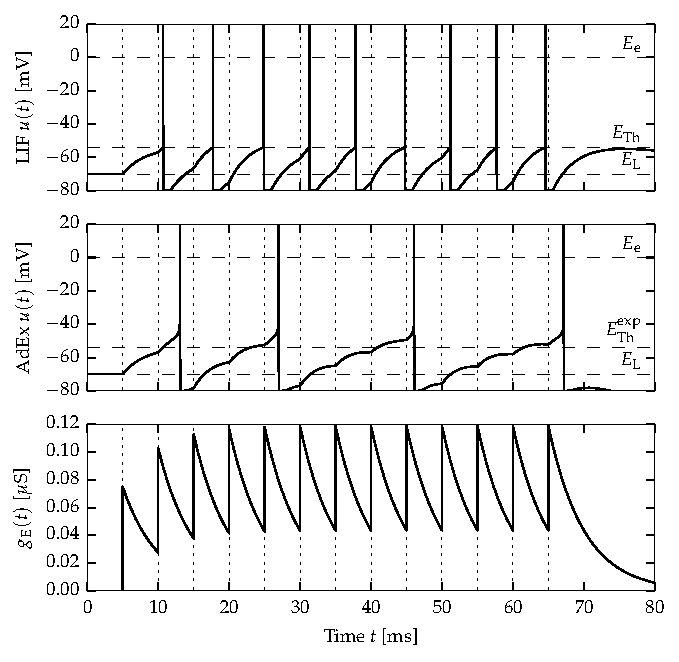
\includegraphics{media/chp2/lif_vs_adex.pdf}
	\caption[Comparison between the LIF and AdEx neuron models]{Comparison between the \LIF and \AdEx neuron models. The first two plots show the membrane potential of a \LIF and an \AdEx neuron, the bottom plot the conductance of a conductance based excitatory synapse, which receives 13 spikes in an interval of $\isi = \SI{5}{\milli\second}$. Due to the adaptation current, the output spike rate of the \AdEx neuron decreases over time, whereas the \LIF neuron outputs spikes at a constant rate. The spike potential at $\Espike = \SI{20}{\milli\volt}$ is artificially inserted by the simulator for the \LIF model, the \AdEx model intrinsically generates a spike onset.}
	\label{fig:lif_vs_adex}
\end{figure}

\cref{fig:lif_vs_adex} depicts a comparison of the behaviour of a \LIF and an \AdEx neuron with a conductance based synapse for a series of input spikes with equidistant timing. As a result of the adaptation current the output spike rate reduces over time.

\begin{table}
	\centering
	\small
	\newcommand{\SA}{\ensuremath{\circ}}
	\newcommand{\SB}{\ensuremath{\diamond}}
	\vspace*{0.45cm}
	\begin{tabular}{c l p{5.65cm} r r l}
		\toprule
		\multicolumn{6}{c}{\spacedlowsmallcaps{LIF and AdEx model parameters and typical values}} \\
		\midrule
		\multicolumn{6}{c}{\slshape Potentials} \\
		\midrule

			& & \spacedlowsmallcaps{Description} & \spacedlowsmallcaps{LIF} & \spacedlowsmallcaps{AdEx} & \\

			\noalign{\vskip 2mm}
			& \El  & Membrane leak or resting potential
			& $-65.0$ & $-70.6$ & [\si{\milli\volt}]\\

			\noalign{\vskip 2mm}
			& \ETh & Threshold potential. If passed, the neuron resets and issues an output spike.
 			& $-50.0$ & $-40.0$ & [\si{\milli\volt}] \\

			\noalign{\vskip 2mm}
			& \Ereset & Reset potential. Potential the membrane is reset to during the refractory period.
			& $-65.0$ & $-70.6$ & [\si{\milli\volt}] \\

			\noalign{\vskip 2mm}
		\SB & \Ee & Excitatory synapse reversal potential
			& $0.0$ & $0.0$ & [\si{\milli\volt}] \\

			\noalign{\vskip 2mm}
		\SB & \Ei & Inhibitory synapse reversal potential
			& $-70.0$ & $-80.0$ & [\si{\milli\volt}] \\

		\midrule
		\multicolumn{6}{c}{\slshape Time constants} \\
		\midrule

			& & \spacedlowsmallcaps{Description} & \spacedlowsmallcaps{LIF} & \spacedlowsmallcaps{AdEx} & \\

			\noalign{\vskip 2mm}
			& \TauRef & Duration of the refractory state
			& $0.1$ & $0.1$ & [\si{\milli\second}] \\

			\noalign{\vskip 2mm}
		\SB & \TauE & Excitatory synapse time constant
			& $5.0$ & $5.0$ & [\si{\milli\second}] \\

			\noalign{\vskip 2mm}
		\SB & \TauI & Inhibitory synapse time constant
			& $5.0$ & $5.0$ & [\si{\milli\second}] \\

		\midrule
		\multicolumn{6}{c}{\slshape Membrane parameters} \\
		\midrule

			& & \spacedlowsmallcaps{Description} & \spacedlowsmallcaps{LIF} & \spacedlowsmallcaps{AdEx} & \\

			\noalign{\vskip 2mm}
			& \Cm & Membrane capacitance
			& $1.0$ & $0.281$ & [\si{\nano\farad}] \\

			\noalign{\vskip 2mm}
			& \Gl & Membrane leak conductance
			& $0.05$ & $0.03$ & [\si{\micro\siemens}] \\

			\noalign{\vskip 2mm}
			& \TauM & Membrane time constant\newline ($\TauM = \Cm / \Gl$ )
			& $20.0$ & $9.37$ & [\si{\milli\second}] \\

		\midrule
		\multicolumn{6}{c}{\slshape AdEx adaptation and exponential current mechanism} \\
		\midrule

			& & \spacedlowsmallcaps{Description} & \spacedlowsmallcaps{LIF} & \spacedlowsmallcaps{AdEx} & \\

			\noalign{\vskip 2mm}
 		\SA & \Ga & Subthreshold adaptation
			& / & $4.0$ & [\si{\nano\siemens}] \\

			\noalign{\vskip 2mm}
		\SA & \ib & Spike-triggered adaptation current
			& / & $0.08$ & [\si{\nano\ampere}] \\

			\noalign{\vskip 2mm}
		\SA & \TauA & Adaptation current time constant
			& / & $144.0$ & [\si{\milli\second}] \\

			\noalign{\vskip 2mm}
		\SA & \EThExp & Exponential threshold potential
			& / & $-50.4$ & [\si{\milli\volt}] \\

			\noalign{\vskip 2mm}
		\SA & \DT & Exponential current slope
			& / & $2.0$ & [\si{\milli\volt}] \\

		\midrule
		\multicolumn{6}{c}{\slshape State variables} \\
		\midrule

			& & \spacedlowsmallcaps{Description} & \spacedlowsmallcaps{LIF} & \spacedlowsmallcaps{AdEx} & \\

			\noalign{\vskip 2mm}
			& $\um(t)$ & Membrane potential & / & / & [\si{\volt}] \\

			\noalign{\vskip 2mm}
		\SA & $\iadap(t)$ & Adaptation current & / & / & [\si{\ampere}] \\

			\noalign{\vskip 2mm}
		\SB & $\Ge(t)$ & Excitatory channel conductance & / & / & [\si{\siemens}] \\

			\noalign{\vskip 2mm}
		\SB & $\Gi(t)$ & Inhibitory channel conductance & / & / & [\si{\siemens}] \\
		\bottomrule
	\end{tabular}
	\caption[LIF and AdEx model parameters and state variables]{Parameters of the \LIF and \AdEx neuron models and state variables in conjunction with excitatory and inhibitory conductance based synapses. The typical values reflect the biologically motivated default parameters in \PyNN~0.8. \SA\ Only available in the AdExp model. \SB\ Synapse parameters.}
	\label{tbl:adex_parameters}
\end{table}
The \AdEx model can emulate the simpler \LIF model by setting the parameters \Ga and \ib to zero and deactivating the exponential threshold current \ITh, which -- depending on the implementation -- can be achieved by setting \DT to zero. \cref{tbl:adex_parameters} gives an overview of all parameters in the \AdEx and \LIF model with conductance based excitatory and inhibitory synapses.

\section{Neuromorphic hardware}
\label{sec:neuromorphic_hardware}

Biological spiking neural networks, including the human brain, are asynchronous, distributed, extremely parallel and stochastic. Classical digital computers on the other hand are synchronous, centralised, of limited parallelism and deterministic. They are conceivably ill-suited for time and energy efficient simulation of large-scale spiking neural networks. The term \emph{neuromorphic hardware} refers to systems which trade the versatility of general purpose computers with the architectural properties of central nervous systems and are specifically developed for a certain range of neural network models. Neural networks have been predominantly implemented in hardware in the 1950s and 1960s, when no powerful general purpose computers were available, see for example \cite{hay1960mark,widrow1960adaptive}. However, no system for brain-scale networks has been developed to date.

\marginnote{The description of the hardware systems in this chapter follows their specification, comments regarding the current state of the systems at the time of writing are given in \cref{chp:experiments}.}
Providing such neuromorphic hardware platforms is a central aim of the \HBP. Here, two complementary approaches are pursued. The physical model \acrshort{NMPM} simulates individual neurons and synapses as analogue physical model circuits. Conversely, the fully digital many-core system \acrshort{NMMC} consists of a vast number of conventional microprocessors, each of which simulates a small number of neurons. In both systems spikes are propagated over a digital, packet based, asynchronous and potentially unreliable communication network \cite{hbp_neuromorphic_platform}. In this section we describe \NMMC, \NMPM, its single-chip predecessor \enquote{Spikey} and the software stack provided to the end-user.

\subsection{NM-MC1: The many-core system}

The neuromorphic many-core system \NMMC is developed at the University of Manchester and based on the SpiNNaker chip, a multiprocessor designed for real-time simulation of spiking neural networks \cite{hbp_neuromorphic_platform}. Each chip contains up to 18 ARM968 processors running at a nominal frequency of $\SI{180}{\mega\hertz}$, with one processor dedicated to management purposes. Each processor has access to $32\,\mathrm{KiB}$ of instruction memory and $64\,\mathrm{KiB}$ data memory, while each chip connects to $128\,\mathrm{MiB}$ of external DDR SDRAM. Additionally, SpiNNaker features six bidirectional inter-chip communication links with integrated router used to exchange spike events over the network of chips during simulation. \NMMC consists of boards with 48 SpiNNaker chips each, organised in a torus network topology. \NMMC will eventually consist of ten cabinets with 120 boards each, resulting in a maximum of $979\,200$ processors for neural network simulation \cite{painkras2013spinnaker,furber2013overview}.

The system is theoretically capable of running any neuron model. However, the processors do not feature a floating-point unit, so in order to avoid the overhead of a software floating-point implementation, the neuron time dynamics are simulated with fixed-point arithmetic. As \mbox{\NMMC} is designed for the execution of spiking neural networks at biological timescale, the number of neurons per core varies with the computational complexity of the model. The system supports the \LIF model with both conductance and current based synapses, as well as the Izhikevich neuron model \cite{hbp_neuromorphic_platform, izhikevich2004model}. Algorithmically, the \LIF neuron dynamics are integrated using the Euler method at \SI{1}{\milli\second} timestep with 32-bit intermediate fixed-point values and 16-bit fixed-point parameter storage, allowing up to 256 \LIF neurons with conductance based synapses in a single core \cite{rast2010leaky}. Correspondingly, \NMMC can simulate up to 250 million neurons, which is two orders of magnitude smaller than the estimated number of neurons in the human cortex \cite{braitenberg2013cortex}.

\subsection{NM-PM1: The physical model}

\begin{figure}
	\centering
	\vspace*{0.4cm}
	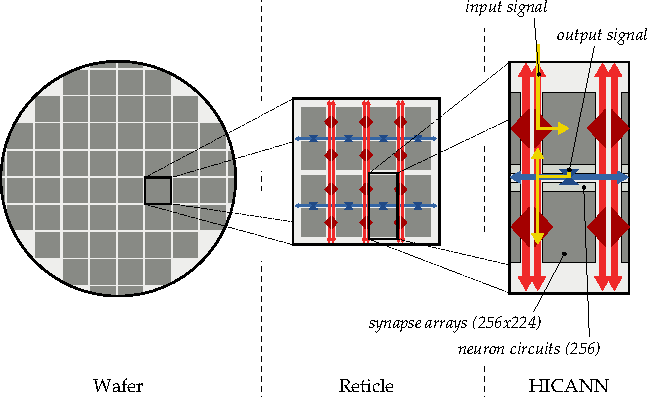
\includegraphics{media/chp2/nmpm1_sketch.pdf}\\
	\vspace*{0.4cm}
	\caption[NM-PM1 wafer high level architecture overview]{\NMPM wafer high level architecture overview. A single wafer in the NM-PM1 system consists of 384 \HICANN chips, organised in reticles. A \HICANN consists of two analogue blocks, each built of a synapse array and a neuron circuit. Each \HICANN is connected to an on-chip network, organised in horizontal buses (blue) receiving neuron output, and vertical buses (red) transmitting input signals to the synapse drivers. Adapted from \cite{petrovici2014characterization}.}
	\label{fig:nmpm1_sketch}
\end{figure}

\marginnote{Research on \HICANN and \NMPM originated in the European \FACETS and \BrainScaleS projects and is now continued in the \HBP.}
The neuromorphic physical model \NMPM is developed at the Kirchhoff Institute for Physics at Heidelberg University. \NMPM is built around the mixed-signal \HICANN (\acrlong{HICANN}) chip. Each \HICANN consists of two blocks, each hosting 256 analogue neuron circuits and a $224\times256$ matrix of analogue synapse circuits. Adjacent rows in the synapse matrix receive external input via synapse drivers (112 per block), which are connected to a digital on-chip communication network. To provide neurons with variable synapse count, up to 64 physical neuron circuits can be joined to form a logical neuron, allowing up to $14\,336$ synapses per logical neuron at the cost of reducing the number of logical neurons per block to a minimum of four. Each synapse can store a 4-bit weight. Synapse rows can be combined in order to achieve a higher weight resolution.

The analogue circuits on the chip emulate the dynamics of the \AdEx and \LIF models with excitatory and inhibitory conductance based synapses. Due to the analogue implementation it is important to distinguish model and hardware parameters: individual hardware parameters are mostly configured as voltages in analogue floating gates. The biological model parameters must be mapped onto these hardware parameters, taking calibration values for the individual circuits into account.
\marginnote{Alternatively, the speedup factor can specified by the user, but then only limited choices regarding the membrane capacitance \Cm are possible.}
As each neuron circuit can only be configured to use one of two membrane capacitances, the mapping process must not only adapt the model membrane potentials, currents, and conductivities to their hardware voltage representation, but also rescale the time constants to match the model membrane capacitance $\Cm$. This results in a speedup factor between $10^3$ and $10^5$ compared to biological timescale.

Apart from the $10^5$ speedup factor, another salient property of \NMPM is its wafer-scale integration: instead of separating the individual \HICANN chips from their silicon wafer after manufacturing, the wafer is left intact. Connections between the largest lithographic units -- the reticles -- are layered onto the wafer in a post-processing step. The wafer-scale approach is feasible, as errors in the analogue circuitry are tolerable (as they are in biological systems) and can be marked
\marginnote{While impressive, the number of neurons in \NMPM is still four magnitudes smaller than the estimated number of neurons in the human brain, but already close to the size of a mouse cortex \cite{braitenberg2013cortex}.}
as such in software. Each wafer comprises 384 {\HICANN}s, summing up to a theoretical maximum of $1\,966\,080$ neurons and $44$ million synapses \cite{petrovici2014characterization}. An overview of the organisational topology is depicted in \cref{fig:nmpm1_sketch}. In its final stage, \NMPM is planned to consist of 20 wafer systems, resulting in a total of $3.9$ million neurons \cite{hbp_neuromorphic_platform}. The \ESS allows to simulate parts of \NMPM without access to the actual hardware \cite{bruderle2011comprehensive}.

\subsection{Spikey}
\label{sec:spikey}

The Spikey analogue neuromorphic hardware system (\cref{fig:spikey}) has been developed as part of the \FACETS project at the University of Heidelberg. As a predecessor to \HICANN, the single Spikey chip in the system offers a speedup factor of $10\,000$ compared to biological timescale, and 384 analogue neurons, split into two blocks of 192 neurons each.
Each neuron implements a limited \LIF model and connects to 256 configurable analogue synapses with 4-bit weight resolution. Synapses are organised in 256 lines per block, with each line passing inputs from external or internal sources to the synapses. The neuron parameters \TauRef and \Gl can be chosen per neuron, all other neuron parameters are shared by groups of 96 neurons \cite{pfeil2013six}.

\subsection{Software stack}
\label{sec:pynn}

\begin{figure}
	\centering
	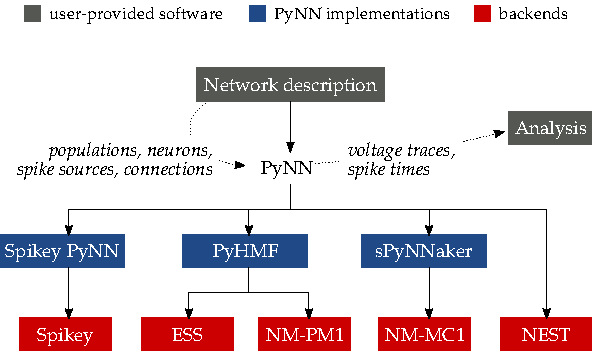
\includegraphics{media/chp2/pynn_software_stack.pdf}\\
	\caption[Neuromorphic hardware system software stack and data flow]{Neuromorphic hardware system software stack and data flow. Users provide a network description to \PyNN and request the recording of certain variables. Implementations of the \PyNN \acrshort{API} (blue) then communicate with the backend specific software (red). An interface for \NEST is directly included in \PyNN.}
	\label{fig:pynn_software_stack}
\end{figure}

Usually, neuromorphic hardware platforms, their emulators, and software simulators come with a native software interface specifically tailored to the system. For neuromorphic hardware, the backends map the network graph onto the neuromorphic substrate (place-and-route), convert the abstract neuron model parameters to concrete hardware parameters and perform the necessary communication tasks.

While the platform-provided libraries allow users to exploit specific platform features, their variety hinders the development of cross-platform network simulations, as each platform has to be targeted individually. To overcome this limitation, an \API with the name \PyNN is developed as part of \HBP \cite{davison2008pynn}. As shown in \cref{fig:pynn_software_stack}, \PyNN specifies a common software interface that allows to construct spiking neural network graphs, inject spike sources and flag neuron spike times and membrane potentials for recording. The individual developers of the hardware or software simulators provide an implementation of the \PyNN interface that communicates with the corresponding backend. This allows code written on top the \PyNN framework to run on arbitrary platforms, as long as it provides the required neuron models and the parameters are in the supported range.

Platforms targeted in this thesis via \PyNN are Spikey, \NMPM and its emulation \ESS, \NMMC and the software simulator \NEST. \NEST is developed at the Forschungszentrum Jülich as part of the research on large scale simulation of brain models on conventional high performance computing platforms in the \HBP \cite{gewaltig2007nest}. By design, \NEST is the most versatile and mathematically exact of the targeted platforms and acts as a reference system in this thesis.


%
% BINAM
%

\section{The Willshaw associative memory model (BiNAM)}
\label{sec:willshaw_theory}

\begin{figure}
	\footnotesize
	\centering
	\newlength{\tilewidth}
	\setlength{\tilewidth}{0.184\textwidth}
	\setlength{\tabcolsep}{2.75pt}
	\begin{tabular}{c c c c c}%
		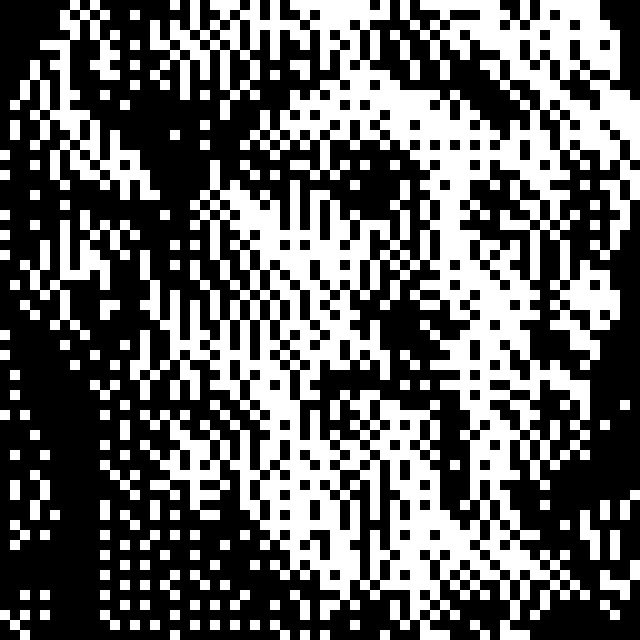
\includegraphics[width=\tilewidth,interpolate=false]{media/chp2/associative_memory/hopfield/04_00_orig_scaled_crushed.png}&%
		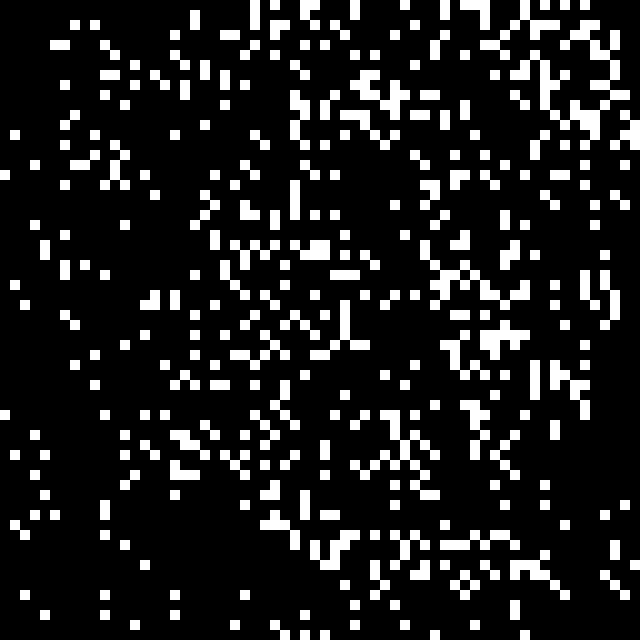
\includegraphics[width=\tilewidth,interpolate=false]{media/chp2/associative_memory/hopfield/04_01_noise_scaled_crushed.png}&%
		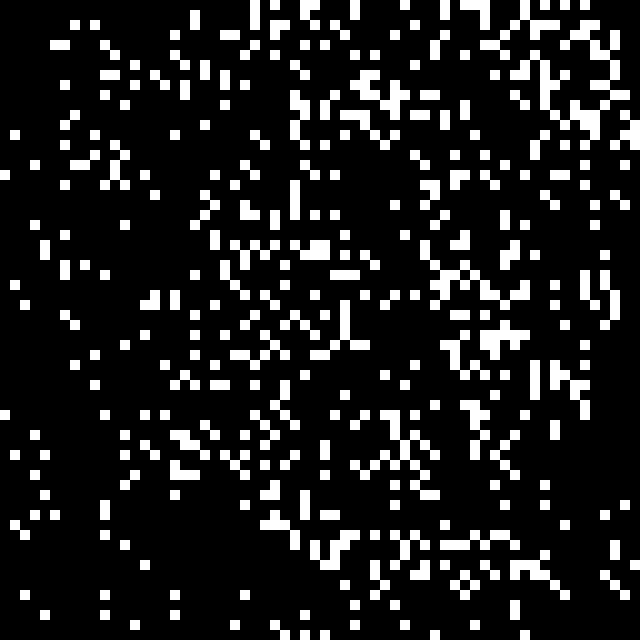
\includegraphics[width=\tilewidth,interpolate=false]{media/chp2/associative_memory/hopfield/04_02_activation_scaled_crushed.png}&%
		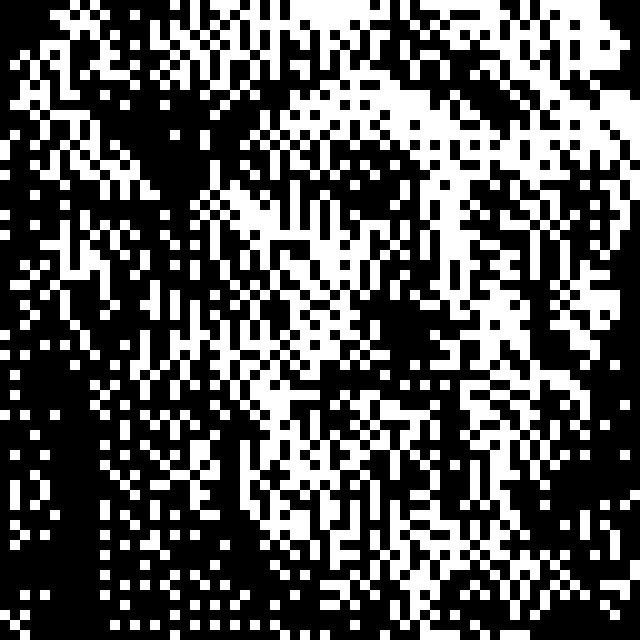
\includegraphics[width=\tilewidth,interpolate=false]{media/chp2/associative_memory/hopfield/04_03_activation_scaled_crushed.png}&%
		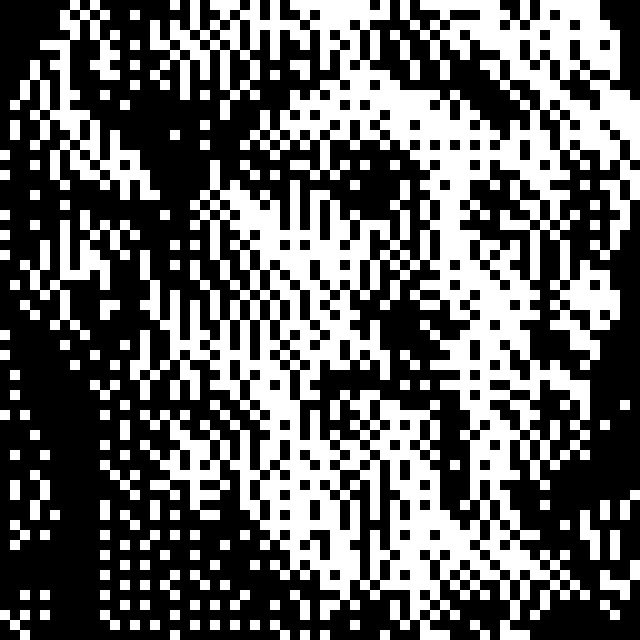
\includegraphics[width=\tilewidth,interpolate=false]{media/chp2/associative_memory/hopfield/04_04_activation_scaled_crushed.png}\\%
		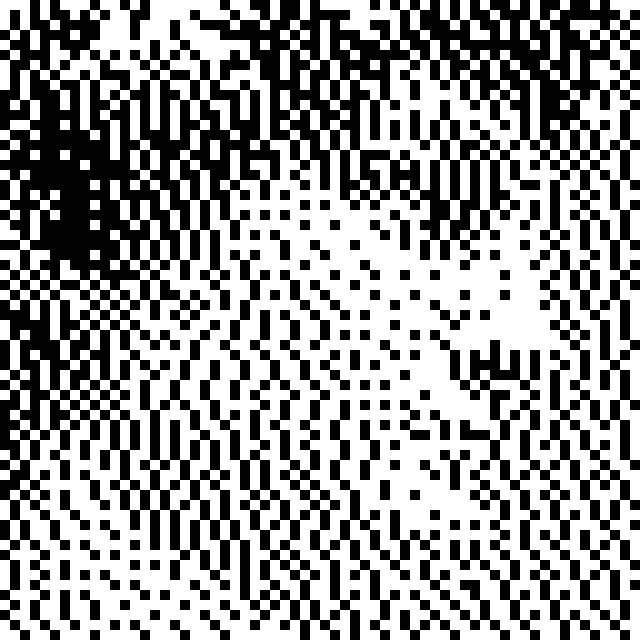
\includegraphics[width=\tilewidth,interpolate=false]{media/chp2/associative_memory/hopfield/05_00_orig_scaled_crushed.png}&%
		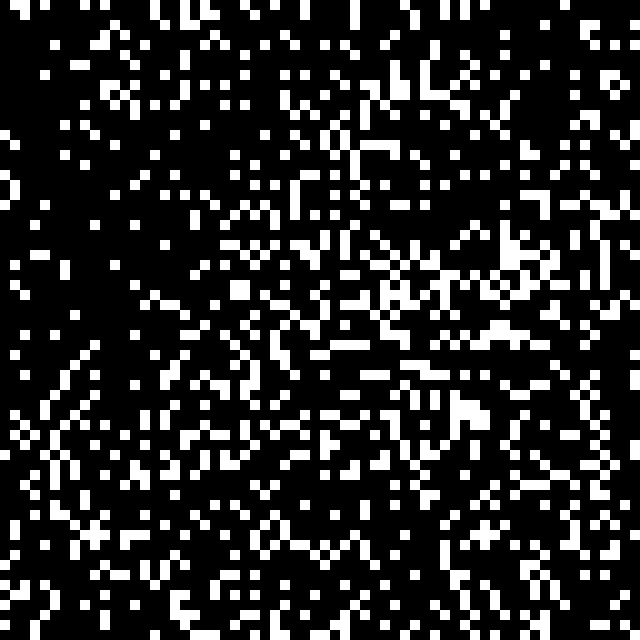
\includegraphics[width=\tilewidth,interpolate=false]{media/chp2/associative_memory/hopfield/05_01_noise_scaled_crushed.png}&%
		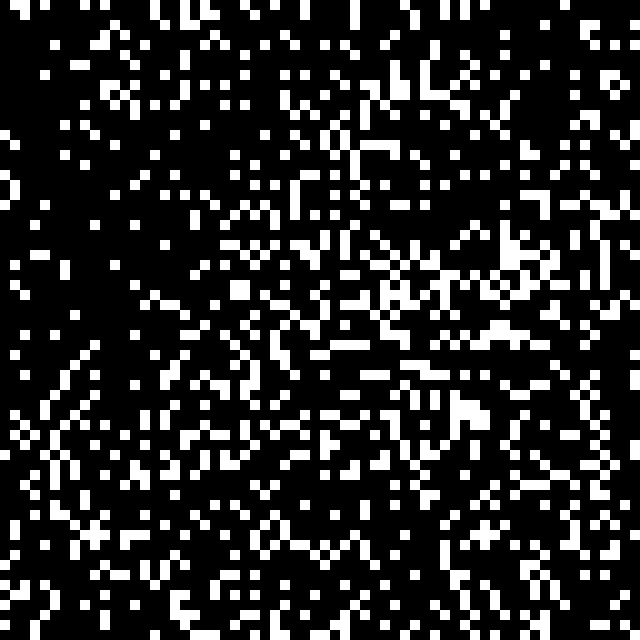
\includegraphics[width=\tilewidth,interpolate=false]{media/chp2/associative_memory/hopfield/05_02_activation_scaled_crushed.png}&%
		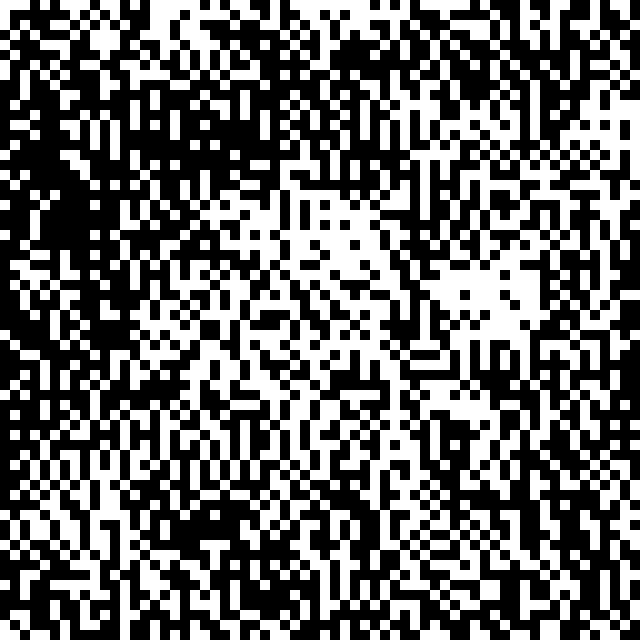
\includegraphics[width=\tilewidth,interpolate=false]{media/chp2/associative_memory/hopfield/05_03_activation_scaled_crushed.png}&%
		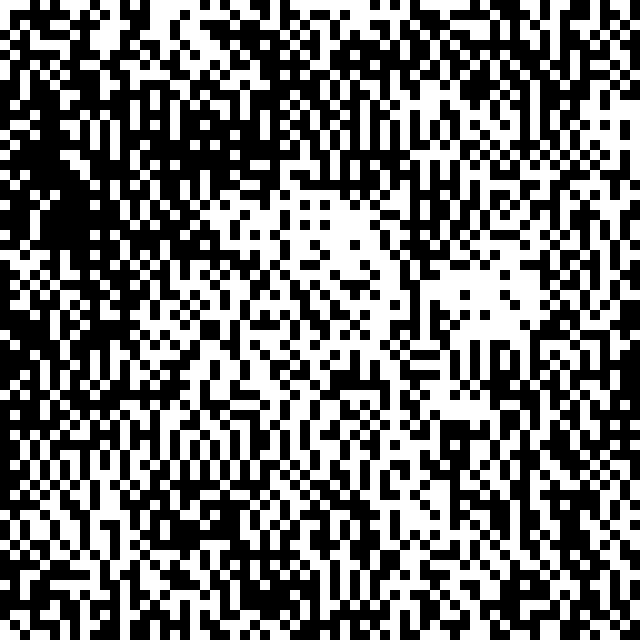
\includegraphics[width=\tilewidth,interpolate=false]{media/chp2/associative_memory/hopfield/05_04_activation_scaled_crushed.png}\\%
		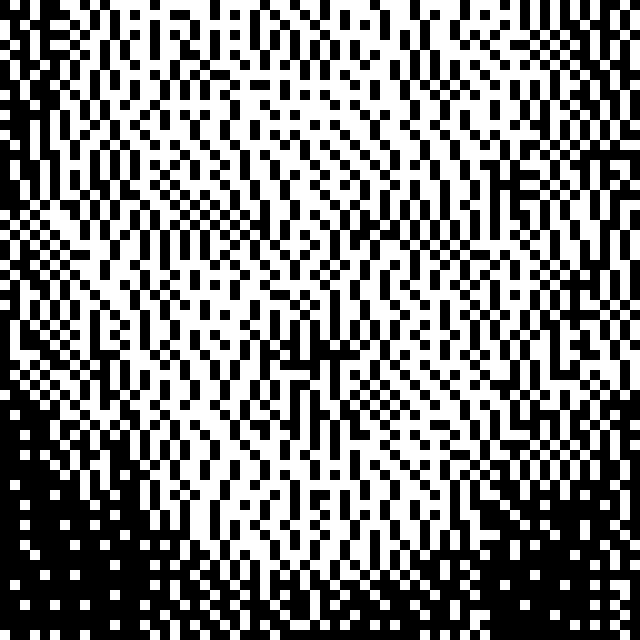
\includegraphics[width=\tilewidth,interpolate=false]{media/chp2/associative_memory/hopfield/06_00_orig_scaled_crushed.png}&%
		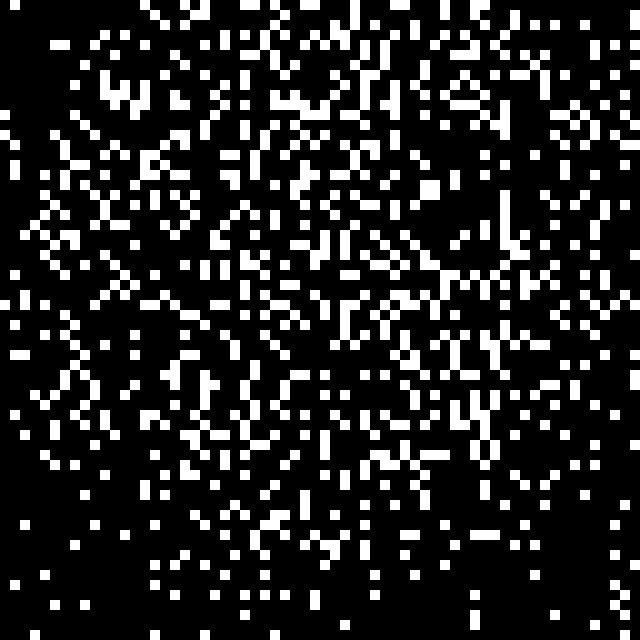
\includegraphics[width=\tilewidth,interpolate=false]{media/chp2/associative_memory/hopfield/06_01_noise_scaled_crushed.png}&%
		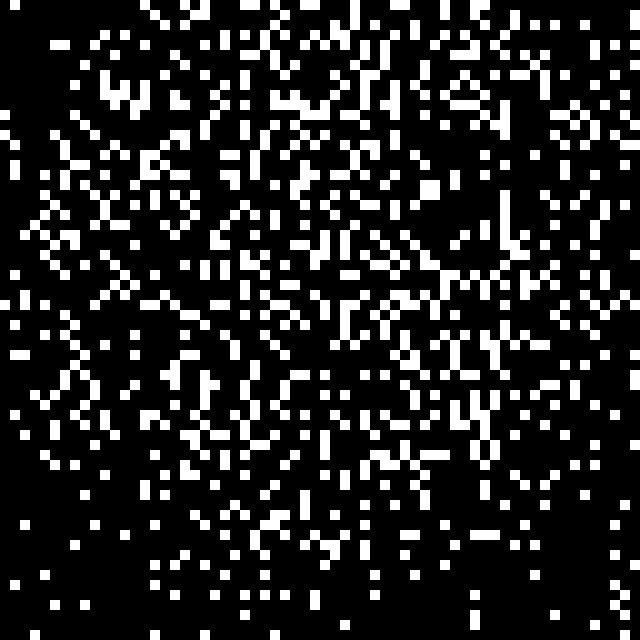
\includegraphics[width=\tilewidth,interpolate=false]{media/chp2/associative_memory/hopfield/06_02_activation_scaled_crushed.png}&%
		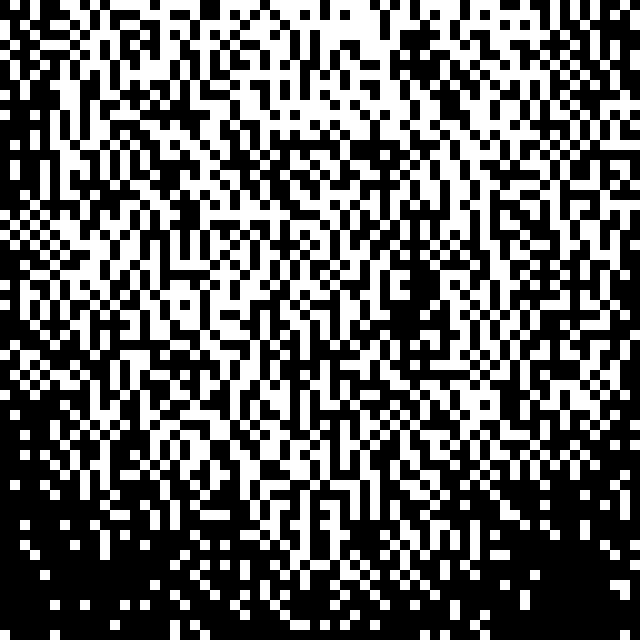
\includegraphics[width=\tilewidth,interpolate=false]{media/chp2/associative_memory/hopfield/06_03_activation_scaled_crushed.png}&%
		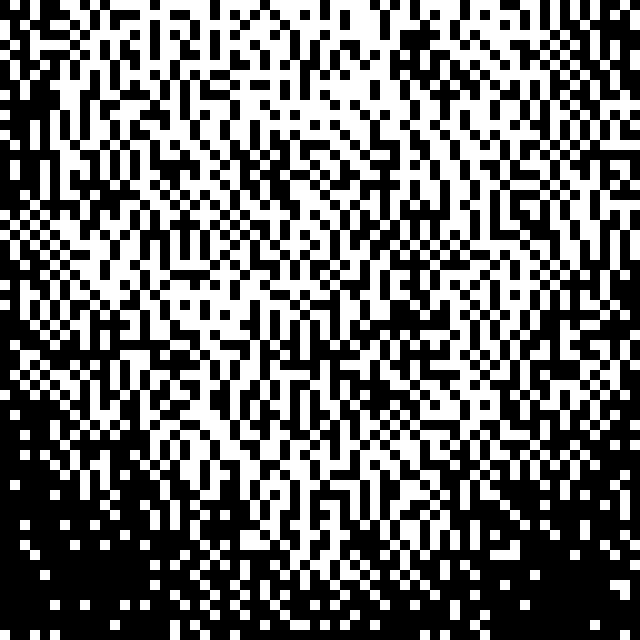
\includegraphics[width=\tilewidth,interpolate=false]{media/chp2/associative_memory/hopfield/06_04_activation_scaled_crushed.png}\\%
		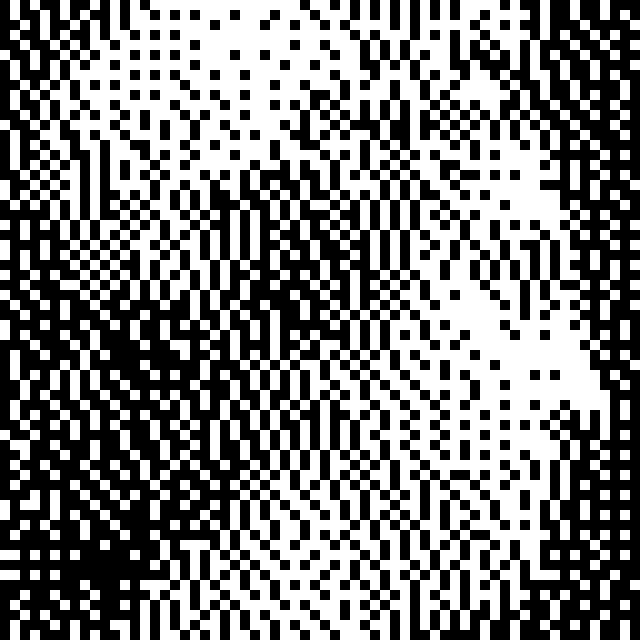
\includegraphics[width=\tilewidth,interpolate=false]{media/chp2/associative_memory/hopfield/07_00_orig_scaled_crushed.png}&%
		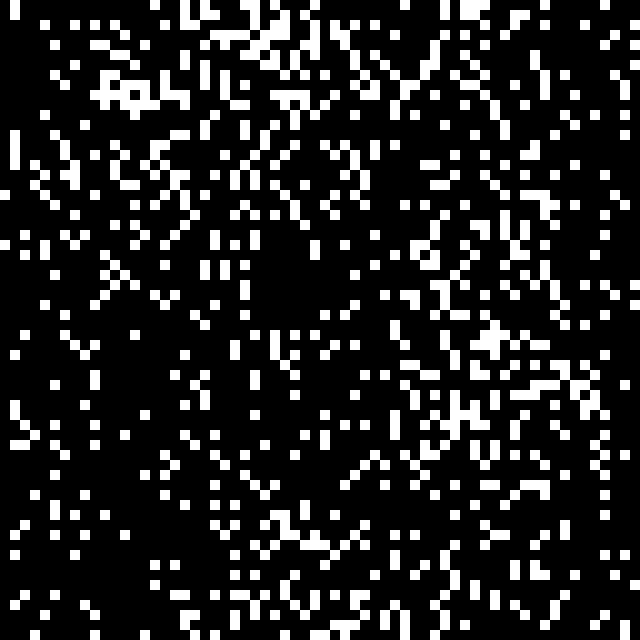
\includegraphics[width=\tilewidth,interpolate=false]{media/chp2/associative_memory/hopfield/07_01_noise_scaled_crushed.png}&%
		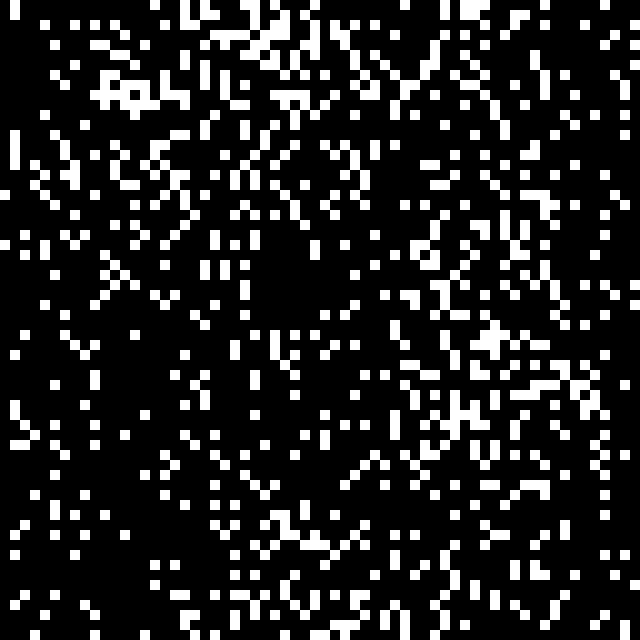
\includegraphics[width=\tilewidth,interpolate=false]{media/chp2/associative_memory/hopfield/07_02_activation_scaled_crushed.png}&%
		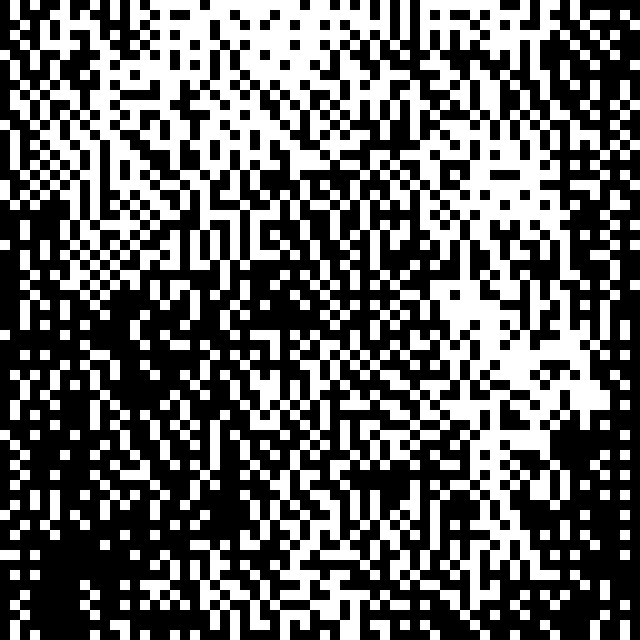
\includegraphics[width=\tilewidth,interpolate=false]{media/chp2/associative_memory/hopfield/07_03_activation_scaled_crushed.png}&%
		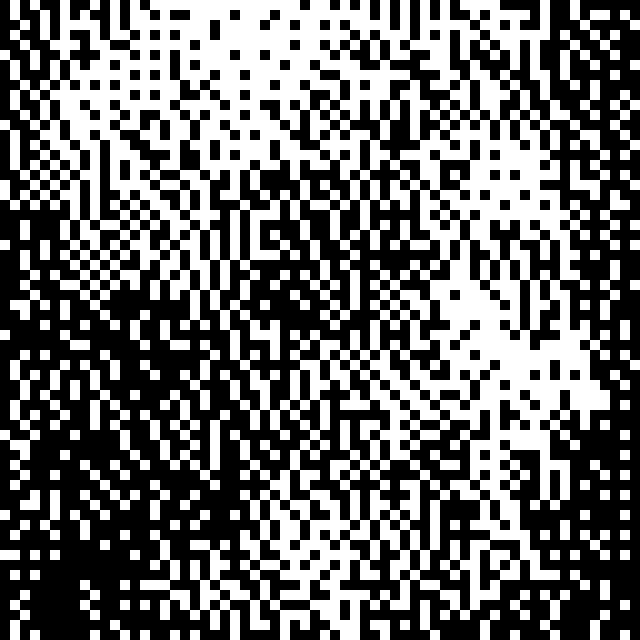
\includegraphics[width=\tilewidth,interpolate=false]{media/chp2/associative_memory/hopfield/07_04_activation_scaled_crushed.png}\\%
		(a) & (b) & (c) & (d) & (e)
	\end{tabular}
	\caption[Pattern completion in a Hopfield associative memory]{Example of pattern completion with a Hopfield associative memory. Column (a) shows $64 \times 64$ 1-bit images encoded as $4096$-dimensional column vectors $\vIn_k$. When presenting random $30\%$ of the original image as clue $\vIn$ to the memory (column (b)), it iteratively completes the patterns ((c)-(e)). Interference with four other stored images (not shown here) causes imperfect reproduction of the originals. The experiment is repeated with a \BiNAM in \cref{fig:binam_pattern_completion} (where all patterns are shown).}
	\label{fig:hopfield_pattern_completion}
\end{figure}

Along with artificial neural networks, technical implementations of associative memories have been researched since the middle of the last century, whereas the study of \enquote{associations} itself dates back to the ancient Greece philosopher Aristotle \cite{warren1916mental}. From our intuition it seems to be obvious that associations are an integral part of cognition: our brain constantly associates sensory input with internal states, such as feelings and memories, even if the two associated items are only connected remotely: consider the association of the smell of dry wood with the feeling of warmth at a fireplace. Of course, associations do not solely occur as a response to sensory input. Instead, they also play an important role in internal reasoning: often our mind follows a sequential chain of associations from one thought to the next until it suddenly \enquote{snaps} to the missing piece we have been searching for \cite{palm2013neural}.

Artificial associative memories aim at being high-level abstractions of the above concepts and merely touch the question on how associations actually work in human cognition. On the other hand, many associative memory models are implementable as neural networks and could be useful building blocks in artificial brain models. This section gives a quick conceptual overview of artificial associative memories and continues with a thorough description of the Willshaw model, its properties and implementation as a first-generation neural network.

\subsection{Artificial associative memory models}

Artificial associative memory models usually feature two phases: a \emph{training phase} in which input vectors $\vIn_k$ and the corresponding association $\vOut_k$ are presented to the model. In the \emph{recall phase} an arbitrary input vector $\vIn$ is fed into the system. In the optimal case the memory responds with the previously trained $\vOut_k$ corresponding to the trained input $\vIn_k$ to which $\vIn$ is closest according to a dissimilarity measure $\eth$
\begin{align}
	f(\vIn) = \vOut_k \quad \text{where} \quad k = \argmin_{k} \eth(\vIn_k, \vIn) \,.
	\label{eqn:associative_memory}
\end{align}
This concept resembles content addressed memory: data is not accessed by a physical address but by data itself, comparable to a hash map in computer science \cite{kohonen2012content}. Associative memories should also be clearly distinguished from function approximation in machine learning: the goal of associative memories is not to learn a generalised, continuous mapping between \vIn and \vOut, but to respond with one of the explicitly trained output vectors $\vOut_k$.

We distinguish two operational modes for associative memories: \emph{auto-association}, in which $\vIn_k = \vOut_k$ for all samples $k$, and \emph{hetero-association}, for which this equality is not presumed. As shown in \cref{fig:hopfield_pattern_completion}, auto-association can be interpreted as pattern-completion: given an altered (noisy) clue \vIn of a previously trained vector $\vIn_k$, the output of the memory converges towards a state resembling the original $\vIn_k$. Conversely, hetero-associations can be interpreted as semantic links between input $\vIn_k$ and output $\vOut_k$ \cite{palm2013neural}.

Hopfield networks, proposed in 1982, are one of the most famous associative memory models: they consist of a fully-connected network of McCulloch-Pitts cells (\cref{sec:mcculloch_pitts_neuron}) and operate on binary input and output vectors. During training, the synaptic weights $w_{ij}$ are set according to the \emph{Hebbian} learning rule \cite{hebb2005organization}. A connection between neuron $i$ and $j$ with $i \neq j$ is set to $w_{ij} = 1$ if $(\vIn_k)_i$ positively correlates with $(\vOut_k)_j$. Otherwise $w_{ij}$ is set to $w_{ij} = -1$
\begin{align}
	w_{ij} = \sign\left(\sum_{k} \big((\vIn_k)_i- \tfrac{1}2\big) \cdot \big( (\vOut_k)_j - \tfrac{1}2\big) \right) \,.
\end{align}
With this correlation based training scheme, the recurrent, fully-con\-nect\-ed network acts as a dynamical system with the trained output vector imprinted as attractors \cite{hopfield1982neural, hopfield2007hopfield}. Given an initial state $\vec x$, the network is likely to converge to the trained output $\vec y_k$ (\cref{fig:hopfield_pattern_completion}).

\subsection{Formal description of the Willshaw model}
\label{sec:binam_formal}

\marginnote{The output of the memory can of course be fed back to its input, which would result in a dynamical system and cause lots of fascinating behaviour. This is out of scope for this thesis.}
In contrast to Hopfield networks, the basic Willshaw associative memory model, or \acrfull{BiNAM}, does not describe a dynamical system. The model can be traced back to a paper by Steinbuch in 1961 \cite{steinbuch1961lernmatrix} and was independently described in 1969 by Willshaw \etal as a parallel, non-local and fault-tolerant associative network \cite{BiNAM1969}. It was further formalised and analysed by Palm \cite{palm1980associative}. Extensions of the model -- especially for spiking networks -- have, amongst others, been proposed by Knoblauch \cite{knoblauch2003synchronization, knoblauch2014structural}. Yet, as expounded in the introduction, we stick to the basic model.

Mathematically a \BiNAM can be defined as a binary storage matrix $\memMat \in \B^{\dimIn \times \dimOut}$, where $\B = \{0, 1\}$ is the base set of Boolean algebra, \dimIn is the dimensionality of the binary input vector $\vIn \in \B^{\dimIn}$ and \dimOut is the dimensionality of the output vector $\vOut \in \B^{\dimOut}$.

\paragraph{Training}
\begin{figure}
	\centering
	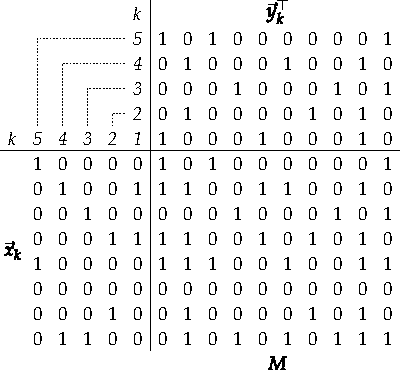
\includegraphics{media/chp2/binam_training.pdf}
	\caption[BiNAM training example]{Example of a $8 \times 10$ storage matrix \memMat after five samples $(\vIn_k, \vOut_k)$ with $\nOnesIn = 2$ ones in each input vector and $\nOnesOut = 3$ ones in each output vector have been trained according to \cref{eqn:binam_training}. The dotted lines connect input and output pairs.}
	\label{fig:binam_training}
\end{figure}
When training an association between an input $\vIn_k$ and output $\vOut_k$, the storage matrix \memMat is updated to a new \(\memMat'\)
\begin{align}
	\memMat' &= \memMat \vee \left( \vIn_k \cdot \transpose{\vOut_k} \right)\,,
	\label{eqn:binam_update_rule}
\end{align}
\marginnote{The condition \(\vIn_k = \vIn_\ell\) \(\Leftrightarrow k = \ell\) ensures unique input vectors: while it is possible for multiple \vIn to map to the same \vOut, it is prohibited for identical \vIn to map to multiple \vOut.}
where \enquote{$\vee$} is the element-wise \enquote{OR}-operation from standard Boolean algebra. If a set of \nSamples samples \((\vIn_k, \vOut_k)\)
\begin{align}
	\data = \{(\vIn_k, \vOut_k) \mid k \in \{1, \ldots, \nSamples\}\} \text{ with } \vIn_k = \vIn_\ell \Leftrightarrow k = \ell \,
	\label{eqn:binam_data}
\end{align}
is given in advance, a pre-calculated storage matrix \memMat can be obtained according to the following expression (\cref{fig:binam_training})
\begin{align}
	\memMat = \bigvee_{j = 1}^{\nSamples} \vIn_j \cdot \transpose{\vOut_j}\,.
	\label{eqn:binam_training}
\end{align}
\marginnote{Generation of data \data as used in the experiments conducted in this thesis is discussed in detail in \cref{sec:data_generation}.}
In this thesis we assume that such a pre-calculated storage matrix \memMat is already available --  we do not try to implement online training of the network. Additionally, and though not required for the operation of the \BiNAM, analysis of the memory is simplified significantly, if the number of bits set to \enquote{one} in both input and output vector is constant. We denote the number of \enquote{ones} in the input vectors \(\|\vIn_k\|_1\) as \(\nOnesIn\) and the number of \enquote{ones} in the output vectors \(\|\vOut_k\|_1\) as \(\nOnesOut\).

\paragraph{Recall}
\begin{figure}
	\centering
	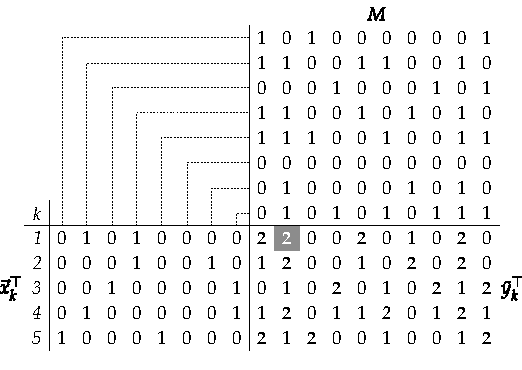
\includegraphics{media/chp2/binam_recall.pdf}
	\caption[BiNAM recall example]{Recalling the values associated to the \(\vIn_k\) previously trained in \cref{fig:binam_training}. The lower-right quadrant shows the intermediate results \(\transpose{\vOutI_k} = \transpose{\vIn_k} \cdot \memMat\) before applying the threshold function $\thresholdFunc_{\nOnesIn}$. Bold numbers correspond to those values that would be set to one in the final output, the grey backdrop signals a false-positive. The dotted lines connect rows in \memMat with their corresponding factors in the input data used when performing the vector-matrix multiplication.}
	\label{fig:binam_recall}
\end{figure}
In the recall phase, an arbitrary input vector \vIn is given. The output of the memory $\vOut$ can then be calculated as follows
\begin{align}
	\vOut &= \thresholdFunc_{\nOnesIn}(\vOutI) = 
		\thresholdFunc_{\nOnesIn}
			\left(\transpose{(\transpose{\vIn} \cdot \memMat)}\right)
		\quad \text{with} \quad
			\nOnesIn = \|\vIn\|_1 = \sum_{i = 0}^{\dimIn} (\vIn)_i = 
				\transpose{\vIn} \cdot \vIn\,,
	\label{eqn:binam_recall_rule}
\end{align}
\marginnote{Although the equation for \(\Theta_\theta\) looks fairly innocent, its realisation is the most crucial requirement for an operational spiking \BiNAM implementation.}
where $\thresholdFunc_{\threshold} : \N^{\dimIn} \longrightarrow \B^{\dimIn}$ is a step function with threshold \threshold, which maps the intermediate integer results of the matrix-vector multiplication \vOutI to binary values
\begin{align}
	(\thresholdFunc_{\threshold}(\vec z))_i
		&= \Heaviside\Big((\vec z)_i - \theta\Big) \,.
	\label{eqn:binam_threshold}
\end{align}
\cref{fig:binam_recall} shows the recall rule applied to the storage matrix \memMat previously trained in \cref{fig:binam_training}. As demonstrated, the recalled output of the \BiNAM is not perfect. A \emph{false positive} has been introduced (highlighted in grey): a one is present in component $j$ of the recalled output for \(\vIn_k\), although the trained \((\vOut_k)_j\) was set to zero.

\subsection{Choice of the threshold $\theta$}
\label{sec:binam_threshold}

Until now, the choice of \(\threshold = \nOnesIn\) in \cref{eqn:binam_recall_rule} has not been motivated. Consider a \BiNAM trained for a single sample \((\vIn_k, \vOut_k)\). The memory matrix is now set to $\memMat = \vIn_k \cdot \transpose{\vOut_k}$. Trying to recall \(\vOut_k\) by placing \(\vIn_k\) in \cref{eqn:binam_recall_rule} yields
\begin{align}
	\vOutI = \transpose{(\vIn_k \cdot \transpose{\vOut_k})} \cdot \vIn_k = \vOut_k \cdot (\transpose{\vIn_k} \cdot \vIn_k) = \vOut_k \cdot \nOnesIn \,.
\end{align}
Consequently, if a single sample is stored in the memory, the network returns an exact copy of the output vector \vOut scaled by \nOnesIn. Due to the additive superposition caused by the \enquote{$\vee$} in the training phase, newly trained samples can never lower the value of a single component $i$ in \vOutI, but only cause an increase towards the upper limit \nOnesIn
\begin{align}
%	\forall \memMat \in \B^{\dimIn \times \dimOut}, \vIn \in \B^{\dimIn}:
	(\vOutI)_i = (\transpose{\memMat} \cdot \vIn_k)_i \leq (\transpose{\memMat'} \cdot \vIn_k)_i \leq (\mathbb{1} \cdot \vIn_k)_i \leq \nOnesIn \,,
\end{align}
where $\mathbb{1}$ is the matrix of \enquote{ones} and
\begin{align}
	\memMat' &= \memMat \vee (\vIn \cdot \transpose{\vOut}) \text{ for any } \vIn \in \B^{\dimIn}, \vOut \in \B^{\dimOut}\,.
\end{align}
Given these considerations, adaptively setting the threshold \threshold to the maximum possible value $\nOnesIn = \|\vIn_k\|_1$, is the most sensible solution, as it minimises the chance of a false positive -- a bit in \vOut being set to one although it should be zero -- and yet prevents any \emph{false negatives}: all trained ones in the output are always present (see also \cref{sec:binam_failure_modes}).

\subsection{Storage capacity and sparsity}
\label{sec:binam_storage_capacity}

One of the defining properties of any memory is the amount of information that can be stored in the system. We refer to this measure as \emph{storage capacity}, or -- according to information theory -- \emph{information} or \emph{entropy}. Let us first consider the case of a conventional binary memory matrix \memMat of the size $\dimIn \times \dimOut$. Given a row index $k \in \{1, \ldots, \dimIn\}$ we can access any stored output vector $\vOut_k$. Each cell in $\vOut_k$ has two possible states, so the total number of possible $\vOut_k$ is $2^{\dimOut}$, and the number of possible matrices \memMat is $(2^{\dimOut})^{\dimIn}$. According to information theory, the number of bits \info needed to represent that many states is \cite{shannon2001mathematical}
\begin{align}
	\info = \lb((2^{\dimOut})^{\dimIn}) = \dimIn \cdot \lb(2^{\dimOut})= \dimIn \cdot \dimOut \,,
\end{align}
where $\lb$ is the binary logarithm. Given our constraint $\| \vOut_k \|_1 = \nOnesOut$, the amount of information is given as
\begin{align}
	\info = \lb\left(\binom{\dimOut}{\nOnesOut}^{\dimIn}\right) = \dimIn \cdot \lb \binom{\dimOut}{\nOnesOut}\,.
\end{align}

\begin{figure}[t]
	\centering
	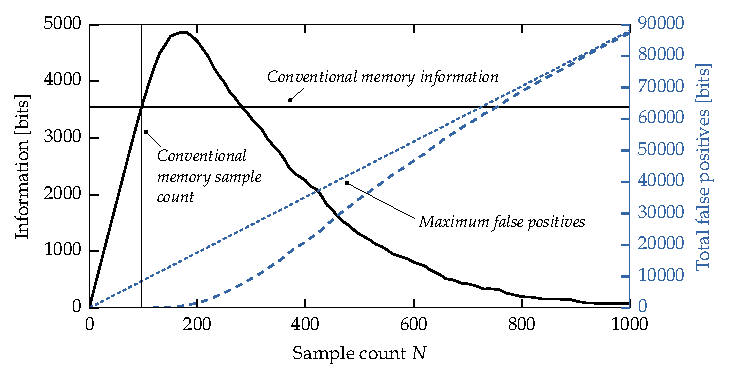
\includegraphics[trim=0.25cm 0.0cm 0.25cm 0.0cm,clip]{media/chp2/sketch_info.pdf}
	\caption[BiNAM information and false positive count over number of trained samples]{BiNAM information and false positive count over number of trained samples. Data size is $\dimIn = \dimOut = 96$, with $\nOnesIn = \nOnesOut = 8$. The optimal sample count is $\nSamples = 172$ with $\info = 4859$. For a conventional memory the same measures are $\nSamples = 96$ and $\info = 3\,547$.}
	\label{fig:sketch_info}
\end{figure}

\marginnote{For auto-associative storage measures see \cite{palm1980associative}.}
The same idea for the calculation of \info can be applied to associative memories in the hetero-association mode \cite{palm1980associative}. The only important difference between conventional and associative memories is the indexing scheme: output vectors $\vOut_k$ are not accessed by a row index $k$ but by a unique vector $\vIn_k$. In the case that all $\nSamples$ trained samples can be recalled perfectly, the storage capacity would be:
\begin{align}
	\info = \nSamples \cdot \lb \binom{\dimOut}{\nOnesOut}
\end{align}
\marginnote{The binomial coefficient $$\binom{\nOnesOut + \nFPk}{\nOnesOut}$$ expresses the number of ways in which the correct \nOnesOut ones can be distributed amongst the total number of ones in the output.}
However, as explained in \cref{sec:binam_threshold}, the probability of false positive bits in the output increases with the number of trained samples. Given the number of false positives \nFPk for a specific sample $k$, the possible number of states occupied by those wrong bits needs to be subtracted in the information calculation:
\begin{align}
	\info = \sum_{k = 1}^{\nSamples} \lb \binom{\dimOut}{\nOnesOut} - \lb \binom{\nOnesOut + \nFPk}{\nOnesOut}
	\label{eqn:binam_entropy}
\end{align}
If \nFNk false negatives are present in the output for sample $k$ (\cref{sec:binam_failure_modes}), an adapted equation must be used \cite{ruckert1991tolerance}:
\begin{align}
	\info = \sum_{k = 1}^{\nSamples}
			\lb\binom{\dimOut}{\nOnesOut}
		  - \lb\binom{\nFPk + \nOnesOut - \nFNk}{\nOnesOut - \nFNk}
		  - \lb\binom{\dimOut - \nFPk - \nOnesOut + \nFNk}{\nFNk}
	\label{eqn:binam_entropy_false_negatives}
\end{align}
As false positive and negative counts \nFPk and \nFNk are specific to the stored dataset and the actual $\vIn$ used for the recall operations, the storage capacity depends -- in contrast to conventional memory -- on memory content. \cref{fig:sketch_info} shows a simple experiment: a \BiNAM is trained with random data one sample at a time. After each sample has been trained, the stored information is calculated according to \cref{eqn:binam_entropy}, resulting in a characteristic information over sample count curve:
\marginnote{Achieving a higher storage capacity than conventional memories can be interpreted as intrinsic data compression in the \BiNAM. Given the information in the input $\vIn$, the $\vOut_k$ can be decompressed.}
the storage capacity \info quickly increases with the number of stored samples $\nSamples$, up to a certain maximum, and then converges to $\info = 0$ for large sample counts. In this particular example both the storage capacity \info and the number of stored samples significantly outperform the conventional memory.

However, this comes at a cost: for once, there is a chance of false positives in the output (the memory is not perfect) and the high storage capacity can only be reached if input and output vectors are \emph{sparse}: optimal performance is achieved if the number of ones $\nOnesIn, \nOnesOut$ are chosen logarithmic with respect to $\dimIn, \dimOut$. For non-sparse data the memory matrix \memMat converges to $\mathbb{1}$ too quickly, causing an increased false positive count \nFPk.

Note that the above restriction does not imply that the \BiNAM will not operate properly for non-sparse data -- the maximum storage capacity and the corresponding optimal sample count will just be smaller than that of conventional memories of the same size. An example of dense data storage in a \BiNAM is shown in \cref{fig:binam_pattern_completion}, which repeats the introductory pattern completion experiment from the beginning of this chapter with a \BiNAM instead of a Hopfield network. In contrast to the Hopfield network, the \BiNAM recalls all stored images perfectly in a single step.

Another conceptual property of the \BiNAM model is that it can be interpreted as a generalisation of a conventional memory. It gracefully reduces to such a memory if the $\vIn$  are appointed to \enquote{column selectors} which contain a single \enquote{one}, corresponding to $c = \|\vIn\| = 1$. Let, without any loss of generality, assume that the $\vIn_k$ are sorted such that $(\vIn_k)_k = 1$ and $\nSamples = \dimIn$
\begin{align}
	\memMat = \bigvee_{k = 1}^{\dimIn} \vIn_k \cdot \transpose{\vOut_k} = \transpose{(\vOut_1, \ldots \vOut_{\dimIn})} \Rightarrow \transpose{M} \cdot \vIn_k = \vOut_k \,.
\end{align}

\begin{figure}
	\footnotesize
	\centering
	\setlength{\tilewidth}{0.15\textwidth}
	\setlength{\tabcolsep}{2.75pt}
	\begin{tabular}{c c c c c c}%
		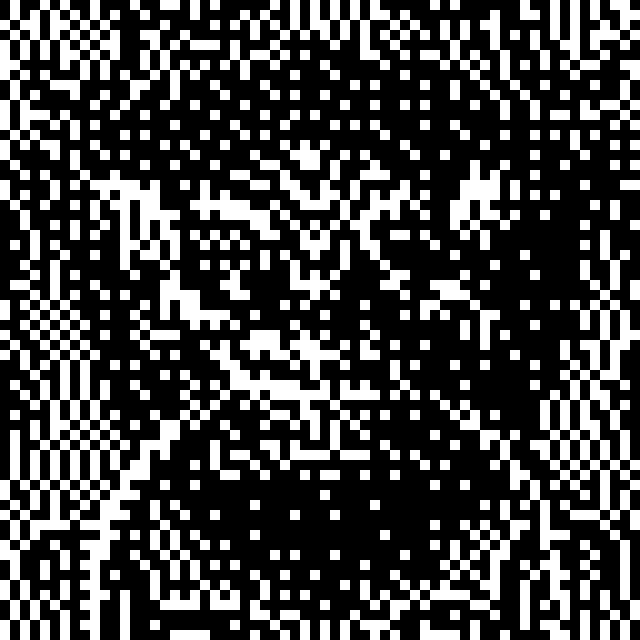
\includegraphics[width=\tilewidth,interpolate=false]{media/chp2/associative_memory/binam/00_00_orig_scaled_crushed.png}&%
		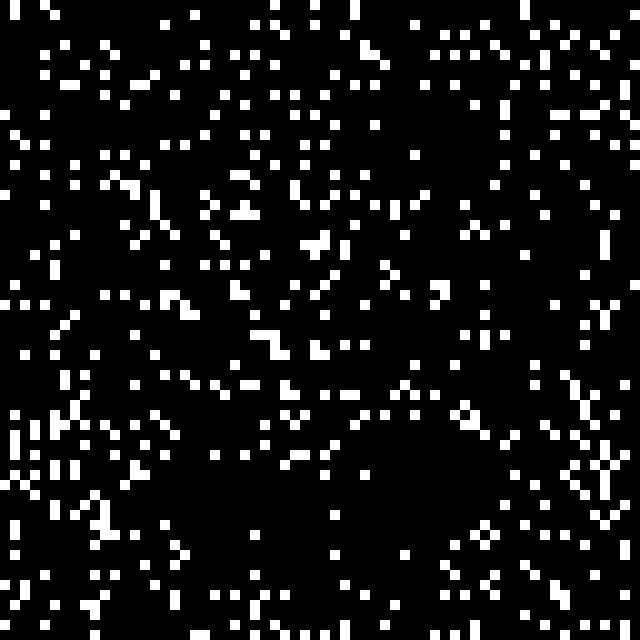
\includegraphics[width=\tilewidth,interpolate=false]{media/chp2/associative_memory/binam/00_01_noise_scaled_crushed.png}&%
		\includegraphics[width=\tilewidth,interpolate=false]{media/chp2/associative_memory/binam/00_02_out_scaled_crushed.png}&%
		\includegraphics[width=\tilewidth,interpolate=false]{media/chp2/associative_memory/binam/01_00_orig_scaled_crushed.png}&%
		\includegraphics[width=\tilewidth,interpolate=false]{media/chp2/associative_memory/binam/01_01_noise_scaled_crushed.png}&%
		\includegraphics[width=\tilewidth,interpolate=false]{media/chp2/associative_memory/binam/01_02_out_scaled_crushed.png}\\
		\includegraphics[width=\tilewidth,interpolate=false]{media/chp2/associative_memory/binam/02_00_orig_scaled_crushed.png}&%
		\includegraphics[width=\tilewidth,interpolate=false]{media/chp2/associative_memory/binam/02_01_noise_scaled_crushed.png}&%
		\includegraphics[width=\tilewidth,interpolate=false]{media/chp2/associative_memory/binam/02_02_out_scaled_crushed.png}&%
		\includegraphics[width=\tilewidth,interpolate=false]{media/chp2/associative_memory/binam/03_00_orig_scaled_crushed.png}&%
		\includegraphics[width=\tilewidth,interpolate=false]{media/chp2/associative_memory/binam/03_01_noise_scaled_crushed.png}&%
		\includegraphics[width=\tilewidth,interpolate=false]{media/chp2/associative_memory/binam/03_02_out_scaled_crushed.png}\\
		\includegraphics[width=\tilewidth,interpolate=false]{media/chp2/associative_memory/binam/04_00_orig_scaled_crushed.png}&%
		\includegraphics[width=\tilewidth,interpolate=false]{media/chp2/associative_memory/binam/04_01_noise_scaled_crushed.png}&%
		\includegraphics[width=\tilewidth,interpolate=false]{media/chp2/associative_memory/binam/04_02_out_scaled_crushed.png}&%
		\includegraphics[width=\tilewidth,interpolate=false]{media/chp2/associative_memory/binam/05_00_orig_scaled_crushed.png}&%
		\includegraphics[width=\tilewidth,interpolate=false]{media/chp2/associative_memory/binam/05_01_noise_scaled_crushed.png}&%
		\includegraphics[width=\tilewidth,interpolate=false]{media/chp2/associative_memory/binam/05_02_out_scaled_crushed.png}\\
		\includegraphics[width=\tilewidth,interpolate=false]{media/chp2/associative_memory/binam/06_00_orig_scaled_crushed.png}&%
		\includegraphics[width=\tilewidth,interpolate=false]{media/chp2/associative_memory/binam/06_01_noise_scaled_crushed.png}&%
		\includegraphics[width=\tilewidth,interpolate=false]{media/chp2/associative_memory/binam/06_02_out_scaled_crushed.png}&%
		\includegraphics[width=\tilewidth,interpolate=false]{media/chp2/associative_memory/binam/07_00_orig_scaled_crushed.png}&%
		\includegraphics[width=\tilewidth,interpolate=false]{media/chp2/associative_memory/binam/07_01_noise_scaled_crushed.png}&%
		\includegraphics[width=\tilewidth,interpolate=false]{media/chp2/associative_memory/binam/07_02_out_scaled_crushed.png}\\
		(a) & (b) & (c) & (a) & (b) & (c)
	\end{tabular}
	\caption[BiNAM pattern completion experiment]{BiNAM pattern completion experiment with non-sparse vectors: the binary $64 \times 64$ pixel images in the (a) columns are trained as 4096-dimensional vectors $\vIn_k$. Random $30\%$ of the \enquote{ones} in the original image are then presented as clue $\vIn$ to the memory (b). The recalled result is shown in (c). In this example all images are perfectly recalled by the \BiNAM.}
	\label{fig:binam_pattern_completion}
\end{figure}

\subsection{Neural network implementation}
\label{sec:binam_neural_network}

\begin{figure}
	\centering
	\includegraphics{media/chp2/binam_network.pdf}\\
	\caption[Neural network implementation of the BiNAM]{Neural network implementation of the BiNAM with McCulloch-Pitts cells. The $x_1, \ldots, x_{\dimIn}$ correspond to the components of an input vector $\vIn$, the $y_1, \ldots, y_{\dimOut}$ to the components of the output vector $\vOut$. Dots in the intersections between the neural input and the input components correspond to an excitatory synapse. These are inserted for all $i, j$ with $(\memMat)_{i, j} = 1$. The threshold \threshold is fixed in this implementation.}
	\label{fig:binam_network}
\end{figure}

Since its inception, the \BiNAM model has been proposed as \enquote{biologically plausible}: it can be easily implemented as a first- or second-generation artificial neural network, and the corresponding topology resembles certain structures in the brain \cite{BiNAM1969, palm1980associative}. Yet, before we consider the implementation, two notes should be taken into account: as already mentioned, our implementation is not capable of online training. Furthermore, it does not provide dynamic threshold adaptation. The impact of a fixed threshold \threshold is discussed in \cref{sec:binam_failure_modes}.

\marginnote{Of course, the model can also be implemented as firing-rate network: in this case, the threshold function $\thresholdFunc_{\threshold}$ has to be used as non-linearity $f$.}
Due to its binary nature, the \BiNAM model can be perfectly implemented with the McCulloch-Pitts neuron model (\cref{sec:mcculloch_pitts_neuron}). The network as shown in \cref{fig:binam_network} consists of a single layer of \dimOut neurons which receive the input signal \vIn, either as external input or from a sub-network. Each neuron corresponds to a single output component in \vOut. An excitatory synapse is added between input component $i$ and output neuron $j$ if, and only if, $(\memMat)_{i, j} = 1$. The threshold \threshold should be set to the average number of \enquote{ones} \nOnesIn in the trained input. Smaller or larger values than \nOnesIn may be required if noise is present in \vIn.

\subsection{Impact of noise}
\label{sec:binam_failure_modes}

% \info und I verwechslung

\begin{figure}[t]
	\centering
	\includegraphics{media/chp2/sketch_info_over_noise.pdf}\\
	\vspace*{0.25cm}
	\includegraphics{media/chp2/sketch_fps_over_noise.pdf}
	\includegraphics{media/chp2/sketch_fns_over_noise.pdf}
	\caption[Information measure and error count over noise]{Information measure and error count over noise parameters \pFn and \pFp. A \BiNAM of size $\dimIn = \dimOut = 96$ is trained with  $\nSamples = 172$ samples with $\nOnesIn = \nOnesOut = 8$ one-bits. The graphs show the total information and the averaged false positive and false negative counts for the recall of all trained samples. Addition and omission of bits are performed with probabilities \pFn and \pFp. The behaviour between fixed and adaptive threshold \threshold is compared. In the fixed threshold case $\threshold = \dimIn = 8$.}
	\label{fig:sketch_info_over_noise}
\end{figure}

Aside from the pattern completion example in \cref{fig:binam_pattern_completion}, perfect conditions were assumed up to this point: the input vectors $\vIn_k$ presented to the network in the recall phase are the same as in the input data \data actually learned in the training phase. As noted above, even in this scenario there is the possibility of \emph{false positives}. This failure mode results from the storage matrix continuously getting saturated during training. If the \enquote{ones} in the training samples are uniformly distributed, the memory matrix \memMat asymptotically approaches the \enquote{ones} matrix $\mathbb{1}$ (\cref{sec:binam_random_data_behaviour}).

There are two ways in which we can corrupt the originally trained input vectors $\vIn_k$: by addition (additional bits are set to one) and by omission (bits originally set to one are set to zero). In the case of additive noise, the input vector \vIn can be modelled as
\begin{align}
	(\vIn)_i = (\vIn_k)_i \vee \eta \text{ with } \probability{(\eta = 0)} = 1 - \pFp \text{ and } \probability{(\eta = 1)} = \pFp \,,
\end{align}
where \pFp is the probability of an arbitrary input vector component being set to one. In the omission (multiplicative) case, the input vector \vIn can be modelled as
\begin{align}
	(\vIn)_i = (\vIn_k)_i \wedge \eta \text{ with } \probability{(\eta = 0)} = \pFn \text{ and } \probability{(\eta = 1)} = 1 - \pFn \,,
\end{align}
where \pFn is the probability of an arbitrary input vector component being set to zero. 

\cref{fig:sketch_info_over_noise} shows the impact of the two kinds of noise on storage capacity, \emph{false positive} and \emph{false negative} counts. It furthermore distinguishes between an adaptive threshold $\threshold = \|\vIn\|_1$ and a fixed threshold $\threshold$. For multiplicative noise and adaptive threshold, the information \info decreases almost linearly with \pFn. Counter-intuitively, the false-positive count increases the more bits are omitted in the input. This is caused by the missing input bits lowering the threshold \threshold. For a fixed threshold, the false-positive count converges to zero with increasing \pFn, accompanied with an increase in the false-negative count. Correspondingly, the information measure drops to zero.

Additive noise has a much stronger negative impact on the storage capacity as its multiplicative counterpart. First of all, this is caused by \pFp and \pFn not being directly comparable: due to sparsity, the probability of adding an additional \enquote{one} to the input is higher than setting an actual \enquote{one} to zero in the multiplicative case. If no adaptive threshold is used, the false positive count quickly rises towards the maximum. With adaptive threshold, the addition of input bits causes false negatives as the increased threshold masks the correct \enquote{ones}. In both cases the information measure \info drops to zero.

To summarise the possible \BiNAM failure modes: false positives can always be produced, even without noise. False negatives occur if input bits are missing and the threshold is not adapted (as in our neural network implementation, \cref{sec:binam_neural_network}), and if \threshold is increased above \nOnesIn due to additional input bits.


\section{Summary and outlook}

This chapter provided a scenic overview of various fields of research. We discussed neural network models, both from the view of neurobiology and neuroinformatics, and their implementation in neuromorphic hardware. Furthermore, we have thoroughly investigated the Willshaw associative memory and provided an implementation in the form of an artificial, first-generation neural network.

In \cref{chp:spinam}, we combine these building-blocks: we extend our \BiNAM implementation towards spiking neural networks and provide the workflow for design space exploration. In \cref{chp:neuron_evaluation}, we dive back into the details of the \LIF and \AdEx spiking neural network models to find proper values for the neuron parameters listed in \cref{tbl:adex_parameters}. Finally, in \cref{chp:experiments}, we pioneer into the realm of neuromorphic hardware and boldly execute the model on platforms, on which no associative memory has run before.

\chapter{Spiking Associative Memory Architecture and Testing}
\label{chp:spinam}

\marginnote{The spiking implementation of the Willshaw associative memory is no longer truly \enquote{binary} (regarding weights and timings). Therefore the name ``\BiNAM'' might be a little misleading when referring to spiking neural networks; however, the same name is used in this thesis for the sake of consistency.}
The previous chapter introduced the Willshaw associative memory model (\BiNAM) and the notion of spiking neural networks. In this chapter we merge those two concepts: \cref{sec:neural_network_topology} describes the transition of the \BiNAM architecture from a firing-rate coded to a spiking neural network. Furthermore, to account for the spiking network time dynamics, we specify the general testing procedure, how input and output data are encoded as a sequence of spikes, and how noise in the input data is parametrised in a spiking environment. \cref{sec:memory_evaluation_measures} introduces multiple measures for the quantification of the network performance, while \cref{sec:data_generation} focuses on the generation of datasets that can be used for network evaluation.

\section{Neural network topology and data encoding}
\label{sec:neural_network_topology}

\begin{figure}
	\centering
	\subbottom[Single neuron]{
		\includegraphics{media/chp3/spinam_topology_a.pdf}
		\label{fig:spinam_topology_a}
	}
	\subbottom[Population of $\populationSize = 2$]{
		\includegraphics{media/chp3/spinam_topology_b.pdf}
		\label{fig:spinam_topology_b}
	}
	\caption[Comparison between a single neuron BiNAM implementation and its population counterpart]{Two possible implementations of a $j$-th \BiNAM column as spiking neural network: in (a) the network is implemented as a one-to-one translation of the firing-rate neural network topology. In (b) each neuron is replaced by a population of \populationSize neurons ($\populationSize = 2$ in this example); memory input and output components are represented by \populationSize independent signals, $y^1_j, \ldots, y^{\populationSize}_j$.}
	\label{fig:spinam_topology}
\end{figure}

The most trivial way of implementing the Willshaw associative memory model as spiking neural network is to directly employ the firing-rate network topology introduced in \cref{sec:binam_neural_network}: if an entry in the trained storage matrix \((\memMat)_{ij}\) is set to \enquote{one}, a synaptic connection between the neuron $j$ in the output layer and input $i$ in the input layer is established. This basic topology is sketched in \cref{fig:spinam_topology_a}. Another possible topology is shown in \cref{fig:spinam_topology_b}: instead of single neurons, a population of neurons represents each output component, with input and output being transmitted via connection bundles. This topology is presented in detail in \cref{sec:neuron_populations}.

Difficulties in building a spiking neural network arise from the time dynamics: we need to think about how input and output data are represented as a sequence of spikes in the time domain. We consider this problem in more detail in \cref{sec:input_output_time_window,sec:input_data_parametrisation}.

Furthermore, synapse weights are no longer dimensionless scalars which can be trivially mapped to the ones and zeros in \memMat. Instead, each synapse possesses a conductivity measured in siemens. While zeros in \memMat can be mapped to a synapse with zero conductivity (corresponding to no synapse at all), the conductivity $w$ representing a \enquote{one} in \memMat needs to be carefully selected.

\marginnote{Even if we had to implement a \BiNAM as a firing-rate neural network with fixed non-linearity, the threshold could be easily implemented with a sub-network trained for this task via back-propagation. Such a simple training of spiking neural networks is not possible.}
Another problem concerns the threshold in the \BiNAM recall rule from \cref{eqn:binam_recall_rule}: whereas the McCulloch-Pitts neuron model provided a perfect threshold function, single neurons in a spiking neural network do not offer such a well-behaved transfer function. The transfer function is specified as dynamical system which can only be affected by neuron parameter adaptation. This selection of neuron parameters is non-trivial.

In \cref{sec:required_neuron_behaviour}, we discuss the neuron behaviour required for a functioning \BiNAM, given the data representation and the general network topology from the previous sections. We could then try to tune the neuron parameters and synapse weight \(w\) with respect to these rules. This endeavour is the topic of the next chapter \ref{chp:neuron_evaluation}.

\subsection{Input-/output spike sequences}
\label{sec:input_output_time_window}

\begin{figure}
	\centering
	\includegraphics{media/chp3/spinam_nomenclature.pdf}
	\caption[Spiking BiNAM implementation and spike train nomenclature]{Test environment for the spiking implementation of a $5 \times 4$ \BiNAM. The bold marks represent input/output spikes with examples of the spike train nomenclature in \cref{eqn:spike_train_nomenclature}.}
	\label{fig:spinam_nomenclature}
\end{figure}

\begin{figure}
	\centering
	\includegraphics{media/chp3/classical_spiking_comparison.pdf}
	\caption[Comparison between a classical and spiking neural network]{Conceptual comparison between the operation of a classical and spiking neural network: the classical neural network maps between discrete input and output vectors $\vIn_k \mapsto \vOut_k$. Such a mapping has to be artificially created on the input/output of a spiking network by assigning output spikes to the closest past input spike. Dotted vertical lines indicate the first spike belonging to a new sample.}
	\label{fig:classical_spiking_comparison}
\end{figure}

Classical feed-forward firing-rate coded neural networks do not possess time-dynamics: they merely describe a mathematical function $f$ which maps vectorial input $\vIn_k$ onto output $\vOut_k$. The network does not possess any hidden state that may be influenced by previous computations, that is, there are no side-effects. Individual operations -- for example a recall in an associative memory -- are strictly separated from each other. When dealing with time-series of data, an evaluation of $f$ can usually be executed within a single simulation time step.

\marginnote{Of course, separation between individual samples could be forced by repeatedly resetting the simulation. Yet, this may neither be practical (the network state may be important), nor possible (neuromorphic hardware).}
Spiking neural networks do not share these properties: there exists no direct mapping between input and output; both are represented by a stream of continuous spike times, with each spike influencing the state of the involved neurons over time. For closed-loop operation this asynchronicity is one of the defining properties of a spiking neural network. For the sample based performance evaluation of our memory, we need to group input and output spikes that belong to the same sample $(\vIn_k, \vOut_k)$. As network simulations and especially neuromorphic hardware systems do not (or at least not consistently across platforms) allow to dynamically inject spikes during runtime, the entire input spike stream has to be assembled ahead of time and the network output has to be matched in a post-processing step.

To describe our solution to this problem, we first need to specify the spiking \BiNAM test environment (\cref{fig:spinam_nomenclature}): an input layer, a group of \dimIn programmable spike sources, emulates external input to the network. Each source represents a single component $i$ in \(\vIn_k\) and produces a pre-programmed spike train \tInI, which can be described as an ordered sequence of spike times \(t^{\mathrm{in}}_{i,\ell}\)
\begin{align}
	t^{\mathrm{in}}_i &= (
		t^{\mathrm{in}}_{i, 1},
		t^{\mathrm{in}}_{i, 2},
		\ldots) \quad
		    \text{ with } \quad t^{\mathrm{in}}_{i, \ell} \leq t^{\mathrm{in}}_{i, \ell'} \Leftrightarrow \ell \leq \ell' \,.
	\label{eqn:spike_train_nomenclature}
\end{align}

During test execution output spikes \tOutJ are recorded from the output layer, which consists of \dimOut neurons performing the actual thresholding operation. Analogously to the input spike times, \(t^{\mathrm{out}}_{j,\ell}\) denotes the $\ell$-th spike for the $j$-th output component \(\vOut_k\).

In order to assemble \tInI, input samples $\vIn_k$ are converted into their spike time representation (discussed in \cref{sec:input_data_parametrisation}). Let $k^{\mathrm{in}}_{i, \ell}$ denote the sample index each spike $t^{\mathrm{in}}_{i, \ell}$ belongs to. As depicted in \cref{fig:classical_spiking_comparison}, a simple approach for assigning output spikes \(t^{\mathrm{out}}_{j,\ell}\) to the sample $k$ they are most likely associated to, is by selecting $k^{\mathrm{out}}_{j, \ell}$ as the sample index of the latest input spike issued before \(t^{\mathrm{out}}_{j,\ell}\)
\begin{align}
	k^{\mathrm{out}}_{j, \ell} &= k^{\mathrm{in}}_{i, \ell'} \quad \text{with} \quad i, \ell' = \argmin_{i, \ell'}\{t^{\mathrm{out}}_{j,\ell} - t^{\mathrm{in}}_{i,\ell'} \mid t^{\mathrm{out}}_{j,\ell} - t^{\mathrm{in}}_{i,\ell'} > 0 \} \,.
	\label{eqn:spike_train_matching}
\end{align}
In case the network utilises the already mentioned \enquote{neuron population}-topology from \cref{sec:neuron_populations}, there may be multiple neurons for a single input/output component. For sake of simplicity regarding the above equations, we assume that spikes from multiple neurons for the same component $j$ are fused into a single, virtual spike train.

\begin{figure}
	\centering
	\vspace*{0.575cm}
	\includegraphics{media/chp3/spike_train_shift.pdf}\\
	\vspace*{0.575cm}
	\caption[Example of input sample pipelining]{Example of input sample pipelining: virtually shifting the output spike times back by $\zeta$ allows higher input sample rate $T'$ while preserving the spike-sample matching (colour coded). Note how the higher sample rate affects the output.}
	\label{fig:spike_train_shift}
\end{figure}
Propagation of a signal through the network is usually not instantaneous. Thus, it can happen that an output spike is mapped to an input spike that already belongs to a later sample. If the minimum delay $\zeta$ between the first input and output spike of a sample is known, the output spike train can be virtually shifted back by $\zeta$ for the calculation of $k^{\mathrm{out}}_{j, \ell}$ according to \cref{eqn:spike_train_matching}
\begin{align}
	i, \ell' = \argmin_{i, \ell'}\{t^{\mathrm{out}}_{j,\ell} - \zeta - t^{\mathrm{in}}_{i,\ell'} \mid t^{\mathrm{out}}_{j,\ell} - \zeta - t^{\mathrm{in}}_{i,\ell'} \geq 0 \} \,.
\end{align}
As shown in \cref{fig:spike_train_shift}, this potentially allows to pack input samples tighter without risking misclassification due to output spikes already being matched with the next sample. The technique can be used to implement pipelining of the memory recall operations. Note however, that due to the statefulness of the network, a higher input sample rate will affect the output.

\subsection{Data encoding and input noise parametrisation}
\label{sec:input_data_parametrisation}

We now need to decide on how to encode a single one-bit as a time sequence of spikes. In case the memory receives input from other networks -- or artificial test data -- which follows this 
specification, we expect our network to respond with another valid output spike pattern in this encoding.
A straight-forward approach is to represent each one-bit in $(\vIn_k$, $\vOut_k)$ as a single spike. So in order to recall a vector for input $\vIn_k$ from the memory, we send a spike to all inputs $i$ with $(\vIn_k)_i = 1$ at a certain time $t = \timeWindow \cdot k$, where the constant \timeWindow is the time between two input samples. The output component $(\vOut_k)_j$ is set to one, if an output spike with assigned sample index \(k^{\mathrm{out}}_{j, \ell} = k\) exists.

We expand this data generation scheme in two ways: by representing ones with potentially more than a single spike, resulting in \emph{bursts}, and by modelling time noise, \emph{jitter}, in the input.

\paragraph{Bursts}
Neurons in the cortex often operate in a \emph{phasic bursting} mode in which action potentials occur in groups of multiple spikes (\cref{fig:isi_decay}), henceforth called \emph{bursts} \cite{connors1990intrinsic}. From a theoretical point of view signalling events using bursts has at least two advantages: they increase the robustness in case of noise -- for example if a single spike out of multiple is lost (as it might happen in both biological and neuromorphic hardware systems), the information about the corresponding event is not irrecoverably destroyed, and if false-positive single spikes are received by a neuron, these can be filtered out \cite{lisman1997bursts}. Secondly, bursts allow to encode analogue values, either by variation of the spike count or the spike frequency within the burst.

To interface with \enquote{bursting} networks our associative memory implementation should support arbitrary integral burst sizes \burstSizeIn and \(\burstSizeOut \geq 1\) chosen at design time. The network has to accept bursts of size \burstSizeIn at the input, but it must also produce \burstSizeOut spikes for each one-bit in the output.

\marginfig{Sketch of a burst with increasing interspike interval}{
\includegraphics{media/chp3/isi_decay.pdf}
}{Sketch of a neuron membrane potential over time showing spikes from a burst with decaying interspike interval $\isi$.}{\label{fig:isi_decay}}
When generating artificial bursts as test input, we parametrise these with an equidistant \ISI \(\isi\). Note that this is only a coarse model of actual data that might be encountered in a large network, where the interspike interval may be inconsistent: for example in the \AdEx model, the interspike interval is likely to increase over time (\cref{sec:adex} and \cref{fig:isi_decay}). For small \burstSizeIn this effect should be relatively subtle and selecting a constant \isi as the average interspike interval is a reasonable approximation.

On the output side, bursts imply fractional output values whenever a number of spikes that differs from the expected burst size \burstSizeOut is generated. We redefine the value of the output component \((\vOut_k)_j\) as the quotient of the number of actual number of spikes encountered in the output time window, divided by the expected burst size \burstSizeOut
\begin{align}
	(\vOut_k)_j = \frac{| \{k^{\mathrm{out}}_{j, \ell} = k\} |}{\burstSizeOut}
	\label{eqn:spiking_output_values} \,.
\end{align}
To cope with arbitrary \enquote{fractional bit values} in the theoretical \BiNAM storage capacity measure, we introduce an adapted version of the corresponding storage capacity equation (\ref{eqn:binam_entropy_false_negatives}) in \cref{sec:eval_storage_capacity}.

\paragraph{False negative and positive input spikes}
In \cref{sec:binam_failure_modes}, we discussed missing and additional one-bits in the input vectors, where the corresponding events were modelled with probabilities \pFn and \pFp. The representation of one-bits as a series of $\burstSizeIn$ spikes allows to insert and remove individual spikes instead of bits. Thus \pFn is used to describe the probability of skipping a single spike from a burst representing a \enquote{one}, while \pFp describes the probability to issue a single spike from a virtual burst when encoding a \enquote{zero}.

For large burst sizes \burstSizeIn the probability of an entire input burst being removed or added is relatively small (\pFn and \pFp to the power of \burstSizeIn). This is intentional, as the effects of entire bursts being removed and added can be well studied within the theoretical \BiNAM framework (\cref{sec:binam_failure_modes}). For the spiking implementation we want to focus on noise concerning individual spikes instead.

\paragraph{Jitter}
Due to the involved dynamic systems, it is implausible for spiking neural networks to generate perfect timings. In order to emulate these imperfections, we add small time offsets, \emph{jitter}, to the spikes.
\marginnote{Data show that cortical neurons can reproduce spike patters with millisecond precision under laboratory conditions \cite{mainen1995reliability}.}
In our model we sample a random offset from a Gaussian distribution with standard deviation \jitter for each spike time $t^{\mathrm{in}}_{i, \ell}$. Additionally, we shift the entire burst by \jitterMeanOffs in order to model synaptic or spatial delays. Again, \jitterMeanOffs is sampled from a Gaussian distribution with standard deviation \jitterOffs.

\begin{figure}
	\centering
	\includegraphics{media/chp3/burst_example.pdf}
	\caption[Parametrisation of an example input spike burst with jitter]{Parametrisation of an example input spike burst of size $\burstSizeIn = 5$ with jitter as described in \cref{eqn:input_spike_burst}. Bold marks correspond to the generated spike times $t_1, \ldots, t_5$. The bell-shaped functions visualise the Gaussian distributions from which the time offset \jitterMeanOffs (dashed) and the individual spike times $t_i$ (blue) are sampled.}
	\label{fig:burst_example}
\end{figure}
\marginnote{As time offsets are drawn from a Gaussian distribution, it might hold $t_{\ell - 1} \geq t_{\ell}$. To allow for computationally efficient processing, a generated sequence of spike times should be sorted in a software implementation.}
An input burst for the $k$-th sample can thus be described as a sequence of \burstSizeIn random variables \((t_1, \ldots, t_{\burstSizeIn})\)
\begin{align}
	t_\ell &\sim \mathcal{N}\Big(k \cdot \timeWindow + \jitterMeanOffs + \isi \cdot (\ell - 1), \jitter\Big) \text{ with } \jitterMeanOffs \sim \mathcal{N}(0, \jitterOffs) \,.
	\label{eqn:input_spike_burst}
\end{align}
Note that the offset \jitterMeanOffs is not an independent random variable for each $t_i$. Instead, it is sampled once for all spike times $t_i$ within the burst.

\begin{table}
	\centering
	\small
	\begin{tabular}{r p{10.1cm}}
		\toprule
		\multicolumn{2}{c}{\spacedlowsmallcaps{Network and input/output parametrisation}} \\
		\midrule
		\multicolumn{2}{c}{\slshape Network and data parameters} \\
		\midrule
		\dimIn, \dimOut & Number of input and output components. \\[0.5em]
		\nOnesIn, \nOnesOut & Number of \enquote{ones} in each input/output sample.\\[0.5em]
		\nSamples & Number of input samples.\\[0.5em]
		\populationSize & Number of neurons representing each output component.\\
		\midrule
		\multicolumn{2}{c}{\slshape Output data parameters} \\
		\midrule
		\burstSizeOut & Output burst size: number of spikes produced by a single neuron in an output burst which represents a \enquote{one}. For neuron populations ($\populationSize > 1$), each individual neuron is expected to produce this number of spikes.\\
		\midrule
		\multicolumn{2}{c}{\slshape Input data parameters} \\
		\midrule
		\burstSizeIn & Input burst size: number of spikes sent in an input burst to a single neuron. For populations, each individual neuron receives $\populationSize$ input bursts of this size.\\[0.5em]
		\timeWindow & Average time between input samples.\\[0.5em]
		\isi & Equidistant interspike interval between input spikes in a burst.\\
		\midrule
		\multicolumn{2}{c}{\slshape Input data noise parameters} \\
		\midrule
		\jitter & Standard deviation of the Gaussian distribution the input spikes are selected from.\\[0.5em]
		\jitterOffs & Standard deviation of the random variable from which the spike burst offset is chosen. Models synaptic or spatial signal delays.\\[0.5em]
		\pFn & Probability of skipping a spike (false-negative) in an input burst when generating a \enquote{one}.\\[0.5em]
		\pFp & Probability of adding a superfluous (false-positive) spike from a virtual input burst when generating a \enquote{zero}.\\
		\bottomrule
	\end{tabular}
	\caption[Network and input/output parametrisation]{Summary of network,  input/output and input noise parameters.}
	\label{tbl:input_data_parametrisation}
\end{table}
\begin{algorithm}
	\small
	\begin{shaded}
		\begin{algorithmic}[1]
			\newcommand{\To}{\textbf{to}\xspace}
			\newcommand{\Init}{\State\textbf{init}\xspace}
			\Function{GenerateInput}{$M, \nSamples, \populationSize, \burstSizeIn, \timeWindow, \isi, \jitter, \jitterOffs, \pFn, \pFp$}
				\Init $t^{\mathrm{in}}_{m, k} \gets () \; \forall \; m \in \{1, \ldots, M\}, k \in \{1, \ldots, \populationSize\}$
				\For{$n \gets 1$ \To $\nSamples$} \Comment{Iterate over all samples}
					\For{$m \gets 1$ \To $\dimIn$} \Comment{Iterate over all input components}
						\If{$(\vIn_n)_m = 1$} \Comment{Set spike omission probability $p$}
							\State $p \gets \pFn$
						\Else
							\State $p \gets 1 - \pFp$
						\EndIf
						\For{$k \gets 1$ \To $\populationSize$} \Comment{Iterate over all neurons in the population}
							\State $t^\mathrm{offs} \gets $ \Call{Normal}{$n \cdot \timeWindow$, \jitterOffs} \Comment{Select burst time offset}
							\For{$\ell \gets 1$ \To $\burstSizeIn$} \Comment{Iterate over all spikes}
								\If{\Call{RandomSelect}{$[0, 1)$}$ \geq p$}
									\State $t^{\mathrm{in}}_{m, k} \gets t^{\mathrm{in}}_{m, k} \Arrowvert $ \Call{Normal}{$t^\mathrm{offs} + (\ell - 1) \cdot \isi$, \jitter}
									\State $k^{\mathrm{in}}_{m, k} \gets k^{\mathrm{in}}_{m, k} \Arrowvert n$
								\EndIf
							\EndFor
						\EndFor
					\EndFor
				\EndFor
				\State $k^{\mathrm{in}}_{m, k} \gets$ \Call{SortByKey}{$k^{\mathrm{in}}_{m, k}, t^{\mathrm{in}}_{m, k}$} $\forall m, k$ \Comment{Sort indices by spike times}
				\State $t^{\mathrm{in}}_{m, k} \gets$ \Call{Sort}{$t^{\mathrm{in}}_{m, k}$} $\forall m, k$ \Comment{Sort spike times}
				\State \Return $\tIn, \kIn$
			\EndFunction
		\end{algorithmic}
	\end{shaded}
	\caption[Input burst generation algorithm]{Input spike train generation algorithm. Generates the input spike trains \tIn and indices \kIn for all neurons according to the data parameters in \cref{tbl:input_data_parametrisation}. For a more consistent notation inside the algorithm, the input dimensionality is denoted as $M$ instead of \dimIn.}
	\label{alg:input_data_generation}
\end{algorithm}
A diagram showing the involved variables is given in \cref{fig:burst_example}, along with an overview of all discussed parameters in \cref{tbl:input_data_parametrisation} and an algorithm for the generation of an input spike sequence for a single input bit $(\vIn_k)_i$ in \cref{alg:input_data_generation}.

\subsection{Neuron populations}
\label{sec:neuron_populations}

\marginnote{The Poisson-distribution
	\[P_\lambda(k) = \frac{\lambda^k}{k!} e^{-\lambda}\]
	describes the probability of an event to occur $k$-times in a certain time interval, given its average rate is $\lambda$.}
Findings regarding neural codes in the cortex suggest that neuron spike patterns can be modelled by a Poisson process \cite{softky1993highly}. This implies that single spike times convey little information -- the instantaneous activity of neural circuitry can only be estimated when pooling responses from multiple neurons. It thus seems likely that neural networks are built redundantly, and information is encoded in the correlation of spike patterns originating from a \emph{population} of neurons \cite{shadlen1994noise}.

With respect to our scenario, the following changes to the network topology take these considerations into account: we replace each neuron $u_j$ with a population of \populationSize neurons $u_j^1, \ldots, u_j^{\populationSize}$, in which each fires a small number of \burstSizeOut spikes per one-bit in the output component $(\vOut)_j$. These neurons receive the same input and all output signals $y_j^1, \ldots, y_j^{\populationSize}$ are fed in parallel to the next input. The signals are treated as a single output $y_j$ for evaluation purposes. As the total number of output spikes for an output component is now given as $\populationSize \cdot \burstSizeOut$, a relatively small burst size can be used (possibly $\burstSizeOut = 1$). Analogously to \cref{eqn:spiking_output_values}, the value of the output component $j$ can be calculated as
\begin{align}
	(\vOut_k)_j = \frac{| \{k^{\mathrm{out}}_{j, \ell} = k\} |}{\populationSize \cdot \burstSizeOut} \,.
	\label{eqn:spiking_output_values_population}
\end{align}

Besides biological plausibility this architecture has two other potential advantages: tuning the neuron parameters in such a way that they produce a small number of spikes might turn out to be easier to accomplish than selecting neuron parameters which cause the neuron to reliably produce an exact large number of output spikes. Furthermore, the redundancy introduced by the neuron populations allows single neurons to fail without severely impacting the network performance.

On the downside, the number of required neurons scales linearly with \populationSize, the number of required synapses scales quadratically with \populationSize, inevitably increasing both size and energy consumption of the network. An example of the topology for $\populationSize = 2$ is sketched in \vref{fig:spinam_topology_b}.

\subsection{Required neuron behaviour}
\label{sec:required_neuron_behaviour}

We have discussed two possible \BiNAM spiking neural network topologies. We now need to specify the neuron behaviour required for the operation of the network. Basically, there are two conditions each neuron in the network must fulfil: the \emph{threshold condition} and the \emph{reset condition}.

\paragraph{Threshold condition}
As specified in the \BiNAM recall rule in \cref{eqn:binam_recall_rule}, the neuron needs to fulfil a thresholding behaviour: let $n_{\mathrm{in}}$ denote the number of input spikes within an input time frame of approximately $\isi \cdot \burstSizeIn$. The number of output spikes the neuron should produce in response to this input is then given as
\begin{align}
	n_{\mathrm{out}}(n_{\mathrm{in}}) &= \begin{cases}
							\burstSizeOut
								& \text{if } n_{\mathrm{in}} \geq \threshOne = \nOnesIn \cdot \burstSizeIn \cdot \populationSize \\
							0
								& \text{if } n_{\mathrm{in}} \leq \threshZero = (\nOnesIn - 1) \cdot \burstSizeIn \cdot \populationSize
	                    \end{cases} \;\;\;\;.
	\label{eqn:threshold_condition}
\end{align}

For input spike counts in the interval $(\threshZero, \threshOne)$, the neuron behaviour is deliberately left undefined, as these values should not occur under perfect conditions and a sharp threshold such as $\threshZero = \threshOne - 1$ would be very demanding to realise.

It should also be stressed, that the neuron parameters for the realisation of the threshold behaviour can only be chosen for a constant time frame $\isi \cdot \burstSizeIn$. At some point, if input spikes arrive in a shorter or longer period of time, more or fewer output spikes will be certainly generated due to the fixed neuron time dynamics. However, we can try to maximise the tolerance to deviations from $\isi \cdot \burstSizeIn$ until a violation of the threshold condition in \cref{eqn:threshold_condition} occurs.

\paragraph{Reset condition}
% \marginfig{Sketch of the reset condition}{TODO}{Sketch of the reset condition. Time windows of length \timeWindow are reserved for a single sample. At the end of each window the neuron should be close to its initial state to avoid interference between samples.}{\label{fig:reset_condition_sketch}}
This condition is closely linked to the way in which we test the network and match output spikes to the input events (\cref{sec:input_output_time_window}): a new sample $k$ with input vector $\vIn_k$ is presented to the network in a fixed interval determined by \timeWindow. All output spikes are interpreted as a response to the sample $k$ to which the last input spike belonged. Correspondingly, the neuron dynamics must ensure that the neuron (a) does not fire any additional output spikes as a response to an input that is longer than \timeWindow ago and (b) is guaranteed to approximately reach its initial condition after a period \timeWindow has passed -- otherwise input samples would influence later tests in an unwanted and uncontrolled way.

\section{Memory evaluation measures}
\label{sec:memory_evaluation_measures}

\marginnote{Note that the presented measures are potentially contradict each other: for example, a network with low energy consumption may exhibit a high latency and small robustness.}
The previous section described the network topology, overall test methodology and two abstract conditions the individual neurons need to fulfil. In this section we discuss various measures for the evaluation of the overall performance of the spiking associative memory implementation: storage capacity, robustness in case of noise, latency and energy consumption.

\subsection{Storage capacity}
\label{sec:eval_storage_capacity}

For a classical \BiNAM the storage capacity evaluation measure has been defined in \vref{eqn:binam_entropy_false_negatives} as entropy of the output samples, minus the entropy of false positives and negatives for each sample $k$. As the binomial coefficient used in the formula classically describes a combinatorial process, it is only defined for integral false positive and negative counts \nFPk and \nFNk. However, in the spiking neural network implementation, those values are derived from fractional bit values \((\vOutKAct)_j\) and are neither integral nor limited to the range expected by the storage capacity formula. The pragmatic solution would be to round the bit values to zero and one. Yet this approach would discard useful information about slight performance degradations.

We thus need to define how to adapt the entropy equation for non-integral values and how to map fractional bit values onto range-limited false positive and negative counts.

\marginnote{An approximation of $\ln(\Gamma(x))$ is provided by most programming environments as a single, numerically stable function.}
The first requirement can be achieved by replacing the faculty operations hidden inside the binomial coefficients with their complex-valued generalisation, the gamma function $\Gamma(x + 1) = x!$. The real-valued generalisation of the binomial coefficient is defined as
\begin{align}
	\lb\binom{n}{k}
		&= \lb\left(\frac{n!}{n! \cdot (n - k)!}\right)
		 = \lb\left(\frac{\Gamma(n + 1)}{\Gamma(k + 1) \cdot \Gamma(n - k + 1)}\right) \notag\\
		&= \lb(\Gamma(n + 1)) - \lb(\Gamma(k + 1)) - \lb(\Gamma(n - k + 1)) \,.
\end{align}
\marginnote{Multiplying $n$ and $k$ in the binomial coefficient by \burstSizeOut seems like another solution to eliminate fractional values. This would imply that the fractional values carry additional information. Strictly speaking this is true, but we never use this information. Our sole goal is to preserve early signs of performance improvement or degradation in the storage capacity measure.}
Given the generalised binomial coefficient we can use the original entropy equation (\ref{eqn:binam_entropy_false_negatives}) with fractional error counts. These are calculated by clamping the fractional bit values to one and linearly accumulating the distance between actual output \((\vOutKAct)_j\) and expected output \((\vOut_k)_j\):
\begin{align}
	\nFPk &= \sum_{j : (\vOut_k)_j = 0} \min \{1, (\vOutKAct)_j \}&
	\nFNk &= \sum_{j : (\vOut_k)_j = 1} 1 - \min \{1, (\vOutKAct)_j \}
\end{align}

With these adaptations the storage capacity measure can be used in conjunction with spiking \BiNAM implementations. In case the neurons fulfil the conditions listed in \cref{sec:required_neuron_behaviour}, the storage capacity measure will return the same values as in the theoretical case, which potentially limits the discriminatory power of the measure. As differentiating between various environments is the primary objective of a benchmark, the discriminatory power might be increased by injecting artificial noise into the simulation and thus obtaining information about the robustness of the current parameter set.

\subsection{Robustness in case of noise}
\label{sec:eval_robustness}

When comparing the robustness of two associative memory implementations in case of noise, we can measure the impact of a certain noise parameter $\eta$ on another evaluation measure -- for example the storage capacity -- under variation of $\eta$. In the remaining section we specify which kind of noise can be addressed and how it is parametrised for testing.

\paragraph{Input noise}
Associative memories are usually designed around \emph{additive/subtractive input noise}: given an arbitrary input vector \vIn, the associative memory should still be capable of returning the output $\vOut_k$ for the sample $k$ with $\| \vIn_k - \vIn \|$ minimal. The robustness in case of this kind of noise can be measured by varying the input noise parameters \pFn and \pFp. Another kind of input noise, \emph{jitter} can be controlled as noise parameters \jitter and \jitterOffs, which control random offsets in the spike timings and randomly model delays in pre-synaptic networks, as well as synaptic or spatial delay. Both noise parameters were described in \cref{sec:input_data_parametrisation}.

\paragraph{Parameter noise}
\marginnote{The iterative digital-to-analogue conversion process used in the NM-PM1 hardware system is an additional source for non-deterministic noise.}
In biological and analogue neuromorphic hardware systems, there are slight deviations in the circuitry which result in two neurons or synaptic connections with supposedly equal configuration to behave differently. In systems based on numeric integration artefacts are introduced by quantisation.

Both deviations can be modelled by artificially adding Gaussian noise to the neuron parameters and synaptic weights: upon network generation we sample a small noise term $\eta$ from a Gaussian distribution with standard deviation $\sigma_{\nParam}$ and add it to the given value for the parameter \nParam. This operation is performed for each neuron and every synaptic connection individually. Care must be taken to clamp the noisy parameter values to their valid range.

\paragraph{State noise}
This term refers to noise present in the state variables (membrane potential, synapse conductivities, adaptation current in \AdEx) of each neuron. In biological systems, spatially close synapses can affect each other although they are not directly connected \cite{barbour1997intersynaptic}. In analogue neuromorphic hardware systems, both thermal noise and crosstalk between neighbouring circuits may superimpose noise onto the neuron state. In software implementations quantisation artefacts can be interpreted as noise superimposed on the state signal (\cf \SQNR \cite{lathi2009modern}). Quantisation artefacts are especially relevant in the many-core neuromorphic hardware system which -- in its current version -- is based on fixed-point numbers with limited resolution.

Artificially injecting this kind of noise into a neural network simulation is not well supported by the software toolchain, so we are unable to analyse the impact of state noise. It should however be kept in mind that this kind of noise exists. The previously mentioned noise models are thus incomplete and cannot be used as the sole explanation of neuromorphic hardware system results.

\subsection{Latency and throughput}
\label{sec:eval_latency}

For conventional digital systems, \emph{latency} describes the time required for the result of an issued operation to be available as output, whereas \emph{throughput} describes the rate new operations can be issued at.

A rather simplistic approach to measuring latency is the following: let $\hat t^{\mathrm{in}}_k$ denote the time of the last input spike and  $\hat t^{\mathrm{out}}_k$ the time of the last output spike associated to a sample $k$ (given that such an output spike exists)
\begin{align}
	\hat t^{\mathrm{in}}_k
		&= \max_{i, \ell} \{t^{\mathrm{in}}_{i, \ell} | k^{\mathrm{in}}_{i, \ell} = k \}\,, &
	\hat t^{\mathrm{out}}_k
		&= \max_{j, \ell} \{t^{\mathrm{out}}_{j, \ell} | k^{\mathrm{out}}_{j, \ell} = k \} \,.
\end{align}
The latency for a single sample $\delta_k$ is now defined as
\begin{align}
    \latency_k = \hat t^{\mathrm{out}}_k - \hat t^{\mathrm{in}}_k \,.
    \label{eqn:latency}
\end{align}

The above definition has two problems. \latency is only well-defined if an output is produced for an input $k$. Furthermore, the actual throughput of the system might be larger than implied by \latency, since the neuron parameters were chosen such that the neuron is ready for the next input sample within a time window \timeWindow. As by definition $\timeWindow > \latency$, the effect of a low latency \latency could be nullified by the delay imposed by \timeWindow until a next sample can be processed.

\marginfig{Sketch of the critical time window measure}{\includegraphics{media/chp3/tcrit.pdf}}{Sketch of the critical time window measure: $T^\mathrm{crit}_p$ is defined as sample interval $\timeWindow'$ at which the relative storage capacity $I$ drops below $p$.}{\label{fig:tcrit}}
A combined measure of latency and throughput is \emph{critical time window} analysis. Instead of presenting samples in the nominal interval \timeWindow, successively smaller $\timeWindow'$ are tested, until the measured storage capacity drops below a relative threshold $p$ of the original storage capacity. The corresponding time window length is called $T^\mathrm{crit}_p$. It corresponds to the maximum frequency at which the memory can be operated without significant impact on its storage capacity (\cref{fig:tcrit}). This approach can of course be combined with the pipelining from \cref{sec:input_output_time_window}.

Certain memory usage patterns might cause interference, which causes the value of $T^\mathrm{crit}_p$ to depend on the input sample order -- however for large sample counts \nSamples this problem should be negligible.

\subsection{Energy}
\label{sec:eval_energy}

Another common evaluation measure for any electronic system is its energy consumption: lower energy consumption implies less heat being dissipated, possibly allowing for higher packing density and overall lower cost of operation. The following considerations should be taken into account for measuring the energy consumption of the associative memory.

For a numerical simulation on a traditional computer architecture, power consumption is mostly influenced by the required simulation time. In analogue neuromorphic hardware however, power consumption is directly related to the neuron state. While modelling the energy consumed by an analogue neuron is out of the scope of this thesis, the required energy $J$ can be roughly modelled as
\begin{align}
	J = \int_{t = 0}^{\infty} (\El - \um(t)) \cdot i(t) \, \mathrm{d}t \,,
	\label{eqn:energy}
\end{align}
where $i(t)$ are the accumulated currents flowing through the neuron membrane.


\section{Data generation}
\label{sec:data_generation}

In the previous sections we have established the foundations for the realisation of a \BiNAM as spiking neural network: we have provided the network topology, a representation of the input data, high-level conditions the spiking neurons need to fulfil and a set of evaluation measures which allow to evaluate the performance of the associative memory. The last missing piece is to describe the actual (non-spiking) data that should be used to test the \BiNAM.

It is important to stress that we do not try to benchmark the \BiNAM itself -- the theoretical limits of this particular associative memory have already been thoroughly studied over the last forty years. Instead, we test a set of particular \BiNAM implementations. Generated data should thus utilise the \BiNAM to the full instead of modelling datasets that may be found in biological systems.

\cref{sec:data_parametrisation} summarises the test data meta parameters. The most obvious candidate for test data -- uncorrelated, random bit vectors -- is discussed in  \cref{sec:binam_random_data_behaviour,sec:random_data_generation}. We then discuss \emph{balanced} datasets, which evenly occupy the \BiNAM and an algorithm which generates such data in \cref{sec:binam_balanced_data,sec:binam_balanced_data_generation}.

\subsection{Dataset parametrisation}
\label{sec:data_parametrisation}

A dataset \(\data = \{(\vIn_k, \vOut_k)\}\) without duplicate input vectors \(\vIn_k\) as defined in \cref{eqn:binam_data} is parametrised by the number of samples \nSamples, the dimensionality of the input and output vectors (\dimIn, \dimOut respectively) and the number of bits set to one in those vectors: \(\|\vIn_k\|_1 = \nOnesIn\) and \(\|\vOut_k\|_1 = \nOnesOut\). The storage capacity formula for hetero-association given in \cref{eqn:binam_entropy_false_negatives} requires the input and output data to be neither inter- nor intracorrelated. Input and output vectors can be represented as a $\nSamples \times \dimIn$ matrix \matIn and a $\nSamples \times \dimOut$ matrix \matOut.

While the perfect test data would produce a minimum number of possible errors while still fulfilling the uncorrelatedness condition, generating such data would require to solve a large binary linear programming problem, which in the general case is NP-complete \cite{karp1972reducibility}. A feasible approach is thus to simply generate random input and output vectors. We discuss the expected behaviour of random data and its generation in the next two sections, followed by a more sophisticated data generation algorithm which ensures uniform usage of the network even for small memory sizes at the cost of violating the uncorrelatedness rule.

\subsection{Expected behaviour in reaction to uncorrelated random data}
\label{sec:binam_random_data_behaviour}

% \marginfig{Example of the false-positive condition}{
% 	\begin{align*}
% 		&~ \hspace{0.95cm}\transpose{\vOut_k} \\
% 		&~ \underline{\begin{matrix} 0 & 1 & 0 & 0 & 1 \end{matrix}} \\
% 		\vIn_k\; \left.\begin{matrix} 0 \\ 1 \\ 0 \\ 1 \end{matrix}\;\right| &~
% 		\underline{\begin{matrix}
% 			0 & 0 & 0 & 0 & 0 \\
% 			{\mathbf{0}} & 1 & {\mathbf{0}} & {\mathbf{0}} & 1 \\
% 			0 & 0 & 0 & 0 & 0 \\
% 			{\mathbf{0}} & 1 & {\mathbf{0}} & {\mathbf{0}} & 1 \\
% 		\end{matrix}} \\
% 		j \;\;\; &~ \begin{matrix} \textit{0} & \textit{1} & \textit{2} & \textit{3} & \textit{4} \end{matrix}
% 	\end{align*}
% }{A false positive arises in component \(j\) of the output for \(\vIn_k\), exactly if all highlighted zeros in column \(j\) of \memMat are set to one.}{\label{fig:binam_false_positive_condition}}
In order to analyse the expected behaviour of random data in the \BiNAM we first need to understand the conditions under which errors occur if non-noisy input data is given. As described in \cref{sec:binam_failure_modes} the only kind of errors in the output of a theoretical \BiNAM with perfect input are false positives. According to \cref{eqn:binam_recall_rule}, for an input \(\vIn_k\) a false positive will arise at position $j$ of the output (for which \((\vOut_k)_j = 0\)) exactly if
% (\cref{fig:binam_false_positive_condition}):
\begin{align}
	(\transpose{\memMat} \cdot \vIn_k)_j = \sum_{i : (\vIn_k)_i = 1} (\memMat)_{ij} \overset{!}= \|\vIn_{k}\|_1 = \nOnesIn \,.
	\label{eqn:binam_false_positive_condition}
\end{align}
In other words: a false positive in output component $j$ for a sample $(\vIn_k, \vOut_k)$ is generated if for each \enquote{one} at position \(i\) in \(\vIn_k\) there exists a sample $k'$ with \((\vOut_{k'})_j = 1\) and \((\vIn_{k'})_i = 1\) \cite{palm1980associative}. The condition of an additional one occurring at position $j$ in the output for \(\vIn_k\) is henceforth abbreviated as \(C(k, j)\). If we neglect that there may be no duplicate input vectors \(\vIn_k\), the expected total number of false positives per sample \(\langle n_{\mathrm{fp}} \rangle\) can be easily calculated.

\marginnote{The probability \(\wp\) is the same for all cells \(i\), \(j\) since the bits are distributed independently and uniformly across the input and output vectors.}
\marginnote{If we wanted to respect the fact that there are no duplicates in the entirety of \(\vIn_k\), we would not be allowed to express \(\probability{((\memMat)_{i, j} = 0)}\) as a product: the individual events are no longer independent. However, the error introduced by this assumption is sufficiently small for large memories \cite{palm1980associative}.}
Let $\wp$ denote the probability of a single cell \(i\), \(j\) in \memMat being set to one after \nSamples samples have been trained
\begin{align}
	\wp &= \probability{((\memMat)_{i, j} = 1)} = 1 - \probability{((\memMat)_{i, j} = 0)} \\
		&= 1 - \prod_{k = 1}^{\nSamples} \probability{((\vIn_k)_i = 0 \vee (\vOut_k)_j = 0)} \\
		&= 1 - \prod_{k = 1}^{\nSamples} \left(1 - \probability{((\vIn_k)_i = 1 \wedge (\vOut_k)_j = 1)} \right) \\
		&= 1 - \prod_{k = 1}^{\nSamples} \left(1 -
			\probability{((\vIn_k)_i = 1)} \cdot \probability{((\vOut_k)_j = 1)}\right) \\
		&= 1 - \left(1 - \frac{\nOnesIn \cdot \nOnesOut}{\dimIn \cdot \dimOut}\right)^{\nSamples} \,.
\end{align}
According to \cref{eqn:binam_false_positive_condition} the probability $\probability{(C(k, j))}$ of a false positive occurring in the $j$-th component of sample $k$ can be described as
\begin{align}
\probability{(C(k, j))} &= \probability{\left((\transpose{\memMat}
			\cdot (\vIn_k))_j = \nOnesIn\right)}
		 = \probability{\left(
			\sum_{i = 1}^{\dimIn} (\memMat)_{i, j} \cdot (\vIn_k)_i = \nOnesIn \right)} \label{eqn:ckj_1}\\
		&= \probability{\left(
			\sum_{i = 1}^{\dimIn} \left(\bigvee\nolimits_{\ell = 1}^{\nSamples} (\vIn_\ell)_i \cdot (\vOut_\ell)_j \right) \cdot (\vIn_k)_i = \nOnesIn \right)} \label{eqn:ckj_2}\,.
\end{align}
Since \((\vOut_k)_j = 0\) (otherwise a one in the $j$-th output component would be a \emph{true} positive), we can add the condition $\ell \neq k$ to the inner \enquote{$\vee$}-operation of \cref{eqn:ckj_2} without changing its value
\begin{align}
\probability{(C(k, j))} &= \probability{\left(
			\sum_{i = 1}^{\dimIn} \left(\bigvee\nolimits_{\ell = 1, \ell \neq k}^{\nSamples} (\vIn_\ell)_i \cdot (\vOut_\ell)_j \right) \cdot (\vIn_k)_i = \nOnesIn \right)} \label{eqn:ckj_3} \,.
\end{align}
Now it is clearly visible that there is no dependence between \(\memMat\) and \(\vIn_k\) in \cref{eqn:ckj_1}. The final $\probability{(C(k, j))}$ is thus given as
\begin{align}
\probability{(C(k, j))} &= \probability{\left(
			\bigwedge\nolimits_{i : (\vIn_k)_i = 1} (\memMat)_{i, j} = 1 \right)}
			= \wp^{\nOnesIn} = \left(1 - \left(1 - \frac{\nOnesIn \cdot \nOnesOut}{\dimIn \cdot \dimOut}\right)^{\nSamples}\right)^{\nOnesIn} \,.
\end{align}
\marginnote{For large \dimIn, \dimOut the error caused by allowing duplicates in \matIn diminishes. A proof is given in appendix B of \cite{palm1980associative}.}
The expected number of false positives \(\langle n_{\mathrm{fp}} \rangle\) per sample \(k\) for uncorrelated, randomly generated input and output vectors is consequently
\begin{align}
\langle n_{\mathrm{fp}} \rangle = (\dimOut - \nOnesOut) \cdot \left(1 - \left(1 - \frac{\nOnesIn \cdot \nOnesOut}{\dimIn \cdot \dimOut}\right)^{\nSamples}\right)^{\nOnesIn} \,.
\label{eqn:expected_err}
\end{align}
\begin{figure}
	\centering
	\includegraphics[trim=0cm 5.5cm 0cm 0cm,clip]{media/chp3/expected_err.pdf}\\
	\includegraphics[trim=1.5cm 0cm 2.5cm 2cm,clip]{media/chp3/expected_err.pdf}
	\includegraphics[trim=1.5cm 0cm 2.5cm 2cm,clip]{media/chp3/expected_info.pdf}
	\caption[Estimated number of false positives]{Estimated number of false positives per sample \(k\) and corresponding information \(I\) for varying memory size \(\dimIn, \dimOut\) and number of bits set \(\nOnesIn, \nOnesOut\).}
	\label{fig:expected_err}
\end{figure}\ignorespaces
\cref{fig:expected_err} shows \( \langle n_{\mathrm{fp}} \rangle \) and the corresponding information estimate for a varying number of samples \nSamples and different combinations of \dimIn, \dimOut, \nOnesIn, \nOnesOut.

\subsection{Random data generation algorithm}
\label{sec:random_data_generation}

Input and output vector matrices \matIn, \matOut are independently generated as data blocks $\matData = \transpose{(\vec b_1, \ldots, \vec b_{\nSamples})}$, where each $\vec b_i$ is an $r$-tuple containing $r_1$ ones and $r_0 = r - r_1$ zeros
\begin{align}
	\vec b_i \in \mathfrak{B}^r_{r_1} = \left\{(b_{1}, \ldots, b_{r}) \,\middle|\, b_j \in \B, \sum\nolimits_{j = 1}^r b_j = r_1 \right\} \,.
\end{align}
According to basic combinatorics the size of \(\mathfrak{B}^r_{r_1}\) is
\begin{align}
	|\mathfrak{B}^r_{r_1}| = \binom{r}{r_1} = \binom{r}{r - r_1} = \binom{r}{r_0} \,.
\end{align}
\marginfig{Example bit vectors and their set representation}{
$(1, 0, 1, 0, 0) \rightarrow \{0, 2\}$ \\[0.25em]
$(0, 0, 1, 0, 1) \rightarrow \{2, 4\}$ \\[0.25em]
$(0, 1, 0, 0, 1) \rightarrow \{1, 5\}$ \\[0.5em]}{Elements of $\mathfrak{B}^5_2$ and their corresponding set representation.}{\label{fig:permutations_compact_example}}
Each vector $\vec b \in \mathfrak{B}^r_{r_1}$ can be uniquely represented as set $\mathfrak{b}$ containing the indices of \enquote{ones} in $\vec b$ (\vref{fig:permutations_compact_example})
\begin{align}
	\mathfrak{b} &= \{i \mid b_i = 1\} & \mathfrak{b} \in \mathfrak{b}^r_{r_1} &= \{\{i_1, \ldots, i_{r_1}\} \mid i_j \in \{1, \ldots, r\}\} \,.
\end{align}
\begin{algorithm}
	\small
	\begin{shaded}
		\begin{algorithmic}[1]
			\newcommand{\To}{\textbf{to}\xspace}
			\newcommand{\Init}{\State\textbf{init}\xspace}
			\Init \(\matData \gets 0 \in \B^{\nSamples \times r}\) \Comment{Result matrix}
			\For{ \(i \gets 1\) \To \nSamples}
				\For{ \(j \gets r - r_1 + 1\) \To \(r\)}
					\State \(\ell \gets \) \Call{RandomSelect}{$\{1, \ldots, j - 1\}$} \Comment{Uniformly select set entry}
					\If{\({\matData}[i,\ell] = 1\)}
						\State \({\matData}[i,j] \gets 1\)
					\Else
						\State \({\matData}[i,\ell] \gets 1\)
					\EndIf
				\EndFor
			\EndFor
		\end{algorithmic}
	\end{shaded}
	\caption[Uncorrelated random data generation]{Algorithm for the generation of a block $\matData$ of \nSamples uncorrelated random vectors of length $r$, containing exactly $r_1$ ones.}
	\label{alg:binam_random_data}
\end{algorithm}\ignorespaces
The set $\mathfrak{b}^r_{r_1}$ is the set of all $r_1$-sized sets over $\{1, \ldots, r\}$, or -- in mathematical terms -- the set of all $r_1$-combinations of $\{1, \ldots, r\}$. As shown in \cref{alg:binam_random_data} a set of $n$ random $r_1$-combinations can be efficiently generated in $\mathcal{O}(n \cdot r_1)$ time \cite{bentley1987programming}.

This algorithm does not ensure the absence of duplicates in the input. While the probability of a duplicate is sufficiently small for large \dimIn, one could expand the algorithm by a hash-table lookup and retry if a vector has already been generated. Yet such a method may not terminate if an exhaustively large dataset is generated. An alternative which is guaranteed to terminate is the algorithm presented in \cref{sec:binam_balanced_data_generation}.

\subsection{Balanced data}
\label{sec:binam_balanced_data}

\begin{figure}
	\centering
	\includegraphics{media/chp3/binam_occupancy_data.pdf}
	\caption[Comparison of the BiNAM matrix occupancy for different data generation methods]{Comparison of the \BiNAM matrix occupancy distribution for different data generation methods: the occupancy measures how many times a \BiNAM matrix cell would be set to one during training. Training was simulated for hetero-association with $100$ samples in a $32 \times 32$ \BiNAM with $\nOnesIn = \nOnesOut = 16$ one-bits for each vector. The box plots visualise the distribution of the occupancy values for $1000$ independent training runs over all matrix cells (the box extends from the lower to the upper quartile, with a line at the median, the whiskers depict the 1.5 interquartile range, crosses outliers).}
	\label{fig:binam_occupancy_data}
\end{figure}

For practical experiments with relatively small networks, uncorrelatedness does not guarantee a uniform occupancy of the storage matrix bits, as the probability for two randomly generated samples to activate the same bits in \memMat increases with smaller memories. This might be a problem when benchmarking neuromorphic hardware systems, where we would like to ensure that at any time during the test run all neurons and synapses get approximately the same workload in order to produce a more stable behaviour.

The introduction of the \emph{balancing} condition -- besides uncorrelatedness and uniqueness of the input vectors -- allows to ensure this. For any $k' \leq \nSamples$ the column sums of a generated data block $\matData$ (which may either refer to the input data \matIn or the output \matOut) must be balanced. Specifically, it must hold
\begin{align}
	\max_j\left\{\sum\nolimits_{k = 1}^{k'} \matData_{kj}\right\} - \min_j\left\{\sum\nolimits_{k = 1}^{k} \matData_{kj}\right\} \leq 1 \, \forall k \leq \nSamples \,.
	\label{eqn:balancing_condition}
\end{align}
A potential effect of the balancing is shown in \cref{fig:binam_occupancy_data}: when calculating how many times a cell in the \BiNAM is set to one during training -- which can be computed as  $X^T \cdot Y$ -- the variance in occupancy significantly reduces when balancing is enabled.

An alternative interpretation of the balancing rule is a prolonged creation of false positives, which in return increases the information that can be stored in the \BiNAM: input and output data balancing selects rows and columns in the \BiNAM which have not yet been used as often as others, lowering the probability of the false-positive condition $C(r, j)$. An experiment showing this effect is depicted in \cref{fig:binam_data_information_comparison} -- balanced vectors without duplicates for both input and output data achieves the highest \BiNAM storage capacity.

\marginfig{Example of correlation introduced by data balancing}{
$\vec b_1 = (0, 1, 0, 0, 1, 1)$\\
$\vec b_2 = (1, 0, 1, 1, 0, 0)$\\
$\vec b_3 = (1, 1, 0, 0, 0, 1)$\\
$\vec b_4 = (0, 0, 1, 1, 1, 0)$\\
\vspace{0.25cm}
}{Correlation introduced by data balancing for $r = 6$ and $r_1 = 3$: while the data generation algorithm can randomly select $\vec b_1$ and $\vec b_3$, samples $\vec b_2$ and $\vec b_4$ are predetermined.}{\label{fig:data_balancingelation}}
Unfortunately, these results must be taken with a grain of salt: from a strict mathematical point of view, balancing causes intracorrelation in a dataset $\matData$ (\cref{fig:data_balancingelation}). Therefore the storage capacity formula from \cref{eqn:binam_entropy_false_negatives} cannot be applied. However, we believe that the introduced correlation (similarly to requiring no duplicates in the input) is sufficiently small for any reasonably large number of samples \nSamples. After all, an algorithm generating balanced data could still generate all possible data vectors, though it limits the random selection in each step to those vectors which fulfil the balancing condition in \cref{eqn:balancing_condition}.
\begin{figure}
	\small
	\centering
	\subbottom[Homogeneous data generation method. Both \vIn and \vOut are without duplicates.]{
		\includegraphics[trim=0cm 0.2cm 0cm 0.3cm, clip]{{media/chp3/binam_data_information_16_3_100_1000_no_duplicates.mat}.pdf}
		\label{fig:binam_data_information_comparison_no_duplicates}
	}
	\subbottom[Heterogeneous data -- \vIn is without duplicates, \vOut potentially with duplicates.]{
		\includegraphics[trim=0cm 0.2cm 0cm 0.3cm, clip]{{media/chp3/binam_data_information_16_3_100_1000_input_output.mat}.pdf}
		\label{fig:binam_data_information_comparison_input_output}
	}
	\caption[Random versus balanced data generation]{Random versus balanced data generation. $1000$ trials in which a $16 \times 16$ \BiNAM with $3$ ones in input/output is incrementally trained with \nSamples samples were conducted. Samples are either generated randomly, or randomly with balanced bit allocation. The bold line depicts the median information, the dotted line the trial with maximum information and the dashed line the prediction according to \cref{eqn:expected_err}. The $25/75\%$-quantile and the minimum/maximum over all trials are shaded. (a) shows the experiment for input and output data homogeneously generated with one of the two methods, (b) explores the heterogeneous case.}
	\label{fig:binam_data_information_comparison}
\end{figure}


\subsection{Balanced data generation algorithm}
\label{sec:binam_balanced_data_generation}

\begin{figure}
	\centering
	\subbottom[Root node in the initial state of the algorithm.]{%
		\begin{minipage}[b][4cm][t]{0.4675\textwidth}
			\centering
			\includegraphics{media/chp3/data_generation/out/algorithm_000_cropped.pdf}
		\end{minipage}
	}
	\quad
	\subbottom[Updated tree after the selection of the first \enquote{one} at index three.]{%
		\begin{minipage}[b][4cm][t]{0.4675\textwidth}
			\centering
			\includegraphics{media/chp3/data_generation/out/algorithm_001_cropped.pdf}
		\end{minipage}
	}
	\caption[Balanced data generation algorithm example 1]{Example of the data generation algorithm with $r = 5$ and $r_1 = 3$. The bold frame indicates the currently active node $\aleph$. In (a) none of the bits have been used yet. Indices $1$ or $2$ (hatched) can not be chosen as this would not leave a sufficient number of indices to choose from for the remaining bits. In (b) the index $4$ has been selected: the usage count is incremented, the number of remaining permutations starting with $4$ is decremented in the root node. Only bit indices $2$ and $3$ are viable next child indices for the new node.}
	\label{fig:binam_balanced_data_generation_algo1}
\end{figure}
\marginnote{A \enquote{prefix-tree} or \enquote{Trie} is a standard data-structure in computer-science used for compact storage of a set of sequences. Common prefixes are represented by a single node. Whenever the sequences diverge the Trie branches \cite{knuth1998trie}.}
Subsequently we present a simple and fast algorithm for the generation of \nSamples random and balanced bit vectors without duplicates. As in \cref{alg:binam_random_data}, the method is based on the set representation $\mathfrak{b}_k$ of a bit vector $\vec b_k$, and the one-bit indices are chosen one at a time.

The key idea of the algorithm is to induce an order on the possible $r_1$-combinations by representing them as a sequence of one-indices $(i_1, \ldots, i_{r_1})$ with $i_{j} > i_{j'} \Leftrightarrow j' > j$. These sequences are organised in a prefix-tree -- \emph{Trie} -- of depth $r_1 + 1$: each node represents the index of a single one-bit, every possible path from the root node to a leaf represents a unique combination. This properties allows to track how many not-yet-generated combinations are reachable from a node.

\marginnote{The root node $\aleph^\perp$ can be seen as a virtual node with index $i = r + 1$ at level $\ell = 0$.}
For each Trie node $\aleph$ with index $i$ at level $\ell$ we initially calculate a table containing the number of possible combinations for each child $j < i$ and $\tilde r = r_1 - \ell$ remaining ones
\begin{align}
	\aleph^{\to j} = |\mathfrak{b}^j_{\tilde r}| = \begin{cases}
		\binom{j}{\tilde r} & \text{if } j \geq \tilde r \\
		0 & \text{if } j < \tilde r
	\end{cases} \,.
	\label{eqn:possible_paths}
\end{align}
Whenever a path along a child node $\aleph[j]$ is traversed, the corresponding table entry $\aleph^{\to j}$ is decremented, as a new combination with this path as prefix is being generated. Once $\aleph^{\to j}$ is zero, the corresponding path is ignored in future index selections (\cref{fig:binam_balanced_data_generation_algo1,fig:binam_balanced_data_generation_algo2}).

\begin{figure}[p]
	\centering%
	\includegraphics[trim=0.25cm 0cm 1.4cm 0cm, clip]{media/chp3/balanced_no_bias.pdf}%
	\includegraphics[trim=1.25cm 0cm 0cm 0cm, clip]{media/chp3/balanced_with_bias.pdf}%
	\caption[Linear correlation coefficient with and without index selection bias]{Linear correlation coefficient for two bits $i$, $j$ in 10000 generated bit vectors with a length of $r = 128$ and $r_1 = 3$ ones. The left plot shows the result for data generated with disabled selection bias, the right with enabled selection bias.}
	\label{fig:balanced_bias}
\end{figure}
\begin{algorithm}[p]
	\small
	\begin{shaded}
		\begin{algorithmic}[1]
			\newcommand{\To}{\textbf{to}\xspace}
			\newcommand{\Init}{\State\textbf{init}\xspace}
			\Function{Balancable}{$\vec u, i, \tilde r$}
				\State \(\triangleright\) \textit{Indices which allow balancing of at least $\tilde r - 1$ future ones}
				\State \Return \(\left\{ j \,\middle\vert\, \sum_{j' = 1}^{j} \max\{0, 1 - \vec u[j'] + \min(\vec u)\} \geq \tilde r, j \in \{1, \ldots, i - 1\} \right\}\)
			\EndFunction\vspace{0.25cm}
			\Function{Generate}{$\nSamples, r, r_1$}
				\Init \(\matData \gets 0 \in \B^{\nSamples \times r}\) \Comment{Result matrix}
				\Init \(\vec u \gets 0 \in \N^r\) \Comment{Bit usage count vector}
				\Init \(\aleph^\perp\) \Comment{Initialise root node}
				\For{ \(n \gets 1\) \To \nSamples} \Comment{Iterate over all \nSamples samples}
					\State \(\aleph \gets \aleph^\perp, i \gets r + 1\) \Comment{Current node, start with root}
					\For{ \(\ell \gets 0\) \To \(r_1 - 1\)} \Comment{Trie level $\ell$}
						\State \(\tilde r \gets r_1 - \ell\) \Comment{Number of remaining one-bits $\tilde r$}
						\State \(\mathfrak{s} \gets \{j \mid \aleph^{\to j} > 0 \}\) \Comment{Indices with remaining paths}
						\State \(\mathfrak{s} \gets \mathfrak{s} \cap \{j \mid \vec u[j] = \min \{ \vec u[j'] \mid j' \in \mathfrak{s}\}\}\) \Comment{Balance bit usage}
						\If{\Call{Balancable}{$\vec u, i, \tilde r$} $\, \cap \; \mathfrak{s} \neq \emptyset$}
							\State \(\mathfrak{s} \gets\) \Call{Balancable}{$\vec u, i, \tilde r$} \(\, \cap \; \mathfrak{s} \)
						\EndIf
						\State \(j \gets\) \Call{WeightedRandomSelect}{$\{(j, \aleph^{\to j}) \mid j \in \mathfrak{s} \}$}
						\State \(\matData[n, j] \gets 1\) \Comment{Set output bit}
						\State \(\vec u[j] \gets \vec u[j] + 1\) \Comment{Increment bit usage count}
						\State \(\aleph^{\to j} \gets \aleph^{\to j} - 1\) \Comment{Decrement remaining path count}
						\State \(\aleph \gets \aleph[j], i \gets j\) \Comment{Go to child node $j$}
					\EndFor
				\EndFor
			\EndFunction
		\end{algorithmic}
	\end{shaded}
	\caption[Uncorrelated, random and unique data generation]{Algorithm for the generation of a block $\matData$ of \nSamples unique, uncorrelated random vectors of length $r$, containing exactly $r_1$ ones with balanced bit allocation. Skipping lines 14--17 deactivates bit allocation balancing. \cref{eqn:possible_paths} describes how to initialise $\aleph^{\to j}$ upon first access. See text for description.}
	\label{alg:binam_balanced_data}
\end{algorithm}
For each of the \nSamples vectors, child indices $j$ are randomly selected from the possible child indices, moving the current-node cursor $\aleph$ through the Trie. As soon as the lowest Trie level is reached after $r_1$ choices, the cursor is reset to the root $\aleph^\perp$ and the next vector is generated. An important detail is to bias the index selection by the number of possible paths continuing with $j$, $\aleph^{\to j}$. Failing to add the selection bias results in intracorrelation: if the first chosen bit index $j$ is small, the next indices that can be selected must be smaller than $j$, causing small bit indices to appear in groups. This effect is shown in \cref{fig:balanced_bias}: whereas there is a strong linear intracorrelation between lower (and as a result of balancing also higher) bit indices, the selection bias reduces the linear correlation coefficient between arbitrary bit indices to a small, uniform noise.

\begin{figure}
	\centering
	\subbottom[Child node $j = 2$ is selected and inserted.]{%
		\begin{minipage}[b][7.5cm][t]{0.4675\textwidth}
			\centering
			\includegraphics{media/chp3/data_generation/out/algorithm_002_cropped.pdf}
		\end{minipage}
	}
	\quad
	\subbottom[The first $r_1$-combination $(4, 2, 1)$ has been generated, the cursor is reset to $\aleph^\perp$.]{%
		\begin{minipage}[b][7.5cm][t]{0.4675\textwidth}
			\centering
			\includegraphics{media/chp3/data_generation/out/algorithm_003_cropped.pdf}
		\end{minipage}
		\label{fig:binam_balanced_data_generation_algo2_b}
	}
	\caption[Balanced data generation algorithm example 2]{Continuation of the data generation algorithm example from \cref{fig:binam_balanced_data_generation_algo1}. In (a) child node $2$ has been selected. Consequently, the only possible final node for this combination is $j = 1$. As indicated by the red usage count in (b), the index $4$ cannot be chosen, as there are possible bits which have been used fewer times. The yellow usage count indicates an index with minimal usage count, but whose selection would not allow to balance the bit usage of larger indices. The remaining choice is to select bit index $5$.}
	\label{fig:binam_balanced_data_generation_algo2}
\end{figure}
\begin{figure}
	\centering
	\includegraphics{media/chp3/data_generation/out/algorithm_019_cropped.pdf}
	\caption[Balanced data generation algorithm example 3]{In certain situations the only possible choice introduces temporarily unbalanced vectors -- either index $2, 3$ or $4$ must be chosen at the current node, although their bit usage is not minimal.}
	\label{fig:binam_balanced_data_generation_algo3}
\end{figure}

\marginnote{Note that in \cref{fig:binam_balanced_data_generation_algo2_b} $(0, 0, 1, 1, 1)$ would be a possible next vector, but the algorithm can only generate $(0, 1, 1, 0, 1)$ or $(1, 0, 1, 0, 1)$ due to its greedy balancing strategy. We believe that fixing this issue is not worth the benefits: for reasonably large $r$ the probability for such correlations is small.}
Until now the algorithm generates \nSamples random and unique $r_1$-combinations. It does not fulfil the balancing condition from \cref{eqn:balancing_condition}. Balancing can be achieved by keeping track of the usage count of each bit index in a vector $\vec u \in \N^r$: whenever a bit index $j$ is selected, the corresponding entry $(\vec u)_j$ is incremented by one. We then restrict the set of currently selectable bit indices $\mathfrak{s}$ to those for which the usage count is minimal
\begin{align}
	\mathfrak{s}_{\mathrm{min}} &= \mathfrak{s} \cap \{j \mid (\vec u)_j = \min\{(\vec u)_{j'} \mid j' \in \mathfrak{s}\}\} & \text{where } \mathfrak{s} = \{j \mid \aleph^{\to j} > 0\} \,.
\end{align}
As shown in \cref{fig:binam_balanced_data_generation_algo2_b}, this basic approach has to be refined: it may happen, that a bit index $j$ has minimal usage. However, as we select the largest $j$ in each step, there might be cases in which its selection would prevent a larger bit index to be balanced. We therefore calculate the bit indices $\mathfrak{s}_{\mathrm{bal}}$ which allow the selection of at least $\tilde r = r_1 - \ell$ remaining ones with minimal usage
\begin{align}
	\mathfrak{s}_{\mathrm{bal}} &= \left\{ j \;\middle\vert\; \sum\nolimits_{j' = 1}^{j} \max\{0, 1 - (\vec u)_{j'} + \min(\vec u)\} \geq \tilde r, j \in \{1, \ldots, i - 1\} \right\} \,.
\end{align}
The final selectable indices $\mathfrak{s}_{\mathrm{sel}}$ are then given as
\begin{align}
	\mathfrak{s}_{\mathrm{sel}} &= \begin{cases}
									\mathfrak{s}_{\mathrm{min}} \cap \mathfrak{s}_{\mathrm{bal}} & \text{if } \mathfrak{s}_{\mathrm{min}} \cap \mathfrak{s}_{\mathrm{bal}} \neq \emptyset \\
									\mathfrak{s}_{\mathrm{min}} & \text{otherwise}
	                               \end{cases} \,.
\end{align}
Rationale for the second case is given in \cref{fig:binam_balanced_data_generation_algo3}: in intermediate steps it may be necessary to generate a temporarily unbalanced bit usage.

\cref{alg:binam_balanced_data} shows pseudo-code describing the method in its entirety. With $\mathcal{O}(\nSamples \cdot r_1 \cdot r)$ the runtime of the method linearly depends on \nSamples and $r$, which is worse than the previously presented $\mathcal{O}(\nSamples \cdot r_1)$ algorithm for non-balanced, non-unique samples.

\section{Conclusion}

This chapter outlined the design space of spiking \BiNAM implementations: apart form the actual neuron parameters, the design space consists of the data parameters, the population size and the chosen input and output signal encoding (\cf \cref{tbl:input_data_parametrisation}). Furthermore, we discussed the network testing procedure and possible evaluation measures, as well as different test sample generation schemes, for which we presented efficient algorithms.

Regarding the latter, experiments show that balanced input and output vectors $(\vIn_k, \vOut_k)$ without duplicates produce a more uniform activation of the synapses during experiments and achieve a higher possible storage capacity than randomly selected vectors.

With the material presented in this chapter we could implement a design space exploration pipeline which performs data generation, network construction, actual simulation on either a software integrator or one of the neuromorphic hardware systems, and evaluation according to the proposed measures.

However, such full network simulations are time-consuming and of limited feasibility for parameter optimisation with respect to one of the measures. \cref{chp:neuron_evaluation} will thus approach the problem from a higher abstraction level and introduce estimations which predict the performance of a given neuron parameter set \nParams for the network parameters listed above. We then move to the actual full network experiments on neuromorphic hardware in \cref{chp:experiments}.

\chapter{Neuron Parameter Evaluation and Optimisation}
\label{chp:neuron_evaluation}

\glsunset{LIF}
\glsunset{AdEx}

A primary goal of this thesis is to explore the design space of the spiking \acrshort{BiNAM} implementation presented in \cref{chp:spinam}. In this chapter we summarise and categorise the design space parameters introduced in the preceding two chapters and discuss two strategies for design space exploration: full network and single neuron evaluation. Whereas the first strategy evaluates entire \acrshort{BiNAM} networks according to memory performance measures, this chapter focuses on the second strategy, which examines how well a single neuron with parameters \nParams matches the threshold and reset conditions introduced in \cref{sec:required_neuron_behaviour}.

\cref{sec:design_space} elaborates on single neuron and full network evaluations, and motivates single neuron evaluation as an approximation of full network evaluation. \cref{sec:single_neuron_simulation} details the implementation of the single neuron simulator, which is a building block of the individual evaluation measures discussed in \cref{sec:spike_train_measure,sec:sgso_measure,sec:sgmo_measure}. A glimpse at the corresponding software toolchain is given in \cref{sec:adexpsim}. This toolchain is then used to compare the measures regarding their accuracy and suitability for automated parameter optimisation in \cref{sec:single_neuron_measure_comparison}.

\section{Design space exploration}
\label{sec:design_space}

This section compares two complementary strategies to design space exploration: full network exploration on the one hand, introduced in \cref{chp:spinam}, and single neuron evaluation on the other hand, the primary topic of this chapter. Before we set out to discuss design space exploration, we need to clarify the notions of \enquote{design space} and \enquote{exploration}. The first part of this section summarises the design space parameters described in \cref{chp:related_work,chp:spinam}, while the second and third part elaborate on the already mentioned exploration strategies. The fourth and final part discusses to what extent the design space dimensionality can be reduced and which constraints have to be imposed on the parameter combinations.

\subsection{On the terms \enquote{design space} and \enquote{exploration}}
\label{sec:design_space_defn}

\begin{table}
	\centering
	\small
	\renewcommand{\arraystretch}{1.4}
	\begin{tabular}{p{3.5cm} p{3.5cm} p{3.5cm}}
		\toprule
		\multicolumn{3}{c}{\spacedlowsmallcaps{Design space overview}} \\

		\midrule
		\multicolumn{3}{c}{\textit{System parameters}} \\
		\midrule
		\spacedlowsmallcaps{Network} & \spacedlowsmallcaps{Encoding} & \spacedlowsmallcaps{Noise} \\
		Memory size \dimIn, \dimOut & Burst size \burstSizeIn, \burstSizeOut & False pos./neg. \pFp, \pFn \\
		Number of \enquote{ones} \nOnesIn, \nOnesOut & Interspike interval \isi & Time noise \jitter, \jitterOffs\\
		Sample count \nSamples & Sample interval \timeWindow & Neuronal noise \jitterNParam$\Box$ \\
		Population size \populationSize & & \\
		\midrule
		\multicolumn{3}{c}{\textit{Neuron parameters}} \\
		\midrule
		\spacedlowsmallcaps{Synapse} & \spacedlowsmallcaps{Membrane (LIF)} & \spacedlowsmallcaps{AdEx} \\
		Weight \wsyn & Capacitance \Cm$\circ$ & Adaptation \Ga, \ib \\
		Rev. potentials \Ee, \Ei$\diamond$ & Leak potential \El$\circ$ & Time constant \TauA \\
		Time constants \TauE, \TauI$\diamond$ & Threshold \ETh$\circ$ & Exp. threshold \EThExp \\
		& Leak conductance \Gl & Exp. slope \DT \\
		& Reset potential \Ereset \\
		& Refractory period \TauRef \\
		\bottomrule
	\end{tabular}
	\caption[Overview of variables in the design space]{Overview of variables in the design space. $\diamond$ Inhibitory synapses are not used in the \BiNAM network, so the parameters \Ei and \TauI can be ignored. $\circ$ Superfluous degrees of freedom (\cref{sec:parameter_normalisation}). $\Box$ There is an individual noise parameter for each neuron parameter $\phi$.}
	\label{tbl:design_space}
\end{table}

\marginnote{Detailed information on the system parameters can be found in the previous chapter \ref{chp:spinam}, both the \acrshort{LIF} and \acrshort{AdEx} model and their parameters are presented in \cref{sec:spiking_neuron_models}.}
The \BiNAM design space can be partitioned into two disjunct sets of parameters: \emph{system} and \emph{neuron} parameters. System parameters specify the spike time encoding of input and output data, the amount of noise present on the platform, and the memory size and data characteristics. The neuron parameters \nParams control the behaviour of the dynamical systems which constitute the network. Number and availability of neuron parameters depends on the chosen model. Here, we either chose the \acrfull{LIF} model or its extension, the \acrfull{AdEx} model. From a practical point of view, the most important distinction between neuron and system parameters is that system parameters are constant, external parameters, whereas the neuron parameters \nParams must be tuned with respect to the system parameters, such that they fulfil the task specified by the memory parameters and encoding scheme, while constrained by the noise in their environment. \cref{tbl:design_space} summarises the $16$ neuron and $30$ system parameters ($14$ plus $16$ for neuronal noise).

At this point, we must distinguish two major applications of design space exploration. Sweeping over a static, manually defined subspace of the design space allows to compare the behaviour of the \BiNAM on different platforms, which is potentially useful as a platform benchmark. The second application of design space exploration is parameter optimisation. Here, we try to find parameters, which optimise the memory with respect to one or multiple evaluation measures like those presented in \cref{sec:memory_evaluation_measures}. The optimisation process can be either  manual, in which case an interactive visualisation of the design space is beneficial, or automated, in which case \enquote{smooth} gradients in the evaluation measures are favourable. Automated parameter optimisation facilitates the adaptation of a \BiNAM implementation to new simulator platforms and topology parameters. In the remainder of this section we focus on optimisation of a neuron parameter vector \nParams with respect to constant system parameters. Optimisation of spiking neuron parameters is a problem commonly considered as hard to solve \cite{prinz2007neuronal}.

\subsection{Full network evaluation}

\marginnote{At the time of writing, setup and postprocessing times are in the order of seconds to minutes for considerably large networks simulated on the \NMPM and \NMMC hardware systems.}
Full network evaluation is the empirical approach to design space exploration. For each distinct parameter vector a network simulation is executed and the evaluation measures presented in \cref{sec:memory_evaluation_measures} are calculated: storage capacity, latency, robustness and energy consumption. To visualise a two-dimensional sub-region of the parameter space, a network simulation can be executed for each point in a pre-defined two-dimensional grid. However, a major drawback if this methodology is the time required for network simulations. State-of-the-art neuromorphic hardware or fewer calculation points can not sufficiently alleviate this problem, because high setup and post-processing costs still apply. Naively sweeping over parameter space dimensions is off the table, as it is furthermore likely to waste vast portions of time in \enquote{uninteresting} parameter space regions, in which the neurons do not fulfil the threshold- and reset conditions required for an associative memory.

\marginfig{Membrane potential over time for a neuron with degenerate parameters causing low latency}{
	\includegraphics{media/chp4/degenerate_low_latency.pdf}
}{Sketch of $\um(t)$ for a neuron with degenerate parameters. Issuing a single output spike immediately following the first input spike (dashed) and then staying in the refractory state minimises the latency \latency.}
{\label{fig:degenerate_low_latency}}
Calculating evaluation measures in such regions of the design space would lead to trivial results. Of course, a neuron which fires a single output spike whenever it receives an input spike -- sketched in \cref{fig:degenerate_low_latency} -- would minimise the latency measure, but is useless in an actual associative memory. Classically, such degenerate solutions in multi-objective optimisation problems can be avoided by the introduction of a compound goal function which combines the aforementioned evaluation measures into a scalar optimality measure. Another means is Pareto optimisation, where parameter vector sets are searched, for which the variation of a single parameter dimension would degrade at least one of the performance measures. However, Pareto optimisation is less feasible for high-dimensional parameter spaces \cite{miettinen2012nonlinear}.

\subsection{Single neuron evaluation}
\label{sec:single_neuron_evaluation}

\begin{figure}
	\centering
	\subbottom[Individual inputs]{%
		\includegraphics[trim=0.5cm 0cm 5.65cm 0cm,clip]{media/chp4/binam_timing.pdf}%
	}%
	\subbottom[Fused input]{%
		\includegraphics[trim=6.15cm 0cm 0.5cm 0cm,clip]{media/chp4/binam_timing.pdf}%
	}%
	\caption[Sketch of the input spike train fusion model]{Sketch of the input spike train fusion model. (a) shows a single neuron receiving input spikes with timings drawn from a Gaussian distribution with standard deviation \jitter. The small diagrams depict the individual synapse conductivity over time. (b) shows an equivalent setup with a single input: the input spike trains arriving at non-zero weight synapses are fused into a single spike train with annotated weights.}
	\label{fig:fusion_model}
\end{figure}

The single neuron evaluation technique evades the perils of multi-objective optimisation and focuses solely on compound measures which quantify the \enquote{optimality} of neuron parameters. This approach is possible, as the \BiNAM itself, and the spiking \BiNAM implementation presented in \cref{chp:spinam} in particular, are highly homogeneous. Each individual neuron in the network is independently responsible for a single output component $(\vOut)_i$, or, in case of neuron populations, a single signal in the output bundle. To provide an operational memory with a storage capacity close to the theoretical optimum, each neuron in the network must equally adhere to the reset and threshold conditions postulated in \cref{sec:required_neuron_behaviour}. Regarding the neuron model, an input spike arriving at a synapse just increases the excitatory channel conductance $\Ge(t)$ of the post-synaptic neuron by the synaptic weight $w_i$. The input spikes can be fused into an equivalent compound spike train, as long as they are annotated with the corresponding synaptic weight (\cref{fig:fusion_model}).

\marginnote{In the \BiNAM implementation, all synapses share the same weight \wsyn. However, we do not need to restrict our model that far, as handling of different synapse weights also allows the handling of synaptic weight noise $\sigma_{\wsyn}$.}
To summarise, given equal input, neurons in the network are supposed to exhibit the same behaviour, and the input itself can be represented by a single spike train \tIn with annotated synaptic weights \wIn. Correspondingly, design space exploration is possible by simulating a proxy neuron with parameters \nParams, one excitatory synapse with adaptive weight and an according input spike train $(\tIn, \wIn)$ which tests the neuron properties. Since the network solely consists of non-interacting copies of the proxy, its behavioural properties can be extrapolated to the entire network. In case the network is simulated deterministically by software, this reductionistic approach should accurately predict the behaviour of the network, allowing time-efficient and interactive design space exploration due to the vastly reduced complexity $\mathcal{O}(1)$ of single neuron simulation compared to the simulation of a full network in $\mathcal{O}(\dimOut)$.

However, by definition, the single neuron approach cannot account for imprecisions on neuromorphic hardware. Apart from noise that might be introduced by analogue hardware on neuron parameters and synapse weights, both analogue and digital systems can produce non-uniform spike-time latencies and loose entire spike events due to limited network capacity. This kind of noise is likely to manifest when the data parameters \dimIn, \dimOut, \nOnesIn and \nOnesOut are increased. It is improbable that the simple Gaussian noise model presented in \cref{sec:input_data_parametrisation} correctly captures this behaviour. On an even more fundamental level, it is unclear whether the hardware system -- apart from noise -- realises a given parameter combination correctly. Thus, single neuron simulation can in principle not replace the execution of full networks on neuromorphic hardware. However, it allows to identify regions in the parameter space in which neurons potentially fulfil the requirements for neurons in an operational \BiNAM spiking associative memory. Subsequently, a full network evaluation can be performed in these restricted regions.

\subsection{Parameter constraints and intra-dependencies}
\label{sec:parameter_normalisation}

With 16 dimensions, our parameter space does not lend itself to exhaustive exploration. However, by exploiting dependencies between parameters, constraints and redundancies, a smaller subspace of feasible parameters can be identified.

\paragraph{Invalid parameter combinations}
The first category of constraints in the \AdEx model parameter space stems from the natural value range of some parameters. It should be obvious, that all time constants, capacitances and conductances must be larger than or equal zero. It must hold
\begin{align}
	\Cm > 0, \Gl > 0, \TauE > 0, \TauI > 0, \TauA > 0, \TauRef \geq 0, \wsyn \geq 0, \Ga \geq 0 \,.
\end{align}
The second category contains more debatable constraints. Perhaps the model might still produce sensible results if these constraints are violated, yet assumptions made in the following sections are no longer valid. The first set of constraints imposes an order on the potential parameters. For the \AdEx model it should hold
\begin{align}
	\ETh > \Ee > \EThExp > \El \geq \Ei \geq \Ereset \,,
\end{align}
for the \LIF model, which does not possess the \EThExp parameter, it should hold instead
\begin{align}
	\Ee > \ETh > \El \geq \Ei \geq \Ereset \,.
\end{align}
The exponential slope \DT and the adaptation current \ib are subject to the constraints
\begin{align}
	\DT < \EThExp - \El, \ib \geq 0 \,.
\end{align}
Violation of the first condition may result in unstable neuron behaviour; see \cref{sec:effective_threshold_potential} for a derivation of the condition. Similarly, negative adaptation currents $\ib < 0$ excite the neuron and can trigger a self-amplifying cascade of output spikes.


\paragraph{Hardware constraints}

\begin{table}
	\small
	\centering
	\renewcommand{\arraystretch}{1.3}
	\begin{tabular}{r l r l}
		\toprule
		\multicolumn{4}{c}{\spacedlowsmallcaps{Nominal NM-PM1 AdEx parameter restrictions}} \\
		\midrule

		\textit{Parameter} & \textit{Range} & \textit{Parameter} & \textit{Range} \\
		\cmidrule(r){1-2}\cmidrule(l){3-4}

		\Cm & \SI{1}{\nano\farad} & \El & \SIrange{-125}{45}{\milli\volt}\\
		\Gl & \SIrange{1.9}{22.2}{\nano\siemens} & \Ee & \SIrange{-125}{45}{\milli\volt}\\
		\TauE & \SIrange{1}{100}{\milli\second} & \Ei & \SIrange{-125}{45}{\milli\volt}\\
		\TauI & \SIrange{1}{100}{\milli\second} & \ETh & \SIrange{-125}{45}{\milli\volt}\\
		\TauA & \SIrange{20}{780}{\milli\second} & \Espike & \SIrange{-125}{45}{\milli\volt} \\
		\TauRef & \SIrange{0.16}{10}{\milli\second} & \Ereset & \SIrange{-125}{45}{\milli\volt}\\
		\Ga & \SIrange{0}{10}{\nano\siemens} & \DT & \SIrange{0.4}{3}{\milli\volt}\\
		\ib & \SIrange{0}{86}{\pico\ampere} & \wsyn & \SIrange{0}{0.3}{\micro\siemens} (4 bit) \\
		\bottomrule
	\end{tabular}
	\caption[Nominal parameter constraints of the NM-PM1 platform]{Nominal \AdEx parameter constraints of the \NMPM platform \cite{petrovici2014characterization}. Only valid for a speedup of $10\,000$ and the specified $\Cm$.}
	\label{tbl:hw_limitations}
\end{table}

\marginnote{The parameter space of numerical simulators is limited by floating point precision, or, in the case of \NMMC the precision of the 16-bit integers in which the parameters are stored.}
Numerical spiking network simulators offer an almost unlimited parameter space. This is not true for analogue neuromorphic hardware systems such as Spikey and \NMPM, where the parameters are limited by physical constraints. Unfortunately, as the mapping from model to hardware parameters is subject to calibration, selected membrane capacitance and speedup factor, the exact limitations vary. \cref{tbl:hw_limitations} shows the nominal parameter ranges for \NMPM at the speedup of $10\,000$ and a model membrane capacitance of $\SI{1}{\nano\farad}$.


\paragraph{Superfluous degrees of freedom}

\begin{table}[p]
	\small
	\centering
	\begin{tabular}{r l l l}
		\toprule
		\multicolumn{4}{c}{\spacedlowsmallcaps{Reduced DoF AdEx and LIF parameters and neuron state}} \\

		\midrule
		\multicolumn{4}{c}{\textit{Potentials}} \\
		\midrule

		& \spacedlowsmallcaps{Unit} & \spacedlowsmallcaps{Description} & \spacedlowsmallcaps{Transformation} \\

		\noalign{\vskip 2mm}
		$\ETh'$ & $[\si{\volt}]$ & Threshold potential & $\ETh - \El$ \\

		\noalign{\vskip 2mm}
		$\EThExp'$ & $[\si{\volt}]$ & Spike potential & $\EThExp - \El$ \\

		\noalign{\vskip 2mm}
		$\Ereset'$ & $[\si{\volt}]$ & Reset potential & $\Ereset - \El$ \\

		\noalign{\vskip 2mm}
		$\Ee'$ & $[\si{\volt}]$ & Excitatory reversal potential & $\Ee - \El$ \\

		\noalign{\vskip 2mm}
		$\Ei'$ & $[\si{\volt}]$ & Inhibitory reversal potential & $\Ei - \El$ \\

		\midrule
		\multicolumn{4}{c}{\textit{Decay rates}} \\
		\midrule

		& \spacedlowsmallcaps{Unit} & \spacedlowsmallcaps{Description} & \spacedlowsmallcaps{Transformation} \\

		\noalign{\vskip 2mm}
		\Fl & $[\si{\per\second}]$ & Membrane leak rate & $\Gl / \Cm$\\

		\noalign{\vskip 2mm}
		\La & $[\si{\per\second}]$ & Adaptation decay rate & $1 / \TauA$ \\

		\noalign{\vskip 2mm}
		\Le & $[\si{\per\second}]$ & Excitatory channel decay rate & $1 / \TauE$ \\

		\noalign{\vskip 2mm}
		\Li & $[\si{\per\second}]$ & Inhibitory channel decay rate & $1 / \TauI$ \\

		\midrule
		\multicolumn{4}{c}{\textit{Other parameters}} \\
		\midrule

		& \spacedlowsmallcaps{Unit} & \spacedlowsmallcaps{Description} & \spacedlowsmallcaps{Transformation} \\

		\noalign{\vskip 2mm}
		\Fw & $[\si{\per\second}]$ & Synapse weight & $\wsyn / \Cm$ \\

		\noalign{\vskip 2mm}
		\Fa & $[\si{\per\second}]$ & Subthreshold adaptation & $\Ga / \Cm$ \\

		\noalign{\vskip 2mm}
		\Fb & $[\si{\volt\per\second}]$ & Spike-triggered adaptation & $\ib / \Cm$ \\

		\noalign{\vskip 2mm}
		\TauRef & $[\si{\second}]$ & Refractory period &  \TauRef \\

		\noalign{\vskip 2mm}
		\DT & $[\si{\volt}]$ & Spike slope factor & $\DT$ \\

		\midrule
		\multicolumn{4}{c}{\textit{State variables}} \\
		\midrule

		& \spacedlowsmallcaps{Unit} & \spacedlowsmallcaps{Description} & \spacedlowsmallcaps{Transformation} \\

		\noalign{\vskip 2mm}
		$\um'(t)$ & $[\si{\volt}]$ & Membrane potential & $\um(t) - \El$ \\

		\noalign{\vskip 2mm}
		$\Fadap(t)$ & $[\si{\volt\per\second}]$ & Adaptation current & $\iadap(t) / \Cm$ \\

		\noalign{\vskip 2mm}
		$\Fe(t)$ & $[\si{\per\second}]$ & Excitatory channel frequency & $\Ge(t) / \Cm$ \\

		\noalign{\vskip 2mm}
		$\Fi(t)$ & $[\si{\per\second}]$ & Inhibitory channel frequency & $\Gi(t) / \Cm$ \\
		\bottomrule
	\end{tabular}
	\caption[Overview of parameters and state variables in the AdEx model with reduced DoF]{Overview of parameters and state variables in the \AdEx model with reduced \acrfullpl{DoF} as used as intermediate representation in the single neuron simulator.}
	\label{tbl:reduced_model}
\end{table}

The \acrshort{LIF} and \acrshort{AdEx} neuron models possess three superfluous \DoFs. The membrane capacitance \Cm can be seen as a scaling factor for conductances and currents, the leak potential \El solely offsets the membrane potentials and the threshold potential \ETh scales the membrane potential range. Transformation of the parameters into a normalised space eliminates \Cm, \El and \ETh while preserving the overall neuron behaviour.

The neuron simulator implemented for this thesis (\cref{sec:single_neuron_simulation}) eliminates the parameters \Cm and \El, but not \ETh. This allows to keep voltage- and time-scaling and thus facilitates interpretation of intermediate values. In addition to \DoF elimination, all divisions are factored out of the differential equations, which turns exponential decay time constants $\tau$ into decay rates $\lambda$. \cref{tbl:reduced_model} shows the internal neuron parameters and the corresponding parameter space transformation. In the following we assume that these transformations are performed transparently in the simulator.

\section{Single neuron simulation}
\label{sec:single_neuron_simulation}

In this section we discuss the implementation of a high-performance single neuron simulation for the \AdEx model. This single neuron simulator is given an input spike stream \tIn with annotated weights \wIn and utilised as a building block in the various incarnations of single neuron evaluation measures presented in the subsequent sections \ref{sec:spike_train_measure} to \ref{sec:sgmo_measure}. First, we outline the neuron simulation loop and challenges associated with non-differentiable state changes in the neuron models, followed by considerations regarding numerical integration specific to the \AdEx model. In the last part we discuss selected numerical differential equation integrators and compare their performance.

\subsection{Neuron simulation loop}
\label{sec:neuron_simulation_loop}

\begin{algorithm}[t]
	\small
	\begin{shaded}
		\begin{algorithmic}[1]
			\newcommand{\To}{\textbf{to}\xspace}
			\newcommand{\Init}{\State\textbf{init}\xspace}
			\newcommand{\Given}{\State\textbf{given}\xspace}
			\Given $\tIn, \wIn$ \Comment{Input spike times and weights}
			\Given $\targetErr, \stepSize, t_\mathrm{end}$ \Comment{Target error, step size and simulation end time}
			\Given $f(inRef, \nState)$ \Comment{Neuron model specific differential equation}
			\Init $\nState = (\um, \Fadap, \Fe, \Fi)^\top$ \Comment{Neuron state}
			\Init $\tOut \gets ()$ \Comment{Empty output spike sequence}
			\Init $t \gets 0, t_\mathrm{spike} \gets -\TauRef$ \Comment{Initialise simulation and last spike time}
			\Init $i_\mathrm{spike} \gets 1$ \Comment{Current input spike index}
			\While{$t < t_\mathrm{end}$}
				\State $t_\mathrm{max} \gets t_\mathrm{end}$ \Comment{Maximum integrator end time}
				\If{$i_\mathrm{spike} \leq |\tIn|$} \Comment{Any unhandled input spike left?}
					\If{$t \geq \tIn[i_\mathrm{spike}]$} \Comment{Handle input spikes}
						\If{$\wIn[i_\mathrm{spike}] > 0$} \Comment{Adapt the synaptic channel rates}
							\State $\Fe \gets \Fe + \wIn[i_\mathrm{spike}]$
						\Else
							\State $\Fi \gets \Fi - \wIn[i_\mathrm{spike}]$
						\EndIf
						\State $i_\mathrm{spike} \gets i_\mathrm{spike}  + 1$ \Comment{Next input spike}
						\State\textbf{continue} \Comment{Repeat in case of multiple input spikes}
					\EndIf
					\State{$t_\mathrm{max} \gets \min\{t_\mathrm{max}, \tIn[i_\mathrm{spike}] - t\}$} \Comment{Stop at the next input spike}
				\EndIf
				\State{$inRef \gets (t - t_\mathrm{spike}) < \TauRef$} \Comment{Test for refractory period}
				\If{$inRef$} \Comment{Stop at the end of the refractory period}
					\State{$t_\mathrm{max} \gets \min\{t_\mathrm{max}, \TauRef + t_\mathrm{spike}\}$}
				\EndIf
				\State $\nState, h \gets $ \Call{Integrate}{$f \circ inRef, \nState, \min\{h, t_\mathrm{max} - t\}, t_\mathrm{max} - t, \targetErr$}
				\If{$\um > \ETh$}
					\State $\tOut \gets \tOut \Arrowvert (t)$ \Comment{Append the output spike time to the result}
					\State $\um \gets \Ereset$ \Comment{Reset membrane potential}
					\State $t_\mathrm{spike} \gets t$ \Comment{Start refractory period}
					\State $\Fadap \gets \Fadap + \Fb$ \Comment{Spike-triggered adaptation}
				\EndIf
				\State $t \gets t + h$ \Comment{Advance $t$ by the actually taken timestep $h$}
			\EndWhile
			\State\Return \tOut \Comment{Return the output spike times}
		\end{algorithmic}
	\end{shaded}
	\caption[Basic single neuron simulator loop]{Basic single neuron simulator loop. Given an input spike time sequence \tIn with annotated weights \wIn, the algorithm calculates output spike times \tOut of a single \AdEx neuron. The system of differential equations is described in the functional $f$. $inRef$ specifies whether the neuron is in the refractory state, during which the differential $\dum$ must be set to zero. Implementations of the $\textsc{Integrate}$ function are discussed in \cref{sec:dgl_integrator}.}
	\label{alg:single_neuron_integration}
\end{algorithm}

As elaborated in the last section \ref{sec:design_space}, the primary rationale for single neuron evaluation is to provide an efficient mechanism for design space exploration. While a single neuron could be simulated by any spiking neural network simulator, these programs carry a significant infrastructure and performance overhead for inter-neuron spike propagation: individual neuron simulations have to be synchronised after each time step to wait for input spikes generated by other parts of the network. In the single neuron use-case, the input spike train \tIn is predefined. The simulator can run in a tight loop without expensive synchronisation \cite{morrison2007exact}. A custom \LIF and \AdEx neuron model integrator conceived for this special application is thus beneficial from a time-performance point of view. Algorithmically, the implementation of a spiking neuron simulator involves numerical integration of the differential equations presented in \cref{sec:spiking_neuron_models}.
\marginnote{An introduction to differential equation integrators is given in \cref{sec:dgl_integrator}.}
While generally the implementation of a differential equation integrator is straight-forward, a few minor hurdles have to be overcome for an efficient single neuron \AdEx simulator.

A system of differential equations $f$ is called \emph{autonomous} if it does not directly depend on $t$:
\begin{align}
	\mathrm{d} / \mathrm{d} t \; \nState(t) = f\left(\nState(t)\right) \,.
\end{align}
The evaluation of autonomous systems is potentially faster than that of equivalent non-autonomous systems $f\left(t, \nState(t)\right)$. Since there are no time-dependent terms which have to be re-evaluated, this is especially true if the differential equation integrator performs multiple sub-timesteps. Unfortunately, the differential equations describing the \LIF and \AdEx model are non-autonomous: the refractory period mechanism (\cref{eqn:lif_reset}) and the input spike handling (\cref{eqn:conductance_based_sypase}) both depend on the simulation time $t$. Another challenge for numerical integration are the non-differentiable updates of the system state \nState for output spike generation, at the end of the refractory period, and at the arrival of input spikes. As the word suggests, non-differentiable behaviour is problematic for off-the-shelf differential equation integrator.

Fortunately, workarounds for these limitations exist. The refractory period is known in advance to end at $t_\mathrm{spike} + \TauRef$, where $t_\mathrm{spike}$ is the time of the last output spike. Furthermore, in the special case of single neuron simulation, the input spike times \tIn are known in advance. Two of three non-differentiable state changes can be eliminated, and the system of differential equations transformed to an autonomous system, if the integrator stops at these state changes boundaries. This can be accomplished by setting the maximum integrator timestep $\stepSize$ to $t_\mathrm{max} - t$, where $t_\mathrm{max}$ is the time of the next input spike or end of the refractory period, whichever is earlier. As soon as the integrator stops at this boundary, the non-differentiable system state update is performed outside the integrator. The voltage-dependent reset-mechanism can also be performed outside the integrator. However, as demonstrated in \cref{sec:integrator_benchmark}, internal coupling of the neuron state variables in combination with temporary above-threshold membrane potentials causes imprecisions during integration.

\marginnote{More technical details of the simulator are discussed in \cref{sec:simulator}.}
Both, the transformation to an autonomous system and external non-differentiable updates, are employed in the neuron simulator implemented for this thesis, and are outlined in \cref{alg:single_neuron_integration}.

\subsection{Numerical integration of the AdEx model}
\label{sec:adex_numerical}

\marginnote{The basic \LIF model does not share these problems. An advanced model designed for efficient numerical integration is the MAT model \cite{kobayashi2009made}.}
The \AdEx model was not especially designed with suitability for numeric integration in mind. Use of the exponential as non-linearity poses two challenges worth discussing.

\paragraph{Threshold current limitation}
Spikes in the \AdEx model are produced by a current \ITh which rises exponentially with the membrane potential \um (\cref{eqn:adex}):
\begin{align}
	\ITh &= \Gl \cdot \DT \cdot \exp \left((\um - \EThExp) \cdot \DT^{-1}\right)
	\label{eqn:threshold_current}
\end{align}
In a multi-step numerical differential equation integrator, naive integration of \ITh may cause undesired side effects. Due to the exponential, \ITh reaches extreme values for membrane potentials $\um > \EThExp$. Such potentials may occur in a multi-step differential equation integrator, since the non-differentiable membrane potential reset on $\um > \ETh$ is only performed after multiple sub-steps. Due to an exponential avalanche inside the integrator, the membrane potential \um and the coupled adaptation current \iadap (\cref{eqn:adex_tauA}) may overshoot and cause severe numerical instabilities. A solution to this problem is the limitation of \ITh to a reasonable maximum \IThMax which (under the assumption of no other current) safely allows to cross the entire membrane potential dynamic range $E_\mathrm{dyn} = \ETh - \Ereset$ in one timestep \stepSize, but prevents an uncontrolled exponential avalanche. \IThMax is given as:
\begin{align}
%	\Cm \cdot \dum(t) &= \Gl \cdot \ITh \Leftrightarrow \stepSize \cdot \dum(t) = \frac{\stepSize \cdot \Gl \cdot \ITh}{\Cm} \\
	\stepSize \cdot \dum(t) = \stepSize \cdot \frac{\Gl \cdot \IThMax}{\Cm} \leq E_\mathrm{dyn} \Leftrightarrow \IThMax \leq E_\mathrm{dyn} \cdot \frac{\Cm}{\Gl \cdot \stepSize} \,.
\end{align}
The actual threshold current used in the integrator $\ITh'$ is then defined as $\ITh' = \min\left\{\IThMax, \ITh\right\}$.

\paragraph{Fast exponential function}
\marginnote{The utilised exponential function approximation is provided in the \enquote{fastapprox}-library \cite{fastapprox}.}
Profiling shows that more than 25\% of the simulation time is spent in the evaluation of the exponential in \cref{eqn:threshold_current} (\cref{tbl:benchmark_profile}). Fortunately, approximations of the exponential function exist, which exploit the bit-level layout of IEEE~754 floating point numbers to reduce the exponential to
\begin{align}
	\exp(x) &= \ln(2) \cdot 2^a \cdot 2^b \text{ with } a = \lfloor x \rfloor, b = x - a, b \in [0, 1]\,,
\end{align}
with the integer $2^a$ being encoded as exponent, and the fractional $2^b$ approximated with a few multiplications. More details on exponential function approximation can be found in \cite{schraudolph1999fast}. The results of a profiling run with activated approximation is given in \cref{tbl:benchmark_profile_fastexp}. The total runtime of the simulator decreases by 13\%, whereas there is no significant increase in the integration error (compare \cref{tbl:integrator_adexp,tbl:integrator_adexp_fastexp}). The benchmark is further discussed in \cref{sec:integrator_benchmark}.


\subsection{Differential equation integrators}
\label{sec:dgl_integrator}

\marginnote{For the \AdEx model with excitatory and inhibitory conductance based synapses, the dimensionality \nStateDim of the state-vector \nState is $\nStateDim = 4$. The state-vector \nState consists of the components $\nState = (\um, \Fadap, \Fe, \Fi)$.}
Neglecting any input, the state $\nState \in \R^{\nStateDim}$ of a neuron at time $t$ is given as
\begin{align}
	\nState(t) = \int_{0}^t f(\nState(t)) \;\mathrm{d}t + \nStateI \quad \text{with} \quad f(\nState(t)) = \frac{\mathrm{d} \nState(t)}{\mathrm{d}t}
\end{align}
where $\nStateI \in \R^{\nStateDim}$ denotes the initial state of the neuron, and the functional $f : \R^{\nStateDim} \longrightarrow \R^{\nStateDim}$ specifies a model-dependent autonomous system of differential equations. For most neuron models, the above integral cannot be solved in a closed form. Instead, a numerical differential equation integrator must be used, which approximates $\nState(t)$ in discrete steps of length \stepSize. The approximation error $E$ is defined as difference between the solution for \nState and numerical approximation $\nState'$:
\begin{align}
	E(t) = \| \nState(t) - \nState'(t) \|
\end{align}
\marginnote{In other words: the approximation error reduces exponentially with the order of the integrator; or the number of required steps reduces exponentially with the integrator order for a constant error. Apparently this explains why the first-order Euler's method is often shunned.}
A differential equation integrator is conventionally referred to as \mbox{$n$-th} order, if $E(t) < \epsilon \cdot h^{n + 1}$ for arbitrary, but constant $\epsilon$ \cite{press2007numerical}. For efficient neuron simulation, a differential equation integrator with sensible ratio between error and computational effort should be selected.

\paragraph{Constant step size integrators}
Constant step size integrators are the most basic form of differential equation integrators. Given the current neuron state $\nState \in \R^{\nStateDim}$, the system of differential equations $f$ and a step size \stepSize, the integrator returns an updated $\nState'$:
\begin{align}
	\nState'(t + h) = \textsc{Integrate}(f, \nState(t), \stepSize)
\end{align}
Euler's method linearly follows the gradient described by the differential equations $f$ given the current state $\nState(t)$
\begin{align}
	\nState'(t + h) &= \nState(t) + \stepSize \cdot f(\nState(t)) \,.
\end{align}
The family of Runge-Kutta integrators inserts $i$ intermediate approximation steps to achieve a better approximation for non-linear $\nState(t)$. The general form of the Runge-Kutta method for autonomous differential equations is given as \cite{stoer2013introduction}
\begin{align}
	\nState'(t + h) &= \nState(t) + \stepSize \cdot \sum_{j = 1}^i b_j \cdot \vec k_j &
	\vec k_j = f\left(\nState(t) + \stepSize \cdot \sum_{\ell = 1}^{j - 1} a_{j\ell} \cdot \vec k_\ell\right).
\end{align}
Using the coefficients $b_j$ and $a_{j\ell}$ in \cref{tbl:runge-kutta-coeff} this general equation can be used to express a variety of differential equation integrators, including the first-order Euler's method, the second-order Midpoint method, and the fourth-order Runge-Kutta method.

\paragraph{Adaptive step size integrators}
Adaptive step size integrators dynamically control the step size \stepSize in such a way, that the approximation error $E(t)$ is kept at a small constant value \targetErr. This allows to focus computational effort on regions with disruptive changes, such as the exponential spike generation in the \AdEx model, while quickly progressing past gently sloped regions, such as the membrane potential $\um$ slowly converging to $\El$. The algorithmic interface for an adaptive step size integrator is expanded by a maximum step size $\stepSize_\mathrm{max}$ and the target error \targetErr. The actual step size $\stepSize'$ is returned and must be passed to the next iteration
\begin{align}
	\stepSize', \nState'(t + \stepSize') = \textsc{Integrate}(f, \nState(t), \stepSize, \stepSize_\mathrm{max}, \targetErr)
\end{align}
The challenge lies in the efficient estimation of the error $E(t)$. Naively, two integration steps of size $h/2$ could be chained and compared to the result of a whole step $h$. However, this approach is rather wasteful, since a total of three integration steps have to be performed. The brilliant idea of the fifth-order Dormand-Prince integrator is to select the Runge-Kutta coefficients (\cref{tbl:dormand-prince-coeff}) in such a way, that the intermediate Runge-Kutta steps can be repurposed to estimate $E(t)$ \cite{dormand1980family}.

The implementation in this thesis is adapted from the adaptive fifth-order Dormand-Prince integrator presented in Numerical Recipes \cite{press2007numerical}. However, a few modifications have been made. First of all, terms  solely required for non-autonomous differential equations are eradicated. Secondly, a simple proportional step size controller is used instead of a PI-controller. The most important change though concerns the way in which new step sizes $h'$ are chosen depending on the estimated error $E(t)$. Instead of accounting for the fifth-order approximation error by taking the fifth root
\begin{align}
	h' = h \cdot \left(\frac{1}{E}\right)^{\nicefrac{1}5} \,,
\end{align}
a simple linear scaling of $h$ by $\nicefrac{1}{E}$ is employed. Not only does the computation of the fifth root induce a major computational overhead, it also degrades the performance of the overall method -- presumably $h'$ is overestimated in the original version of the equation.

\subsection{Integrator benchmark}
\label{sec:integrator_benchmark}

\begin{table}
	\small
	\centering
	\begin{tabular}{p{1.75cm} l r r r r}
		\toprule
		\multicolumn{6}{c}{\spacedlowsmallcaps{Neuron simulator benchmark results}} \\
		\midrule
		\multicolumn{2}{c}{\textit{Integrator}} & \multicolumn{2}{c}{\textit{LIF}} & \multicolumn{2}{c}{\textit{AdEx}} \\
		&& $t$ [\si{\milli\second}] & $\Delta\um$ [\si{\milli\volt}] & $t$ [\si{\milli\second}] & $\Delta\um$ [\si{\milli\volt}] \\
		\cmidrule(r){1-2}\cmidrule(r){3-4}\cmidrule(l){5-6}
		\multirow{4}{*}{\parbox{1.5cm}{\raggedleft Euler}}
			& $\stepSize = \SI{1}{\micro\second}$ & 2071.354 & 0.223 & 2244.048 & 0.361\\
			& $\stepSize = \SI{10}{\micro\second}$ & 130.804 & 0.739 & 182.803 & 0.930\\
			& $\stepSize = \SI{100}{\micro\second}$ & 12.139 & 2.508 & 15.416 & 3.530\\
			& $\stepSize = \SI{1}{\milli\second}$ & 1.198 & 8.079 & 1.651 & 8.358\\
		\cmidrule(r){1-2}\cmidrule(r){3-4}\cmidrule(l){5-6}
		\multirow{4}{*}{\parbox{1.5cm}{\raggedleft Midpoint}}
			& $\stepSize = \SI{1}{\micro\second}$ & 2412.932 & 0.033 & 2994.206 & 0.306\\
			& $\stepSize = \SI{10}{\micro\second}$ & 165.374 & 0.948 & 264.261 & 0.887\\
			& $\stepSize = \SI{100}{\micro\second}$ & 13.282 & 3.156 & 23.706 & 3.554\\
			& $\stepSize = \SI{1}{\milli\second}$ & 1.482 & 9.820 & 2.579 & \textbf{42.230}\\
		\cmidrule(r){1-2}\cmidrule(r){3-4}\cmidrule(l){5-6}
		\multirow{4}{*}{\parbox{1.5cm}{\raggedleft Runge-Kutta}}
			& $\stepSize = \SI{1}{\micro\second}$ & 3873.598 & 0.033 & 5045.481 & 0.294\\
 			& $\stepSize = \SI{10}{\micro\second}$ & 314.017 & 0.948 & 460.079 & 0.856\\
			& $\stepSize = \SI{100}{\micro\second}$ & 32.832 & 3.155 & 47.700 & 3.932\\
			& $\stepSize = \SI{1}{\milli\second}$ & 3.024 & 9.817 & 4.560 & \textbf{48.258}\\
		\cmidrule(r){1-2}\cmidrule(r){3-4}\cmidrule(l){5-6}
		\multirow{5}{*}{\parbox{1.5cm}{\raggedleft Dormand-Prince}}
			& $\targetErr = \SI{1}{\micro\nothing}$ & 2286.730 & 0.033 & 2989.163 & 0.294\\
			& $\targetErr = \SI{10}{\micro\nothing}$ & 572.327 & 0.336 & 735.503 & 0.285\\
			& $\targetErr = \SI{100}{\micro\nothing}$ & \textbf{54.232} & \textbf{1.330} & \textbf{74.478} & \textbf{0.323}\\
			& $\targetErr = \SI{1}{\milli\nothing}$ & 7.367 & 4.200 & 10.839 & 0.437\\
			& $\targetErr = \SI{10}{\milli\nothing}$ & 2.621 & 10.879 & 4.739 & 2.164\\
			& $\targetErr = \SI{100}{\milli\nothing}$ & 3.019 & 13.645 & 4.205 & 3.610\\
		\bottomrule
	\end{tabular}
	\caption[Neuron simulator benchmark results]{Neuron simulator benchmark results. The column $\Delta\um$ shows the \RMSE for the membrane potential traces, the $t$ column the total simulation time. Highlighted numbers are explicitly referred to in the text.}
	\label{tbl:integrator_benchmark}
\end{table}

For constant error $E$ mathematical theory promises an exponentially smaller computational cost for higher order differential equation integrators. Yet, it is not clear whether the overhead of more complex methods pays off in a practical usage scenario. To this end, a benchmark comparing the different methods with varying precision is described in the following.

\paragraph{Method}
\marginnote{\enquote{Excitatory spike} and \enquote{inhibitory spike} must be read as \enquote{input spike with annotated excitatory or inhibitory synaptic weight}. The spikes themselves are of course neither excitatory nor inhibitory.}
A single neuron receives 100 random input spike bursts which either contain four excitatory spikes, four excitatory spikes and two inhibitory spikes, or three excitatory spikes, each with Gaussian jitter of $\jitter = \SI{1}{\milli\second}$ within a time window of $\timeWindow = \SI{100}{\milli\second}$. The corresponding synaptic weights are chosen in such a way, that only the first kind of bursts produces an output spike, totalling to an average of 33 output spikes over ten seconds of simulated time. The same spike train is fed into a neuron simulated with different integrator setups. The \RMSE with nearest-neighbour interpolation between recorded neuron state trace and ground truth is used as a quality measure. The ground truth is produced by a fourth-order Runge-Kutta simulation with $h = \SI{100}{\nano\second}$ step size. \cref{tbl:integrator_benchmark} summarises the runtime $t$ and voltage component \RMSE $\Delta \um$.
Results for the \AdEx model were computed with enabled exponential function
\marginnote{The fourth-order Runge-Kutta method serves as the ground truth because it can be implemented in just six lines of code (LoC), rendering any implementation error improbable -- in contrast to the 135 LoC adaptive Dormand-Prince integrator.}
approximation. See \cref{app:integrator_benchmark} for more detailed results.

\paragraph{Results}
As expected, the simulation time reduces for larger time steps \stepSize and target errors \targetErr, while the resulting error rises. Furthermore, the \AdEx model is computationally more intensive than the \LIF model. However, the results clearly lack the theoretically predicted decrease in error for higher order integrators. On the contrary, the error either stays approximately the same or increases for higher-order integrators. Astoundingly large errors are produced for a $\stepSize = \SI{1}{\milli\second}$ time step and the \AdEx model for the Midpoint and Runge-Kutta integrators. The adaptive step size Dormand-Prince integrator performs better in conjunction with the more complex \AdEx model, than with the simpler \LIF model. It does not show any severe increases in error.

\paragraph{Discussion}
The large errors produced by higher-order integrators for the \AdEx model can be accounted to the problem predicted in \cref{sec:neuron_simulation_loop}. While a neuron simulated with Euler's method just resets when reaching the exponential spike generation mechanism, taking multiple sub-steps during a phase of exponential membrane potential growth allows to couple large membrane potentials into the adaptation current \Ga (\cref{tbl:integrator_adexp}), which in return influences the membrane potential after the reset. However, this does not explain why for \LIF neurons the higher-order constant step size integrators are scarcely better than Euler's method. On a brighter note, the results clearly show that the time spent for implementing an adaptive step size integrator was worthwhile. For $\targetErr = 100\cdot10^{-6}$ and the \AdEx model, a competitively small error of $\SI{0.3}{\milli\volt}$ can be reached ten to one hundred times faster. Although the advantage is smaller for the \LIF model, the adaptive step size integrator is still about six to three times faster than the Midpoint and Runge-Kutta methods, and as fast as Euler's method. For sensible error values, the adaptive step size Dormand-Prince integrator is not worse performance-wise than constant step size integrators, and clearly outperforms them when used in conjunction with the \AdEx model. Therefore, we select this integrator as basis for neuron simulation.

\section{Approach 1: spike train}
\label{sec:spike_train_measure}

In the previous sections we established the design space and presented a blueprint for a single neuron simulator. In the following we build upon these concepts and describe three single neuron evaluation measures, which assign abstract optimality values \Pgen to a parameter vector $\nParams$. This section describes the so called \enquote{spike train} measure. We elaborate on the underlying idea, then describe the parameters of the so called \enquote{group descriptor} and finally discuss the equations describing the measure itself.

\subsection{Concept}

\begin{figure}
	\centering
	\includegraphics{media/chp4/spike_train_measure_example.pdf}
	\caption[Example of a spike train evaluation]{Example of a spike train evaluation. Bold vertical lines represent single input/output spikes. Row \emph{Ia} shows the input spike train, separated into $\Ngroups = 3$ compartments generated according to the group descriptors shown in \vref{tbl:experiment_descriptors_example}, a burst size of three and a group length $T$. Row \emph{Ib} shows the number of expected output spikes for each experiment group. Row \emph{II} depicts an examplatory result from a neuron. Accordance of the actual result with the actual result is illustrated in row \emph{III}.}
	\label{fig:spike_train_measure_example}
\end{figure}

The spike train measure is a flexible, empirical approach to single neuron evaluation. It allows to test whether a neuron with parameters \nParams responds as expected to certain inputs. As shown in \cref{fig:spike_train_measure_example}, the measure is separated into three stages. First, an input spike train, separated into \Ngroups experiment groups of length \timeWindow, is constructed. The assembly of each group follows a group descriptor, which is randomly chosen from a descriptor pool. The descriptor specifies the expected output spike count and the number of excitatory and inhibitory input bursts. In the second step the input is fed into a single neuron simulation with parameters \nParams. In the third step the recorded output spike train is evaluated with respect to the expected spike count for each compartment, resulting in an estimated probability \PST of the neuron to fulfil the behaviour encoded in the group descriptors.

Generally, the measure can be used to examine the functionality of a single neuron in an arbitrary feed-forward network. With an appropriate pool of descriptors, it can be configured to test the \BiNAM threshold condition, and implicitly the reset condition (\cref{sec:required_neuron_behaviour}). For large \Ngroups, it serves as a reliable prediction of network behaviour and provides ground-truth data for the \enquote{single group} methods introduced in \cref{sec:sgso_measure,sec:sgmo_measure}.

\subsection{Descriptor and input spike train generation}

\begin{table}
	\centering
	\small
	\begin{tabular}{r p{10.4cm}}
		\toprule
		\multicolumn{2}{c}{\spacedlowsmallcaps{Spike Train Measure Meta-Parameters}} \\

		\midrule
		\multicolumn{2}{c}{\slshape Global parameters} \\
		\midrule
		\Ngroups & Total number of experiment groups in the input spike train. Due to the random sampling performed in the method, a larger number of experiment groups results in a more accurate the result. Unless noted differently \Ngroups is chosen as 100 in this thesis.\\[0.5em]

		\midrule
		\multicolumn{2}{c}{\slshape Experiment group descriptor parameters} \\
		\midrule

		\nE & Number of excitatory input bursts. \\[0.5em]
		\nI & Number of inhibitory input bursts. Inhibitory input bursts could be used in conjunction with more sophisticated networks.\\[0.5em]
		\nOut & Number of expected output spikes. \\[0.5em]
		\wE & Weight factor of the excitatory input bursts, allows to simulate a larger synaptic weight for the excitatory synapse. Usually set to $1.0$. \\[0.5em]
		\wI & Weight factor of the inhibitory input bursts. Set to $1.0$.\\
		\bottomrule
	\end{tabular}
	\caption[Spike train evaluation method meta-parameter list]{Full list of meta-parameters in the \enquote{spike train} evaluation method.}
	\label{tbl:spike_train_measure_meta}
\end{table}

\marginnote{It is important to distinguish the number of spikes and bursts. The expected output \nOut is measured in spikes, the input in bursts (each counting \burstSizeIn spikes).}
The compartments of the randomly generated input spike train \tIn with annotated weights \wIn are generated according to a pool of experiment group descriptors. The group descriptors specify the number of excitatory and inhibitory input bursts \nE and \nI, as well as the number of expected output spikes \nOut. Individual input bursts are generated according to the data encoding parameters in \cref{sec:input_data_parametrisation,tbl:input_data_parametrisation}. Note that the input bursts in a spike train compartment are not time-sequential -- they are fused, emulating the coincidental arrival of single input bursts at \nE excitatory and \nI inhibitory synapses of a neuron (\cref{fig:fusion_model,sec:single_neuron_evaluation}). Time offsets of single spikes are solely controlled by the data encoding parameters \jitter, \jitterOffs and \isi. The annotated weights in \wIn are selected according to the specified synapse weight \wsyn with superimposed Gaussian noise according to the noise parameter \jitterWSyn. The group descriptor parameters \wE and \wI allow to rescale the weights for individual groups. The experiment group descriptors are summarised in  \cref{tbl:spike_train_measure_meta}.

\margintbl{Group descriptor example}{\centering
\begin{tabular}{r r r}
\nE & \nI & \nOut \\
\midrule
2 & 0 & 0 \\
3 & 0 & 1
\end{tabular}}{Example of group descriptors testing the threshold behaviour for $\nOnesIn = 3$, $\populationSize = 1$ and $\burstSizeOut = 1$.}{\label{tbl:experiment_descriptors_example}}
Embedding the \BiNAM threshold condition into the spike train measure framework requires two experiment group descriptors, one with $\nE = \nOnesIn \cdot \populationSize$ and an expected output spike count of $\nOut = \burstSizeOut$, and one with $\nE = (\nOnesIn - 1) \cdot \populationSize$ and $\nOut = 0$. An example is given in \cref{tbl:experiment_descriptors_example}. As the \Ngroups experiments are randomly sampled from these two descriptors and temporarily multiplexed with an interval \timeWindow into a single input spike train, the reset condition is implicitly tested -- if it was not fulfilled, the individual experiments would influence each other and the neuron would not produce the expected result.

\subsection{Evaluation}

Given the input $(\tIn, \wIn)$, the behaviour of a single neuron with parameters \nParams is simulated and the output spike train \tOut is recorded. Let \nOutI denote the expected number of output spikes for group $i$ and
\begin{align}
	\nOutAI = |\{ \tOutJ \mid \timeWindow \cdot (i - 1) \leq \tOutJ < \timeWindow \cdot i \}|
\end{align}
denote the number of actual output spikes in the $i$-th spike train compartment. The evaluation measure \PST is then defined as ratio of successful experiments to the total number of experiments:
\begin{align}
	\PSTi(\nParams) &= \begin{cases}
	          1 & \text{if } \nOutI = \nOutAI(\nParams) \\
	          0 & \text{otherwise} \\
	         \end{cases} \\
	\PST(\nParams) &= \frac{1}{\Ngroups} \cdot \sum_{i = 1}^{\Ngroups} \PSTi(\nParams)
	\label{eqn:spike_train_measure}
\end{align}
For large \Ngroups the target function $\PST(\nParams)$ can be interpreted as the probability of the neuron with parameters \nParams to exhibit the behaviour described in the experiment group descriptor pool.

\section{Approach 2: single group, single output spike}
\label{sec:sgso_measure}

The just presented spike train measure \PST has major drawbacks: $\PST(\Ngroups)$ is a discrete step function, which hinders automated, gradient based optimisation, and depending on the magnitude of the noise parameters, the number of randomly generated experiment groups \Ngroups must be rather large to produce stable and exact output values. This potentially results in long simulation times, which mitigates the promised benefit of single neuron evaluations.

\marginnote{The \enquote{single group} part of the name stems from each independent simulation run to correspond to an experiment with a single group in the spike train measure.}
This section presents the \enquote{single group, single output spike} (\SGSO) measure, which performs a limited number of independent experiments and calculates a smooth compound measure \PSGSO for the special case that the number of output spikes encoding a \enquote{one} is exactly one. In the following, we discuss the general idea, describe the input spike trains used in the experiments, the equations for \PSGSO, and finally focus on the notion of the \enquote{effective threshold potential} \EThEff.

\subsection{Concept}
\label{sec:sgso_measure_idea}

\begin{figure}
	\centering
	\includegraphics{media/chp4/single_group_eval.pdf}
	\caption[Conceptual overview of the single group, single output spike measure]{Conceptual overview of the single group, single output spike measure. Three independent experiments are conducted, in which a neuron with deactivated spiking mechanism is either presented \threshZero or \threshOne input spikes. The degree to which the neuron fulfils the threshold condition is determined by comparing the maximum membrane potential \umax to the effective threshold potential \EThEff. The neuron state at time \timeWindow determines how well it fulfils the reset condition.}
	\label{fig:single_group_eval}
\end{figure}

The central idea of the \SGSO measure is to analyse the distance between the maximum neuron membrane potential \umax and the effective threshold potential \EThEff. The latter is defined as the membrane potential that has to be surpassed for the neuron to inevitably generate an output spike. For single output spikes, the \BiNAM threshold condition is fulfilled if \umax reaches \EThEff for $\threshOne$ input spikes, but stays below the threshold for $\threshZero$ input spikes (\cref{eqn:threshold_condition}). In either case, there should be a large margin between \umax and \EThEff to increase robustness. The limitation to a single output spike is enforced by repeating the experiment for \threshOne input spikes with $\um(0) = \Ereset$ and $t_\mathrm{spike} = 0$. This puts the neuron into the refractory period and mimics the neuronal state following an output spike. Given these initial conditions, the neuron should not reach the threshold. The \BiNAM reset condition is tested by capturing the neuron state in all three experiments at the time \timeWindow and comparing the result to the initial neuron state. The method is sketched in \cref{fig:single_group_eval}.

\marginnote{Deactivation of the spiking mechanism is the actual reason why the measure can only handle a single output spike. Expansions of the measure allowing multiple output spikes by running follow-up experiments which restarted the simulation at the threshold-crossing point did not result in a satisfactorily smooth measure.}
A major challenge of this methodology is that -- by definition -- the neuron issues an output spike as soon as \EThEff is reached. As a result, it would hold $\umax = \ETh$. This impedes a quantification of \emph{how much} the neuron surpasses the threshold, which in return hinders the goal to optimise for a large margin and to provide a smooth evaluation measure. The pragmatic solution to the problem is to simply deactivate the neuron spiking mechanism. In the context of the \LIF model, the neuron must not reset once \ETh is reached. For the \AdEx model, the exponential spike generation current must furthermore be limited to
\begin{align}
	\ITh'(\um) = \min\{\ITh(\um), \ITh(\EThEff)\} \,.
\end{align}
This prevents the membrane potential from rising to infinity but does not obstruct neuron dynamics below the threshold.

\subsection{Deterministic input spike train generation}
\label{sec:deterministic_input_spike_train}

\begin{figure}
	\small
	\centering
	\includegraphics[trim=0cm 4cm 0cm 0cm,clip]{media/chp4/equidistant_noise.pdf}\\
	\subbottom[No noise]{%
		\includegraphics[trim=4cm 0cm 4cm 0.5cm,clip]{media/chp4/equidistant_noise.pdf}
		\label{fig:equidistant_noise_b}
	}%
	\subbottom[Random bursts]{%
		\includegraphics[trim=0cm 0cm 7.9cm 0.5cm,clip]{media/chp4/equidistant_noise.pdf}
		\label{fig:equidistant_noise_a}
	}%
	\subbottom[Equidistant offset]{%
		\includegraphics[trim=7.9cm 0cm 0cm 0.5cm,clip]{media/chp4/equidistant_noise.pdf}
		\label{fig:equidistant_noise_c}
	}%
	\caption[Comparison of single neuron simulation spike train generation methods]{Comparison of single neuron simulation spike train generation methods. The three sketches show four bursts each (top) which are fused into a single spike train for single neuron simulation (bottom). (a) shows four bursts generated without noise and an interspike interval \isi. The $i$-th spike of each burst is at exactly the same time. (b) shows bursts randomly generated according to the parameters \jitter and \jitterOffs as specified in \cref{sec:input_data_parametrisation}. The resulting spike packets of the fused spike trains show a certain spread. (c) deterministically emulates the spread of the spike packets by offsetting each burst by a multiple of $t_\mathrm{offs}$.}
	\label{fig:equidistant_noise}
\end{figure}

A further distinguishing goal of the \SGSO measure is determinism. Until now, input spike train generation is based on a stochastic model with noise parameters \jitter and \jitterOffs. As shown in \cref{fig:equidistant_noise_b}, determinism could be enforced by setting the spike time noise parameters \jitter and \jitterOffs to zero. Statistically, such a spike train would correspond to averaging the spike times over an infinite number of randomly generated spike trains. However, this does not account for the \jitter- and \jitterOffs-induced spread of spike times encountered when fusing multiple random bursts in a single spike train -- see \cref{fig:equidistant_noise_a}. This spread can be emulated by adding a multiple of a constant offset $t_\mathrm{offs}$ to each burst in the input spike train. The offset is chosen as
\begin{align}
	t_\mathrm{offs} = \frac{2 \cdot (\jitter + \jitterOffs)}{n_\mathrm{bursts}} \,,
\end{align}
where the denominator $n_\mathrm{bursts}$ is the number of input bursts (either $\nOnesIn$ or $\nOnesIn - 1$), and the numerator $2 \cdot (\jitter + \jitterOffs)$ the width of the $68.2\%$-quantile of the Gaussian distribution resulting from additive superposition of the Gaussian distributions accounting for \jitter and \jitterOffs. \cref{fig:equidistant_noise_c} sketches the effect of the equidistant offset.

\subsection{Evaluation measure}
\begin{figure}
	\small
	\centering
	\subbottom[Heavy-tailed sigmoids for varying $\tau$]{%
		\includegraphics{media/chp4/long_tail_sigmoid_1.pdf}%
		\label{fig:long_tail_sigmoid_1}%
	}%
	\subbottom[Illustration for the calculation of $p_\mathrm{th}$]{%
		\includegraphics{media/chp4/long_tail_sigmoid_2.pdf}%
		\label{fig:long_tail_sigmoid_2}%
	}%
	\caption[Examples of heavy-tailed sigmoids and the threshold evaluation]{Examples of heavy-tailed sigmoids and the threshold evaluation. (a) shows examples of the heavy-tailed sigmoid function in \cref{eqn:logistic} with $x_0 = 0$. In contrast to other sigmoid functions, the heavy-tailed sigmoid shows no exponential falloff. (b) visualises the calculation of $p_\mathrm{th}$ in \cref{eqn:pth} for given $u_\mathrm{max}^{1}$, $u_\mathrm{max}^{0}$ and $u_\mathrm{max}^\mathrm{reset}$. The measure $p_\mathrm{th}$ results from the multiplication of the values read off the sigmoids.}
\end{figure}
\marginnote{The free parameter $\tau$ in \cref{eqn:logistic} controls the slope of sigmoid function and consequently the \enquote{softness} of $p_\mathrm{th}$. $\tau$ is chosen according to
\begin{align*}
	\tau = \frac{1 - 2 \cdot \Delta p}{2 \cdot \Delta u \cdot \Delta p} \,,
\end{align*}
where $\Delta p$ is the value of $\mathrm{L}$ at $-\Delta u$. Here these two values are $\Delta u = 2\cdot10^{-3}$ and $\Delta p = 0.2$.}
With idea and input generation laid out, we proceed to the equations specifying \PSGSO. Let $u_\mathrm{max}^{1}$, $u_\mathrm{max}^{0}$ denote the maximum membrane potentials encountered in a single neuron simulation for \nOnesIn and $\nOnesIn - 1$ input bursts respectively. The third potential $u_\mathrm{max}^\mathrm{reset}$ denotes the maximum membrane potential for \nOnesIn input bursts with the neuron starting in its refractory state. Let $\mathrm{L}(x \mid x_0)$ denote a heavy-tailed sigmoid function
\begin{align}
	\mathrm{L}(x \mid x_0) &= \frac{1}2 \cdot \left( 1 + \frac{\tau \cdot (x - x_0)}{1 + \tau \cdot |(x - x_0)|} \right) \,.
	\label{eqn:logistic}
\end{align}
An important property of $\mathrm{L}(x \mid x_0)$ is its non-exponential falloff, causing the sigmoid to saturate slowly. Goal of this choice is to facilitate parameter optimisation by providing a distinct gradient. Example plots of $\mathrm{L}(x \mid x_0)$ are shown in \cref{fig:long_tail_sigmoid_1}. The first ingredient to the evaluation measure, $p_\mathrm{th}$, describes accordance with the threshold condition
\begin{align}
	p_\mathrm{th} &= \mathrm{L}(u_\mathrm{max}^{1} \mid \EThEff) \cdot (1 - \mathrm{L}(u_\mathrm{max}^{0} \mid \EThEff)) \cdot (1 - \mathrm{L}(u_\mathrm{max}^\mathrm{reset} \mid \EThEff)).
	\label{eqn:pth}
\end{align}
\cref{fig:long_tail_sigmoid_2} sketches the individual factors of the above equation for fixed potentials. Large $u_\mathrm{max}^{1}$, and small $u_\mathrm{max}^{0}$ and $u_\mathrm{max}^\mathrm{reset}$ result in a high valuation in the compound measure $p_\mathrm{th}$.

The final ingredient to the measure is an estimation of how well the reset condition is fulfilled. Let $\vec v^{1}_T$, $\vec v^{0}_T$ and $\vec v^\mathrm{reset}_T$ denote neuron state vector of the corresponding simulation runs at time \timeWindow, and \nStateI the initial neuron state. Accordance with the reset condition $p_\mathrm{reset}$ is measured as
\begin{align}
	p_\mathrm{reset} = \exp \left(- \| \vec v^{1}_T - \nStateI \| - \| \vec v^{0}_T - \nStateI \| - \| \vec v^\mathrm{reset}_T - \nStateI \|)\right) \,.
	\label{eqn:preset}
\end{align}
The norm $\|\cdot\|$ should be chosen such that individual vector dimensions are rescaled to similar value ranges. The final evaluation measure $\PSGSO(\nParams)$ for a parameter vector \nParams is defined as
\begin{align}
	\PSGSO(\nParams) = p_\mathrm{th}(\nParams)  \cdot p_\mathrm{reset}(\nParams)  \,.
	\label{eqn:psgso}
\end{align}

\subsection{Effective threshold potential}
\label{sec:effective_threshold_potential}

The effective threshold potential \EThEff is defined as the membrane potential at which a neuron inevitably produces an output spike (\cref{sec:sgso_measure_idea}). For the \LIF model, it trivially holds $\EThEff = \ETh$. For the \AdEx measure, \EThEff corresponds to the unstable stationary point in the membrane potential bifurcation analysis (\cref{fig:eif_state}). Consider the exponential current \ITh in the \AdEx model (\cref{eqn:adex_ith})
\begin{align}
	\ITh = \Gl \cdot \DT \cdot \exp\left((\um(t) - \EThExp) \cdot \DT^{-1}\right)\,.
\end{align}
\marginnote{As discussed in \cref{sec:parameter_normalisation}, the leak potential is only an offset to all membrane potentials.}
For an absence of inhibitory currents ($\iadap(t) \leq 0$ and $\Gi(t) = 0$), and a leak potential $\El = 0$, $\EThEff$ is given as the membrane potential $x$ at which leak and threshold current cancel each other out
\begin{align}
	\Gl \cdot x &= \Gl \cdot \DT \cdot \exp\left( (x - \EThExp) \cdot \DT^{-1} \right) \,.
	\label{eqn:etheff_base}
\end{align}
We now discuss two ways in which the equation can be solved for $x$.

\paragraph{Lambert $W$ function}
\marginnote{The Lambert $W$ function is defined as\\
$W(z) = X(x) \Leftrightarrow $\\
$z = X(x) \cdot \exp(X(x))$\\
with a real-valued result if $z > -\frac{1}e$ holds.}
Rearranging \cref{eqn:etheff_base} yields
\begin{align}
	\DT &= x \cdot \exp\left(- (x - \EThExp) \cdot \DT^{-1} \right) \notag\\
	\Leftrightarrow - \exp\left(- \EThExp \cdot \DT^{-1} \right) &= - x \cdot \DT^{-1}  \cdot \exp\left(- x \cdot \DT^{-1} \right) \,.
\end{align}
This equation can be solved with the Lambert $W$ function \cite{corless1996lambertw}
\begin{align}
	\EThEff = x = - \DT \cdot W\left(- \exp\left(- \EThExp \cdot \DT^{-1} \right) \right) \,.
\end{align}
$W(z)$ possesses a real-valued solution for $z > -\frac{1}{e}$. It must hold
\begin{align}
	\exp\left(- \EThEff \cdot \DT^{-1} \right) < \exp(-1) \Leftrightarrow \EThEff &> \DT \,.
\end{align}
For $\EThEff \leq \DT$ the threshold current \ITh would always be larger than the leak current. The neuron would be in an unstable state in which it repeatedly generates output spikes.

\paragraph{Iterative calculation}
\marginnote{Newton's method is likely to diverge if the logarithm is not applied, as the derivative still contains an exponential function.}
For a practical implementation of the calculation of \EThEff without the Lambert $W$ function, \cref{eqn:etheff_base} can be solved iteratively using Newton's method. However, it is important to apply the logarithm to the equation
\begin{align}
	f \left(x\right) = 0 &= \log\left(\DT\right) + (x - \ETh) \cdot \DT^{-1} - \log\left(x\right) \,.
\end{align}
The iterative solution is given as
\begin{align}
	x_0 &= \ETh \,,\\
	x_{n + 1} &= x_{n} - \frac{f\left(x_{n}\right)}{f'\left(x_{n}\right)}
		= x_{n} -
			\frac{\log\left(\DT\right) + (x - \ETh) \cdot \DT^{-1} - \log\left(x\right)}
			{\DT^{-1} - x^{-1}}\notag\,,
\end{align}
where $\ETh > 0$ and $\DT > 0$. Under these circumstances the formula usually converges to a solution with an accuracy of $\SI{1}{\nano\volt}$ in three to four steps.

\section{Approach 3: single group, multiple output spikes}
\label{sec:sgmo_measure}

In contrast to the spike train measure, the \SGSO measure produces a smooth, non-discrete output. Yet, the former accurately models the environment of a single neuron in a \BiNAM network which receives a new sample in an interval \timeWindow. Furthermore, all properties of the neuron are tested, including the spiking mechanism, refractory period and the adaptation mechanism, and there is no limitation regarding the number of output spikes.

Combining the advantageous properties of the previous two measures is the goal of the \enquote{single group, multiple output spikes} measure (\SGMO). It aims at respecting all neuron model characteristics, allowing for an arbitrary expected output spike number, while still being computationally inexpensive and guaranteeing a smooth evaluation measure. \cref{sec:sgmo_measure_idea} presents the general idea on how to tackle the lofty goals mentioned above. It furthermore provides the defining equations of the measure, which assume the existence of a \emph{fractional spike count} \qOutA. An efficient algorithm for the calculation of the said \qOutA is covered in the second part, \cref{sec:sgmo_measure_fractional_spike_count}.

\subsection{General idea}
\label{sec:sgmo_measure_idea}

Again, the overall goal of the measure is to facilitate neuron parameter optimisation with respect to the threshold and reset conditions (\cref{sec:required_neuron_behaviour}). Optimisation of the threshold condition can be formulated as minimisation of the error $E$ in the following framework
\begin{align}
	E(\nParams) = | \nOut - \nOutA(\nParams, t^\mathrm{in}_1) | + \nOutA(\nParams, t^\mathrm{in}_0)\,,
\end{align}
where $t^\mathrm{in}_1$ and $t^\mathrm{in}_0$ are deterministic input spike trains (\cref{sec:deterministic_input_spike_train}) for which the neuron is expected to produce \nOut and zero output spikes respectively. An eminent disadvantage of the above equation are the discrete spike counts $\nOutA$, which cause the error function $E(\nParams)$ to take the form of a step function.

\marginnote{A fractional output spike count $\qOutA = 3.5$ should for example be interpreted as \enquote{the neuron outputs three spikes, and is already half way to generating a fourth spike}.}
The crucial idea is to replace discrete spike counts \nOutA with fractional spike counts $\qOutA \in \R^+$, which encode both the integral number of output spikes \nOutA, as well as the estimated likelihood of another output spike \pOutA. Assuming the existence of such a measure \qOutA, the error equation can be reformulated as
\begin{align}
	E(\nParams) = | \sgmoOffs + \nOut - \qOutA(\nParams, t^\mathrm{in}_1) | + \qOutA(\nParams, t^\mathrm{in}_0)\,,
\end{align}
where the offset \sgmoOffs should theoretically be chosen as $\sgmoOffs = \nicefrac{1}2$ to maximise the margin between two discrete spike count steps: the neuron should not be close to issuing $\nOut - 1$ spikes, but also not too close to issuing $\nOut + 1$ spikes. In case \qOutA is not linear with respect to the variation of a single parameter dimension, another choice of \sgmoOffs might yield a more robust behaviour. The value chosen here is $\sgmoOffs = 0.3$.

\begin{figure}
	\includegraphics{media/chp4/student_t_step.pdf}
	\caption[{Idealised sketch of the SGMO measure}]{Idealised sketch of the \SGMO measure. The output spike count $\nOutA(\phi)$ over a neuron parameter $\phi$ is smoothed to a fractional spike count measure $\qOutA(\phi)$ (here in its ideal linear form). The fractional spike count is converted to a bell-shaped function (an unnormalised Student's $t$-distribution) with zero to one value range, which indicates how well the current spike count matches the target spike count $\nOut$.}
	\label{fig:student_t_step}
\end{figure}
\marginnote{As with the previous evaluation measure, the semantic value of the pseudo-probabilities is fairly limited in a mathematical sense and should be seen as a normalisation only.}
The additive error value $E(\nParams)$ is rewritten as pseudo-probabilistic value $p_\mathrm{th}(\nParams)$ consisting of the product of two unnormalised, bell-shaped Student's $t$-distributions with parameter $\nu = 1$ (also known as Cauchy distribution), which measure how close \qOutA is to \nOutA for input $t^\mathrm{in}_1$ (sketched in \cref{fig:student_t_step}) and how close to zero for input $t^\mathrm{in}_0$
\begin{align}
	p_\mathrm{th}(\nParams) &= \frac{1}{1 + \big(\sgmoOffs + \nOut - \qOutA(\nParams, t^\mathrm{in}_1)\big)^2} \cdot \frac{1}{1 + \big(\qOutA(\nParams, t^\mathrm{in}_0)\big)^2} \,.
	\label{eqn:sgmo_pth}
\end{align}
Analogue to similar considerations in the \SGSO measure, the use of a heavy-tailed bell-shaped function ensures non-zero $p_\mathrm{th}(\nParams)$ with a distinct gradient over vast regions of the parameter space. This gradient might be sufficient to guide an automated parameter optimiser through the neuron parameter space.

The final ingredient to the measure is an estimation of how well the reset condition is fulfilled. Here, the same approach as in the \SGSO spike measure in \cref{eqn:preset} is employed
\begin{align}
	p_\mathrm{reset}(\nParams) = \exp(-\|\vec v^1_T - \nStateI \|)\,,
\end{align}
where $\vec v^1_T$ is the state of the neuron at time \timeWindow for input $t^\mathrm{in}_1$ and \nStateI is the initial neuron state. Again, the norm $\|\cdot\|$ should rescale the individual state vector components to a comparable value range. The resulting evaluation measure value $\PSGMO(\nParams)$ is given as
\begin{align}
	\PSGMO(\nParams) = p_\mathrm{th}(\nParams) \cdot p_\mathrm{reset}(\nParams) \,.
\end{align}

\subsection{Fractional spike count}
\label{sec:sgmo_measure_fractional_spike_count}

\marginnote{To tighten the notation, the spike train descriptor \tIn is not explicitly denoted. Of course, a spike train descriptor must nonetheless be passed to the underlying single neuron simulation.}
With the basics of the single group, multiple output spike measure in place, we are ready to address the fractional spike count measure $\qOutA(\nParams)$ itself. This section first presents a widely unsuccessful approach to the calculation of the fractional spike count. The lessons learned are then incorporated into the construction of a more robust measure. Yet, before we begin, a more thorough definition of the semantics of the seemingly paradoxical \enquote{fractional spike count} is appropriate.

\paragraph{Properties of the fractional spike count}
\marginfig{Sketch of the fractional spike count decomposition}{\includegraphics{media/chp4/pout.pdf}}{Sketch of the fractional spike count decomposition. The fractional spike count measure smoothly interpolates between the discrete steps in \nOutA (top graph) by adding a fractional value \pOutA (bottom graph), which is zero right at the point at which an additional output spike is generated and close to one immediately previous to that point.}{\label{fig:pout}}
For the sake of simplicity, let us consider a single variable parameter dimension with value \nParam. All other parameters in the parameter vector \nParams should assumed to be constant. Of course, the same concepts apply to more than one variable parameter dimension, yet this would be harder to visualise and requires more elaborate mathematical notation. Furthermore, the postulated properties may be slightly violated by the actually selected fractional spike count measure. They are mere guidelines towards designing such a measure.

The defining property of $\qOutA(\nParam)$ is its decomposability into the discrete spike count $\nOutA(\nParam) \in \N$ and an additive fractional part $\pOutA(\nParam) \in [0, 1)\subset \R$. The latter can be interpreted as the likelihood of an additional spike, which smoothly interpolates between the steps of its discrete counterpart
\begin{align}
	\qOutA(\nParam) = \nOutA(\nParam) + \pOutA(\nParam) \,.
	\label{eqn:fsc_decomposition}
\end{align}
Given an infinitesimally small $\epsilon \to 0$, the fractional $\pOutA(\nParam)$ should fulfil the following conditions
\begin{align}
	\pOutA(\nParam) = 0 &\Leftrightarrow \nOutA(\nParam) > \nOutA(\nParam - \epsilon) \vee \nOutA(\nParam) > \nOutA(\nParam + \epsilon) ,
	\label{eqn:fsc_zero}\\
	\pOutA(\nParam) \to 1 &\Leftrightarrow \nOutA(\nParam) < \nOutA(\nParam - \epsilon) \vee \nOutA(\nParam) < \nOutA(\nParam + \epsilon) ,
	\label{eqn:fsc_one}
\end{align}
or in other words, the upper corner points of the staircase \nOutA are located on the curve \pOutA (\cref{fig:pout}). In order to facilitate automatic parameter optimisation, \pOutA should be continuous and monotonous for maximally large intervals $[\check{\nParam}, \hat{\nParam}]$ with
\begin{align}
	\nOutA(\nParam) = \nOutA(\nParam') \quad \text{ where } \quad \check{\nParam} \leq \nParam, \nParam' \leq \hat{\nParam} \,.
	\label{eqn:fsc_interval}
\end{align}
With these properties in place, we discuss a simple, yet flawed method for the calculation of \pOutA.

\subsection{Minimal apical voltage difference}
The method we discuss here is based on an intriguingly simple observation, which in practice fails spectacularly. Consider two infinitesimally close parameter values $\nParam$ and $\nParam'$, with the value \nParam causing the neuron to produce an additional spike compared to $\nParam'$. Put more precisely, it holds
\begin{align}
\nOut(\nParam) - \nOut(\nParam') = 1 \quad \text{ with } |\nParam - \nParam'| \to 0 \,.
\end{align}
\marginnote{The author never encountered a situation in which the spike was not produced at the location of a local maximum. Yet, since the intricate dynamical systems are rather complex, no effort was made at proving this conjecture, so it should be taken with a grain of salt.}
Repeatedly comparing the membrane potential traces $\um(t)$ for such parameter pairs $\nParam$ and $\nParam'$ suggests that the additional spike is very likely to be produced at a time $t$ which corresponds to a local maximum in the membrane potential trace for the parameter $\nParam'$. Thus, it seems reasonable to assume that a necessary precondition for time points $t$ at which spikes may arise is $\dum(t) = 0$ and $\ddum(t) < 0$. With this thought in mind, the fractional spike count component \pOutA could be defined as follows
\begin{align}
	\pOutA = 1 - \frac{\min \{\EThEff - \um(t) \mid \dum(t) = 0 \wedge \ddum(t) < 0\}}{\EThEff - \El} \,,
	\label{eqn:mavd}
\end{align}
\marginnote{Note that due to discontinuity, the spikes themselves do not fulfil the condition $\dum(t) = 0$. They are thus filtered out.}
which expresses the normalised minimal voltage difference between the local maxima of the membrane potential and the effective threshold potential \EThEff (\cref{sec:effective_threshold_potential}). If the maximum membrane potential is close to \EThEff, it is likely that an additional spike will be introduced, and it holds $\pOutA = 1$. If the maximum membrane potential is \El, the likelihood of an additional spike is small, so  $\pOutA = 0$.

\begin{figure}
	\centering
	\includegraphics{media/chp4/min_apices_problems.pdf}
	\caption[Unsuccessful fractional spike count calculation strategy]{Results for the unsuccessful \enquote{minimal apical voltage difference} fractional spike count. (a) plots the number of output spikes $\nOutA(\Gl)$, the fractional spike count measure $\pOutA(\Gl)$ and the pure fractional part $\qOutA(\Gl)$, over the neuron parameter $\Gl$. The fractional spike count is calculated according to \cref{eqn:mavd}. The tested neuron is a \LIF neuron which receives five input spikes in a five millisecond interval starting at $t = 0$. As can be seen in (a), \pOutA exhibits severe discontinuities and non-monotonous behaviours. The figures (b) and (c) show the membrane potential traces $\um(t)$ for the values of $\Gl$ indicated in (a). Filled circles show the location of the local maxima. As can be seen, the discontinuity in \pOutA is caused by the second spike \enquote{jumping} to the position of the largest maximum (blue circles).}
	\label{fig:qout_unsuccessful}
\end{figure}
However, as shown in \cref{fig:qout_unsuccessful}, this idea fails on multiple levels. While a maximum in the membrane potential trace at time $t$ for a parameter $\nParam'$ might be a necessary precondition for the production of a spike for \nParam at time $t$, the reverse does not hold. Even the largest local maximum in the membrane potential trace is by no means a sufficient condition for the production of an \emph{additional} spike for any \nParam. The most spectacular failure of this assumption arises if variation of \nParam indeed produces a spike at the predicted location, but in response a spike at another location disappears.

The normalisation of \pOutA poses another problem. For the parameter value \nParam, at which a new spike has just been introduced, \cref{eqn:fsc_zero} requires \pOutA to be set to zero. In practice the largest local maximum is larger than \El, causing \pOutA to be set to a value greater than zero.

Nevertheless, the measure possesses at least one positive trait. It produces a smooth curve with subtle slope for $\nOutA(\nParam) = 0$. This is somewhat expected, since most disturbances in the neuron dynamics are generated by the output spike generation mechanism.

To summarise, it should be apparent from these examples, that running a single neuron simulation and trying to mingle some more or less arbitrarily measured membrane potentials into a single value \pOutA is doomed to fail. Explicit membrane potential measurements are neither expressive, nor properly normalisable. Thus, the next approach is based on a fundamentally different idea.

\subsection{Minimal membrane potential perturbation}
The notion of \enquote{likelihood of an additional spike} could be reformulated as \enquote{what is the minimal amount of additional energy that must be pumped into the neuron to produce another spike?}. An obvious way of injecting energy into a spiking neuron is to offset the membrane potential at a certain time $t$ by a small voltage \pum. The basic idea of the approach to the fractional spike count measure presented here is to find the minimal \pum, which introduces an additional output spike. However, two open questions remain: at which times $t$ should the perturbation take place and what is the possible value range of \pum?

Searching a minimal \pum over a dense grid of times $t$ is not a viable option, as this approach is not only slow, but would inflate the search space unnecessarily since the neuronal behaviour usually does not differ tremendously between two close points in time $t$ and $t'$. The events which influence the neuronal dynamical system the most are the output spikes themselves. The membrane potential perturbation is thus performed at the times of highest behavioural uncertainty, namely, at the beginning of the simulation, and the end of each refractory period in the original, undisturbed neuron simulation.

The possible value range for perturbations at time $t$ is limited by the original membrane potential $\um(t)$ and the effective threshold potential \EThEff. It must hold $\pum(t) \in [0, \EThEff - \um(t)]$. Given these considerations, the entire fractional spike count calculation can be expressed mathematically as
\begin{align}
	\pOutA(\nParams) &= 1 - \min\left\{ \frac{\pum}{\EThEff - \um(t + \TauRef)} \middle| n^\mathrm{out}_\mathrm{pert}(\nParams, t + \TauRef, \pum) > \nOutA(\nParams), \right. \notag\\
	&\left. \phantom{\frac{\pum}{\EThEff}} \quad \pum \in [0, \EThEff - \um(t + \TauRef)], t \in (-\TauRef) \Arrowvert \tOut \right\} \,,
	\label{eqn:mmpp}
\end{align}
\marginnote{The gist of the algorithm as a whole is captured in \cref{eqn:mmpp}. Exact descriptions of the optimised fractional spike count algorithm are out of scope for this thesis. Interested readers can find the entire implementation in the accompanying source code. For example, an especially crude trick was used for efficiently relaying $\pum$ to the neuron simulator: $t$ and $\pum$ are encoded as a special input spike with $\pum$ stored in the payload of a \enquote{NaN} weight value.}
where $n^\mathrm{out}_\mathrm{pert}(\nParams, t, \pum)$ is the output spike count for perturbation with offset \pum at time $t$, \tOut are the original output spike times, and $\um(t)$ refers to the original membrane potential trace.
% The scarcity of assumptions regarding the underlying neuron model in \cref{eqn:mmpp} is a beautiful property of this approach. It generates sound results as long as the neuron produces additional spikes if the membrane potential is artificially increased at the end of the refractory period.

Algorithmic implementations of \cref{eqn:mmpp} should take various optimisations into account. Most importantly, the search for the minimum \pum at time $t$ should be implemented as a binary search. Furthermore, since neuron dynamics only need to be simulated starting from the time-point of the perturbation $t$, the algorithm should start its minimum search at the largest $t$, and thus successively restrict the search space for longer simulation durations. The next optimisation resembles the concept of dynamic programming \cite{bellman1957dynamic}. For each tested time $t$, the neuronal states \nState which did or did not lead to an additional output spike are stored in a table. Whenever the simulator passes $t$ it compares the current neuron state to the corresponding table entry allowing for early abortion. This approach has to be implemented with great care, since all neuron states -- including for example the adaptation current $\iadap(t)$ -- influence the generation of additional output spikes.

\begin{figure}
	\small
	\centering
	\includegraphics[trim=0cm 7.25cm 0cm 0.4cm, clip]{{media/chp4/sweep_tauRef_lif.csv}.pdf}\\%
	\subbottom[\LIF neuron, sweep $\Gl \, {[\si{\micro\siemens}]}$]{%
		\includegraphics[trim=2.5mm 0.8cm 1mm 1.65cm, clip]{{media/chp4/sweep_gL_lif.csv}.pdf}
		\label{fig:qout_mmpp_a}
	}%
	\subbottom[\AdEx neuron, sweep $\Gl \, {[\si{\micro\siemens}]}$]{%
		\includegraphics[trim=0cm 0.8cm 1mm 1.65cm, clip]{{media/chp4/sweep_gL_adex.csv}.pdf}%
		\label{fig:qout_mmpp_b}
	}
	\subbottom[\LIF neuron, sweep $\ETh \, {[\si{\milli\volt}]}$]{%
		\includegraphics[trim=2.5mm 0.8cm 1mm 1.65cm, clip]{{media/chp4/sweep_eTh_lif.csv}.pdf}
		\label{fig:qout_mmpp_c}
	}%
	\subbottom[\AdEx neuron, sweep $\ETh \, {[\si{\milli\volt}]}$]{%
		\includegraphics[trim=0cm 0.8cm 1mm 1.65cm, clip]{{media/chp4/sweep_eTh_adex.csv}.pdf}%
		\label{fig:qout_mmpp_d}
	}
	\subbottom[\LIF neuron, sweep $\TauRef \, {[\si{\milli\second}]}$]{%
		\includegraphics[trim=2.5mm 0.8cm 1mm 1.65cm, clip]{{media/chp4/sweep_tauRef_lif.csv}.pdf}
		\label{fig:qout_mmpp_e}
	}%
	\subbottom[\AdEx neuron, sweep $\TauRef \, {[\si{\milli\second}]}$]{%
		\includegraphics[trim=0cm 0.8cm 1mm 1.65cm, clip]{{media/chp4/sweep_tauRef_adex.csv}.pdf}%
		\label{fig:qout_mmpp_f}
	}%
	\caption[Minimal membrane potential perturbation measure examples]{Minimal membrane potential perturbation measure examples, comparison between \LIF (left) and \AdEx (right) neurons with sweeps over different parameter dimensions.}
	\label{fig:qout_mmpp}
\end{figure}
As shown in \cref{fig:qout_mmpp}, the perturbation-based method is clearly superior to the previous concept -- at least for regions with $\nOutA > 0$. For $\nOutA = 0$ \pOutA (black) falls very quickly to or stays at zero, as can be seen for example in the bottom portion of \cref{fig:qout_mmpp_d}. The pragmatic solution taken here is to employ the previous measure (denoted as $\pOutA'$ in the figure) in regions with $\nOutA = 0$. In combination (blue graphs, \qOutA), the two measures fulfil the behavioural constraints postulated above to a high degree. The pure fractional part of the measure \pOutA, which is mostly monotonous between steps, fills the entire range between zero and one, and touches the upper corners of the underlying step function \nOutA. Minor deficiencies concern the non-linear interpolation between the steps, the generation of plateaus as in \cref{fig:qout_mmpp_f}, and very small, non-monotonous kinks as in \cref{fig:qout_mmpp_b}. However, since an optimiser is most likely to adapt multiple dimensions concurrently, at least one gradient should point into the correct direction. Neither the plateaus, nor the occasional kink should thus present a serious problem.

\section{Neuron evaluation software framework}
\label{sec:adexpsim}

This section gives insight into the software framework and tools for single neuron evaluation experiments. Following an overview of the system architecture, the interactive parameter space exploration tool \emph{AdExpSimGui} and in particular the modular high performance neuron simulator are discussed.

\subsection{Architectural overview}

\begin{figure}
	\centering
	\includegraphics{media/chp4/adexpsim.pdf}
	\caption[Architectural overview of the AdExpSim framework]{Architectural overview of the \AdExpSim framework developed for this thesis with distinction between the frontend applications and the actual framework libraries, which implement the listed functionalities in a reusable manner.}
	\label{fig:adexpsim}
\end{figure}

\marginnote{The entire framework, including the \acrshort{CLI} and \acrshort{GUI} applications, amounts to more than $18\,000$ lines of code, including inline documentation. The core library is solely based on the C++ standard library and can be used on any system with a standard compliant C++14 compiler.}
The single neuron simulator and the three evaluation methods are implemented as part of the \AdExpSim framework in the C++14 programming language \cite{isocpp14}. Architecture and components of the framework are sketched in \cref{fig:adexpsim}. Low-level facilities, such as the generation of spike trains, normalisation of neuron parameters and the \acrshort{LIF} and \acrshort{AdEx} neuron model simulator, are implemented as part of a core library. On a higher abstraction level, the same library implements the neuron evaluation measures presented in the previous sections, as well as classes for multi threaded parameter sweeps (exploration) and optimisation. The input and output (I/O) library provides functions for serialisation of the user-provided parameters to \acrshort{JSON} (\acrlong{JSON}, \cite{json2014rfc}), as well as facilities for the export of exploration data as surface plots.

\subsection{Frontend applications}
\label{sec:adexpsimgui}

\begin{figure}[t]
	\small
	\centering
	\subbottom[Parameter control panel]{%
		\includegraphics[height=0.235\textheight]{media/chp4/adexpsimgui_params.png}%
		\label{fig:adexpsimgui_params}%
	}~
	\subbottom[Neuron simulation view]{%
		\includegraphics[height=0.235\textheight]{media/chp4/adexpsimgui_simulation.png}%
		\label{fig:adexpsimgui_simulation}%
	}
	\subbottom[Design space exploration view]{%
		\includegraphics[width=\textwidth]{media/chp4/adexpsimgui_exploration.png}%
		\label{fig:adexpsimgui_exploration}%
	}%
	\caption[Screenshots of the AdExpSimGui tool]{Screenshots of the \emph{AdExpSimGui} tool. (a) depicts the parameter control panel, (b) shows the spike train neuron simulation window, and (c) shows a design space exploration window. Dark colours correspond to higher-rated parameters vectors, the red hatching to parameters outside the hardware range, the grey hatching to invalid parameter combinations.}
	\label{fig:adexpsimgui}
\end{figure}

The \AdExpSim framework comes with a set of frontend applications. The \acrfull{CLI} applications are too numerous to list in their entirety, but are usually thin wrappers around the core library which expose an individual aspect of the core functionality to end users. These programs require no interaction and facilitate batch processing of exploration and optimisation tasks. Most of the programs are designed to run a specific experiment and can be configured directly in the source code.

The \emph{AdExpSimGui} \acrfull{GUI} application is an interactive tool for design space exploration. The application itself is based on the \emph{Qt5} application framework and the \emph{QCustomPlot} plotting library \cite{qt5,qcustomplot}. The control panel shown in \cref{fig:adexpsimgui_params} allows users to setup neuron and evaluation measure parameters. Results of a spike train evaluation for the current parameter vector, along with the corresponding neuron voltage, conductance and current traces are displayed in the simulation window depicted in \cref{fig:adexpsimgui_simulation}. Two dimensional projections of the high-dimensional neuron parameter space can be viewed in one or multiple exploration windows (\cref{fig:adexpsimgui_exploration}). The user can interactively pan and zoom the design space, and select the evaluation measure and the design space dimensions. Changes to the neuron parameters are reflected in all exploration windows at the same time. The exploration view highlights invalid parameter combinations and parameters outside the range supported by \NMPM.

\subsection{High performance single neuron simulator}
\label{sec:simulator}

The demands regarding the functionality of the high performance single neuron simulator at the core of the \AdExpSim framework vary greatly between the individual evaluation measures. An incomplete list of features includes the recording of voltage, current and conductance traces, the tracking of local maxima, early abortion, simulation of both the \acrshort{AdEx} and \acrshort{LIF} models, usage of various integrators, deactivation of the spiking mechanism, as well as injection of perturbation voltages at defined times. To this end, the simulator is implemented as a C++ template. This allows building individual simulator instances tailored specifically to a feature set. The compiler can optimise each instance to a high-performance and cache-oblivious loop consisting of a few hundred assembler instructions. See \cref{app:simulator_code} for technical details.

\pagebreak


\section{Evaluation method comparison}
\label{sec:single_neuron_measure_comparison}

This section aims at providing a direct comparison of the three evaluation measures. First, the expected properties of the measures are summarised. Then, experiments and results concerning their actual output and their suitability for optimisation are presented.

\subsection{Evaluation measure properties}
\label{sec:evaluation_measure_theoretical}

\begin{table}
	\centering
	\small
	\renewcommand{\arraystretch}{1.2}
	\begin{tabular}{r c c c c}
		\toprule
		\multicolumn{5}{c}{\spacedlowsmallcaps{Expected evaluation measure behaviour}} \\
		\midrule
		& \multicolumn{2}{c}{\spacedlowsmallcaps{Spike Train}} & \spacedlowsmallcaps{SGSO} & \spacedlowsmallcaps{SGMO} \\
		& Small $\Ngroups$ & Large $\Ngroups$ \\
		\midrule
		Reproducibility & \hspace*{0.45cm}$-^\ast$\hspace*{0.3cm} & \hspace*{0.45cm}$\circ^\ast$\hspace*{0.3cm} & \hspace*{0.5cm}$+$\hspace*{0.5cm} & \hspace*{0.5cm}$+$\hspace*{0.5cm} \\
		Efficiency & $\circ$ & $-$ & $+$ & $\circ$ \\
		Interpretability & $+$ & $+$ & $-$ & $-$ \\
		Realism & $+$ & $+$ & $-$ & $\circ$ \\
		Smoothness & $-$ & $\circ$ & $+$ & $+$ \\
		\midrule
		Allows $\nOut > 1$ & \checkmark & \checkmark &  & \checkmark \\
		Stochastic input & \hspace*{0.45cm}\checkmark$\,^\ast$\hspace*{0.3cm} & \hspace*{0.45cm}\checkmark$\,^\ast$\hspace*{0.3cm} & & \\
		\bottomrule
	\end{tabular}
	\caption[Expected behaviour of the evaluation methods]{Informal classification of the expected behaviour for the three evaluation methods presented in this chapter ($+$ \emph{good}, $\circ$ \emph{mediocre}, $-$ \emph{bad}). Refer to the text for more information. $\ast$ Of course deterministic input spike trains can be used, however, this reduces the realism of the measure.}
	\label{tbl:evaluation_measure_theoretical}
\end{table}

Important properties of the evaluation measures are their determinism or \emph{reproducibility}, the computational \emph{efficiency}, the \emph{interpretability} of the results with respect to the full network evaluation measures, the \emph{realism} of the measure regarding the actual conditions in a spiking \BiNAM network, and the \emph{smoothness} of the function for variations in the parameter space \nParams. \cref{tbl:evaluation_measure_theoretical} informally summarises the properties of the individual measures. These experimental hypotheses are elaborated in the following.

For a small number of experiment groups $\Ngroups \ll 100$ and assuming non-zero noise parameters, the spike train measure is non-deterministic, yet expected to be reasonably fast. The measure possesses a clear interpretation, namely the probability with which the threshold and reset condition are fulfilled. As it samples directly from the input model and simulates all aspects of the neuron, it can be regarded as realistic. The output of the measure contains discrete steps. For $\Ngroups \gg 100$ the reproducibility increases, while the size of the individual steps in the output decreases at the cost of a higher simulation time.

Both the \SGSO and \SGMO measure are reproducible and provide smooth output. The pseudo-probabilistic values of the \PSGSO and \PSGMO compound measures bears hardly any information that can be directly translated to the performance of the neuron in the \BiNAM, it solely describes an abstract \enquote{optimality}. The \SGSO measure discards potentially important parts of the neuron model and its environment, and is therefore expected to be the least realistic. It requires idealised deterministic input spike trains, a deactivated spiking mechanism, idealised assumptions regarding the effective threshold potential, and a capped threshold current. The \SGMO measure simulates all aspects of the neuron, yet its realism is still limited by the use of the deterministic input spike train.

\subsection{Empirical comparison}
\label{sec:single_neuron_empirical}

\begin{table}
	\centering
	\small
	\renewcommand{\arraystretch}{1.2}
	\begin{tabular}{r r l r r l r r l}
		\toprule
		\multicolumn{9}{c}{\spacedlowsmallcaps{Initial neuron parameters}} \\
		\midrule

		  \multicolumn{3}{c}{\textit{Synapse}}
		& \multicolumn{3}{c}{\textit{Membrane (LIF)}}
		& \multicolumn{3}{c}{\textit{AdEx}} \\
		\cmidrule(r){1-3}\cmidrule(l){4-6}\cmidrule(l){7-9}

			  $\wsyn \;\;=$ & $0.03$ & \si{\micro\siemens}
			& $\Cm \;\;=$ & $1.00$ & \si{\nano\farad}
			& $\Ga \;\;=$ & $4.00$ & \si{\nano\siemens} \\

			  $\Ee \;\;=$ & $0.00$ & \si{\milli\volt}
			& $\Gl \;\;=$ & $0.08$ & \si{\micro\siemens}
			& $\ib \;\;=$ & $80.50$ & \si{\pico\ampere} \\

			  $\TauE \;\;=$ & $5.00$ & \si{\milli\second}
			& $\El \;\;=$ & $-70.00$ & \si{\milli\volt}
			& $\TauA \;\;=$ & $144.00$ & \si{\milli\second} \\

			&&
			& $\ETh \;\;=$ & $-54.00$ & \si{\milli\volt}
			& $\ETh \;\;=$ & $20.00$ & \si{\milli\volt} \\

			&&
			& $\Ereset \;\;=$ & $-80.00$ & \si{\milli\volt}
			& $\EThExp \;\;=$ & $-54.00$ & \si{\milli\volt} \\

			&&
			& $\TauRef \;\;=$ & $0.00$ & \si{\milli\second}
			& $\DT \;\;=$ & $2.00$ & \si{\milli\volt} \\
		\bottomrule
	\end{tabular}
	\caption[Initial neuron parameters]{Initial neuron parameters as categorised in \cref{tbl:design_space}, for the synapse, and the \LIF and \AdEx neuron. The specified \LIF parameters are also used for the \AdEx neuron, with exception of $\ETh$.}
	\label{tbl:initial_parameters}
\end{table}

The above characterisations are hypotheses for the expected behaviour of the single neuron evaluation measures. In this section we conduct and discuss parameter sweeps in order to empirically compare the properties of the single neuron evaluation measures.

\paragraph{Method}
\marginnote{$\Gl = \SI{0}{\micro\siemens}$ and $\TauE = 0$ are not valid according to the design space constraints (\cref{sec:parameter_normalisation}). Slightly larger values were chosen as a starting point instead. Analogously, the initial value for $\ETh$ is chosen as $\El + \DT + \SI{1}{\milli\volt}$ to fulfil the constraints.}
Two two-dimensional parameter sweeps (explorations) are performed, each for a \LIF and an \AdEx neuron. The first sweep varies \Gl from \SIrange{0.01}{0.6}{\micro\siemens} and \TauE from \SIrange{1}{100}{\milli\second}. The second sweep varies \ETh from \SIrange{-67.9}{0}{\milli\volt} and \wsyn from \SIrange{0}{1}{\micro\siemens}. The grid resolution of the exploration is set to 1024, resulting in a total of $1\,048\,576$ parameter evaluations. The neuron must output a single spike for $\threshOne = 3$ input spikes and no output spike for $\threshZero = 2$ input spikes. See \cref{tbl:initial_parameters} and \emph{Scenario~I} in \cref{tbl:scenarios} for the complete set of neuron and system parameters. The spike train measure is executed with two experiment group sizes, $\Ngroups = 10$ and $\Ngroups = 100$, referred to as \STI and \STII in the following.

\paragraph{Results}
\begin{table}
	\centering
	\small
	\renewcommand{\arraystretch}{1.2}
	\begin{tabular}{r r r r r}
		\toprule
		\multicolumn{5}{c}{\spacedlowsmallcaps{Neuron parameter space exploration runtimes}} \\

		\midrule
		& \multicolumn{2}{c}{\textit{Sweep over $\Gl$ and $\TauE$}} & \multicolumn{2}{c}{\textit{Sweep over $\ETh$ and $\wsyn$}} \\
		\cmidrule(r){1-1}\cmidrule(l){2-3}\cmidrule(l){4-5}
		& \spacedlowsmallcaps{LIF} & \spacedlowsmallcaps{AdEx} & \spacedlowsmallcaps{LIF} & \spacedlowsmallcaps{AdEx} \\
		\STI
			& \SI{648}{\second} & \SI{1595}{\second}
			& \SI{4368}{\second}  & \SI{12595}{\second} \\
		\STII
			& \SI{6578}{\second}  & \SI{13890}{\second}
			& \SI{45840}{\second} & \SI{125000}{\second} \\
		\SGSO
			& \SI{206}{\second} & \SI{310}{\second}
			& \SI{2942}{\second}  & \SI{4844}{\second} \\
		\SGMO
			& \SI{358}{\second} & \SI{1014}{\second}
			& \SI{7721}{\second}  & \SI{15720}{\second} \\
		\bottomrule
	\end{tabular}
	\caption[Neuron parameter space exploration experiment runtimes]{Neuron parameter space exploration experiment runtimes for a $1024 \times 1024$ parameter sweep.  The shown times correspond to the total \CPU time, the wall-clock time is about $\nicefrac{1}{24}$ of the given values. The results for the spike train measure with $\Ngroups = 10$ are averaged over two runs.}
	\label{tbl:exploration_runtimes}
\end{table}
\cref{tbl:exploration_runtimes} shows the runtimes of the individual parameter sweeps. Independent of the measure, there is an approximate factor two in runtime between the \LIF and the \AdEx neuron evaluation. The second sweep (over \ETh and \wsyn) is about ten times slower than the first. \SGSO is clearly the fastest measure, being two-to-three times faster than \SGMO, which in return is two times faster than \STI in the first exploration run, and vice-versa in the second exploration. Unsurprisingly, \STII is ten times slower than \STI.

\begin{figure}[p]
	\centering
	\subbottom[AdEx, \STI (I)]{%
		\includegraphics[trim=2mm 2mm 2mm 2mm,clip]{media/chp4/evaluation/i6_ex_sc1_Train_N10_XgL_YtauE_pBin_Train_AdIfCondExp_small.pdf}%
		\label{fig:ns_adex_sts1}
	}%
	\subbottom[AdEx, \STI (II)]{%
		\includegraphics[trim=2mm 2mm 2mm 2mm,clip]{media/chp4/evaluation/i7_ex_sc1_Train_N10_XgL_YtauE_pBin_Train_AdIfCondExp_small.pdf}%
		\label{fig:ns_adex_sts2}
	}
	\subbottom[AdEx, SGMO]{%
		\includegraphics[trim=2mm 2mm 2mm 2mm,clip]{media/chp4/evaluation/i10_ex_sc1_SgMo_XgL_YtauE_pSoft_SgMo_AdIfCondExp_small.pdf}%
		\label{fig:ns_adex_sgmo}
	}%
	\subbottom[AdEx, \STII]{%
		\includegraphics[trim=2mm 2mm 2mm 2mm,clip]{media/chp4/evaluation/i8_ex_sc1_Train_N100_XgL_YtauE_pBin_Train_AdIfCondExp_small.pdf}%
		\label{fig:ns_adex_st}
	}
	\subbottom[LIF, SGMO]{%
		\includegraphics[trim=2mm 2mm 2mm 2mm,clip]{media/chp4/evaluation/i5_ex_sc1_SgMo_XgL_YtauE_pSoft_SgMo_IfCondExp_small.pdf}%
		\label{fig:ns_lif_sgmo}
	}%
	\subbottom[AdEx, SGSO]{%
		\includegraphics[trim=2mm 2mm 2mm 2mm,clip]{media/chp4/evaluation/i9_ex_sc1_SgSo_XgL_YtauE_pSoft_SgSo_AdIfCondExp_small.pdf}%
		\label{fig:ns_adex_sgso}
	}
	\hspace*{7mm}\includegraphics{media/chp4/evaluation/colorbar.pdf}
	\caption[Design space exploration results]{Selected results of the first design space exploration sweep (over \Gl and \TauE). Colour-coded is the evaluation result $\Pgen \in [0, 1]$. The contour lines correspond to the ticks on the colour bar. Only a portion of the design space exploration is shown. Refer to the text for more details.}
	\label{fig:ns}
\end{figure}
\marginnote{An interesting effect that can be found in \cref{app:evaluation_measure_comparison} is noise produced by the \STII measure in conjunction with the \AdEx neuron for large \Gl and small \TauE. This is believed to be caused by the adaptive step size integrator in conjunction with the fast neuron dynamics in this region. The author assures that this kind of noise is not unique to the spike train measure. If desired, it can be eliminated by employing a constant step size integrator at the cost of magnitudes larger runtimes.}
\cref{fig:ns} shows visualisations of the evaluation measures for subregions of the first parameter sweep. \cref{fig:ns_adex_sts1,fig:ns_adex_sts2} show two independent runs of \STI for an \AdEx neuron. The results differ significantly from each other. There are clearly visible discrete steps in the result. Upon first visual inspection, the \SGMO measure in \cref{fig:ns_adex_sgmo} replicates \STII in \cref{fig:ns_adex_sts1}, while featuring a clear gradient leading towards the centre region with high optimality. In contrast, \STII is uniform in vast regions of the design space. The gradient of the \SGMO measure is even clearer in \cref{fig:ns_lif_sgmo}, where the result for the \LIF neuron is shown. Interestingly, the region with maximum optimality is more concentrated than in the results for the \AdEx neuron. The result for the \SGSO measure in \cref{fig:ns_adex_sgso} is visually distinct from the others, yet the location of the region with high optimality is largely the same. The \SGSO measure furthermore shows a subtle gradient. Upon closer inspection it becomes apparent that the maximum regions of the \SGMO and \SGSO measures do not entirely cohere with those of \STII. They seem to extend a little further towards larger $\Gl$. The complete set of results including the second exploration can be found in \cref{app:evaluation_measure_comparison}. Similar to the manually picked examples shown here, all measures exhibit a pronounced region with maximum optimality \Pgen. Unsurprisingly, \SGSO and \SGMO feature a clear gradient, whereas \STII does not.


\paragraph{Discussion}
A plausible explanation of the runtime differences between the individual exploration runs and the \AdEx and \LIF neuron is the adaptive step size integrator. The exponential spike generation mechanism of the \AdEx neuron apparently requires smaller integration steps, causing a higher runtime. The sweep over \ETh is likely to produce many output spikes for small \ETh, which explains the additional slowdown and especially the disproportionate runtime increase for the \SGMO measure: here, the runtime directly depends on the number of output spikes. The differences in runtime should be seen as a strong argument for the adaptive step size integrator, as it is responsible for the major speedups in parameter space regions with few output spikes.

The empirical results of the evaluation measures themselves fit well into the conjectures made in \cref{sec:evaluation_measure_theoretical}. Most interestingly, the \SGMO measure indeed provides a very good approximation of the \STII measure at a fraction of a runtime, as well as a smooth gradient. Compared to the \AdEx neuron, the measures for the \LIF neuron model exhibit more smooth results, which is likely due to the exponential attractor dynamics in the \AdEx neuron. The visually distinct appearance of the \SGSO measure is likely caused by the multiplication of four terms in \cref{eqn:pth,eqn:preset,eqn:psgso}, which, despite the heavy-tailed sigmoids, tends to generate small values. Careful tuning of the underlying distribution meta-parameters may improve the predictive power of both the \SGSO and the \SGMO measure.

\subsection{Automated parameter optimisation}
\label{sec:optimisation}

The \SGMO and \SGSO measures exhibit a smooth gradient in two dimensional parameters sweeps, like those shown above. The gradient could be followed by a simple optimisation algorithm to find the global subspace maximum. It is doubtful, that this property translates to higher-dimensional subspaces, where it is likely that local maxima are omnipresent. Furthermore, the claim, that the gradient supports parameter optimisation has not been tested yet. In the following, we perform a benchmarking experiment which tests the suitability of the single neuron evaluation measures for the task they were designed for -- parameter optimisation.

\paragraph{Methods}
\begin{table}[t]
	\centering
	\small
	\renewcommand{\arraystretch}{1.1}
	\begin{tabular}{rrrrr}
		\toprule
		\multicolumn{5}{c}{\spacedlowsmallcaps{Scenarios for neuron parameter optimisation}} \\
		\midrule
		\multicolumn{5}{c}{\textit{Relevant network parameters}} \\
		\midrule
		&&{\footnotesize\spacedlowsmallcaps{Scenario I}}
		 &{\footnotesize\spacedlowsmallcaps{Scenario II}}
		 &{\footnotesize\spacedlowsmallcaps{Scenario III}} \\

		Ones in the input & $\nOnesIn$ & 3 & 3 & 3 \\
		Population size & $\populationSize$ & 1 & 1 & 3\\

		\midrule
		\multicolumn{5}{c}{\textit{Data encoding parameters}} \\
		\midrule
		&&{\footnotesize\spacedlowsmallcaps{Scenario I}}
		 &{\footnotesize\spacedlowsmallcaps{Scenario II}}
		 &{\footnotesize\spacedlowsmallcaps{Scenario III}} \\

		Input burst size & $\burstSizeIn$ & 1 & 3 & 3 \\
		Output burst size & $\burstSizeOut$ & 1 & 3 & 3 \\
		Interspike interval & $\isi$ & \SI{10}{\milli\second} & \SI{10}{\milli\second} & \SI{10}{\milli\second} \\
		Sample interval & $\timeWindow$ & \SI{200}{\milli\second} & \SI{200}{\milli\second} & \SI{200}{\milli\second} \\

		\midrule
		\multicolumn{5}{c}{\textit{Noise parameters}} \\
		\midrule
		&&{\footnotesize\spacedlowsmallcaps{Scenario I}}
		 &{\footnotesize\spacedlowsmallcaps{Scenario II}}
		 &{\footnotesize\spacedlowsmallcaps{Scenario III}} \\

		Jitter & \jitter & \SI{5}{\milli\second} & \SI{5}{\milli\second} & \SI{5}{\milli\second} \\

		\midrule
		\multicolumn{5}{c}{\textit{Resulting input and output spike counts}} \\
		\midrule
		&&{\footnotesize\spacedlowsmallcaps{Scenario I}}
		 &{\footnotesize\spacedlowsmallcaps{Scenario II}}
		 &{\footnotesize\spacedlowsmallcaps{Scenario III}} \\

		Upper threshold & $\threshOne$ & 3 & 9 & 27\\
		Lower threshold & $\threshZero$ & 2 & 6 & 18\\
		Output spike count & $\nOut$ & 1 & 3 & 3\\
 		\bottomrule
	\end{tabular}
	\caption[Scenarios for neuron parameter optimisation]{Scenarios for the neuron parameter optimisation test. The table shows the chosen system parameters (\cref{tbl:design_space}) and the resulting input and output target spike counts. The noise parameters $\pFp$, $\pFn$, $\jitterOffs$, $\jitterWSyn$ are set to zero since they cannot be tested with the \SGSO and \SGMO measure, or, in the case of \jitterOffs, are not explicitly modelled. System parameters not listed here are irrelevant for single neuron evaluation.}
	\label{tbl:scenarios}
\end{table}
\marginnote{Automated parameter optimisation itself is not the focus of this thesis and surly more advanced experiments and optimisation methods should be employed in future work.}
Goal of the experiment is to optimise the parameters of an \LIF and an \AdEx neuron with respect to the three single neuron evaluation measures, \STII, \SGSO and \SGMO. The system parameters are chosen according to three scenarios presented in \cref{tbl:scenarios}. The first scenario tests single output spikes, the second bursts of $\burstSizeIn = \burstSizeOut = 3$ spikes, and the third a neuron population of $\populationSize = 3$ neurons. For the \LIF neuron, the only potential being optimised is \ETh, for the \AdEx neuron \EThEff. Furthermore, \Cm is kept constant. Starting point of the optimisation are the initial neuron parameters \nParams shown in \cref{tbl:initial_parameters}.

The optimisation method itself is a standard Nelder and Mead minimisation algorithm, a multidimensional generalisation of the bisection method also known as \emph{Downhill Simplex} \cite{nelder1965simplex}. Advantages of the algorithm are its simplicity and implicit gradient calculation. A major disadvantage is its slow convergence \cite{press2007numerical_downhill}. The implementation provided as part of \AdExpSim features concurrent parallel execution of slightly varying vectors and automated restart for the escape from local minima, support for arbitrary parameter constraints and discrete parameters, such as \wsyn in \mbox{\NMPM} and Spikey. Apart from this, the algorithm follows the implementation presented in Numerical Recipes \cite{press2007numerical_downhill}.

\paragraph{Results}
\begin{table}[p]
	\centering
	\small
	\begin{tabular}{l r r r r r r r}
		\toprule
 		\multicolumn{8}{c}{\spacedlowsmallcaps{Initial evaluation measure optimality values}} \\
		\midrule

			\multicolumn{2}{l}{\textit{Scenario}}
			& \multicolumn{3}{c}{\textit{LIF}}
			& \multicolumn{3}{c}{\textit{AdEx}} \\

			\cmidrule(l){3-5}\cmidrule(l){6-8}

			&
			& \spacedlowsmallcaps{ST$_\mathrm{100}$}
			& \spacedlowsmallcaps{SGSO}
			& \spacedlowsmallcaps{SGMO}
			& \spacedlowsmallcaps{ST$_\mathrm{100}$}
			& \spacedlowsmallcaps{SGSO}
			& \spacedlowsmallcaps{SGMO} \\

			\cmidrule(r){1-2}\cmidrule(l){3-3}\cmidrule(l){4-4}\cmidrule(l){5-5}\cmidrule(l){6-6}\cmidrule(l){7-7}\cmidrule(l){8-8}

			\multirow{3}{*}{Initial}
				& \spacedlowsmallcaps{I}
					& 0.78 & 0.43 & 0.89
					& 0.46 & 0.11 & 0.51\\
				& \spacedlowsmallcaps{II}
					& 0.28 & / & 0.22
					& 0.00 & / & 0.16\\
				& \spacedlowsmallcaps{III}
					& 0.00 & / & 0.00
					& 0.00 & / & 0.00\\

		\midrule
		\multicolumn{8}{c}{\spacedlowsmallcaps{Final evaluation measure optimality values}} \\
		\midrule

			  \multirow{2}{2cm}{\vspace{2mm}\textit{\mbox{Target measure/} Scenario}}
			&& \multicolumn{3}{c}{\textit{LIF}}
			& \multicolumn{3}{c}{\textit{AdEx}} \\

			\cmidrule(l){3-5}\cmidrule(l){6-8}

			&
			& \spacedlowsmallcaps{ST$_\mathrm{100}$}
			& \spacedlowsmallcaps{SGSO}
			& \spacedlowsmallcaps{SGMO}
			& \spacedlowsmallcaps{ST$_\mathrm{100}$}
			& \spacedlowsmallcaps{SGSO}
			& \spacedlowsmallcaps{SGMO} \\

			\cmidrule(r){1-2}\cmidrule(l){3-3}\cmidrule(l){4-4}\cmidrule(l){5-5}\cmidrule(l){6-6}\cmidrule(l){7-7}\cmidrule(l){8-8}

			\multirow{3}{*}{\STII}
				& \spacedlowsmallcaps{I}
					& $\diamond$ \textbf{1.00} & 0.40 & 0.76
					& \textbf{1.00} & 0.01 & 0.09 \\
				& \spacedlowsmallcaps{II}
					& \textbf{0.52} & / & 0.00
					& \textbf{0.46} & / & 0.00 \\
				& \spacedlowsmallcaps{III}
					& \textbf{0.00} & / & 0.00
					& \textbf{0.39} & / & 0.00 \\

			\cmidrule(r){1-2}\cmidrule(l){3-3}\cmidrule(l){4-4}\cmidrule(l){5-5}\cmidrule(l){6-6}\cmidrule(l){7-7}\cmidrule(l){8-8}

			\SGSO
				& \spacedlowsmallcaps{I}
					& 1.00 & $\diamond$ \textbf{0.61} & 0.00
					& 0.92 & \textbf{0.70} & 0.91 \\

			\cmidrule(r){1-2}\cmidrule(l){3-3}\cmidrule(l){4-4}\cmidrule(l){5-5}\cmidrule(l){6-6}\cmidrule(l){7-7}\cmidrule(l){8-8}

			\multirow{3}{*}{\SGMO}
				& \spacedlowsmallcaps{I}
					& 0.73 & 0.33 & $\diamond$ \textbf{0.98}
					& 0.56 & 0.50 & \textbf{0.92} \\
				& \spacedlowsmallcaps{II}
					& 0.42 & / & \textbf{0.94}
					& 0.00 & / & \textbf{0.19} \\
				& \spacedlowsmallcaps{III}
					& 0.44 & / & \textbf{0.97}
					& 0.00 & / & \textbf{0.00} \\
			\bottomrule
	\end{tabular}
	\caption[Results of the neuron parameter optimisation experiment]{Initial and final neuron evaluation measure optimality values. The top part of the table shows the initial evaluation measure optimality values \Pgen prior to optimisation, with respect to the three system parameter scenarios (rows). The bottom part of the table shows the same evaluation measures after the parameters have been optimised with respect to a scenario and target optimisation measure (rows). Bold values correspond to the final values of the target measure. $\diamond$ The final neuron parameter vectors for these results are shown in \cref{tbl:optimisation_experiment_values}.}
	\label{tbl:optimisation_experiment_results}
\end{table}
\begin{table}[p]
	\centering
	\small
	\centering
	\small
	\renewcommand{\arraystretch}{1.2}
	\begin{tabular}{c r r r r r r r}
		\toprule
		\multicolumn{8}{c}{\spacedlowsmallcaps{Optimised LIF neuron parameters}} \\
		\midrule

		&  & &
			& \spacedlowsmallcaps{Init.}
			& \spacedlowsmallcaps{ST$_\mathrm{100}$}
			& \spacedlowsmallcaps{SGSO}
			& \spacedlowsmallcaps{SGMO} \\

		& Membrane cap. & \Cm & {[\si{\nano\farad}]}
			& 1.00 & 1.00 & 1.00 & 1.00\\
		$\circ$ & Leak conductance & \Gl & {[\si{\nano\siemens}]}
			& 50.00 & 45.50 & 13.40 & 14.50\\
		& Leak potential & \El & {[\si{\milli\volt}]}
			& -70.00 & -70.00 & -70.00 & -70.00 \\
		$\circ$  & Threshold potential & \ETh & {[\si{\milli\volt}]}
			& -54.00 & -52.50 & -48.23 & -65.80 \\
		& Reset potential & \Ereset & {[\si{\milli\volt}]}
			& -80.00 & -80.00 & -80.00 & -80.00 \\
		$\circ$ & Refractory period & \TauRef & {[\si{\milli\second}]}
			& 0.00 & 0.00 & 0.00 & 0.00 \\
		& Synapse potential & \Ee & {[\si{\milli\volt}]}
			& 0.00 & 0.00 & 0.00 & 0.00 \\
		$\circ$ & Synapse time & \TauE & {[\si{\milli\second}]}
			& 5.00 & 5.37 & 0.10 & 1.20 \\
		$\circ$ & Synapse weight & \wsyn & {[\si{\nano\siemens}]}
			& 30.00 & 36.25 & 1477 & 19.23 \\
		\bottomrule
	\end{tabular}
	\caption[Optimised LIF neuron parameters]{Initial and optimised \LIF neuron parameters. The corresponding optimality values \Pgen are shown in \cref{tbl:optimisation_experiment_results}, where they are marked with a \enquote{$\diamond$}-symbol. $\circ$ These parameter dimensions were optimised.}
	\label{tbl:optimisation_experiment_values}
\end{table}
A striking property of the results shown in \cref{tbl:optimisation_experiment_results} is incoherence of the evaluation measure optimality values. Optimising with \STII as target measure results in optimality values below those for unoptimised parameters for the \SGMO and \SGSO measures. Optimisation with \SGSO results in zero optimality according to the \SGMO measure for the \LIF neuron. Yet, parameter vectors optimised with \SGSO receive a high lateral score from the \STII measure. Optimisation for \SGMO results in mediocre values for both \STII and \SGSO. Still at least for \emph{Scenario I}, optimisation significantly increases the optimality value of the current target measure (bold values in the table). Remarkably, the \SGMO measure is capable of finding \enquote{optimal} solutions for the second and third scenario in conjunction with a \LIF neuron, starting from a small optimality values.

\cref{tbl:optimisation_experiment_values} shows the optimised \LIF neuron parameters for the first system parameter scenario. The chosen parameters differ significantly between the target measures. The \SGSO measure converges towards a rather peculiar parameter combination, with a very small synapse time constant \TauE, small leak conductance \Gl, and a relatively large synapse weight. Yet, despite their differences, this parameter vector and the parameter vector optimised by \STII, are evaluated with maximum optimality by \STII.

\paragraph{Discussion}
The incoherence of the optimality values is most likely influenced by three factors: deficiencies of the evaluation measures, a lack of regularisation, and different semantics of the values. Problems with the evaluation measures have already been observed in the previous experiments, where \SGSO and \SGMO do not entirely overlap with \STII. The lack of parameter regularisation allows grotesque parameter combinations, as those found for the \LIF neuron and \emph{Scenario I}, which in return are likely to be rejected by other evaluation measures. The semantics of the \STII measure are entirely different from \SGSO and \SGMO. A non-spiking neuron will always produce a value of $\PST = 0.5$, as half of all spike groups are successful. Such a behaviour would be scored with a near zero value by \SGSO and \SGMO. On the other hand, the spike train measure is extremely harsh, as any deviation in the output spike count of just a single spike out of multiple is counted as failure.

\marginnote{The \STII measure only works as well as presented, because the optimiser probabilistically reinitialises the parameter vectors once they converge, which causes the optimiser to eventually \enquote{jump} over the discrete steps in \STII.}
Despite these issues, the results clearly show that parameter optimisation is indeed feasible with the presented methods. All measures find optimal (with respect to themselves) parameter combinations for \emph{Scenario I}. The fact that optimisation with \SGMO finds such parameters for the \LIF neuron in the intrinsically difficult scenarios \emph{II} and \emph{III} hints at the power of smooth gradients in the parameter space in conjunction with the chosen optimisation method. Nevertheless, further improvement of \SGMO is inevitable, since the parameters will not fulfil the \BiNAM requirements in practice ($\PST < 0.5$). As long as the neuron should only produce a single output spike, the \SGSO measure seems to be a viable option for parameter selection.

\section{Conclusion}
In this chapter we described the design space, and presented and compared three approaches to single neuron evaluation. A comprehensive software framework has been developed for the simulation and evaluation of single neurons. Two-dimensional parameter sweeps over parts of the design space show a rather well-behaved landscape with pronounced, coherent regions with high optimality. Nevertheless, the parameter optimisation experiment demonstrates the perils of high-dimensional parameter spaces. Although the \SGMO measure does not perform as well as anticipated, it and its underlying fractional spike count measure seem to be viable approaches to neuron parameter optimisation.

Until now, the predictive power of the single neuron evaluation measures have not been examined regarding the ground truth, namely full network simulation. This examination is one of the goals of the next \cref{chp:experiments}, in which we finally execute the \BiNAM on actual neuromorphic hardware and -- amongst others -- compare the full network evaluation results with the predictions from the single neuron evaluation.

\chapter{Full Network Simulation Experiments}
\label{chp:experiments}

\glsunset{LIF}
\glsunset{AdEx}
\glsunset{ESS}
\glsunset{BiNAM}

This chapter puts the previous theoretical considerations regarding \BiNAM design space exploration and full network evaluation into practice. We finally execute full spiking Willshaw associative memory networks on neuromorphic hardware, assess the predictive power of the single neuron evaluation measures presented in the previous chapter and compare experimental results obtained from different platforms.

In \cref{sec:full_network_software_toolchain}, we discuss the overall methodology for full network simulation. This includes the software framework implemented to this end and an overview of current hardware limitations. \cref{sec:neuron_parameter_sweeps} revisits the neuron parameter sweeps presented in \cref{sec:single_neuron_empirical}. In contrast to the previous experiments, the sweeps are now backed by entire memory networks, either executed on neuromorphic hardware or in software simulation. Finally, \cref{sec:system_parameter_sweeps} presents an analysis of the suitability of \BiNAM system parameter variation as a possible neuromorphic system benchmark.

\section{Methodology and software architecture}
\label{sec:full_network_software_toolchain}

\begin{figure}
	\centering
	\vspace*{1cm}
	\includegraphics[width=0.9\textwidth]{media/chp5/pynam.pdf}
	\vspace*{0.5cm}
	\caption[Overview of the full network evaluation software stack]{Overview of the software architecture for full network evaluation. The \PyNAM tool generates a series of the network graphs according to a \JSON experiment description file. The serialised, \JSON-like network descriptors are passed to \PyNNLess, a platform agnostic wrapper around the \PyNN framework, which in return passes the recorded results back to \PyNAM, where they are analysed and stored in an \HDF-file (\texttt{.mat}). The encircled numbers refer to the \PyNAM execution stages.}
	\label{fig:pynam}
\end{figure}

In theory, the methodology for the simulation and evaluation of full \BiNAM networks is rather straightforward. Given system and neuron parameters \nParams (\cref{sec:design_space_defn}), a test dataset \data is generated according to \cref{alg:binam_balanced_data}. A \BiNAM memory matrix \memMat is then calculated for this dataset (\cref{eqn:binam_training}). The memory matrix is the basis for the synaptic connections in the network graph (\cref{sec:neural_network_topology}) and the input spikes train descriptors \tIn, \kIn (\cref{alg:input_data_generation}). The network is then executed with the help of the \PyNN abstraction layer (\cref{sec:pynn}) on an arbitrary hardware or software simulator. Finally, the recorded output spike trains \tOut are analysed with respect to the evaluation measures presented in \cref{sec:memory_evaluation_measures}.

For two reasons this approach is not feasible in practice: the first being platform-specific inconsistencies in the \PyNN software layer, and the second an inefficient utilisation of the hardware resources. Two software based solutions were developed to overcome these challenges, \PyNNLess and \PyNAM, which are presented in the following.


\subsection{PyNNLess}
\label{sec:pynnless}

There are -- often minor -- inconsistencies in the implementation of the \PyNN specification for all targeted platforms, for both hardware and software simulators. Furthermore, a total of three consecutive \PyNN versions have to be supported. Each version differs in functionality and semantics
\marginnote{The encountered inconsistencies are most likely due to the early state of the \HBP software stack and are likely to be solved in the next months. The experiments presented in this thesis are the first to run on all \HBP hardware platforms.}
of the provided \API. This renders the use of the exact same code across all platforms difficult. Generally, there are two possible solutions to such a problem. Either the network execution stage in the above pipeline is rewritten for each target platform, or another software abstraction layer is added on top of \PyNN, which levels the discrepancies out.

\marginnote{A short usage example of \PyNNLess is provided in \cref{app:pynnless_example}.}
To avoid redundancies and improve the modularity of the code, the latter approach was chosen for the implementation of experiments on neuromorphic hardware for this thesis. The result of this effort is the \PyNNLess Python library. Its functionality is provided as a data-driven \acrshort{API} \cite{reddy2011api}. The \API receives a network descriptor as a simple data structure, which consists of the neurons and their connectivity as adjacency list, the input spike trains and the signals for recording. After successful network execution, the library returns a data structure containing the recorded output. \PyNNLess supports all \HBP neuromorphic hardware platforms, as well as the \NMPM emulator \ESS and the software simulator \NEST (\cref{fig:pynam}).

\pagebreak


\subsection{PyNAM}
\label{sec:pynam}

\marginnote{To guarantee reproducibility of the test runs, both random data generation and noise sampling must be deterministic -- two executions of \mbox{\PyNAM} should execute the exact same network.}
Construction and evaluation of single \BiNAM instances is a rather modest task and was discussed in staggering detail in \cref{chp:spinam}. In practice however, we need to execute network simulations as part of a system or neuron parameter sweep. Furthermore, due to probabilistic sampling of the test dataset \data and the input spike trains \tIn, as well as potentially noisy analogue hardware systems, single experiments must be repeated multiple times. In the optimal case, the outcome of an experiment should always be a distribution of results. Consequently, a rather large number of individual simulation runs is usually performed for each experiment. Especially when investigating small networks, sequential execution of individual simulations is not an option, as the accumulated pre- and post-processing overhead on the hardware systems would be larger than the execution time itself, while large portions of the hardware resources would lie dormant.

\marginnote{For the execution on single-threaded software simulators \PyNAM generates at least as many experiment groups as the number of {\CPU}s in the system, allowing to execute the experiment groups concurrently on all cores.}
To this end, the \acrlong{PyNAM} (\mbox{\PyNAM}) has been developed. It implements the system parameters and evaluation measures presented in \cref{chp:spinam}, except for input sample pipelining and energy consumption measurements. The tool automatises the process of parameter sweeps and experiment repetition and implements two experiment multiplexing schemes to mitigate the effect of high setup times and to fully utilise available hardware resources. These schemes are \emph{spatial} and \emph{temporal multiplexing}.

\marginnote{For platforms with global neuron parameters (such as Spikey), \PyNAM ensures equality of these parameters within each experiment group.}
Spatial multiplexing is the processes of packing the individual network graphs of independent simulations into a single, concurrently executed graph referred to as \emph{experiment group}. The size of the experiment group is limited by a platform-specific maximum neuron count. While the individual networks in an experiment group are theoretically independent, they may in practice interfere with each other on neuromorphic hardware systems, for example due to congestion of the digital communication network. To mitigate such effects, \PyNAM randomly shuffles the order in which the individual simulations are executed for each repeated run.

\marginnote{The pause between spike trains is chosen as $10 \cdot \timeWindow$, where \timeWindow is sample interval of the last experiment.}
Temporal multiplexing refers to the reuse of the same network graph for a sequence of simulation runs. This is only possible if sweeps over input data encoding parameters are performed (\cref{tbl:design_space}). These solely cause variations in the input datasets, but do not influence the network graph itself. The generated input spike trains corresponding to each individual parameter set are joined into a single compound input spike train by the temporal multiplexing mechanism. Individual parameter sets are separated by a long pause, allowing the neurons to reset. Preceding the analysis, the output spike trains are split into their individual compartments.

\marginnote{An example of the experiment descriptor file is shown in \cref{app:pynam_experiment_json}.}
As indicated in \cref{fig:pynam}, \PyNAM is separated into three phases: construction and serialisation of the experiment groups according to a \JSON experiment description, execution of the experiment groups on the software or hardware simulator and the final demultiplexing and analysis resulting in a single \HDF file \cite{hdf2015website}. The use of \PyNNLess as a middleware allows execution of the experiments on all supported platforms. \PyNAM furthermore automatically adapts the spatial multiplex sizes according the limitations of the current platform.


\subsection{Limitations of the hardware platforms}
\label{sec:neuromorphic_hardware_status}

An overview of the neuromorphic hardware systems and their nominal specifications has been given in \cref{sec:neuromorphic_hardware}. With the exception of Spikey the systems were still in early development at the time of writing. The platforms were neither available in their final size, nor were the software interfaces complete. This results in various limitations regarding the subsequent experiments.

\paragraph{Limitations of NM-MC1}
\marginnote{In \PyNAM the maximum number of neurons is limited to $1\,500$, as the excessive use of population objects in {\PyNAM} disproportionally slows down the place-and-route algorithm.}
Currently the many core system \mbox{\NMMC}, as available to \HBP researchers, consists of three 48-chip boards theoretically allowing the concurrent simulation of more than $100\,000$ individual neurons. However, due to limitations in the place-and-route algorithm regarding population objects and how they are used by \PyNAM, the maximum number of neurons is limited to one per processor core, amounting to about $2100$ \LIF neurons. Apart from this restriction -- which is likely to be resolved in the near future -- the system works as intended.

\paragraph{Limitations of NM-PM1 and ESS}
Unfortunately, the same cannot be said of the physical model \NMPM. While the network basically runs on the platform, known issues with the current revision of the \mbox{\HICANN}-chip cause a rather erratic behaviour of the platform. Due to these issues, no reasonable experiments could be conducted on \NMPM. An older revision of the \NMPM software emulator, the \ESS, is used instead. However, due to detailed hardware emulation, the system is far to slow for two-dimensional parameter sweeps.

\paragraph{Limitations of Spikey}
As already mentioned in \cref{sec:spikey}, the single-chip analogue neuromorphic hardware system Spikey (\cref{fig:spikey,sec:spikey}) has rather severe restrictions regarding the neuron parameter space of its 192~\LIF neurons: the excitatory reversal potential and membrane capacitance are constant at $\Ee = \SI{0}{\milli\volt}$ and $\Cm = \SI{0.2}{\nano\farad}$, and the parameters $\Ei, \ETh, \El, \Ereset$ are shared in blocks of 96 neurons and limited to a maximum of $\SI{-55}{\milli\volt}$. The parameters $\Gl$ and $\TauRef$ can be set individually per neuron. The synapse time constants $\TauE$ and $\TauI$ cannot be provided by the user. They implicitly depend on the synaptic weight \wsyn and the membrane leak conductivity \Gl \cite{pfeil2013six}.

\section{Neuron parameter evaluation}
\label{sec:neuron_parameter_sweeps}

In \cref{sec:single_neuron_empirical}, we performed two neuron parameter sweep experiments aimed at empirical comparison of the single neuron evaluation measures. However, these experiments can not assess the predictive power of single neuron evaluation for the storage capacity \info of entire networks. In this section we aim at bridging this gap by repeating the previous parameter sweeps with full \BiNAM networks instead of single neurons. The full network simulations are performed with \LIF neurons on the software simulator \NEST, and independently on the fully digital \NMMC and analogue Spikey hardware systems. This allows both verification of the single neuron evaluation measures and comparison of the hardware performance to the reference software simulator.

Subsequently, we first elaborate on the experiment methodology, followed by a description of the results for \NMMC and Spikey. Finally, we discus the insights gained from the parameter sweeps.

\subsection{Methodology}
\label{sec:neuron_parameter_sweep_methodology}

\marginnote{This supposedly small network size was chosen in order to limit both the time required for network generation in \PyNAM and the \NEST simulation to sensible ranges.}
Analogously to the parameter sweeps in \cref{sec:single_neuron_empirical}, the initial neuron parameters are selected according to \cref{tbl:initial_parameters}. System parameters which were already relevant for single neuron evaluation follow \emph{Scenario I} in \cref{tbl:scenarios}. Additionally, the network size is selected as $\dimIn = 16$ input signals and $\dimOut = 16$ output neurons, with $\nOnesIn = 3$ one-bits in the input data vectors $\vIn_k$ (as assumed in the single neuron evaluation) and $\nOnesOut = 3$ one-bits in $\vOut_k$.
\marginnote{The optimal input sample count is automatically selected by \PyNAM.}
According to \cref{eqn:binam_entropy,eqn:expected_err} the maximum storage capacity is reached for this data configuration at $\nSamples = 27$ input samples. The particular dataset \data generated by \PyNAM, achieves a maximum storage capacity of $\info = 227\,\mathrm{bit}$ with ten expected false positives over all test samples.

The neuron parameter vectors are sampled from a uniformly spaced $64 \times 64$ grid. For each parameter vector, the false positive and negative counts \nFP, \nFN, the information measure \info, and the average latency \latency per sample are calculated. Information measure and false negative/positive counts are normalised, to allow direct comparison of the information \info with the single neuron evaluation measures and to improve the comparability of full network evaluations based on distinct system parameters.
\marginnote{The false positive normalisation is only piecewise linear: there are $10$ expected false positives, but $351$ possible false positives. Correspondingly $[0, 10]$ is mapped to $[-1, 0]$ and $[10, 351]$ to $[0, 1]$.}
The false positive count \nFP is normalised to the range $[-1, 1]$, where $\nFP = -1$ corresponds to \enquote{none of the expected false positives are generated}, $\nFP = 0$ to \enquote{the expected number of false positives was generated} and $\nFP = 1$ to \enquote{all bits is in the output were set to one}.  False negative count and information are expressed relative to the maximum possible false negative count and the maximum information respectively.

\subsection{Neuron parameter sweep on NM-MC1}
\label{sec:neuron_parameter_sweep_nmmc}

\begin{figure}[t]
	\centering
	\subbottom[Relative information \info (NEST)]{%
		\includegraphics[trim=2mm 3mm 2mm 2.2mm,clip]{media/chp5/nmmc/plot_0_info_n_2d_nest_small.pdf}%
		\label{fig:exp_info_nestI}
	}%
	\subbottom[Relative information \info (NM-MC1)]{%
		\includegraphics[trim=7mm 3mm 2mm 2.2mm,clip]{media/chp5/nmmc/plot_0_info_n_2d_spiNNaker_small.pdf}%
		\label{fig:exp_info_nmmcI}
	}
	\subbottom[Parameter optimality \Pgen (\STII)]{%
		\includegraphics[trim=2mm 3mm 2mm 2.2mm,clip]{media/chp5/nmmc/i3_ex_nm_Train_N100_XgL_YtauE_pBin_Train_IfCondExp_small.pdf}%
		\hspace{3.9mm}%
		\label{fig:exp_stI}
	}%
	\subbottom[Parameter optimality \Pgen (SGMO)]{%
		\includegraphics[trim=7mm 3mm 2mm 2.2mm,clip]{media/chp5/nmmc/i5_ex_nm_SgMo_XgL_YtauE_pSoft_SgMo_IfCondExp_small.pdf}%
		\hspace{3.9mm}%
		\label{fig:exp_sgmoI}
	}
	\hspace*{7mm}\includegraphics{media/chp5/colorbar_info.pdf}
	{\footnotesize Relative information \info/Parameter optimality \Pgen}
	\caption[First NM-MC1 and NEST neuron parameter sweep]{Comparison of the \Gl/\TauE sweep on the \NEST and \NMMC platforms with the single neuron evaluation results. Refer to \cref{sec:neuron_parameter_sweep_methodology,sec:neuron_parameter_sweep_nmmc} for more information.}
	\label{fig:exp_sweepI}
\end{figure}

\begin{figure}[t]
	\centering
	\subbottom[Relative information \info (\NEST)]{%
		\includegraphics[trim=2mm 3mm 2mm 2.2mm,clip]{media/chp5/nmmc/plot_1_info_n_2d_nest_small.pdf}%
		\label{fig:exp_info_nestII}
	}%
	\subbottom[Relative information \info (\NMMC)]{%
		\includegraphics[trim=7mm 3mm 2mm 2.2mm,clip]{media/chp5/nmmc/plot_1_info_n_2d_spiNNaker_small.pdf}%
		\label{fig:exp_info_nmmcII}
	}
	\subbottom[Parameter optimality \Pgen (\STII)]{%
		\includegraphics[trim=2mm 3mm 2mm 2.2mm,clip]{media/chp5/nmmc/i13_ex_nm_Train_N100_XeTh_Yw_pBin_Train_IfCondExp_small.pdf}%
		\hspace{4.1mm}%
		\label{fig:exp_stII}
	}%
	\subbottom[Parameter optimality \Pgen (\SGMO)]{%
		\includegraphics[trim=7mm 3mm 2mm 2.2mm,clip]{media/chp5/nmmc/i15_ex_nm_SgMo_XeTh_Yw_pSoft_SgMo_IfCondExp_small.pdf}%
		\hspace{4.1mm}%
		\label{fig:exp_sgmoII}
	}
	\hspace*{7mm}\includegraphics{media/chp5/colorbar_info.pdf}
	{\footnotesize Relative information \info/Parameter optimality \Pgen}
	\caption[Second NM-MC1 and NEST neuron parameter sweep]{Comparison of the \ETh/\wsyn sweep on the \NEST and \NMMC platforms with the single neuron evaluation results. Refer to \cref{sec:neuron_parameter_sweep_methodology,sec:neuron_parameter_sweep_nmmc} for more information.}
	\label{fig:exp_sweepII}
\end{figure}

\begin{figure}[p]
	\centering
	\small
	\subbottom[False positives \nFP (\NEST)]{%
		\includegraphics[trim=2mm 3mm 2mm 2.2mm,clip]{media/chp5/nmmc/plot_1_fp_n_2d_nest_small.pdf}%
		\label{fig:exp_fp_nest}
	}%
	\subbottom[False positives \nFP (\NMMC)]{%
		\includegraphics[trim=7mm 3mm 2mm 2.2mm,clip]{media/chp5/nmmc/plot_1_fp_n_2d_spiNNaker_small.pdf}%
		\label{fig:exp_fp_nmmc}
	}
	\subbottom[False negatives \nFN (\NEST)]{%
		\includegraphics[trim=2mm 3mm 2mm 2.2mm,clip]{media/chp5/nmmc/plot_1_fn_n_2d_nest_small.pdf}%
		\label{fig:exp_fn_nest}
	}%
	\subbottom[False negatives \nFN (\NMMC)]{%
		\includegraphics[trim=7mm 3mm 2mm 2.2mm,clip]{media/chp5/nmmc/plot_1_fn_n_2d_spiNNaker_small.pdf}%
		\label{fig:exp_fn_nmmc}
	}
	\hspace*{5.5mm}\includegraphics{media/chp5/colorbar_fp_fn.pdf}
	{\footnotesize Normalised false positive/negative count}
	\subbottom[Latency \latency (\NEST)]{%
		\includegraphics[trim=2mm 3mm 2mm 2.2mm,clip]{media/chp5/nmmc/plot_1_lat_avg_2d_nest_small.pdf}%
		\label{fig:exp_lat_nest}
	}%
	\subbottom[Latency \latency (\NMMC)]{%
		\includegraphics[trim=7mm 3mm 2mm 2.2mm,clip]{media/chp5/nmmc/plot_1_lat_avg_2d_spiNNaker_small.pdf}%
		\label{fig:exp_lat_nmmc}
	}
	\hspace*{7.5mm}\includegraphics{media/chp5/colorbar_lat1.pdf}
	{\footnotesize Average latency \latency [\si{\milli\second}]}
	\caption[NM-MC1 and NEST errors and latencies]{Comparison of the latencies, false positive and false negative counts for the \ETh/\wsyn sweep on \NEST and \NMMC. Refer to \cref{sec:neuron_parameter_sweep_methodology,sec:neuron_parameter_sweep_nmmc} for more information.}
	\label{fig:exp_sweepIIb}
\end{figure}

\marginnote{The results for \SGSO are not compared. Interested readers are referred to the corresponding data in \cref{app:evaluation_measure_comparison}.}
The first parameter sweep executed on \NMMC varies \Gl from \SIrange{0.01}{0.2}{\micro\siemens} and \TauE from \SIrange{0}{20}{\milli\second}. Most strikingly, the results for the \NEST software simulation and the \NMMC neuromorphic hardware (\cref{fig:exp_info_nestI,fig:exp_info_nmmcI}) are almost identical. The region with high optimality in the \STII single neuron evaluation measure (\cref{fig:exp_stI}) overlaps well with the high-information regions in the full network-evaluation. However, \STII slightly overestimates the parameter quality. The same is true for the \SGMO measure (\cref{fig:exp_sgmoI}) which is shifted too far towards larger $\Gl$ compared to \STII.

Minor discrepancies between \NEST and \NMMC can be found in the second parameter sweep, which varies \wsyn from \SIrange{0.01}{0.2}{\micro\siemens} and \TauE from \SIrange{0}{20}{\milli\second}. As shown in \cref{fig:exp_info_nestII}, the region of maximal information is minimally larger on \NEST than on \mbox{\NMMC} (\cref{fig:exp_info_nmmcII}). \STII is again too optimistic in comparison to the ground truth provided by \NEST (\cref{fig:exp_stII}). \SGMO is shifted towards smaller \wsyn, yet exhibits a gradient leading to a global maximum in the region in which \NEST shows the highest information.

Comparison of the false positive and false negative counts for the second sweep in \cref{fig:exp_fp_nest,fig:exp_fp_nmmc,fig:exp_fn_nest,fig:exp_fn_nmmc} shows no striking difference between \NEST and \NMMC apart from a marginally smaller false positive count for \NEST in the region of maximal information. The largest discrepancies between \NEST and \NMMC can be found in  \cref{fig:exp_lat_nest,fig:exp_lat_nmmc}, which contain the latency plots. Whereas \NEST exhibits a smooth wavy grain pattern, the same pattern is interspersed with noise on \NMMC.

\subsection{Neuron parameter sweep on Spikey}
\label{sec:neuron_parameter_sweep_spikey}

\begin{figure}[p]
	\centering
	\small
	\subbottom[Relative information \info (NEST)]{%
		\includegraphics[trim=2mm 3mm 2mm 2.2mm,clip]{media/chp5/spikey/plot_0_info_n_2d_nest_small.pdf}%
		\label{fig:exp2_info_nest}
	}%
	\subbottom[Relative information \info (Spikey)]{%
		\includegraphics[trim=7mm 3mm 2mm 2.2mm,clip]{media/chp5/spikey/plot_0_info_n_2d_spikey_small.pdf}%
		\label{fig:exp2_info_spikey}
	}
	\subbottom[Parameter optimality \Pgen (\STII)]{%
		\includegraphics[trim=2mm 3mm 2mm 2.2mm,clip]{media/chp5/spikey/i3_ex_spikey_Train_N100_XeTh_Yw_pBin_Train_IfCondExp_small.pdf}%
		\label{fig:exp2_st}
	}%
	\subbottom[Parameter optimality \Pgen (SGMO)]{%
		\includegraphics[trim=7mm 3mm 2mm 2.2mm,clip]{media/chp5/spikey/i5_ex_spikey_SgMo_XeTh_Yw_pSoft_SgMo_IfCondExp_small.pdf}%
		\label{fig:exp2_sgmo}
	}
	\hspace*{7mm}\includegraphics{media/chp5/colorbar_info.pdf}
	{\footnotesize Relative information \info/Parameter optimality \Pgen}
	\subbottom[False positives \nFP (\NEST)]{%
		\includegraphics[trim=2mm 3mm 2mm 2.2mm,clip]{media/chp5/spikey/plot_0_fp_n_2d_nest_small.pdf}%
		\label{fig:exp2_fp_nest}
	}%
	\subbottom[False positives \nFP (Spikey)]{%
		\includegraphics[trim=7mm 3mm 2mm 2.2mm,clip]{media/chp5/spikey/plot_0_fp_n_2d_spikey_small.pdf}%
		\label{fig:exp2_fp_spikey}
	}
	\hspace*{5.5mm}\includegraphics{media/chp5/colorbar_fp_fn.pdf}
	{\footnotesize Normalised false positive count \nFP}
	\caption[Spikey parameter sweep overview]{Comparison of the \ETh/\wsyn sweep on the \NEST and Spikey platforms with the single neuron evaluation results and false positive counts. Refer to \cref{sec:neuron_parameter_sweep_methodology,sec:neuron_parameter_sweep_spikey} for more information.}
	\label{fig:exp2_sweepI}
\end{figure}

\begin{figure}
	\centering
	\small
	\subbottom[Latency \latency (\NEST)]{%
		\includegraphics[trim=2mm 3mm 2mm 2.2mm,clip]{media/chp5/spikey/plot_0_lat_avg_2d_nest_small.pdf}%
		\label{fig:exp2_lat_nest}
	}%
	\subbottom[Latency \latency (Spikey)]{%
		\includegraphics[trim=7mm 3mm 2mm 2.2mm,clip]{media/chp5/spikey/plot_0_lat_avg_2d_spikey_small.pdf}%
		\label{fig:exp2_lat_spikey}
	}
	\hspace*{7.5mm}\includegraphics{media/chp5/colorbar_lat2.pdf}
	{\footnotesize Average latency \latency [\si{\milli\second}]}
	\caption[Spikey parameter sweep latencies]{Latencies measured during the Spikey parameter sweep in comparison with the \NEST simulation. Contour lines were not drawn in (b) for a better overview. Refer to \cref{sec:neuron_parameter_sweep_methodology,sec:neuron_parameter_sweep_spikey} for more information.}
	\label{fig:exp2_sweepIb}
\end{figure}

The excitatory channel time constant \TauE is not user-definable on Spikey. Correspondingly, the \Gl/\TauE sweep cannot be performed. The threshold potential \ETh is furthermore limited to a maximum of \SI{-55}{\milli\volt}, which lies outside the range of the previous sweep. A maximally large range (with respect to $\El$ at \SI{-70}{\milli\volt}) is chosen instead and \ETh is varied from \SIrange{-69}{-55}{\milli\volt}. The synaptic channel amplitude is reduced along with \ETh by lowering the \wsyn-range to \SIrange{0.0}{0.016}{\micro\siemens}. Note that the membrane capacitance of Spikey is $\Cm = \SI{0.2}{\nano\farad}$ instead of the previously used $\SI{1.0}{\nano\farad}$.

The results of the parameter sweep on Spikey are shown in \cref{fig:exp2_sweepI,fig:exp2_sweepIb}. In contrast to the previous experiments, the storage capacity measure differs significantly between the software simulator \NEST and the neuromorphic hardware (\cref{fig:exp2_info_nest,fig:exp2_info_spikey}). In the \NEST simulation the region of highest information is spread along a straight line, a behaviour once again reproduced by both \STII and \SGMO, though the results for \SGMO are skewed towards smaller \wsyn (\cref{fig:exp2_st,fig:exp2_sgmo}). Both \NEST and the single neuron evaluation measures coherently indicate that the theoretical maximum information/optimality cannot be reached for the given parameters. The information graph for Spikey is distorted, extremely noisy and has a smaller maximum information than the \NEST simulation.

The comparison of the false positive measure between \NEST and Spikey in \cref{fig:exp2_fp_nest,fig:exp2_fp_spikey} bears another interesting detail. Whereas a graduated transition from regions with negative \nFP (regions with too few output spikes) to regions with positive \nFP (regions with too many output spikes) is present in the false positive count for \NEST, such a transition is almost completely missing on Spikey. The system either produces no Spikes at all or too many spikes. Furthermore, the latency measure in \cref{fig:exp2_sweepIb} shows severe noise and larger latency for Spikey compared to \NEST.


\subsection{Discussion}
\label{sec:neuron_parameter_sweep_discussion}

Above all, the experiments highlight two facts. Firstly, the spiking neural network implementation of the Willshaw associative memory described in \cref{chp:spinam} is operational on neuromorphic hardware, albeit the results for Spikey are suboptimal. In contrast, the neuron parameter sweep on \NMMC found an entire region in the parameter space which achieves the theoretical maximum storage capacity (\cref{fig:exp_info_nmmcI}). Secondly, the single neuron evaluations cohere extremely well with the full network storage capacity measure \info as calculated by the reference network simulator \NEST. This supports the conjecture put forth in \cref{chp:neuron_evaluation}: analysis of a single neuron in the network is sufficient to predict the performance of the full network. Nevertheless, as mentioned in the last chapter, further research is required to correct the slightly deviating behaviour of the otherwise promising \SGMO measure.

The experiments show that \NMMC implements the reference \LIF neuron model extremely well. With the results of the differential equation integrator benchmark in \cref{sec:integrator_benchmark} in mind, the minor deviations from the reference are well explainable with the constant $\stepSize = \SI{1}{\milli\second}$ step size in the \NMMC numerical neuron integrator. The fact that all spikes in \NMMC are discretised to a one-millisecond grid furthermore explains the noise in the memory latency.

The results for the analogue Spikey system are less fortunate. Even though it is visible that Spikey approximately follows the behaviour of the reference, the result is superimposed with severe noise. Possibly, the use of neuron populations might improve the situation, as these theoretically lessen the impact of single noisy neurons (\cref{sec:neuron_populations}). Nevertheless, the main advantage of analogue neuromorphic hardware must not be kept out of sight. Spikey is extremely fast: execution of the above parameter sweep took about ten minutes on Spikey, forty minutes on \NMMC and five hours on \NEST, including all network generation and analysis overhead. More complex biologically inspired networks might not be as susceptible to noise as the \BiNAM. However, it is exactly this susceptibility to noise or other deviations from the norm which suggest that the \BiNAM is a helpful benchmarking network for neuromorphic platforms.


\section{System parameter sweeps}
\label{sec:system_parameter_sweeps}

While the above two-dimensional neuron parameter sweeps are clearly suitable as a benchmark, their computation is rather time consuming and the resulting three-dimensional graphs are hard to analyse. Of course, an intriguingly simple way of comparing two platforms is to just calculate the storage capacity for a constant neuron and system parameter set. However, these parameters must possess a sufficiently large discriminatory power: they should neither pose a barely solvable nor a too trivial problem. A solution to this dilemma is to perform a system parameter sweep which constructs a series of gradually more difficult tests.

This idea is the basis of the so far not tested robustness measure (\cref{sec:eval_robustness}), which sweeps over an arbitrary noise parameter $\sigma$, and the critical time window analysis (\cref{sec:eval_latency}), which varies the  time window \timeWindow. In this section we analyse these measures with respect to their suitability as hardware benchmark. To this end, exemplary one-dimensional system parameter sweeps are performed on the \NEST software simulator, the \NMMC digital neuromorphic hardware system, \ESS as a replacement for \NMPM and Spikey as an analogue neuromorphic hardware system. As before, we begin with a short description of the methodology, followed by the results and a discussion.

\subsection{Methodology}
\label{sec:initial_parameters}

The one dimensional system parameter sweeps performed in this section measure the storage capacity \info over a system parameter. The initial system and neuron parameters are those already employed in the previous experiments. Their description can be found in \cref{sec:neuron_parameter_sweep_methodology}.

To ensure a maximal value range for \info, the neuron parameters \nParams must be optimised prior to the experiment with respect to the initial system parameters. To bear any meaning as a benchmark, the optimisation process targets the reference platform (\NEST), and the neuron parameters \nParams are shared across all platforms. To this end, the Spikey neuron parameter space, a strict subset of the parameter spaces of the other platforms, must be used in the neuron parameter selection. The \LIF neuron membrane capacitance and threshold potential are correspondingly set to $\Cm = \SI{0.2}{\nano\farad}$ and $\ETh = \SI{-55}{\milli\volt}$. According to the neuron parameter sweep in \cref{fig:exp2_info_nest}, a maximum in the storage capacity is reached for $\wsyn = \SI{16}{\nano\siemens}$. A preliminary test run on \NEST shows that these parameters reach the theoretical maximum storage capacity if the spike time jitter is reduced from $\jitter = \SI{5}{\milli\second}$ to $\SI{2}{\milli\second}$ in the initial system parameters.

In the following, the system parameters $\jitter$, $\jitterWSyn$ and $\timeWindow$ are linearly sampled from a given value range in fifty steps. For each sample, the memory storage capacity \info is measured in eight independent runs, over which mean and standard deviation of \info are calculated.

\subsection{Experimental results}

\begin{figure}[t]
	\centering
	\subbottom{%
		\includegraphics[trim=2mm 2mm 2mm 2mm,clip]{media/chp5/system_sweep/plot_1_info.pdf}%
	}
	\subbottom{%
		\includegraphics[trim=2mm 2mm 2mm 2mm,clip]{media/chp5/system_sweep/plot_1_fp.pdf}%
	}%
	\subbottom{%
		\hspace{2mm}
		\includegraphics[trim=1.5mm 2mm 2mm 2mm,clip]{media/chp5/system_sweep/plot_1_fn.pdf}%
	}
	\caption[Results of the spike time noise parameter sweep]{Results of the spike time noise parameter sweep. Shown are the information and the corresponding false positive/false negative counts. Solid lines correspond to the mean over eight runs, dotted lines to the $\pm0.5 \cdot \sigma$ standard deviation. The dashed lines show the maximum information and the expected false positive count respectively.}
	\label{fig:exp3_jitter}
\end{figure}

\begin{figure}[t]
	\centering
	\subbottom{%
		\includegraphics[trim=2mm 2mm 2mm 2mm,clip]{media/chp5/system_sweep/plot_2_info.pdf}%
	}
	\subbottom{%
		\includegraphics[trim=2mm 2mm 2mm 7mm,clip]{media/chp5/system_sweep/plot_0_info.pdf}%
	}
	\caption[Results of the synaptic weight noise and time window sweeps]{Results of the spike time noise and time window sweeps showing the information \info over the system parameters. Solid lines correspond to the mean over eight runs, dotted lines to the $\pm0.5 \cdot \sigma$ standard deviation. The dashed line shows the maximum information.}
\end{figure}

In the first experiment, the standard deviation of the Gaussian spike time noise \jitter is varied from \SIrange{0}{20}{\milli\second}. The results are shown in \cref{fig:exp3_jitter}. As expected, the information measure decreases with increasing \jitter. \NEST and \NMMC exhibit a very similar behaviour: both start with the theoretical maximum information and slowly decrease towards zero information. Interestingly, \ESS begins with zero information at $\jitter = \SI{0}{\milli\second}$ and rapidly reaches a relatively large yet not maximal \info at $\jitter = \SI{2}{\milli\second}$. It then converges towards the result for \NEST and \NMMC. Spikey starts with a small \info and converges to a value which is slightly larger than the final result of the other measures.

Comparison of the false positive and false negative counts shows that \NEST, \NMMC and \ESS exhibit a similar overall behaviour with a decreasing false positive count and an increasing false negative count. The zero information at $\jitter = \SI{0}{\milli\second}$ for \ESS is caused by a maximally large initial false negative count $\nFN = 81$. Spikey exhibits a different behaviour, with an increasing false positive count and a constant zero false negative count.

\cref{fig:exp3_jitter} shows the information measure as a result of the sweep over the synapse weight noise \jitterWSyn (from \SIrange{0.0}{10.0}{\nano\siemens}) and the time window \timeWindow (from \SIrange{2}{20}{\milli\second}). Unsurprisingly, the information measure decreases with increasing synapse weight noise for \NEST and \NMMC. Surprisingly, \ESS exhibits very small values over the entire sweep with a large standard deviation. For Spikey, the information starts at a small value and unexpectedly increases slightly with larger noise values. 

The time window analysis exhibits the behaviour that was anticipated in \cref{sec:eval_latency}, with a coherent decrease in the information for smaller time windows $\timeWindow$. Systematic differences in the performances of the platforms are clearly visible.

\subsection{Discussion}
\label{sec:system_parameter_sweep_discussion}

Just like the two-dimensional neuron parameter sweeps, the one dimensional system parameter sweeps are a valuable benchmark. They show a clear separation between models with reference behaviour on the one hand (\NEST and \NMMC), and Spikey and \ESS on the other hand. In two of the sweeps the performance exhibited by \ESS is close to the performance of \NEST and \NMMC, and significantly better than the erratic performance displayed by Spikey, which is -- as in the previous experiment -- characterised by a tremendously large false positive count.

Furthermore, the sweeps uncover suboptimal and interesting behaviour of the platforms. Strikingly and for unknown reasons, ever so slight variations in the synaptic weight cause a breakdown of \ESS performance. The same is true for zero spike time noise. However, a plausible explanation for this behaviour exists: the platform seems to fuse input spikes arriving at the exact same time. Since all spikes arrive at the same time for $\jitter = \SI{0}{\milli\second}$, the neuron produces no output spikes and thus exhibits the large false negative count.

However, the results also show that care has to be taken regarding the range of the sweep. In case platforms show an erratic behaviour they may achieve a larger \info as platforms with a systematic behaviour, as it is the case for the for large \jitter, for which Spikey exhibits a slightly larger \info than the other platforms.


\section{Conclusion}

In this chapter we have presented the software pipeline for full network evaluation. This pipeline has been employed to conduct two sets of experiments on both neuromorphic hardware and in software simulation. The first set of experiments confirmed the predictive power of single neuron evaluation, found a high accordance between the results from \NMMC and \NEST, and a certain dissonance between the results for \NEST and Spikey. The second experiment was similarly capable of discriminating between the individual simulation platforms. As such, the \BiNAM is well suited as a benchmarking network.

Most important, yet almost unmentioned, is the fact, that the primary goal of this thesis -- the implementation of an operational Willshaw associative memory as spiking neural network on neuromorphic hardware -- has been reached. Correspondingly, we can now proceed to the final chapter.

\chapter{Conclusion and Outlook}
\label{chp:conclusion}

\glsunset{LIF}
\glsunset{AdEx}
\glsunset{BiNAM}

In this final chapter we summarise the original work presented in the previous chapters as well as the insights gained from the experiments. The summary is followed by a catalogue of possible future work and the final conclusion.

\section{Summary}

In \cref{chp:spinam,chp:neuron_evaluation}, an entire pipeline for construction, execution and evaluation of spiking implementations of the Willshaw associative memory (\BiNAM) has been described. This pipeline includes the selection of the network topology, data encoding and appropriate neuron parameters (\cref{sec:neural_network_topology,chp:neuron_evaluation}), the generation of memory test data (\cref{sec:data_generation}) and measures for the assessment of the memory performance (\cref{sec:memory_evaluation_measures}).

Neuron parameter selection itself has been based on three single neuron evaluation measures, discussed in \cref{sec:spike_train_measure,sec:sgso_measure,sec:sgmo_measure}. The \SGMO measure employs the novel \emph{fractional spike count} technique to estimate a smooth, computationally efficient network performance prediction, which is -- despite pending issues (\cref{sec:optimisation,sec:neuron_parameter_sweeps}) -- deemed suitable for parameter exploration and optimisation.

A comprehensive software collection accompanies this thesis. With \AdExpSim, a framework for high performance single neuron simulation has been developed. Among other applications, it provides a graphical tool for interactive design space exploration (\cref{sec:adexpsim}). The \mbox{\PyNNLess} library allows simple, platform agnostic simulation of spiking neural networks in Python (\cref{sec:pynnless}). Built on top of \PyNNLess is \PyNAM, which conducts configurable parameter sweeps over the entire design space by simulating full \BiNAM networks on any selected target platform (\cref{sec:pynam}).

In \cref{chp:experiments}, series of experiments on neuromorphic hardware systems and software simulators have been described, which conclusively show that the presented pipeline indeed allows the construction of an operational Willshaw associative memory. Full network design space explorations cohere well with the single neuron evaluation measures, underpinning their predictive power. Furthermore, one dimensional system parameter sweeps highlight significant differences in the results for the individual hardware platforms, confirming the conjecture that the \BiNAM is suitable as a low-level benchmark for neuromorphic hardware systems.

\section{Future work}

For the time being, some of the threads taken up in this thesis could not be spun to an end. Instead, a multitude of research topics has emerged from the presented work. This section lists both important tasks in the context of \HBP and lesser, yet interesting, future work.

\subsection{Large scale simulations and benchmarking}
The most obvious open task is the systematic large scale simulation and benchmarking of the \BiNAM on neuromorphic hardware. The feasibility of this task mainly depends on the availability and stability of the neuromorphic hardware and its associated software stack. It will be especially interesting to repeat the experiments on the new \HICANN chip revision for the \NMPM system. Large scale networks encompassing thousands of neurons could additionally uncover scaling issues in the hardware systems. 

\marginnote{A proposed solution to the first software-wise challenge is the development of a dedicated network generator in C++. For the second problem, the \PyNAM tool must consolidate neurons in the \BiNAM into larger population objects, instead of issuing individual populations for each neuron. This was not possible at the time of writing due to issues with the hardware bindings.}
Regarding the software presented in this thesis, two open challenges must be overcome. While it is fully functional, the performance of the \BiNAM network generator implemented in \PyNAM is a major bottleneck and has to be improved. Generating parameter sweeps for large networks may take multiple hours, in contrast to potentially much shorter run times on neuromorphic hardware. Secondly, the capabilities of \NMMC are currently not utilised to the fullest. Further optimisation is needed in both cases.

\subsection{Neglected design space parameters}

Some of the full network evaluation measures and design space parameters proposed in \cref{chp:spinam} could not be tested. This includes the energy consumption, the impact of neuron populations, as well as input sample pipelining. Verification of the energy prediction in \cref{eqn:energy} requires access to the ground truth data collected by the neuromorphic platforms, which is not yet available. It would be interesting to see whether the use of neuron populations improves the performance of the networks as anticipated. Implementation of the input data pipelining scheme presented in \cref{sec:input_output_time_window} would allow to operate the network at its limits and further improve the discriminatory properties of the network as a benchmark.

\subsection{Extensions of the BiNAM network}

The Willshaw associative memory model was implemented in this thesis in its most fundamental form. Multiple extensions of the model exist, which will be interesting to explore once the basic memory has been verified to work as intended on all hardware platforms. A first extension is the implementation of an adaptive threshold (\cref{sec:binam_failure_modes}), which would allow practical applications inside larger networks, such as the pattern completion example in \cref{sec:willshaw_theory}. Another possible extension is online training of synaptic weights using \gls{STDP}, a learning mechanism implemented on the \HBP neuromorphic hardware systems \cite{sjostrom2010spike}. Finally, the use of inhibitory synapses and more advanced models such as the spike-counter model could be studied \cite{knoblauch2003synchronization,knoblauch2014structural,muller2015programmierung}.

\subsection{Neuron evaluation and parameter optimisation}

The \SGSO and \SGMO single neuron evaluation measures do not perfectly cohere with the ground truth provided by the \enquote{spike train} measure. As elaborated in \cref{sec:single_neuron_empirical}, this is most likely an effect of the multiplication of the individual terms $p_1, p_0, p_\mathrm{reset}$, which overlap in a suboptimal way. As a solution, parameter tuning (slope of the sigmoid and bell-shaped distributions) or more intelligent combination of terms may be explored.

\marginnote{Both, an implementation of an adaptive step size integrator and the \SGMO measure could be more challenging on a \GPU due to incoherent branching.}
A \GPU implementation of the two-dimensional visualisation of the single neuron evaluation measures in \AdExpSim is another possible goal. The problem is intrinsically parallelisable, since each grid point in the visualisation corresponds to an independent single neuron evaluation. At least for the spike train and \SGSO measure, negligible memory usage and coherent branching are perfect prospects for a \GPU implementation.

Regarding parameter optimisation, less naive methods than the Downhill Simplex with potentially faster convergence should be tested. Another extension to the optimisation process is closed-loop operation in conjunction with the neuromorphic hardware, which would eliminate any possible discrepancy between idealised single neuron simulation and the actual behaviour of the target platform.

\subsection{Fractional spike count measure}
The fractional spike count measure is a promising tool for general purpose neuron parameter optimisation, a problem commonly considered hard to solve. At least for applications in which neuron parameters are optimised with respect to a certain output spike count for a constant input, this method could complement current approaches \cite{prinz2007neuronal}. It would be interesting to see whether anomalies and computational complexity of the fractional spike count measure can be further reduced, for example by incorporating information about the neuron dynamics. Since the method is largely neuron model agnostic, it should be tested with more complex models, such as the \acrfull{HH} model \cite{hodgkin1952quantitative}.


\section{Conclusion}

The thesis has reached its primary goals to describe the design space of a spiking neural network implementation of the Willshaw associative memory, to provide the tools necessary for design space exploration and to successfully execute the memory on neuromorphic hardware.

In order to benefit from the comprehensive theoretical framework encompassing the memory, the initial decision has been made to implement the network as close to the Willshaw model as possible, which in return necessitates careful tuning of the neuron parameters. Neuron parameter selection has been discussed at great length, starting with the neuron models themselves and their efficient numerical simulation, and finally culminating in three distinct evaluation measures. These have been shown to predict the behaviour of the full network. Equipped with the theoretical foundation of the Willshaw associative memory and optimised neuron parameters, the properties of the memory as a hardware benchmark have been examined and found to be highly promising. The presented work is a starting point for further research into associative memories in the context of the Humain Brain Project, and a yet so small step towards the development of artificial cognitive systems.


% APPENDIX
\appendix
\chapter{Code Examples}

\section{Single neuron integrator interface}
\label{app:simulator_code}

As discussed in \cref{sec:simulator}, the single neuron simulator must be highly flexible and at the same time as fast as possible. However, some of the demanded features are intrinsically slow, as they either require access to large chunks of memory (recording) or introduce additional branch instructions (early abortion), while the neuron integrator itself consists of few branches and solely accesses the neuron state vector \nState, which fits into a single vector register. The best solution to this features-versus-performance dilemma is to reduce each individual simulator instance to the actually required code. This is achieved by using the C++ template mechanism. The simulator function in the core library is declared as follows:
\begin{minted}[fontsize=\small]{c++}
template <uint8_t Flags = 0, typename Recorder,
    typename Integrator, typename Controller>
static void simulate(const SpikeVec &input, Recorder &recorder,
    Controller &controller, Integrator &integrator,
    const Parameters &p, Time tDelta, Time tEnd = MAX_TIME,
    const State &v0 = State())
\end{minted}
The \texttt{Flags} template parameter is a bit-mask used to deactivate parts of the neuron model (degrading it to \acrshort{LIF}, deactivating spike handling), or to enable special features, such as support for perturbations. Since template parameters are evaluated at compile time, the compiler strips superfluous code paths from the individual simulator instances. The \texttt{recorder}, \texttt{controller} and \texttt{integrator} arguments are duck-typed, allowing references to objects of any type to be passed as long as the instantiation of \texttt{simulate} can be compiled \cite{stroustrup2013duck}. This allows to implement any kind of recording, cancellation (through the \texttt{controller}) and integration behaviour, without imposing overhead on other instances of the simulator. The \AdExpSim library comes with a variety of predefined recorders, controllers and integrators. The following code snippet demonstrates their usage:
\begin{minted}[fontsize=\small]{c++}
const Parameters params; // < Use default parameters
DefaultController controller; // < Wait for neuron to settle
DormandPrinceIntegrator integrator; // < Adaptive integrator
/* Record the neuron parameter traces and print them */
CsvRecorder<> recorder(params, 0.1e-3_s, std::cout);
/* Single LIF neuron with deactivated spiking and input spikes
   at 5 and 10 ms */
Model::simulate<Model::IF_COND_EXP | Model::DISABLE_SPIKING>(
	{{5_ms}, {10_ms}}, recorder, controller,
	integrator, params, Time(-1));
\end{minted}

\section{PyNNLess code example}
\label{app:pynnless_example}

The following code example demonstrates the usage of the \PyNNLess library. It creates a single \LIF neuron, a spike source, connects both, and records a membrane potential trace.
\begin{minted}[fontsize=\small]{python}
import pynnless as pynl
params = {
    "cm": 0.2,       "v_reset": -70,
    "e_rev_E": -40,  "v_thresh": -47,
    "e_rev_I": -60,  "tau_m": 409.0,
    "v_rest": -50,   "tau_refrac": 20.0
}
sim = pynl.PyNNLess("spikey") # Open the "spikey" device
res = sim.run(pynl.Network() # Construct the network and run it
        .add_source(spike_times=[0, 1000, 2000])
        .add_population(
            pynl.IfCondExpPopulation(params=params)
                .record_spikes()
                .record_v()
        )
        .add_connection((0, 0), (1, 0), weight=0.024))
for i in xrange(len(res[1]["v_t"])): # Print the trace
    print(str(res[1]["v_t"][i]) + ";" + res[1]["v"][0][i]))
\end{minted}

\section{PyNAM experiment descriptor}
\label{app:pynam_experiment_json}

This excerpt shows an example of the \PyNAM experiment descriptor, which performs a two dimensional sweep over \Gl and \TauE.
{\begingroup
\small
\begin{minted}[fontsize=\small]{javascript}
{"data": {
  "n_bits_in": 16, /* m */  "n_bits_out": 16, /* n */
  "n_ones_in": 3,  /* c */  "n_ones_out": 3,  /* d */ },
"topology": {
  "params": { /* Neuron parameters */ },
  "neuron_type": "IF_cond_exp",
  "w": 0.03, "multiplicity": 1 /* K */},
"input": {
  "burst_size": 1, /* sIn */, "time_window": 200.0, /* T */
  "isi": 2.0,  /* Delta T */, "sigma_t": 5.0,
  "sigma_t_offs": 0.0, "p0": 0.0, "p1": 0.0},
"output": { "burst_size": 1 }, // sOut
"experiments": [
  {
    "name": "Sweep gL, tauE",
    "sweeps": {
      "topology.params.g_leak": {
         "min": 0.001, "max": 0.2, "count": 64},
      "topology.params.tau_syn_E": {
         "min": 1.0, "max": 20.0, "count": 64}},
    "repeat": 1
}]}
\end{minted}
\endgroup}
\chapter{Tables}

This appendix contains a wide selection of tables which would have taken too much space in the main part.

\section{Runge-Kutta coefficients}

The following two tables contain the Runge-Kutta coefficients for three basic, non adaptive differential equation integrators, and the more advanced adaptive Dormand-Prince integrator.

\begin{table}[h]
	\caption[Constant step size integrator Runge-Kutta coefficients]{Constant step size integrator Runge-Kutta coefficients for the first-order Euler method, the second-order midpoint method and the classical fourth-order Runge-Kutta method.}
	\small
	\subtop[Euler]{
		\begin{minipage}{0.2\textwidth}
			\renewcommand{\arraystretch}{1.2}
			\begin{tabular}{r | r}
				$b_j$ & $1$\\
				\hline
				\hspace{0.935cm} & $1$
			\end{tabular}\\[0.2cm]
			\begin{tabular}{r r | r}
				& & \multicolumn{1}{l}{$\ell$} \\
				& $a_{j\ell}$ & $1$\\
				\hline
				\multirow{1}{*}{$j$} & $1$ & /\\
			\end{tabular}
		\end{minipage}
	}%
	\subtop[Midpoint]{%
		\begin{minipage}{0.25\textwidth}
			\renewcommand{\arraystretch}{1.2}
			\begin{tabular}{r | r r}
				$b_j$ & $1$ & $2$\\
				\hline
				\hspace{0.935cm} & $0$ & $1$
			\end{tabular}\\[0.2cm]
			\begin{tabular}{r r | r r}
				& & \multicolumn{2}{c}{$\ell$} \\
				& $a_{j\ell}$ & $1$ & $2$\\
				\hline
				\multirow{2}{*}{$j$} & $1$ &  / &  / \\
				& $2$ & $\nicefrac{1}2$ & /\\
			\end{tabular}
		\end{minipage}
	}%
	\vspace{0.5cm}
	\subtop[Classical Runge-Kutta]{
		\hspace*{0.2cm}%
		\begin{minipage}{0.55\textwidth}
			\renewcommand{\arraystretch}{1.2}
			\begin{tabular}{r | r r r r}
				$b_i$ & $1$ & $2$ & $3$ & $4$\\
				\hline
				\hspace{0.935cm} & $\nicefrac{1}6$ & $\nicefrac{1}3$ & $\nicefrac{1}3$ & $\nicefrac{1}6$
			\end{tabular}\\[0.2cm]
			\begin{tabular}{r r | r r r r}
				& & \multicolumn{4}{c}{$\ell$} \\
				& $a_{j\ell}$ & $1$ & $2$ & $3$ & $4$\\
				\hline
				\multirow{4}{*}{$j$} & $1$ &  \hspace{0.5cm}/ &  \hspace{0.5cm}/ &  \hspace{0.5cm}/ &  \hspace{0.5cm}/\\
				& $2$ & $\nicefrac{1}2$ & / & / & /\\
				& $3$ & $0$ & $\nicefrac{1}2$ & / & /\\
				& $4$ & $0$ & $0$ & $1$ & /
			\end{tabular}
		\end{minipage}
	}
	\label{tbl:runge-kutta-coeff}
\end{table}

\begin{table}
	\small
	\caption[Adaptive step size integrator Runge-Kutta coefficients]{Runge-Kutta coefficients for the fifth-order Dormand-Prince integrator, which can be used as adaptive step size integrator \cite{dormand1980family}.}
	\begin{minipage}{\textwidth}
		\centering
		\renewcommand{\arraystretch}{1.4}
		\begin{tabular}{r | r r r r r r r}
			$b_i$ & $1$ & $2$ & $3$ & $4$ & $5$ & $6$ & $7$\\
			\hline
			\hspace{0.935cm} & $\frac{35}{384}$ & 0 & $\frac{500}{1113}$ & $\frac{125}{192}$ & $-\frac{2187}{6784}$ & $\frac{11}{84}$ & 0
		\end{tabular}\\[0.2cm]
		\begin{tabular}{r r | r r r r r r r}
			& & \multicolumn{7}{c}{$\ell$} \\
			& $a_{j\ell}$ & $1$ & $2$ & $3$ & $4$ & $5$ & $6$ & $7$\\
			\hline
			\multirow{7}{*}{$j$} & $1$ & \hspace{0.5cm}/ &  \hspace{0.5cm}/ &  \hspace{0.5cm}/ &  \hspace{0.5cm}/ &  \hspace{0.5cm}/ &  \hspace{0.5cm}/ &  \hspace{0.5cm}/\\
			& $2$ & $\frac{1}5$ & / & / & / & / & / & / \\
			& $3$ & $\frac{3}{40}$ & $\frac{9}{40}$ & / & / & / & / & /\\
			& $4$ & $\frac{44}{45}$ & $-\frac{56}{15}$ & $\frac{32}9$ & / & / & / & /\\
			& $5$ & $\frac{19372}{6561}$ & $-\frac{25360}{2187}$ & $\frac{64448}{6561}$ & $-\frac{212}{729}$ & / & / & /\\
			& $6$ & $\frac{9017}{3168}$ & $-\frac{355}{33}$ & $\frac{46732}{5247}$ & $\frac{49}{176}$ & $-\frac{5103}{18656}$ & / & /\\
			& $7$ & $\frac{35}{384}$ & $0$ & $\frac{500}{1113}$ & $\frac{125}{192}$ & $-\frac{2187}{6784}$ & $\frac{11}{84}$ & /\\
		\end{tabular}\\[0.4cm]
		~~
	\end{minipage}
	\label{tbl:dormand-prince-coeff}
\end{table}

\section{Integrator runtime profiles}

\cref{tbl:benchmark_profile,tbl:benchmark_profile_fastexp} show the relative runtime of non-kernel functions in the differential equation integrator benchmark program with and without exponential function approximation. Functions with a relative runtime smaller than $1\%$ were discarded. Measurements were performed with the sampling profiler \texttt{perf}\footnote{More information about \texttt{perf} can be found at \url{https://perf.wiki.kernel.org/}.} developed as part of the Linux kernel project \cite{de2010new}. The experiment was performed on an Intel Core2Duo E7300 \CPU clocked at 2.66GHz. The \enquote{$\circ$}-module refers to the \texttt{AdExpIntegratorBenchmark} main program. See the next section for absolute times.

\begin{table}[h]
	\caption[Simulator profile with IEEE~754 exponential]{Single neuron simulator runtime profile with IEEE~754 exponential.}
	\label{tbl:benchmark_profile}
	\small
	\centering
	\begin{tabular}{r l l}
		\toprule
		\textit{Time} & \textit{Module} & \textit{Function} \\
		\midrule
		26.47\% & \texttt{libm-2.22} & \texttt{\_\_ieee754\_exp\_sse2} \\
		15.24\% & $\circ$  & \texttt{BenchmarkResult::compare} \\
		13.97\% & $\circ$  & \texttt{Model::simulate<DormandPrinceIntegrator>} \\
		11.05\% & \texttt{libc-2.22} & \texttt{\_\_memmove\_ssse3} \\
		6.56\% & $\circ$  & \texttt{RungeKuttaIntegrator::integrate} \\
		4.18\% & $\circ$ & \texttt{benchmarkSimple<MidpointIntegrator>} \\
		3.97\% & $\circ$  & \texttt{std::vector::emplace\_back<double>} \\
		3.23\% & $\circ$  & \texttt{benchmarkSimple<EulerIntegrator>} \\
		2.51\% & $\circ$  & \texttt{Model::simulate<RungeKuttaIntegrator>} \\
		\bottomrule
	\end{tabular}
\end{table}

\begin{table}[h]
	\caption[Simulator profile with approximated exponential]{Single neuron simulator runtime profile with approximated exponential.}
	\label{tbl:benchmark_profile_fastexp}
	\small
	\centering
	\begin{tabular}{r l l}
		\toprule
		\textit{Time} & \textit{Module} & \textit{Function} \\
		\midrule
		20.06\% & $\circ$  & \texttt{Model::simulate<DormandPrinceIntegrator>} \\
		17.18\% & $\circ$  & \texttt{BenchmarkResult::compare} \\
		14.05\% & \texttt{libc-2.22} & \texttt{\_\_memmove\_ssse3} \\
		7.30\% & $\circ$ & \texttt{benchmarkSimple<MidpointIntegrator>} \\
		7.21\% & $\circ$ & \texttt{RungeKuttaIntegrator::integrate} \\
		5.26\% & $\circ$ & \texttt{benchmarkSimple<EulerIntegrator>} \\
		5.01\% & $\circ$ & \texttt{Model::aux} \\
		4.54\% & $\circ$ & \texttt{std::vector::emplace\_back<double>} \\
		3.41\% & $\circ$ & \texttt{Model::simulate<RungeKuttaIntegrator>} \\
		\bottomrule
	\end{tabular}
\end{table}

\section{Integrator benchmark}
\label{app:integrator_benchmark}

\cref{tbl:integrator_adexp,tbl:integrator_ifcondexp,tbl:integrator_adexp_fastexp} show absolute time and error values for the \AdEx and \LIF neuron model. The experiment is repeated for the \AdEx model with exponential function approximation. The experiments were performed on an Intel Xeon \CPU E5-2620 clocked at 2.00GHz.

% BENCHMARK 1: AdExp Model
% ========================

\begin{sidewaystable}[p]
\caption[Integrator performance for the AdExp model]{\parbox[t][][t]{19.5cm}{Differential equation integrator performance for the AdExp model. Errors are RMSE values compared to a Runge-Kutta integration with $\SI{100}{\nano\second}$ sample time. Percentages represent RMSE normalised to the value range. Simulated time is \SI{10}{\second} at 100 input spike groups with 33 output spikes.}}
\small
\centering
\begin{tabular}{p{1.5cm} l r r r rr rr rr rr r}
	\toprule
	\multicolumn{2}{c}{\multirow{2}{*}{\textit{Integrator}}} &\multicolumn{3}{c}{\textit{Time and samples}} &\multicolumn{9}{c}{\textit{Error (RMSE)}} \\
	\cmidrule(r){3-5}\cmidrule(l){6-14}
	 &
 & \multicolumn{1}{c}{$t \, [\si{\milli\second}]$} & \multicolumn{1}{c}{$N$} & \multicolumn{1}{c}{$\frac{t}{N} \, [\si{\micro\second}]$} & \multicolumn{2}{c}{$\um \, [\si{\milli\volt}]$ (\%)} & \multicolumn{2}{c}{$\Ge \, [\si{\nano\siemens}]$ (\%)} & \multicolumn{2}{c}{$\Gi \, [\si{\nano\siemens}]$ (\%)} & \multicolumn{2}{c}{$w \, [\si{\nano\ampere}]$ (\%)} & Avg. \% \\

	\cmidrule(r){1-2}\cmidrule(r){3-5}\cmidrule(r){6-7}\cmidrule(r){8-9}\cmidrule(r){10-11}\cmidrule(r){12-13}\cmidrule(l){14-14}

	\multirow{4}{*}{\parbox{1.5cm}{\raggedleft Euler}}
		& $h=\SI{1}{\micro\second}$	&   2476.087	& 10011577	&      0.247	&      0.360	& (0.36)	&      0.001	& (0.00)	&      0.000	& (0.00)	&      0.001	& (0.33)	& 0.17\\
		& $h=\SI{10}{\micro\second}$	&    209.023	&  1002278	&      0.209	&      0.932	& (0.93)	&      0.012	& (0.01)	&      0.004	& (0.01)	&      0.001	& (0.72)	& 0.42\\
		& $h=\SI{100}{\micro\second}$	&     18.174	&   101255	&      0.179	&      3.530	& (3.53)	&      0.122	& (0.11)	&      0.039	& (0.07)	&      0.011	& (6.60)	& 2.58\\
		& $h=\SI{1}{\milli\second}$	&      2.034	&    11190	&      0.182	&      8.358	& (8.36)	&      1.225	& (1.07)	&      0.382	& (0.64)	&      0.017	& (10.66)	& 5.18\\

	\cmidrule(r){1-2}\cmidrule(r){3-5}\cmidrule(r){6-7}\cmidrule(r){8-9}\cmidrule(r){10-11}\cmidrule(r){12-13}\cmidrule(l){14-14}

	\multirow{4}{*}{\parbox{1.5cm}{\raggedleft Midpoint}}
		& $h=\SI{1}{\micro\second}$	&   3609.626	& 10011577	&      0.361	&      0.303	& (0.30)	&      0.000	& (0.00)	&      0.000	& (0.00)	&      0.000	& (0.29)	& 0.15\\
		& $h=\SI{10}{\micro\second}$	&    329.711	&  1002278	&      0.329	&      0.882	& (0.88)	&      0.000	& (0.00)	&      0.000	& (0.00)	&      0.001	& (0.69)	& 0.39\\
		& $h=\SI{100}{\micro\second}$	&     29.946	&   101249	&      0.296	&      3.500	& (3.50)	&      0.001	& (0.00)	&      0.000	& (0.00)	&      0.033	& (20.38)	& 5.97\\
		& $h=\SI{1}{\milli\second}$	&      3.047	&    11161	&      0.273	&     42.301	& (42.30)	&      0.088	& (0.08)	&      0.027	& (0.05)	&      2.428	& (1516.89)	& 389.83\\

	\cmidrule(r){1-2}\cmidrule(r){3-5}\cmidrule(r){6-7}\cmidrule(r){8-9}\cmidrule(r){10-11}\cmidrule(r){12-13}\cmidrule(l){14-14}

	\multirow{4}{*}{\parbox{1.5cm}{\raggedleft Runge-Kutta}}
		& $h=\SI{1}{\micro\second}$	&   5801.178	& 10011577	&      0.579	&      0.296	& (0.30)	&      0.000	& (0.00)	&      0.000	& (0.00)	&      0.000	& (0.29)	& 0.15\\
		& $h=\SI{10}{\micro\second}$	&    542.762	&  1002278	&      0.542	&      0.868	& (0.87)	&      0.000	& (0.00)	&      0.000	& (0.00)	&      0.001	& (0.72)	& 0.40\\
		& $h=\SI{100}{\micro\second}$	&     56.256	&   101250	&      0.556	&      4.052	& (4.05)	&      0.000	& (0.00)	&      0.000	& (0.00)	&      0.043	& (26.95)	& 7.75\\
		& $h=\SI{1}{\milli\second}$	&      5.410	&    11149	&      0.485	&     48.260	& (48.26)	&      0.000	& (0.00)	&      0.000	& (0.00)	&      2.754	& (1720.35)	& 442.15\\

	\cmidrule(r){1-2}\cmidrule(r){3-5}\cmidrule(r){6-7}\cmidrule(r){8-9}\cmidrule(r){10-11}\cmidrule(r){12-13}\cmidrule(l){14-14}

	\multirow{6}{*}{\parbox{1.5cm}{\raggedleft Dormand-Prince}}
		& $e=\SI{1}{\micro\nothing}$	&   3244.054	&  1934005	&      1.677	&      0.295	& (0.30)	&      0.000	& (0.00)	&      0.000	& (0.00)	&      0.000	& (0.30)	& 0.15\\
		& $e=\SI{10}{\micro\nothing}$	&    774.668	&   699606	&      1.107	&      0.290	& (0.29)	&      0.000	& (0.00)	&      0.000	& (0.00)	&      0.000	& (0.28)	& 0.14\\
		& $e=\SI{100}{\micro\nothing}$	&     80.463	&    74549	&      1.079	&      0.328	& (0.33)	&      0.000	& (0.00)	&      0.000	& (0.00)	&      0.001	& (0.32)	& 0.16\\
		& $e=\SI{1}{\milli\nothing}$	&     11.903	&    10783	&      1.104	&      0.573	& (0.57)	&      0.000	& (0.00)	&      0.000	& (0.00)	&      0.001	& (0.63)	& 0.30\\
		& $e=\SI{10}{\milli\nothing}$	&      5.444	&     4549	&      1.197	&      1.517	& (1.52)	&      0.003	& (0.00)	&      0.001	& (0.00)	&      0.007	& (4.21)	& 1.43\\
		& $e=\SI{100}{\milli\nothing}$	&      4.791	&     3934	&      1.218	&      5.767	& (5.77)	&      0.029	& (0.03)	&      0.008	& (0.01)	&      0.029	& (18.18)	& 6.00\\
	\bottomrule
\end{tabular}
\label{tbl:integrator_adexp}
\end{sidewaystable}

% BENCHMARK 3: IfCondExp Model
% ============================

\begin{sidewaystable}[p]
\caption[Integrator performance for the IfCondExp model]{\parbox[t][][t]{19.5cm}{Differential equation integrator performance for the IfCondExp model. Errors are RMSE values compared to a Runge-Kutta integration with $\SI{100}{\nano\second}$ sample time. Percentages represent RMSE normalised to the value range. Simulated time is \SI{10}{\second} at 100 input spike groups with 33 output spikes.}}
\small
\centering
\begin{tabular}{p{1.5cm} l r r r rr rr rr rr r}
	\toprule
	\multicolumn{2}{c}{\multirow{2}{*}{\textit{Integrator}}} &\multicolumn{3}{c}{\textit{Time and samples}} &\multicolumn{9}{c}{\textit{Error (RMSE)}} \\
	\cmidrule(r){3-5}\cmidrule(l){6-14}
	 &
 & \multicolumn{1}{c}{$t \, [\si{\milli\second}]$} & \multicolumn{1}{c}{$N$} & \multicolumn{1}{c}{$\frac{t}{N} \, [\si{\micro\second}]$} & \multicolumn{2}{c}{$\um \, [\si{\milli\volt}]$ (\%)} & \multicolumn{2}{c}{$\Ge \, [\si{\nano\siemens}]$ (\%)} & \multicolumn{2}{c}{$\Gi \, [\si{\nano\siemens}]$ (\%)} & \multicolumn{2}{c}{$w \, [\si{\nano\ampere}]$ (\%)} & Avg. \% \\

	\cmidrule(r){1-2}\cmidrule(r){3-5}\cmidrule(r){6-7}\cmidrule(r){8-9}\cmidrule(r){10-11}\cmidrule(r){12-13}\cmidrule(l){14-14}

	\multirow{4}{*}{\parbox{1.5cm}{\raggedleft Euler}}
		& $h=\SI{1}{\micro\second}$	&   2071.354	& 10011577	&      0.207	&      0.223	& (0.22)	&      0.001	& (0.00)	&      0.000	& (0.00)	&      0.000	& (0.00)	& 0.06\\
		& $h=\SI{10}{\micro\second}$	&    130.804	&  1002322	&      0.131	&      0.739	& (0.74)	&      0.012	& (0.01)	&      0.004	& (0.01)	&      0.000	& (0.00)	& 0.19\\
		& $h=\SI{100}{\micro\second}$	&     12.139	&   101298	&      0.120	&      2.508	& (2.51)	&      0.122	& (0.11)	&      0.039	& (0.07)	&      0.000	& (0.00)	& 0.67\\
		& $h=\SI{1}{\milli\second}$	&      1.198	&    11226	&      0.107	&      8.079	& (8.08)	&      1.225	& (1.07)	&      0.382	& (0.64)	&      0.000	& (0.00)	& 2.45\\

	\cmidrule(r){1-2}\cmidrule(r){3-5}\cmidrule(r){6-7}\cmidrule(r){8-9}\cmidrule(r){10-11}\cmidrule(r){12-13}\cmidrule(l){14-14}

	\multirow{4}{*}{\parbox{1.5cm}{\raggedleft Midpoint}}
		& $h=\SI{1}{\micro\second}$	&   2412.932	& 10011577	&      0.241	&      0.033	& (0.03)	&      0.000	& (0.00)	&      0.000	& (0.00)	&      0.000	& (0.00)	& 0.01\\
		& $h=\SI{10}{\micro\second}$	&    165.374	&  1002322	&      0.165	&      0.948	& (0.95)	&      0.000	& (0.00)	&      0.000	& (0.00)	&      0.000	& (0.00)	& 0.24\\
		& $h=\SI{100}{\micro\second}$	&     13.282	&   101298	&      0.131	&      3.156	& (3.16)	&      0.001	& (0.00)	&      0.000	& (0.00)	&      0.000	& (0.00)	& 0.79\\
		& $h=\SI{1}{\milli\second}$	&      1.482	&    11226	&      0.132	&      9.820	& (9.82)	&      0.088	& (0.08)	&      0.027	& (0.05)	&      0.000	& (0.00)	& 2.49\\

	\cmidrule(r){1-2}\cmidrule(r){3-5}\cmidrule(r){6-7}\cmidrule(r){8-9}\cmidrule(r){10-11}\cmidrule(r){12-13}\cmidrule(l){14-14}

	\multirow{4}{*}{\parbox{1.5cm}{\raggedleft Runge-Kutta}}
		& $h=\SI{1}{\micro\second}$	&   3873.598	& 10011577	&      0.387	&      0.033	& (0.03)	&      0.000	& (0.00)	&      0.000	& (0.00)	&      0.000	& (0.00)	& 0.01\\
		& $h=\SI{10}{\micro\second}$	&    314.017	&  1002322	&      0.313	&      0.948	& (0.95)	&      0.000	& (0.00)	&      0.000	& (0.00)	&      0.000	& (0.00)	& 0.24\\
		& $h=\SI{100}{\micro\second}$	&     32.832	&   101298	&      0.324	&      3.155	& (3.16)	&      0.000	& (0.00)	&      0.000	& (0.00)	&      0.000	& (0.00)	& 0.79\\
		& $h=\SI{1}{\milli\second}$	&      3.024	&    11226	&      0.269	&      9.817	& (9.82)	&      0.000	& (0.00)	&      0.000	& (0.00)	&      0.000	& (0.00)	& 2.45\\

	\cmidrule(r){1-2}\cmidrule(r){3-5}\cmidrule(r){6-7}\cmidrule(r){8-9}\cmidrule(r){10-11}\cmidrule(r){12-13}\cmidrule(l){14-14}

	\multirow{6}{*}{\parbox{1.5cm}{\raggedleft Dormand-Prince}}
		& $e=\SI{1}{\micro\nothing}$	&   2286.730	&  1933179	&      1.183	&      0.033	& (0.03)	&      0.000	& (0.00)	&      0.000	& (0.00)	&      0.000	& (0.00)	& 0.01\\
		& $e=\SI{10}{\micro\nothing}$	&    572.327	&   699514	&      0.818	&      0.336	& (0.34)	&      0.000	& (0.00)	&      0.000	& (0.00)	&      0.000	& (0.00)	& 0.08\\
		& $e=\SI{100}{\micro\nothing}$	&     54.232	&    74227	&      0.731	&      1.330	& (1.33)	&      0.000	& (0.00)	&      0.000	& (0.00)	&      0.000	& (0.00)	& 0.33\\
		& $e=\SI{1}{\milli\nothing}$	&      7.367	&    10398	&      0.708	&      4.200	& (4.20)	&      0.000	& (0.00)	&      0.000	& (0.00)	&      0.000	& (0.00)	& 1.05\\
		& $e=\SI{10}{\milli\nothing}$	&      2.621	&     4072	&      0.644	&     10.879	& (10.88)	&      0.003	& (0.00)	&      0.001	& (0.00)	&      0.000	& (0.00)	& 2.72\\
		& $e=\SI{100}{\milli\nothing}$	&      3.019	&     3741	&      0.807	&     13.645	& (13.64)	&      0.028	& (0.02)	&      0.007	& (0.01)	&      0.000	& (0.00)	& 3.42\\
	\bottomrule
\end{tabular}
\label{tbl:integrator_ifcondexp}
\end{sidewaystable}

% BENCHMARK 2: AdExp Model, fast exp
% ==================================

\begin{sidewaystable}[p]
\caption[Integrator performance for the AdExp model with approximated exponential]{\parbox[t][][t]{19.5cm}{Differential equation integrator performance for the AdExp model with approximation of the exponential function used in the spiking mechanism. Errors are RMSE values compared to a Runge-Kutta integration with $\SI{100}{\nano\second}$ sample time (and full precision exponential). Percentages represent RMSE normalised to the value range. Simulated time is \SI{10}{\second} at 100 input spike groups with 33 output spikes.}}
\small
\centering
\begin{tabular}{p{1.5cm} l r r r rr rr rr rr r}
	\toprule
	\multicolumn{2}{c}{\multirow{2}{*}{\textit{Integrator}}} &\multicolumn{3}{c}{\textit{Time and samples}} &\multicolumn{9}{c}{\textit{Error (RMSE)}} \\
	\cmidrule(r){3-5}\cmidrule(l){6-14}
	 &
 & \multicolumn{1}{c}{$t \, [\si{\milli\second}]$} & \multicolumn{1}{c}{$N$} & \multicolumn{1}{c}{$\frac{t}{N} \, [\si{\micro\second}]$} & \multicolumn{2}{c}{$\um \, [\si{\milli\volt}]$ (\%)} & \multicolumn{2}{c}{$\Ge \, [\si{\nano\siemens}]$ (\%)} & \multicolumn{2}{c}{$\Gi \, [\si{\nano\siemens}]$ (\%)} & \multicolumn{2}{c}{$w \, [\si{\nano\ampere}]$ (\%)} & Avg. \% \\

	\cmidrule(r){1-2}\cmidrule(r){3-5}\cmidrule(r){6-7}\cmidrule(r){8-9}\cmidrule(r){10-11}\cmidrule(r){12-13}\cmidrule(l){14-14}

	\multirow{4}{*}{\parbox{1.5cm}{\raggedleft Euler}}
		& $h=\SI{1}{\micro\second}$	&   2244.048	& 10011577	&      0.224	&      0.361	& (0.36)	&      0.001	& (0.00)	&      0.000	& (0.00)	&      0.001	& (0.33)	& 0.17\\
		& $h=\SI{10}{\micro\second}$	&    182.803	&  1002278	&      0.182	&      0.930	& (0.93)	&      0.012	& (0.01)	&      0.004	& (0.01)	&      0.001	& (0.72)	& 0.42\\
		& $h=\SI{100}{\micro\second}$	&     15.416	&   101255	&      0.152	&      3.530	& (3.53)	&      0.122	& (0.11)	&      0.039	& (0.07)	&      0.011	& (6.60)	& 2.58\\
		& $h=\SI{1}{\milli\second}$	&      1.651	&    11190	&      0.148	&      8.358	& (8.36)	&      1.225	& (1.07)	&      0.382	& (0.64)	&      0.017	& (10.66)	& 5.18\\

	\cmidrule(r){1-2}\cmidrule(r){3-5}\cmidrule(r){6-7}\cmidrule(r){8-9}\cmidrule(r){10-11}\cmidrule(r){12-13}\cmidrule(l){14-14}

	\multirow{4}{*}{\parbox{1.5cm}{\raggedleft Midpoint}}
		& $h=\SI{1}{\micro\second}$	&   2994.206	& 10011577	&      0.299	&      0.306	& (0.31)	&      0.000	& (0.00)	&      0.000	& (0.00)	&      0.000	& (0.30)	& 0.15\\
		& $h=\SI{10}{\micro\second}$	&    264.261	&  1002278	&      0.264	&      0.887	& (0.89)	&      0.000	& (0.00)	&      0.000	& (0.00)	&      0.001	& (0.70)	& 0.40\\
		& $h=\SI{100}{\micro\second}$	&     23.706	&   101249	&      0.234	&      3.554	& (3.55)	&      0.001	& (0.00)	&      0.000	& (0.00)	&      0.038	& (23.67)	& 6.80\\
		& $h=\SI{1}{\milli\second}$	&      2.579	&    11161	&      0.231	&     42.230	& (42.23)	&      0.088	& (0.08)	&      0.027	& (0.05)	&      2.424	& (1514.39)	& 389.19\\

	\cmidrule(r){1-2}\cmidrule(r){3-5}\cmidrule(r){6-7}\cmidrule(r){8-9}\cmidrule(r){10-11}\cmidrule(r){12-13}\cmidrule(l){14-14}

	\multirow{4}{*}{\parbox{1.5cm}{\raggedleft Runge-Kutta}}
		& $h=\SI{1}{\micro\second}$	&   5045.481	& 10011577	&      0.504	&      0.294	& (0.29)	&      0.000	& (0.00)	&      0.000	& (0.00)	&      0.000	& (0.29)	& 0.15\\
		& $h=\SI{10}{\micro\second}$	&    460.079	&  1002278	&      0.459	&      0.856	& (0.86)	&      0.000	& (0.00)	&      0.000	& (0.00)	&      0.001	& (0.70)	& 0.39\\
		& $h=\SI{100}{\micro\second}$	&     47.700	&   101251	&      0.471	&      3.932	& (3.93)	&      0.000	& (0.00)	&      0.000	& (0.00)	&      0.040	& (24.81)	& 7.19\\
		& $h=\SI{1}{\milli\second}$	&      4.560	&    11149	&      0.409	&     48.258	& (48.26)	&      0.000	& (0.00)	&      0.000	& (0.00)	&      2.754	& (1720.25)	& 442.13\\

	\cmidrule(r){1-2}\cmidrule(r){3-5}\cmidrule(r){6-7}\cmidrule(r){8-9}\cmidrule(r){10-11}\cmidrule(r){12-13}\cmidrule(l){14-14}

	\multirow{6}{*}{\parbox{1.5cm}{\raggedleft Dormand-Prince}}
		& $e=\SI{1}{\micro\nothing}$	&   2989.163	&  1933991	&      1.546	&      0.294	& (0.29)	&      0.000	& (0.00)	&      0.000	& (0.00)	&      0.000	& (0.30)	& 0.15\\
		& $e=\SI{10}{\micro\nothing}$	&    735.503	&   699604	&      1.051	&      0.285	& (0.29)	&      0.000	& (0.00)	&      0.000	& (0.00)	&      0.000	& (0.27)	& 0.14\\
		& $e=\SI{100}{\micro\nothing}$	&     74.478	&    74522	&      0.999	&      0.323	& (0.32)	&      0.000	& (0.00)	&      0.000	& (0.00)	&      0.001	& (0.32)	& 0.16\\
		& $e=\SI{1}{\milli\nothing}$	&     10.839	&    10792	&      1.004	&      0.437	& (0.44)	&      0.000	& (0.00)	&      0.000	& (0.00)	&      0.001	& (0.36)	& 0.20\\
		& $e=\SI{10}{\milli\nothing}$	&      4.739	&     4504	&      1.052	&      2.164	& (2.16)	&      0.003	& (0.00)	&      0.001	& (0.00)	&      0.006	& (4.04)	& 1.55\\
		& $e=\SI{100}{\milli\nothing}$	&      4.205	&     3964	&      1.061	&      3.610	& (3.61)	&      0.028	& (0.02)	&      0.008	& (0.01)	&      0.020	& (12.18)	& 3.96\\
	\bottomrule
\end{tabular}
\label{tbl:integrator_adexp_fastexp}
\end{sidewaystable}
\chapter{Single Neuron Evaluation Comparison}
\label{app:evaluation_measure_comparison}

{\begingroup

\raggedleft
\includegraphics[trim=0cm 1.75cm 0cm 0cm,clip]{media/appC/i9_ex_sc1_SgSo_XgL_YtauE_pSoft_SgSo_AdIfCondExp.pdf}\\
\vspace{0.5cm}
\includegraphics[trim=0cm 0cm 0cm 0.1cm,clip]{media/appC/i19_ex_sc1_SgSo_XeTh_Yw_pSoft_SgSo_AdIfCondExp.pdf}

\newpage
\vspace*{1.5cm}
\includegraphics[trim=0cm 1.75cm 0cm 0cm,clip]{media/appC/i10_ex_sc1_SgMo_XgL_YtauE_pSoft_SgMo_AdIfCondExp.pdf}\\
\vspace{0.5cm}
\includegraphics[trim=0cm 0cm 0cm 0.1cm,clip]{media/appC/i20_ex_sc1_SgMo_XeTh_Yw_pSoft_SgMo_AdIfCondExp.pdf}

\newpage
\vspace*{1.5cm}
\includegraphics[trim=0cm 1.75cm 0cm 0cm,clip]{media/appC/i8_ex_sc1_Train_N100_XgL_YtauE_pBin_Train_AdIfCondExp.pdf}\\
\vspace{0.5cm}
\includegraphics[trim=0cm 0cm 0cm 0.1cm,clip]{media/appC/i18_ex_sc1_Train_N100_XeTh_Yw_pBin_Train_AdIfCondExp.pdf}

\newpage
\vspace*{1.5cm}
\includegraphics[trim=0cm 1.75cm 0cm 0cm,clip]{media/appC/i5_ex_sc1_SgMo_XgL_YtauE_pSoft_SgMo_IfCondExp.pdf}\\
\vspace{0.5cm}
\includegraphics[trim=0cm 0cm 0cm 0.1cm,clip]{media/appC/i15_ex_sc1_SgMo_XeTh_Yw_pSoft_SgMo_IfCondExp.pdf}

\newpage
\vspace*{1.5cm}
\includegraphics[trim=0cm 1.75cm 0cm 0cm,clip]{media/appC/i3_ex_sc1_Train_N100_XgL_YtauE_pBin_Train_IfCondExp.pdf}\\
\vspace{0.5cm}
\includegraphics[trim=0cm 0cm 0cm 0.1cm,clip]{media/appC/i13_ex_sc1_Train_N100_XeTh_Yw_pBin_Train_IfCondExp.pdf}

\newpage
\vspace*{1.5cm}
\includegraphics[trim=0cm 1.75cm 0cm 0cm,clip]{media/appC/i4_ex_sc1_SgSo_XgL_YtauE_pSoft_SgSo_IfCondExp.pdf}\\
\vspace{0.5cm}
\includegraphics[trim=0cm 0cm 0cm 0.1cm,clip]{media/appC/i14_ex_sc1_SgSo_XeTh_Yw_pSoft_SgSo_IfCondExp.pdf}

\endgroup}


% BACKMATTER
\backmatter
\printglossary[style=acronyms,type=\acronymtype]
\printglossary[style=symbols,title=Symbols]
\printbibliography[heading=bibintoc]
{\begingroup
\cleardoublepage
\thispagestyle{empty}
\begin{otherlanguage}{ngerman}
\section*{Erklärung}
Hiermit erkläre ich, dass ich die vorliegende Masterarbeit selbständig verfasst und gelieferte Datensätze, Zeichnungen, Skizzen und graphische Darstellungen selbständig erstellt habe. Ich habe keine anderen Quellen als die angegebenen benutzt und habe die Stellen der Arbeit, die anderen Werken entnommen sind -- einschließlich verwendeter Tabellen  und  Abbildungen -- in  jedem  einzelnen Fall unter Angabe der Quelle als Entlehnung kenntlich gemacht. 

\vspace*{2cm}

\noindent
Bielefeld, den 21. Dezember 2015\hfill\rule{5cm}{0.5pt}\par
~\hfill\parbox{5cm}{\small\centering(Unterschrift)}\par
\end{otherlanguage}
\endgroup}


\end{document}

